% TODO: explain branching

\documentclass[a4paper,11pt]{article}
\usepackage{float}
%\usepackage{subfig}
\usepackage{fullpage}
\usepackage{booktabs}
\usepackage{tikz}
\usepackage{pgfplots}
\usepackage{pgfplotstable}
%\pgfplotsset{plot coordinates/math parser=false}
\usetikzlibrary{calc}
\pgfplotsset{compat=newest}
%\usetikzlibrary{colorbrewer}
 \usetikzlibrary{
   pgfplots.colorbrewer,
 }
\pgfplotsset{compat=newest}
\pgfplotsset{cycle list/Dark2-8}
%\pgfplotsset{cycle list/Accent-3}
\pgfplotsset{cycle list/Pastel1-3}
\pgfplotsset{cycle list/RdYlGn-3}
\pgfplotsset{cycle list/Accent-8}
\pgfplotsset{cycle list/Spectral-3}
\pgfplotsset{cycle list/Paired-3}
\pgfplotsset{cycle list/RdYlGn-9}
\pgfplotsset{cycle list/Reds-4}
\pgfplotsset{cycle list/PRGn-4}
\usepackage{cwpuzzle}
%\usepackage{algpseudocode}

\usepackage{xcolor}
\usepackage{color}
\usepackage{colortbl}
\usepackage{multirow}
%\usepackage{subfig}
\usepackage{caption}
\usepackage{subcaption}
\usetikzlibrary{tikzmark}


\usepackage{astra}
%\usepackage{etoolbox}\AtBeginEnvironment{algorithmic}{\small‌​}
%\usepackage{algorithm2e}
%\usepackage{algorithmicx}
%\input{macros}

%\usepackage{amsthm}
\usepackage{amsthm}

\newtheorem{definition}{Definition}
%\newtheorem{proof}{Proof}
\newtheorem{theorem}{Theorem}[section]
\newtheorem{corollary}{Corollary}[theorem]
\newtheorem{lemma}[theorem]{Lemma}

\newcommand{\CT}[0]{CT~}

% Silly but saves space
\newcommand{\T}[1]{\texttt{#1}}

\newcommand{\Timeout}{600.00} % CPU seconds
\newcommand{\Todo}[1]{{\color{blue}#1}}
\newcommand{\Secref}[1]{Section~\ref{#1}}
\newcommand{\Chapref}[1]{Section~\ref{#1}}
\newcommand{\Algoref}[1]{Algorithm~\ref{#1}}
\newcommand{\Table}{\Constraint{Table}}
\newcommand{\Regular}{\Constraint{Regular}}
\newcommand{\Extensional}{\Constraint{Extensional}~}
\newcommand{\Lineref}[1]{Line~\ref{#1}}
\newcommand{\Linesref}[2]{Lines~\ref{#1}--\ref{#2}}
\newcommand{\lineref}[1]{line~\ref{#1}}
\newcommand{\linesref}[2]{lines~\ref{#1}--\ref{#2}}
\newcommand{\Defref}[1]{Definition~\ref{#1}}
\newcommand{\Thmref}[1]{Theorem~\ref{#1}}
\newcommand{\Lemmaref}[1]{Lemma~\ref{#1}}

\newcommand{\Reg}[0]{Reg~}
\newcommand{\Tups}[0]{Tup\_speed~}
\newcommand{\Tupm}[0]{Tup\_mem~}

\newcommand{\Eqref}[1]{\eqref{#1}}

\newcommand{\Method}[2]{\textbf{method~}\mathrm{{#1}}({#2})}
\newcommand{\MethodReturn}[3]{\textbf{method~}\mathrm{{#1}}({#2})\textbf{\ : \ {#3}}}
\newcommand{\Class}{\textbf{Class~}}
\newcommand{\Constructor}{\textbf{constructor~}}

\newcommand{\Dom}[1]{\text{dom}({#1})}
\newcommand{\Dominit}[1]{\underline{\text{dom}}(#1)}


%\newcommand{\Ceiling}[1]{\left\lceil#1\right\rceil}
%\newcommand{\Floor}[1]{\left\lfloor#1\right\rfloor}


% SparseBitSet
\newcommand{\Words}{\texttt{words}}
\newcommand{\Index}{\texttt{index}}
\newcommand{\Mask}{\texttt{mask}}
\newcommand{\Limit}{\texttt{limit}}
\newcommand{\SparseBitSet}{\texttt{CompressedSparseBitSet}}
\newcommand{\BitSet}[0]{Compressed Sparse Bit-Set}
\newcommand{\bitset}[0]{compressed sparse bit-set}
\newcommand{\Bitset}[0]{Compressed sparse bit-set}
\newcommand{\Offset}{\localvar{offset}}

% CT Propagator
\newcommand{\Scp}{\texttt{vars}}
\newcommand{\CurrTable}{\texttt{validTuples}}
\newcommand{\Sval}{\texttt{S^{val}}}
\newcommand{\Ssup}{\texttt{S^{sup}}}
\newcommand{\LastSizes}{\texttt{lastSize}}
\newcommand{\Supports}{\texttt{supports}}
\newcommand{\Residues}{\texttt{residues}}
\newcommand{\Vars}{\texttt{vars}}

% Pseduo code
\newcommand{\ForEach}[1]{\textbf{foreach } {#1} \textbf{ do }}
\newcommand{\ForEachTo}[3]{\textbf{foreach } {#1} \textbf{ from } {#2} 
  \textbf{ to } {#3} \textbf{ do }}
\newcommand{\ForEachDownTo}[3]{\textbf{foreach } {#1} \textbf{ from } {#2} 
  \textbf{ downto } {#3} \textbf{ do }}
\newcommand{\Break}{\textbf{break~}}
\newcommand{\While}[1]{\textbf{while~} {#1} \textbf{~do~}}

\renewcommand{\algorithmicfor}{\textbf{Method}}
\renewcommand{\algorithmicdo}{}
\renewcommand{\algorithmicforall}{\textbf{foreach}}
%\renewcommand{\algorithmicwhile}{\textbf{foreach}}

\newcommand{\Func}[2]{\FOR{#1(#2)}}
\newcommand{\FuncRet}[3]{\FOR{#1(#2) \ : \ \textbf{#3}}}
\newcommand{\Endfunc}{\ENDFOR}
\newcommand{\To}{~\bf{to}~}
\newcommand{\Downto}{~{\bf{downto}}~}
%\newcommand{\For}[3]{\FOREACH{${#1} \leftarrow {#2} \To {#3}$}}

\newcommand{\FOREACH}[1]{\FORALL{{#1} \textbf{do}}}
\newcommand{\ENDFOREACH}{\ENDFOR}

\newcommand{\For}[3]{\STATE \textbf{for} ${#1} \leftarrow {#2} \To {#3}$ \textbf{do} \begin{ALC@g}}
\newcommand{\ForDown}[3]{\STATE \textbf{for} ${#1} \leftarrow {#2} \Downto {#3}$ \textbf{do} \begin{ALC@g}}
\newcommand{\EndFor}{\end{ALC@g}}

\renewcommand{\algorithmiccomment}[1]{\hfill // #1}
\def\PROCEDURE{\item[\textbf{PROCEDURE}]}
\def\FAILED{\textbf{FAILED}}
\def\NOFIX{\textbf{NOFIX}}
\def\FIX{\textbf{FIX}}
\def\SUBSUMED{\textbf{SUBSUMED}}
\def\FAIL{\textbf{FAIL}}
\def\bool{\mathit{bool}}
\def\StatusMessage{\mathit{StatusMessage}}
\def\FindSupport{\textsc{FindSupport}}
\def\RemoveSupport{\textsc{RemoveSupport}}
\def\Extensional{\textsc{Extensional}}
\def\CompactTable{\textsc{CompactTable}}
\def\UpdateTable{\textsc{UpdateTable}}
\def\FilterDomains{\textsc{FilterDomains}}
\def\FixDomains{\textsc{FixDomains}}
\def\InitialiseCT{\textsc{InitialiseCT}}
\def\IndexOfFixed{\mathit{index\_of\_fixed}}


\newcommand{\ITE}[3]{\text{\bf ~if~} #1 \text{\bf ~then~} #2 \text{\bf ~else~} #3 \text{\bf ~endif}}

\newcommand{\function}[1]{\mathrm{#1}}
\newcommand{\localvar}[1]{\mathit{#1}}

\newlength\myindent
\setlength\myindent{2em}
\newcommand\bindent{%
  \begingroup
  \setlength{\itemindent}{\myindent}
  \addtolength{\algorithmicindent}{\myindent}
}
\newcommand\eindent{\endgroup}

\newcommand{\INDSTATE}[1][1]{\STATE\hspace{#1\algorithmicindent}}
\newcommand{\INDRETURN}[1][1]{\STATE\hspace{#1\algorithmicindent}\textbf{return~}}
\newcommand{\INDIF}[2][1]{\STATE\hspace{#1\algorithmicindent}
  \textbf{if~}{#2}\textbf{~then}}
\newcommand{\INDELSE}[1][1]{\STATE\hspace{#1\algorithmicindent}\textbf{else~}}
\newcommand{\INDELSEIF}[2][1]{\STATE\hspace{#1\algorithmicindent}
  \textbf{else if~}{#2}\textbf{~then}}

\newcommand{\CTpaper}[0]{DBLP:conf/cp/DemeulenaereHLP16}

\numberwithin{equation}{section}

\title{\textbf{Implementation and Evaluation of a\\
    Compact-Table Propagator in Gecode
  }
}

\author{Linnea Ingmar} % replace by your name(s)

%\date{Month Day, Year}
\date{\today}

\begin{document}

\maketitle

\tableofcontents

\newpage

\section{Introduction}
\label{intro}

% What is CP?
% What is a propagator?
% Gecode
% Goal

Constraint programming (CP)~\cite{Apt:constraintsBook}
is a programming paradigm that is used for solving
combinatorial problems. Within the paradigm, a problem is
modelled as a set of \emph{constraints} on a
set of \emph{variables} that each can take on a number of
possible values. The possible values of 
a variable form what is called the \emph{domain} of the variable.
A \emph{solution} to a constraint problem consists of a complete assignment
of values to variables, so that all the constraints of the problem
are satisfied. Additionally, in some cases the solution should not only
satisfy the set of constraints for the
problem, but also maximise or minimise some given function on the variables.


%A constraint solver (CP solver) is a software that solves constraint problems.
A solution to a constraint problem is found by generating a search
tree, branching on partitions of the possible values for the variables. 
At each node in the search tree, conflicting values are filtered out
from the domains of the variables in a process called~\emph{propagation},
effectively reducing the size of the search tree.
Each constraint is associated with a \emph{propagation algorithm},
called a~\emph{propagator},
that implements the propagation for that constraint by removing
values from the domains that are in conflict with the constraint.

The \Table~constraint expresses the possible combinations of values
that the associated variables can take as a set of tuples.
Assuming finite domains, the \Table~constraint can theoretically
encode any kind of constraint and is thus very powerful. 
The design of propagation algorithms for \Table~is an active research field,
and several algorithms are known. In 2016, a new propagation algorithm for the
\Table~constraint was published~\cite{\CTpaper}, called Compact-Table (CT).
The results published in the named paper indicate that CT outperforms all previously
known algorithms in terms of runtime.

A constraint programming solver (CP solver) is a software that solves constraint problems.
\emph{Gecode}~\cite{Gecode} is a popular CP solver written in the C++ programming language
that combines state-of-the-art performance with modularity and extensibility.
Presently, Gecode has two existing propagators for~\Table,
but to the best of my knowledge there have been no attempts to implement
CT in Gecode before this project, and thus its performance in Gecode was unknown.
The purpose of this thesis is therefore to implement CT in Gecode and to evaluate
and compare its performance with the existing propagators for
the \Table~constraint.
The results of the evaluation indicate that CT outperforms
the existing propagation algorithms in Gecode for \Table,
which suggests that CT should be included in the solver.

% In Constraint Programming (CP), every constraint is associated with a propagator
% algorithm. The propagator algorithm filters out impossible values for the variables
% related to the constraint. For the \Table~constraint, several propagator
% algorithms are known. In 2016, a new propagator algorithm for the \Table
% constraint was published~\cite{\CTpaper}, called Compact-Table (CT).
% Preliminary results indicate that CT outperforms the previously known algorithms.
% There has been no attempt to implement CT in the constraint solver Gecode~\cite{Gecode}, 
% and consequently its performance in Gecode is unknown.

\subsection{Goal}
\label{intro:goal}
The goal of this work is the design, documentation and implementation
of a CT propagator algorithm for the \Table~constraint in Gecode,
and the evaluation of its performance compared to the existing propagators.

\subsection{Contributions}
\label{intro:contributions}

The following items are the contributions made by this dissertation,
while simultaneously serving as a description of the outline:

\begin{itemize}
  \item The preliminaries that are relevant for the rest of the dissertation
    are covered in \Secref{bg}.

  \item The algorithms presented in the paper that is the starting point of this 
    project~\cite{DBLP:conf/cp/DemeulenaereHLP16} 
    have been modified to suit the target CP solver Gecode, and are presented and explained in 
    \Secref{sec:algorithms}.

  \item Several versions of the CT algorithm have been implemented in Gecode, and
    the implementation is discussed in \Secref{sec:implementation}.

  \item The performance of the CT algorithm has been evaluated,
    and the results
    are presented and discussed in \Secref{evaluation}.

  \item The conclusion of the project is that the results indicate
    that CT outperforms the existing propagation algorithms of Gecode, which
    suggests that CT should be included in Gecode; this is discussed
    in \Secref{conclusions}.

  \item Several possible improvements and known flaws have been detected in the current
    implementation that need to be fixed for the code to reach production 
    quality; these are listed in \Secref{conclusions}.
        
\end{itemize}

\section{Background}
\label{bg}

% Definiera alla begrepp som används senare

This section provides a background that is relevant for the
following sections. It is divided into five parts: \Secref{bg:cp}
introduces Constraint Programming. \Secref{bg:propagation} discusses
the concepts propagation and propagators in detail.
\Secref{bg:gecode} gives an overview
of Gecode, a constraint programming solver.
\Secref{bg:table} introduces the~\Table~constraint.
\Secref{bg:ct} describes the main concepts of the 
Compact-Table (CT) propagation algorithm.
Finally, \Secref{bg:sbs} 
describes the main idea of reversible sparse bit-sets,
a data structure that is used in the CT algorithm.

\subsection{Constraint Programming}
\label{bg:cp}
Constraint programming (CP)~\cite{Apt:constraintsBook}
is a programming paradigm that is used for solving
combinatorial problems. Within the paradigm, a problem is
modelled as a set of \emph{constraints} on a
set of \emph{variables} that each can take on a number of
possible values. The possible values of 
a variable form what is called the \emph{domain} of the variable.
A \emph{solution} to a constraint problem consists of a complete assignment
of values to variables, so that all the constraints of the problem
are satisfied. Additionally, in some cases the solution should not only
satisfy the set of constraints for the
problem, but also maximise or minimise some given function on the variables.

A constraint programming solver (CP solver) is a software that
takes constraint problems expressed in some modelling language as input,
tries to solve them, and outputs the results to the user of the software.
The process of solving a problem consists of generating a search tree by branching
on partitions of the possible values for the variables. 
At each node in the search tree,
the solver removes impossible values from the domains of variables.
This filtering process is called \emph{propagation}. Each constraint is
associated with at least one propagation algorithm, whose purpose is to detect
and remove values from the domains of the variables
that cannot participate in a solution because assigning them to
the variables would violate the constraint,
effectively shrinking the domain sizes and thus 
pruning the search tree.
When sufficient\footnote{Here ``sufficient'' might either mean that no more
  propagation can be made, or that more propagation is possible,
  but the solver has decided that it is more efficient to branch to a new node instead of 
  performing more propagation at the current node.}
propagation has been performed and a solution is still not found,
the solver must \emph{branch} the search tree, following some heuristic,
which typically involves selecting a variable and partitioning its domain 
into a number of subsets, creating as many branches as subsets.
Each subset is associated with one branch, along which the domain
of the variable is restricted to that subset.
When search moves to a new node in the tree propagation starts over again.

Propagation interleaved with branching continues along a path in the search tree,
until the search reaches a leaf node, which can be either a
\emph{solution node} or a \emph{failed node}.
In a solution node a solution to the problem is found:
all variables are assigned a value
from their domains, and all the constraints are satisfied.
In a failed node, the domain of a variable has become empty, which
means that a solution could not be found along that path.
From a failed node, search must backtrack and continue from a node where all branches
have not been tried yet. If all leaves of the tree consist of failed nodes, then
the problem is unsatisfiable, else there is a solution that will be
found if search is allowed to go on long enough.

To build intuition and understanding of the ideas of CP,
the concepts can be illustrated with logical puzzles. One such
puzzle is Kakuro, somewhat similar to the popular puzzle Sudoku,
a kind of mathematical crossword where the ``words'' consist
of numbers instead of letters, see Figure~\ref{fig:kakuro}.
The game board consists of 
blank white cells (some boards also have black cells framing the white cells)
forming rows and columns, called \emph{entries}.
Each entry has a \emph{clue}, a prefilled number indicating the sum of that entry.
The objective is to put digits from 1 to 9 inclusive into each white cell such 
that for each entry,
the sum of all the digits in the entry is equal to the clue of that entry,
and such that each digit appears at most once in each entry.

\begin{figure}
  \centering
  \begin{minipage}{.45\textwidth}
    
    \begin{Kakuro}{6}{6}
      |  -   |<:9>  |<:26> |  -   |<:19> |<:5>  |  -   |.
      |<16:> |  7   |  9   |<4:9> |  3   |  1   |  -   |.
      |<23:> |  1   |  1   |  1   |  1   |  4   |  -   |.
      |  -   |<6:10>|  1   |  1   |  1   |<:14> |  -   |.
      |<24:> |  1   |  1   |  1   |  1   |  1   |  -   |.
      |<4:>  |  1   |  1   |<15:> |  1   |  1   |  -   |.
    \end{Kakuro}
  \end{minipage}
  \begin{minipage}{.45\textwidth}
    \PuzzleSolution
    %\PuzzleUnitlength=14pt
    %\footnotesize\sf
    \begin{Kakuro}{6}{6}
      |  -   |<:9>  |<:26> |  -   |<:19> |<:5>  |  -   |.
      |<16:> |  7   |  9   |<4:9> |  3   |  1   |  -   |.
      |<23:> |  2   |  8   |  3   |  6   |  4   |  -   |.
      |  -   |<10:6>|  3   |  2   |  1   |<:14> |  -   |.
      |<24:> |  7   |  5   |  4   |  2   |  6   |  -   |.
      |<4:>  |  3   |  1   |<15:> |  7   |  8   |  -   |.
    \end{Kakuro}
  \end{minipage}
  \caption{A Kakuro puzzle~\protect\footnotemark (left) and its solution (right).}
  \label{fig:kakuro}
\end{figure}

\footnotetext{From \emph{200 Crazy Clever Kakuro Puzzles - Volume 2}, LeCompte, Dave, 2010.}

A Kakuro puzzle can be modelled as a constraint satisfaction problem with one variable
for each cell, and the domain of each variable being the set~$\Set{1,\ldots,9}$.
The constraints of the problem are that the sum of the variables that
belong to a given entry must be equal to the clue for that entry, and that the
values of the variables for each entry must be distinct.

An alternative way of phrasing the constraints of Kakuro is to for each entry
explicitly list all the possible combinations
of values that the variables in that entry can take.
For example, consider an entry of size 2 with clue 4. The only
possible combinations of values are $\Tuple{1,3}$ and $\Tuple{3,1}$, since
these are the only tuples of $2$ distinct digits whose sums are 
equal to~$4$. This way of listing the possible combinations of 
values for the variables is in essence the 
\Table~constraint -- the constraint that is
addressed in this thesis.

\smallskip 

After gaining some intuition of CP, here follow some formal definitions, based on
\cite{Apt:constraintsBook,SchulteCarlsson:FDsys,Gecode:MPG}.%, \cite{Apt:constraintsBook}, and \cite{Gecode:MPG}.

We start by defining \emph{constraints}, which are relations
among variables.

\begin{definition}
  \label{def:constraint}
  \textbf{Constraint.} Consider a finite sequence of~$n$ 
  variables~$V = v_1,\ldots,v_n$, and a corresponding sequence of
  finite \emph{domains}~$D = D_1,\ldots,D_n$ ranging over integers,
  which are possible values for the
  respective variable. 
  For a variable~$v_i \in V$, its domain~$D_i$ is denoted 
  by~$\Dom{v_i}$, its \emph{domain size} is~$|\Dom{v_i}|$ and its \emph{domain width}
  is $(\max(\Dom{v_i}) - \min(\Dom{v_i}) + 1)$.
  \begin{itemize}
    \item   A \emph{constraint}~$c$ on~$V$ is a relation, 
      denoted by~$rel(c)$. The associated variables~$V$ are denoted~$\mathit{vars}(c)$,
      and we call~$|\mathit{vars}(c)|$ the \emph{arity} of~$c$. The relation
      $rel(c)$ contains the set of~$n$-tuples that are allowed
      for~$V$, and we call those~$n$-tuples \emph{solutions} to the constraint~$c$.
    \item   For an~$n$-tuple~$\tau$~%= \Tuple{a_1,\ldots,a_n}$
      associated with~$V$, we
      denote the~$i$th value of~$\tau$ by~$\tau[i]$ or~$\tau[v_i]$. The 
      tuple~$\tau$ is \emph{valid} for~$V$
      if and only if each value of~$\tau$ is in the domain of the corresponding
      variable: $\forall i \in 1 \ldots n, \tau[i] \in \Dom{v_i}$, or equivalently,
      $\tau \in D_1 \times \dots \times D_n$.
    \item For a constraint~$c$ on $V$, the~$n$-tuple~$\tau$ is 
      a \emph{support} on~$c$ if and only
      if~$\tau$ is valid for~$V$ and~$\tau$ is a solution to~$c$, that is,
      $\tau$ is a member of~$rel(c)$.
    \item For an~$n$-ary constraint~$c$, involving a variable~$x$ such that
      the value~$a \in \Dom{x}$, the~$n$-tuple~$\tau$ is a 
      \emph{support for}~$(x,a)$ on~$c$ if and only if~$\tau$ is a support on~$c$
      and~$\tau[x] = a$.
      If such a tuple~$\tau$ exists,~$(x,a)$ is said to have a support on~$c$.
    \end{itemize}
\end{definition}

Note that Definition~\ref{def:constraint} restricts domains to
finite sets of integers. Constraints can be defined on
other sets of values, but in this thesis only finite integer domains
are considered.

After defining constraints, we define \emph{constraint satisfaction problems}:

\begin{definition}
  \textbf{CSP.} A constraint satisfaction problem (CSP) is a 
  triple~$\left<V,D,C\right>$, where:
  $V = v_1, \ldots, v_n$ is a finite sequence of variables,
  ~$D = D_1, \ldots, D_n$ is a finite sequence of domains for the respective variables,
  and~$C = \Set{c_1, \ldots, c_m}$ is a finite set of constraints, 
  each on a subsequence of~$V$.
\end{definition}

During the search for a solution to a CSP, the domains of the variables will vary: 
along a path in the search tree, the domains shrink
until they are assigned a value (a solution node) or until the domain
of a variable becomes empty (a failed node).
When encountering a failure, the search backtracks to a node in the search tree
where all branches are not yet exhausted,
and the domains of the variables are restored to the domains that the variables
had in that node, so that the search continues from an equivalent state.
A current mapping of domains to variables is called a~\emph{store}:

\begin{definition}
  \textbf{Stores.} A \emph{store}~$s$ is a function, mapping a finite set of
  variables~$V = v_1, \ldots, v_n$ to a finite set of domains. We denote the domain of
  a variable~$v_i$ under~$s$ by~$s(v_i)$.% or~$\Dom{v_i}$.
  \begin{itemize}
    \item A store~$s$ is \emph{failed} if and only if~$s(v_i) = \emptyset$ for some~$v_i \in V$.
      A variable~$v_i$ such that~$s(v_i) = \emptyset$ is said to have 
      a \emph{domain wipe-out} under~$s$.
    
    \item   A variable~$v_i \in V$ is \emph{fixed}, or \emph{assigned},
      by a store~$s$ if and only if~$|s(v_i)| = 1$. 
    
    \item Let~$c$ be an $m$-ary constraint on a subsequence of~$V$,
      where~$m \leq n$.
      A store~$s$ is an \emph{assignment store} for~$c$ if all variables
      in~$V$ are fixed by~$s$.
      A store $s$ is a \emph{solution store} 
      to~$c$ if and only if~$s$ is an assignment store for~$c$ such that
      the~$m$-tuple that the values of the variables form is a solution
      to~$c$:
      $\forall i \in \Set{1,\ldots,m}, s(v_i) = \Set{a_i}$,
      and~$\left<a_1,\ldots,a_m\right>$ is a solution to~$c$.

    \item A store~$s_1$ is \emph{stronger} than a store~$s_2$, 
      written~$s_1 \preceq s_2$, if and only if~$s_1(v_i) \subseteq s_2(v_i)$ 
      for all~$v_i \in V$.
    
    \item A store~$s_1$ is \emph{strictly stronger} than a store~$s_2$, 
      written~$s_1 \prec s_2$, if and only if~$s_1$ is stronger than~$s_2$
      and~$s_1(v_i) \subset s_2(v_i)$ for some~$v_i \in V$. 
      
  \end{itemize}

\end{definition}

\subsection{Propagation and Propagators}
\label{bg:propagation}

Constraint propagation is the process of removing values from the domains
of the variables in a CSP that cannot participate in a solution store to the 
problem, because assigning them to the variables would violate the constraint.
In a CP solver, each constraint that the solver implements is 
associated with 
one or more propagation algorithms (propagators) whose task is to remove
values that are in conflict with the respective constraint.

To have a well-defined behaviour of propagators, there are some properties that
they must have. The following is a definition of propagators and the obligations
that they must meet, taken from \cite{SchulteCarlsson:FDsys} and \cite{Gecode:MPG},
where we let~$store$ be the set of all stores.

\begin{definition} \label{def:prop}
  \textbf{Propagators.} A \emph{propagator}~$p$ is a function mapping stores to stores:
  \begin{equation*}
    p: store \to store
  \end{equation*}

  In a CP solver, a propagator is implemented as a function that also returns 
  a \emph{status message}.
  The possible status messages are \emph{Fail}, \emph{Subsumed},
  \emph{Fixpoint}, and \emph{Possibly not at fixpoint}. 
  A propagator~$p$ is at \emph{fixpoint} on a store~$s$ if and only if applying 
  $p$ to~$s$ gives no further propagation:~$p(s) = s$.
  If a propagator~$p$ always returns a fixpoint, that is, 
  if~$p(s) = p(p(s))$ for all stores~$s$, then $p$ is \emph{idempotent}.
  A propagator is \emph{subsumed} by a store~$s$ if and only if
  all stronger stores are fixpoints:~$\forall s'\preceq s, \ p(s')=s'$.

  A propagator must fulfil the following properties:

  \begin{itemize}
  \item A propagator~$p$ is a decreasing function:~$p(s) \preceq s$ for any store~$s$.
    This property guarantees that constraint propagation only removes values.

  \item A propagator~$p$ is a monotonic function:
    ~$s_1 \preceq s_2 \Rightarrow p(s_1) \preceq p(s_2)$
    for any stores~$s_1$ and~$s_2$.
    This property is not a strict obligation, though it is desirable:
    it follows the intuition that more input information (stronger input store)
    should give a stronger conclusion (stronger output store).
    
  \item A propagator is correct for the constraint it implements.
    A propagator~$p$
    is \emph{correct} for a constraint~$c$ if and only if it does not
    remove values that are part of supports for~$c$.
    This property guarantees that a propagator does not exclude any
    solution stores.

  \item A propagator is \emph{checking}: for a given assignment store~$s$, the propagator
    must decide whether~$s$ is a solution store or not for the constraint it
    implements; if~$s$ is a solution store, then it must signal \emph{Subsumed},
    otherwise it must signal \emph{Fail}.

  \item A propagator must be \emph{honest}: it must be 
    fixpoint honest and subsumption honest. 
    A propagator~$p$ is \emph{fixpoint honest} if and only if it does not signal 
    \emph{Fixpoint} when it does not return a fixpoint, and it is
    \emph{subsumption honest} if and only if it does
    not signal \emph{Subsumed} when it is not subsumed by the input store.
    
\end{itemize}

\end{definition}
This definition is not as strong as it might seem; a propagator is not even
obliged to prune values from the domains of the variables,
as long as it can decide whether a given
assignment store is a solution store or not.
An extreme case is the identity propagator~$i$, with~$i(s) = s$ for all input stores~$s$.
As long as~$i$ is checking and honest, it could implement any constraint~$c$,
because it fulfils all the other obligations: it is a decreasing and monotonic function
(because~$i(s) = s \preceq s$) and it is correct for~$c$
(because it never removes values).

Also note that the honest property does \emph{not} mean that a
propagator is \emph{obliged} to signal Fixpoint or Subsumed
if it has computed a fixpoint or is subsumed, only that it must not 
claim fixpoint or subsumption if that is not the case.
Thus, it is always safe 
for a propagator to signal Possibly not at fixpoint, except for
assignment stores where it must signal either Fail or Subsumed
as required by the honest property. 

So why not stay on the safe side and always signal Possibly not at fixpoint?
The reason is that the CP solver can benefit from the information
in the status message: if a propagator~$p$ is at fixpoint, there is no point to
execute~$p$ again until the domain of at least one of the variables changes.
If~$p$ is subsumed by a store~$s$, then there is no point to execute~$p$
ever again along the current path in the search tree, because all the following
stores will be stronger than~$s$. Thus, detecting fixpoints and subsumption
can save many unnecessary operations.

The concept \emph{consistency} gives a measure of how strong
the propagation of a propagator is.
The following defines three commonly used consistencies:
\textbf{range consistency}, \textbf{bounds consistency},
and \textbf{domain consistency}, based on~\cite{\CTpaper,Bessiere06}.

\begin{definition}
  \textbf{Range consistency.} 
  Given an integer variable~$v$, its \emph{range} is the closed 
  interval~$[\text{min}(\Dom{v}),\text{max}(\Dom{v})]$.
  A constraint~$c$ is \emph{range consistent} on a store~$s$
  if and only if for all variables that are fixed under~$s$,
  there exist values in the ranges of all the other variables
  in~$\mathit{vars}(c)$ such that the values form a solution to~$c$.
\end{definition}

\begin{definition}
  \textbf{Bounds consistency.} A constraint~$c$ is \emph{bounds consistent} on a store~$s$ 
  if and only if there exists at least one support for the lower bound 
  and for the upper bound of each variable associated
  with~$c$: $\forall v \in \mathit{vars}(c)$,~$(v,\text{min}(\Dom{v}))$
  and~$(v,\text{max}(\Dom{v}))$ 
  have a support on~$c$.
  % A propagator~$p$ is bounds consistent, iff~$c$ is bounds consistent 
  % consistent on $p(s)$ for all stores~$s$ such that~$p(s)$ is not a failed store.
\end{definition}

\begin{definition}
  \textbf{Domain consistency.} A constraint~$c$ is \emph{domain consistent}
  on a store~$s$  if and only if there exists at least one support for all
  values of each variable associated with~$c$:
  $\forall v \in \mathit{vars}(c), \forall a \in \Dom{v}$,~$(v,a)$ 
  has a support on~$c$.
\end{definition}

% We say that a consistency~$\ell_1$ is \emph{weaker} than another
% consistency~$\ell_2$, if given any constraint~$c$ and store~$s$, 
% the~$c$ has consistency~$l_1$
% on a store~$s$ implies that~$c$ also has consistency~$l_2$ on~$s$.

% Value consistency is weaker than bounds consistency, and bounds consistency
% is weaker than domain consistency.

A propagator~$p$ is said to have a certain consistency
if after applying~$p$ to any input store~$s$, the resulting store~$p(s)$
always has that consistency. 
Enforcing domain consistency might remove more values from the domains of the variables
compared to when enforcing range- or bounds consistency, but might be more costly.

The propagator that is concerned in this project is domain consistent.

\subsection{Gecode}
\label{bg:gecode}
Gecode~\cite{Gecode} (Generic Constraint Development Environment)
is a popular CP solver written in C++ and
distributed under the MIT license.
It has state-of-the-art performance while being modular and extensible.
It supports the modular development of the components that make up a
CP solver, including specifically the implementation of new propagators.
Furthermore, Gecode is well documented and comes
with a complete tutorial~\cite{Gecode:MPG}.

Developing a propagator for Gecode means implementing a C++ object
inheriting from the base class Propagator,
which complies with a given interface.
A propagator can store any data structures as instance members,
for saving state information between executions.

One such data structure is called \emph{advisors}, 
which can inform propagators about variable
modifications.
The purpose of an advisor is, as its name suggests, to advise
the propagator of whether it needs to be executed or not. 
Whenever the domain of a variable changes, the advisor is executed.
Once running, it can signal fixpoint, subsumption or failure if it detects
such a state. 

Advisors enable \emph{incrementality}: they can ensure
that the propagator does not need to scan all the variables to see
which ones have modified domains since its last invocation. Propagators that use
data structures to avoid scanning all variables and/or all domains
of the variables in each execution are said to be \emph{incremental}.

Search in Gecode is copy-based. Before making a decision in the search tree, the
current node is copied, so that the search can restart from a previous 
state in case the decision fails, or in case more solutions are sought.
This implies some concerns regarding the memory usage for the stored data structures
of a propagator, since allocating memory and copying large data structures
is time-consuming, and large memory usage is usually undesirable.

% Characteristicsco
% Copy based


% definiera de delar av Gecodes API som dyker upp senare, såsom propagate(), status messages
% använda inbyggda klasen BitSets?
%Här bör du bl.a. skriva allt som är relevant för resten av rapporten om Gecodes API. T.ex. de tre returvärdena som propagerare ska returnera, ungefär som du har skrivit i 3.2.3, fast utan det CT-specifika.

\subsection{The \Table~Constraint}
\label{bg:table}
The \Table~constraint, also called \Extensional,
explicitly expresses the possible combinations of values for the variables as a
set of tuples:

\begin{definition}
  \textbf{Table constraints.} A
  (positive\footnote{There are also negative table constraints that list the
    forbidden tuples instead of the allowed tuples.})
  \emph{table constraint c} is a
  constraint such that~$rel(c)$ is defined explicitly by listing all the
  tuples that are solutions to~$c$.
\end{definition}

Theoretically, any constraint could be expressed using the~\Table~constraint,
simply by listing all the allowed assignments for its variables, 
making the~\Table~constraint very powerful. However,
it is typically too memory consuming to represent a constraint in this way,
because the number of possible combinations of values might be exponential in the
number of variables.
Furthermore, common constraints
typically have a certain structure
that is difficult to take advantage of if the constraint is represented
extensionally~\cite{SchulteCarlsson:FDsys}.

As an example of use case, the~\Table constraint has proved to be useful for
pre-solving sub-problems in constraint models~\cite{Dekker:MSc}.

In Gecode, the \Table~constraint and another constraint 
called~\Constraint{Regular}, which constraints a sequence of variables
to form a word of a regular language, are both called~\Extensional.
Gecode provides one propagator for~\Regular, based on~\cite{Pesant:seqs},
and two propagators for~\Table; one which is based
on~\cite{DBLP:journals/ai/BessiereRYZ05}, being more memory efficient
than the other,
and one that is more incremental and more efficient in terms of execution time.

\subsection{The Compact-Table Algorithm}
\label{bg:ct}
% Komplexitet? Kolla artikeln om negativa table-villkor
% O(r*d*t) per table constraint along a branch in the search tree (artikeln om bakgrund)
The compact-table (CT) algorithm is a domain-consistent propagation algorithm
that implements the \Table~constraint. It was first implemented in
OR-tools (Google Optimization Tools), a CP solver, 
where it outperforms all previously
known algorithms, and was first described in~\cite{\CTpaper}.
Before this project, no attempts to implement CT in Gecode were made
to the best of my knowledge,
and consequently how it would perform in that framework
was an open question.

Compact-table relies on bit-wise operations using a new 
data structure
called \emph{reversible sparse bit-set} (see \Secref{bg:sbs}).
The propagator maintains a reversible sparse bit-set object, \texttt{currTable},
which stores which tuples from the input table that are currently valid.
Also, for each variable-value pair, a bit-set mask is computed and stored in an 
array \texttt{supports}:
each bit-set mask stores which of the tuples that are supports for the
corresponding variable-value pair.

Propagation consists of two steps:

\begin{enumerate}
  \item Updating \texttt{currTable} so that it only contains indices
    of valid tuples.
  \item Filtering out inconsistent values from the domains of each
    variable, that is,
    all values that no longer have a support.
\end{enumerate}

\noindent
Both steps rely heavily on bit-wise operations on \T{currTable} and
\T{supports}. The CT algorithm is discussed more deeply in \Secref{sec:algorithms}.

\subsection{Reversible Sparse Bit-Sets}
\label{bg:sbs}
% Beskriv idén
Reversible sparse bit-sets, first described in~\cite{\CTpaper},
is a sparse-set data structure~\cite{Briggs93anefficient,Schaus13sparse-setsfor}
that is a main data structure in the CT algorithm in~\cite{\CTpaper}.
The data structure stores a set of
integers from the range~$0 \ldots n-1$, where~$n$ is a given number.
Initially, all elements from this range are present, and 
the set can only become sparser -- there are operations for
removing values but not for adding values.
Operations are performed only on non-zero words in the bit-set,
which makes it efficient to perform bit-wise operations
with other bit-sets (such as intersecting and unioning),
even when the set of values is sparse; hence the name.

% From hereon, we call \emph{int} the datastructure
% that represent integers in a computer.
% A reversible sparse bit-set has an array of ints,
% \T{words},
% that are the actual stored bits, an array \T{index} that
% keeps track of the indices of the non-zero words, and an
% int \T{limit} that is the index of the last non-zero word
% in \T{index}. Also, it has a temporary mask (array of ints)
% that is used to modify \T{words}.

Some CP solvers, OR-tools is among them,
use a mechanism called \emph{trailing}
to perform backtracking
(as previously discussed, Gecode uses copying instead),
where the main idea is to store a stack of operations that can
be undone upon backtrack.
For such a CP solver, reversing a reversible sparse-bit set
to a previous state during backtracking is very efficient.

% In the following sections, a data structure that is 
% like a reversible sparse bit-sets except that it is not reversible
% will be called a sparse bit-set.

\section{Algorithms}
\label{sec:algorithms}

% Section 3 bör beskriva din design i detalj men samtidigt inte på C++-nivå. Jag gillar att se sjok av pseudokod inbäddade i text som förklarar pseudokoden. Man kan skriva text mellan sjoken och/eller i caption till algorithm-omgivningen. Något som jag också gillar är stepwise refinement, dvs. att först visa en enkel men korrekt version, och sedan en eller flera mer sofistikerade, optimerade versioner. Den pseudokod som du har skrivit passar bra i Section 3, men bryt gärna upp åtminstone Class CT-Propagator i flera stycken algorithm-omgivningar.

This section presents the algorithms that are used in the implementation of the
CT propagator within this project.
In the following, we call \emph{int} the data structure that represent
integers. For an array~$a$ we let~$a[0]$ denote the first element
(thus indexing starts from~$0$), and
$a$.length() the number of cells.
By the notation~$0^{64}$ we mean a $64$-bit int that has all its
bits set to~$0$.

Parts of the pseudo code and its description in this section are very
similar to the corresponding content in~\cite{\CTpaper}, as the algorithms
are based on that paper.

% When we refer to a two-dimensional array~$m$,~$m[i][*]$ denotes
% row~$i$ and~$m[*][j]$ column~$j$, seeing~$m$ as a matrix.

\subsection{{\BitSet}s}
\label{sec:sbs}
This section describes a new data structure called 
\bitset~that is a main data structure
in the CT algorithm implemented within this project. {\Bitset}s are similar to
reversible sparse bit-sets described in \Secref{bg:sbs},
the differences are:
\begin{itemize}
  \item {\Bitset}s are not reversible, that is they cannot be restored to a previous
    state.
  \item {\Bitset}s have a denser representation of the bits than reversible sparse
    bit-sets have -- the non-zero words are compressed to lay contigously in memory.
\end{itemize}

These differences reflect the fact that \bitset~is a data structure customised
for a copy-based solver such as Gecode, in contrast to reversible sparse bit-sets
that are more suited for a trail-based solver such as OR-tools.

\Algoref{algo:sparse} shows pseudo code for the class~$\SparseBitSet$ -- a class
representing {\bitset}s.
The rest of this section describes its fields and methods in detail.

\begin{algorithm}[H]
  \begin{algorithmic}[1]  % comment [1] away to drop the line numbers
        \STATE $\Class$ SparseBitSet
    \item[]
      \STATE $\Words$: array of long \COMMENT{$\Words.\function{length}() = p$} \label{line:sbsfield:start}
      \STATE $\Index$: array of int \COMMENT{$\Index.\function{length}() = p$}
      \STATE $\Limit$: int 
      \STATE $\Mask$: array of long \COMMENT{$\Mask.\function{length}() = p$} \label{line:sbsfield:end}

    \item[]
    \Func{initSparseBitSet}{$\localvar{nbits}$: int} \label{line:initsbs:start}
      \STATE $\localvar{p} \leftarrow \Ceiling{\frac{\localvar{nbits}}{64}}$
      \STATE $\Words \leftarrow \text{~array of long of length~} \localvar{p} \text{, first~} 
      \localvar{nbits} \text{~set to 1}$
      \STATE $\Mask \leftarrow \text{~array of long of length} \localvar{p} \text{, all bits set to~}0$
      \STATE $\Index \leftarrow [0, \ldots, \localvar{p} - 1]$
      \STATE $\Limit \leftarrow \localvar{p-1}$ \label{line:initsbs:end}
      \Endfunc

    \item[]
      \FuncRet{isEmpty}{}{Boolean} \label{line:isEmpty:1}
      \RETURN{$\Limit = -1$} \label{line:isEmpty:2}
      \Endfunc
    \item[]
      \Func{clearMask}{} \label{line:clearMask:1}
      \For{i}{0}{\Limit} \label{line:clearMask:2}
        \STATE $\localvar{offset} \leftarrow \Index[i]$ \label{line:clearMask:3}
        \STATE $\texttt{mask}[\localvar{offset}] \leftarrow 0^{64}$ \label{line:clearMask:4}
      \ENDFOR
      \Endfunc

    \item[]
      \Func{reverseMask}{} \label{line:reverse:1}
      \For{i}{0}{\Limit} \label{line:reverse:2}
      \STATE $\Offset \leftarrow \Index[i]$ \label{line:reverse:3}
      \STATE $\texttt{mask}[\Offset] \leftarrow ~\texttt{mask}[\Offset]$ \COMMENT{birwise NOT} \label{line:reverse:4}
      \ENDFOR
      \Endfunc



    % \item[] 
    %   \Func{reverseMask}{}  \COMMENT{Not currently used in CT algorithm}
    %   \STATE $\ForEachTo{i}{0}{\Limit}$
    %   \STATE $\localvar{offset} \leftarrow \Index[i]$
    %   \STATE $\texttt{mask}[\localvar{offset}] \leftarrow 
    %   {\raise.17ex\hbox{$\scriptstyle\mathtt{\sim}$}}
    %   \texttt{mask}[\localvar{offset}]$ \COMMENT{bitwise NOT}
      %\Endfunc

    \item[]
      \Func{addToMask}{$\localvar{m}$: array of long} \label{line:addToMask:1}
      \For{i}{0}{\Limit} \label{line:addToMask:2}
      \STATE $\localvar{offset} \leftarrow \Index[i]$ \label{line:addToMask:3}
      \STATE $\texttt{mask}[\localvar{offset}] \leftarrow \texttt{mask}[\localvar{offset}] \ | \ 
      \localvar{m}[\localvar{offset}]$ \COMMENT{bitwise OR} \label{line:addToMask:4}
      \ENDFOR
      \Endfunc

    \item[]
      \Func{intersectWithMask}{} \label{line:intersect:1}
      %\FOR{$i \leftarrow \Limit \Downto 0$}
      \ForDown{i}{\Limit}{0} \label{line:intersect:2}
      \STATE $\localvar{offset} \leftarrow \Index[i]$ \label{line:intersect:3}
      \STATE $w \leftarrow \Words[\localvar{offset}] \ \& \ \Mask[\localvar{offset}]$ \COMMENT{bitwise AND} \label{line:intersect:4}
      \IF{$w \neq \Words[\localvar{offset}]$} \label{line:intersect:5}
      \STATE $\Words[\localvar{offset}] \leftarrow w$ \label{line:intersect:6}
      \IF{$w = 0^{64}$} \label{line:intersect:7}
      \STATE $\Index[i] \leftarrow \Index[\Limit]$ \label{line:intersect:8}
      \STATE $\Index[\Limit] \leftarrow \localvar{offset}$ \label{line:intersect:8.5}
      \STATE $\Limit \leftarrow \Limit - 1$ \label{line:intersect:9}
      \ENDIF
      \ENDIF
      \ENDFOR
      \Endfunc

    \item[]
      \FuncRet{intersectIndex}{$\localvar{m}$: array of long}{int} \label{line:interIdx:1}
      \For{i}{0}{\Limit} \label{line:interIdx:2}
      \STATE $\Offset \leftarrow \Index[i]$ \label{line:interIdx:4}
      \IF{$\Words[\Offset] \ \& \ m[\Offset] \neq 0^{64}$} \label{line:interIdx:5}
      \RETURN{$\Offset$} \label{line:interIdx:6}
      \ENDIF
      \ENDFOR
      \RETURN{$-1$} \label{line:interIdx:7}
      \Endfunc


    \end{algorithmic}
  \caption{Pseudo code for the class \SparseBitSet.}
  \label{algo:sparse}
\end{algorithm}

\subsubsection{Fields}
\label{sbs:fields}

\Linesref{line:sbsfield:start}{line:sbsfield:end} of~\Algoref{algo:sparse} show the fields
of the class~\SparseBitSet~and their types. Here follows a more detailed description of them:

\begin{itemize}
  \item \Words~is an array storing a permutation of~$p$ 64-bit 
    words:~$\Set{w_0, w_1, \dots, w_{p-1}}$, each word~$w_i$ 
    representing~$64$ elements in the set.
    Initially, $\Words[i] = w_i$~for all~$i$.
    The array~$\Words$ defines the current
    value of the bit-set:
    the~$i$th bit of word $w_j$ is 1 if and only if 
    the~$\left((j-1) \cdot 64 + i\right)$th element of
    the set is present. 
    Upon initalisation, all words in the array 
    have all their bits set to~$1$,
    except the last word, which may have a suffix of bits set to~$0$. 
    
    When performing operations on~\Words, the words are continoulsly re-ordered
    so that all the non-zero words are
    located at indices less than or equal to \Limit, and all the words that
    consist of only zeros are located at positions strictly greater than~\Limit.

  \item \Index~is an array that manages the indices of the words in~\Words,
    making it possible to perform operations on non-zero words only.
    For each word in \Words, \Index~maps its \emph{current} index to its
    \emph{original} index:~$\Words[i] = w_{\Index[i]}$ for all~$i$.
    
  \item \Limit~is the index of~\Index~and~\Words~corresponding
    to the last non-zero word in~\Words.
    Thus it is one smaller than the number of non-zero words in~\Words.

  \item \Mask~is a local temporary array that is used to modify the bits in~\Words.

\end{itemize}

\noindent
The class invariant describing the state of the class is as follows:

\begin{alignat}{1}
  \label{eq:invariant}
  &\forall i \in \Set{0,\dots,p-1}: i \leq \Limit \Leftrightarrow \Words[i] \neq 0^{64}, \text{~and} \\
  &\Index~\text{is a permutation of~} [0,\dots,p-1],\text{~and} \\
  &\forall i \in \Set{0,\dots,p-1}: \Words[i] = w_{\Index[i]}
\end{alignat}

%\begin{alignat}{1}
%   &\Index[0:\Limit]~\text{is a permutation of a subset of~} [0,\dots,p-1],\text{~and} \\
%   &\forall i \in \Set{0,\dots,\Limit}: \Words[\Index[i]] \neq 0^{64}
% \end{alignat}

\subsubsection{Methods}
We now describe the methods in the class~\SparseBitSet~in~\Algoref{algo:sparse}.

\begin{itemize}
  \item initSparseBitSet() in~\linesref{line:initsbs:start}{line:initsbs:end}
    initialises a \bitset-object-object. It takes 
    the number of elements (bits) as an argument and initialises the fields
    described in~\Secref{sbs:fields} in a straightforward way.

  \item isEmpty() in lines~\ref{line:isEmpty:1}--\ref{line:isEmpty:2} checks
    if the number of non-zero words is different from zero. If the limit is
    set to~$-1$, that means that all words are zero-words and the bit-set
    is empty.

  \item clearMask() in lines~\ref{line:reverse:1}--\ref{line:clearMask:4}
    clears the temporary mask. This means setting to~$0$ all words of~$\Mask$
    corresponding to non-zero words of~\Words.
    
  \item flipMask() in lines~\ref{line:clearMask:1}--\ref{line:reverse:4}
    flips the bits in the temporary mask.
  
  \item addToMask() in~\linesref{line:addToMask:1}{line:addToMask:4} applies
    word-by-word logical bit-wise
    \emph{or} operations with a given bit-set (array of $64$-bit int).
    Once again, this operation is only applied to indices corresponding to
    non-zero words in~\Words.

  \item intersectWithMask() in~\linesref{line:intersect:1}{line:intersect:9}
    considers each non-zero word of~\Words~in turn
    and replaces it by its intersection with the corresponding word of~\Mask.
    In case the resulting new word is~$0$, 
    the word and its index are swapped with the last non-zero word and
    the index of the last non-zero word, respectively, and~\Limit~is decreased
    by one.
        
    In~\Secref{sec:implementation} we will see that the implementation
    can actually skip lines 31 and 33 because it is unnecessary
    to save information about the zero words in a copy-based solver such 
    as Gecode.
    We keep these
    lines here though, as the class invariant~\Eqref{eq:invariant} 
    would not hold otherwise.
    
  \item intersectIndex() in~\linesref{line:interIdx:1}{line:interIdx:7}
    checks whether the intersection of~\Words~and a given bit-set
    (array of $64$-bit int) is empty or not. For all non-zero words in~\Words,
    we perform a logical bit-wise \emph{and} operation 
    in line~\ref{line:interIdx:5} and return
    the index of the word if the intersection is non-empty. If the
    intersection is empty for all words, then~$-1$ is returned.
\end{itemize}

Figure~\ref{fig:example} shows an example of applying operations to a 
\bitset~assuming it consisted of $4$-bit ints instead of~$64$-bit ints.
We assume that initially the set contains the range~$0..17$, so~$p = 5$
(we need~$5$ $4$-bit ints for~$18$ bits). In (a), \Words~and \Index~are
still in their initial state, and \Mask~has some bits set to~$0$ and some
set to~$1$. In (b), we see the result of applying intersectWithMask() with
the mask from (a). In the operation, all the bits in words~$w_0$
and~$w_2$ are set to~$0$, and~$w_0$ is swapped with~$w_3$ and $w_2$
is swapped with~$w_4$.
Between (a) and (c), clearMask() is assumed to have been called,
so that the words up to \Limit~are cleared in~\Mask.
In (c), the bit-set \T{b} is added to \Mask.
Finally, (d) shows the result of applying intersectWithMask() with
the mask in (c), and we see that all bits in~$w_3$ are set to~$0$,
and~$w_3$ is swapped with~$w_4$. In (d), the elements that are present
are~$5$ and $6$ (in~$w_1$), and~$17$ (in~$w_4$).


\input{example.tex}

\subsection{The Compact-Table Algorithm}
\label{sec:ct}
The CT algorithm is a domain-consistent propagation
algorithm for any \Table~constraint. \Secref{ct:pseudo}
presents pseudo code for the CT algorithm and a few variants,
and \Secref{sec:proof} proves that CT fulfils the propagator
obligations.

\subsubsection{Pseudo Code}
\label{ct:pseudo}

When posting the propagator, the inputs are an initial table;
a set of tuples $T_0 = \Tuple{\tau_0, \tau_1, \ldots, \tau_{p_0-1}}$ of
length~$p_0$, and the sequence of variables $\mathit{vars}(c)$; 
the variables that are associated with~$c$.
In what follows, we call the \emph{initial valid table}
for~$c$ the subset~$T \subseteq T_0$ of size~$p \leq p_0$ where all
tuples are initially valid for~$\mathit{vars}(c)$.
For a variable~$x$, we distinguish between its \emph{initial domain}
~$\Dominit{x}$ and its \emph{current domain} $\Dom{x}$.
In an abuse of notation, we denote~$x \in s$ for a variable
$x$ that is part of store~$s$. We denote~$s[x \mapsto A]$
the store that is like~$s$ except that the variable~$x$ is mapped
to the set~$A$.

The propagator state has the following fields:

\begin{itemize}
  
  \item $\CurrTable$, a $\SparseBitSet$ object representing the current valid
    supports for~$c$. If the initial valid table for~$c$
    is $\Tuple{\tau_0, \tau_1, \ldots, \tau_{p-1}}$,
    then~$\CurrTable$ is a 
    $\SparseBitSet$ object of initial size~$p$, such that value~$i$
    is contained (is set to~$1$) if and only if the~$i$th tuple is valid:
    
    \begin{equation} \label{eq:currtable}
      i \in \CurrTable \ \Leftrightarrow \ \forall x \in \mathit{vars}(c): \tau_i[x] \in \Dom{x}
    \end{equation}

  \item $\Supports$, a static array of bit-sets representing
    the supports for each variable-value pair~$(x,a)$.
    %It represents the supports for each variable-value pair~$(x,a)$,
    %where~$x \in vars(c) \land a \in \Dom{x}$.
    %It is a static array of words~$\Supports[x,a]$, seen as bit-sets.
    The bit-set~$\Supports[x,a]$ is such that
    the bit at position~$i$ is set to~$1$ if and only if the 
    tuple~$\tau_i$ in the initial valid table of~$c$ is initially a support for~$(x,a)$:

    \begin{alignat}{1}
      \forall x \in \mathit{vars}(c): \ \forall a \in \Dominit{x}:& \\
      \Supports[x,a][i] = 1 &\quad \Leftrightarrow \\
      (\tau_i[x] = a \quad \land \quad
      \forall y \in \mathit{vars}(c): \ &\tau_i[y] \in \Dominit{y})
    \end{alignat}

    $\Supports$ is computed once during the initialisation of CT and then
    remains unchanged.
    
  \item $\Residues$, an array of ints such that for each variable-value pair~$(x,a)$,
    we have that~$\Residues[x,a]$ denotes the index
    of the word in~$\CurrTable$
    where a support was found for~$(x,a)$ the last time it was sought.
    % Additionally, $\Residues[x,a]$~is the \emph{highest} index in~$\Words$
    % where a support for~$(x,a)$ can be found, if such an index exists.

  \item $\Vars$, an array of variables that represent~$\mathit{vars}(c)$.

\end{itemize}

\Algoref{algo:CT} shows the CT algorithm. Lines 1--4 initialise the propagator
if it is being posted (initialised). CT reports failure in case a variable domain was
wiped out in \InitialiseCT() or if $\CurrTable$ is empty, meaning no tuples are valid.
If the propagator is not being posted, then
lines 6--9 call \UpdateTable() for all variables whose domains have changed
since last time. \UpdateTable() will remove from $\CurrTable$ the tuples that
are no longer supported, and CT reports failure if all tuples were removed.
If \CurrTable~has been modified since the last invocation, then \FilterDomains() is
called, which filters out values from the domains of the variables that
no longer have supports, enforcing domain consistency.
CT is subsumed if there is at most one unassigned variable
left, otherwise CT is at fixpoint.
The condition for fixpoint is correct because CT is idempotent,
which is shown in the proof of Lemma~\ref{lemma:idempotent}.
Why the condition for subsumption is correct is shown in the proof of 
Lemma~\ref{lemma:honest}.

In the implementation of the algorithm,
\InitialiseCT() is executed in the constructor of the
object, \UpdateTable() is executed in the advisors, and \FilterDomains() is
executed when the proapagator is invoked for propagation; this happens after
the advisors have been executed.

\begin{algorithm}[H]
\caption{Compact Table Propagator.}
\begin{algorithmic}[1]
  \PROCEDURE $\CompactTable(s:~\text{store}) : \Tuple{\StatusMessage,\ \text{store}}$
  \IF[executed in a constructor]{the propagator is being posted}
    \STATE \InitialiseCT($vars(c),T_0$)
    \IF{some variable was wiped out~$\lor~\CurrTable$.isEmpty()}
      \RETURN $\Tuple{\FAIL, \emptyset}$
    \ENDIF
  \ELSE[executed in an advisor]
    \FORALL{variables~$x$ whose domains have changed since last time}
      \STATE \UpdateTable($x$)
      \IF{$\CurrTable$.isEmpty()}
        \RETURN $\Tuple{\FAIL,\emptyset}$
      \ENDIF
    \ENDFOR
  \ENDIF
  \IF[executed in the propagator function]{some varible was pruned since last time}
    \STATE \FilterDomains()
  \ENDIF
  \IF{there is at most one unassigned variable left}
    \RETURN $\Tuple{\SUBSUMED, [x \mapsto \Dom{x}]_{x \in \Scp}}$
  \ELSE 
    \RETURN $\Tuple{\FIX,[x \mapsto \Dom{x}]_{x \in \Scp}}$
  \ENDIF
  \label{algo:CT}
\end{algorithmic}
\end{algorithm}


\bigskip

The procedure \InitialiseCT() is described in
\Algoref{algo:initialise-CT}. The procedure takes the
input store~$s$, the 
initial table~$T_0$, and the sequence of associated 
variables~$\mathit{vars}(c)$ as arguments.

\begin{algorithm}[t]
  \begin{algorithmic}[1]  % comment [1] away to drop the line numbers
          \Func{initialiseCT}{$\localvar{variables}, \localvar{tuples}$} 
      \STATE $\localvar{npairs} \leftarrow \function{sum}\Set{|\Dom{x}| : x \in \localvar{variables}}$
      \COMMENT{Number of variable-value pairs}\label{line:init:3}
      \STATE $\localvar{ntuples} \leftarrow \localvar{tuples}.\function{size}()$ \COMMENT{Number of tuples}
      \STATE $\localvar{nsupports} \leftarrow 0$ \COMMENT{Number of found supports} \label{line:init:4}
      
      \STATE $\Scp \leftarrow \localvar{variables}$ \label{line:init:1}
      \STATE $\LastSizes \leftarrow \text{array of  length~} \Scp.\function{length}
      ~\text{filled with -1}$ \COMMENT{Dummy value} \label{line:init:2}
      \STATE $\Residues \leftarrow \text{array of length~} \localvar{npairs}$ \label{line:init:9}
      
      \STATE $\Supports \leftarrow$ \text{array of length~}$\localvar{npairs}$
      \text{with bit-sets of size~}$\localvar{ntuples}$ \label{line:init:5}
      % BitSets$(\localvar{size}, \localvar{ntuples})$ 
      %\COMMENT{bit-set matrix with $\localvar{size}$ rows and $\localvar{ntuples}$ columns} 

      \FOREACH{$t \in \T{tuples}$} \label{line:init:6}
        \STATE $\localvar{supported} \leftarrow \T{true}$
        \FOREACH{$x \in \Scp$}
          \IF{$t[x] \notin \Dom{x}$}
            \STATE $\localvar{supported} \leftarrow \T{false}$
            \STATE $\textbf{break}$ \COMMENT{Exit loop}
          \ENDIF
        \ENDFOREACH
          \IF{$\localvar{supported}$} 
            \STATE $\localvar{nsupports} \leftarrow \localvar{nsupports} + 1$
            \FOREACH{$x \in \Scp$} \label{line:init:9}
              \STATE $\Supports[x,t[x]][\localvar{nsupports}] \leftarrow 1$ \label{line:init:10}
              \STATE $\Residues[x,t[x]] \leftarrow \Floor{\frac{\localvar{nsupports}}{64}}$
              \COMMENT{Index for the support in~$\CurrTable$}\label{line:init:11}
            \ENDFOREACH
            %\STATE setElemsInColumn($\localvar{nsupports}$, $t$) 
          \ENDIF
      \ENDFOREACH \label{line:init:7}
      %\COMMENT{Mark tuple as supported}

     % \STATE $\Supports.\text{trimToWidth}(\localvar{nsupports})$ \COMMENT{Keep only the first $\localvar{nsupports}$ bits for each row}
      \FOREACH{$x \in \Scp$} \label{line:init:12}
          \STATE{$\Dom{x} \leftarrow \Dom{x} \setminus \Set{a \in \Dom{x} : \Supports[x,a] = 0^{64}}$}\label{line:init:14}
      \ENDFOREACH
      \STATE $\CurrTable \leftarrow \SparseBitSet(\localvar{nsupports})$ 
      \COMMENT{$\SparseBitSet$ with $\localvar{nsupports}$ bits} \label{line:init:15}
      \Endfunc

  \end{algorithmic}
  \caption{Initialising the CT propagator.}
  \label{algo:initialise-CT}
\end{algorithm}

\Linesref{line:init:-1}{line:init:0} perform bounds
  propagation to limit the domain sizes of the variables,
  which in turn will limit the sizes of the data structures.
  These lines remove from the domain of each variable~$x$ all
  values that are either greater 
  than the largest element or smaller than the smallest element in the
  initial table. If a variable has a domain wipe-out,
  then the empty store is returned.

\Linesref{line:init:3}{line:init:4}~initialise local variables for later use.

\Linesref{line:init:residue}{line:init:vars}~initialise the fields
~\Residues,~\Supports and~\Vars.
The field \Supports~is initialised as an array of empty bit-sets,
with one bit-set for each
variable-value pair, and the size of each
bit-set being the number of tuples in~$T_0$.

\Linesref{line:init:6}{line:init:7} set the correct bits to~$1$ in~$\Supports$.
For each tuple~$t$, we check if~$t$ is a valid support for~$c$. Recall that~$t$ is
a valid support for~$c$ if and only if~$t[x] \in \Dom{x}$ for all~$x \in \mathit{vars}(c)$.
We keep a counter,~$\mathit{nsupports}$, for the number of valid supports for~$c$.
This is used for indexing the tuples in~$\Supports$ (we only index the tuples
that are valid supports).
If~$t$ is a valid support, then
all elements in~$\Supports$ corresponding to~$t$ are set to~$1$ in
line \ref{line:init:10}. We also take the opportunity to store the word index
of the found support in~$\Residues[x,t[x]]$
in line~\ref{line:init:11}. 

Line~\ref{line:init:12} increases the counter.

\Linesref{line:init:13}{line:init:wipeout} remove values that are not supported
by any tuple in the initial valid table. The procedure returns in case a variable
has a domain wipe-out.

\Lineref{line:init:15} initialises~$\CurrTable$ as a~$\SparseBitSet$ object with
$\mathit{nsupports}$ bits, initially with all bits set to~$1$ since~$\mathit{nsupports}$
tuples are initially valid supports for~$c$.
At this point~$\localvar{nsupports} > 0$,
otherwise we would have returned at line~\ref{line:init:wipeout}.

  \begin{algorithm}[t]
  \begin{algorithmic}[1]  % comment [1] away to drop the line numbers
       \Func{updateTable}{} \label{line:updateTable:1} 
      \FOREACH{$x \in \Scp \text{~such that~} |\Dom{x}| \neq \LastSizes[x]$} \label{line:updateTable:2} 
        \STATE $\LastSizes[x] \leftarrow |\Dom{x}|$ \label{line:updateTable:3} 
        \STATE $\CurrTable$.clearMask() \label{line:updateTable:4} 
        \FOREACH{$a \in \Dom{x}$} \label{line:updateTable:5} 
          \STATE $\CurrTable$.addToMask($\Supports[x,a]$) \label{line:updateTable:6} 
        \ENDFOREACH      
        \STATE $\CurrTable$.intersectWithMask() \label{line:updateTable:7} 
        \IF{$\CurrTable$.isEmpty()} \label{line:updateTable:8} 
          \STATE $\Break$ \COMMENT{No valid tuples left} \label{line:updateTable:9} 
        \ENDIF
      \ENDFOREACH
      \Endfunc

  \end{algorithmic}
  \caption{Updating the current table. This procedure is called for 
    each variable whose domain is modified since the last invocation.}
  \label{algo:updateTable}
\end{algorithm}

\bigskip

  The procedure \UpdateTable() in~\Algoref{algo:updateTable}
  filters out (indices of)
  tuples that have ceased to be supports for the input variable~$x$.
  Line~$1$ clears the temporary mask.
  \Linesref{line:updateTable:5}{line:updateTable:6} store the union of the
  set of valid tuples for each value~$a \in \Domain{x}$ in the mask
  and \lineref{line:updateTable:7} intersects~$\CurrTable$ with the mask,
  so that the indices that correspond to tuples that are no longer valid
  are set to~$0$ in the bit-set.
  % \Lineref{line:updateTable:8} checks whether the current table is empty,
  % in which case we return~$Failed$ in line~\ref{line:updateTable:9}
  % because there are no valid tuples left. 

  The algorithm is assumed to be run in a CP solver that that runs \UpdateTable()
  for each variable~$x \in \mathit{vars}(c)$ whose domain has changed since the
  last invocation.
  
  \bigskip

  After the current table has been updated, inconsistent values must be removed
  from the domains of the variables.   
  It follows from the definition of the bit-sets~$\CurrTable$ and~$\Supports[x,a]$
  that~$(x,a)$ has a valid support if and only if 

  \begin{equation}
    \label{eq:validcond}
    (\CurrTable \Inter \Supports[x,a]) \neq \emptyset
  \end{equation}

  Therefore, we must check this condition for every variable-value pair~$(x,a)$ and
  remove~$a$ from the domain of~$x$ if the condition is not satisfied any more.
  This is implemented in \FilterDomains()
  in~\Algoref{algo:filterDomains}.%lines~\ref{line:filterDom:0}-\ref{line:filterDom:12}.

  \begin{algorithm}[t]
    \begin{algorithmic}[1]  % comment [1] away to drop the line numbers
            \Func{filterDomains}{} \label{line:filterDom:0}
      \STATE $\localvar{count\_unassigned} \leftarrow 0$ \label{line:filterDom:1}
      \FOREACH{$x \in \Scp \text{~such that~} |\Dom{x}| > 1$} \label{line:filterDom:2}
            \FOREACH{$a \in \Dom{x}$} \label{line:filterDom:3}
                  \STATE $\localvar{index} \leftarrow \CurrTable$.intersectIndex($\Supports[x,a]$) \label{line:filterDom:4}
                  \IF{$\localvar{index~} \neq -1$} \label{line:filterDom:5}
                        \STATE \todo{save index in residues} \COMMENT{No residues yet!} \label{line:filterDom:6}
                  \ELSE
                        \STATE $\Dom{x} \leftarrow \Dom{x} \setminus \Set{a}$ \label{line:filterDom:7}
                  \ENDIF
             \ENDFOREACH
             \IF{$|\Dom{x}| > 1$} \label{line:filterDom:8}
                 \STATE $\localvar{count\_unassigned} \leftarrow \localvar{count\_unassigned} + 1$\label{line:filterDom:9}
             \ENDIF

      \ENDFOREACH
      \IF{$\localvar{count\_unassigned} \leq 1$} \label{line:filterDom:10}
        \RETURN{$Subsumed$} \label{line:filterDom:11}
      \ELSE
        \RETURN{$Fixpoint$} \label{line:filterDom:12}
      \ENDIF
      \Endfunc

    \end{algorithmic}
    \caption{Filtering variable domains, enforcing domain consistency.}
        \label{algo:filterDomains}
  \end{algorithm}

  % \Lineref{line:filterDom:1} initialises a counter for the number of unassigned
  % variables.
  
  We note that it is only necessary to
  consider a variable~$x \in \Vars$ that is not assigned,
  because we will never filter out values from the domain of an assigned variable.
  To see this, assume we removed the last domain value for a variable~$x$,
  causing a wipe-out for~$x$. Then, by the definition in formula~\eqref{eq:currtable},
  \CurrTable~must be empty,
  which it will never be upon invocation of \FilterDomains(), because then
  \CompactTable() would have reported failure before \FilterDomains() is called. 

  In \linesref{line:filterDom:res1}{line:filterDom:res2} we check if the
  word at the cached index~$\mathit{r}$ still contains a support for~$(x,a)$. 
  If it does not, then we search in line~\ref{line:filterDom:4} for 
  an index in~$\CurrTable$ where a valid support for the variable-value
  pair~$(x,a)$ is found, thereby checking the condition~\eqref{eq:validcond}.
  If such an index exists, then we cache it in~$\Residues[x,a]$, and
  if it does not, then we remove~$a$ from~$\Dom{x}$ in
  line~\ref{line:filterDom:7}, since there is no support left for~$(x,a)$.

\paragraph{Optimisations.}
\begin{itemize}
  \item If~$x$ is the only variable
    that has been modified since the last invocation of~\CompactTable(),
    then it is not necessary to attempt to filter out values from 
    the domain of~$x$, because every value of~$x$ will have a
    support in~$\CurrTable$.
    Hence, in \Algoref{algo:filterDomains}, we only execute
    \linesref{line:filterDom:3}{line:filterDom:7} for~$\Vars \setminus \Set{x}$.

  \item For~$\Residues$, we can make sure that $\Residues[x,a]$ is not just
    any index in \Words~where a support for~$(x,a)$ was found the last time
    it was sought, but the \emph{highest} such index.
    This means that $\Residues[x,a]$
    will be an \emph{upper bound} on the indices that contain supports
    for~$(x,a)$, because a word~$w_i$ residing at an index~$j$ in 
    \Words~can only move to an index smaller than~$j$.
    This property holds upon initalisation, since
    $\Residues[x,a]$ will be set to the latest found index of a support for~$(x,a)$
    in line~$21$ in \InitialiseCT(). The invariant can be maintained by 
    executing the loop in intersectIndex() from highest index to lowest
    index instead of the other way around. 
    The benefit of this invariant is that we sometimes can decrease the 
    number of iterations in intersectIndex():
    more specifically, when reaching line 5 in \FilterDomains(), it follows
    from the introduced invariant that there is no support 
    for~$(x,a)$ at indices greater or equal to~$\Residues[x,a]$,
    thus we can start the iteration in intersectIndex()
    at index~$\text{min}(\Limit,\Residues[x,a]-1)$.
    By letting intersectIndex() take an extra argument that defines the loop
    limit, this value can be passed to the method in line 5 in \FilterDomains().
    
\end{itemize} 

\paragraph{Variants.}
The following lists some variants of the CT algorithm.
\newline 

\begin{description}
  \item[CT($\Delta$)] \emph{-- Using delta information in} \UpdateTable().
For a variable~$x$, the set~$\Delta_x$ contains the values that were removed from~$x$
since the last invocation of the propagator.
If the CP solver provides information about $\Delta_x$, then
that information can be used in \UpdateTable(). \Algoref{algo:updateTableDelta}
shows a variant of~\UpdateTable() that uses delta information.
If~$\Cardinality{\Delta_x}$ is smaller than~$\Cardinality{\Dom{x}}$,
then we accumulate to the temporary mask
the set of invalidated tuples, and then flip the bits in the temporary mask before
intersecting it with~$\CurrTable$, else we use the same approach as 
in~\Algoref{algo:updateTable}.
\newline

\begin{algorithm}[t]
  \begin{algorithmic}[1]  % comment [1] away to drop the line numbers
    \PROCEDURE \UpdateTable($x$: variable) \label{line:updateTableDelta:1} 
        \STATE $\CurrTable$.clearMask() \label{line:updateTableDelta:4} 
        \IF{$\Delta_x$ is available $\ \land \ \Delta_x < \Dom{x}$}
          \FOREACH{$a \in \Delta_x$} \label{line:updateTableDelta:5} 
            \STATE $\CurrTable$.addToMask($\Supports[x,a]$) \label{line:updateTableDelta:6} 
          \ENDFOREACH      
          \STATE $\CurrTable$.reverseMask() \label{line:updateTableDelta:7} 
        \ELSE
          \FOREACH{$a \in \Dom{x}$} \label{line:updateTableDelta:8} 
            \STATE $\CurrTable$.addToMask($\Supports[x,a]$) \label{line:updateTableDelta:9} 
          \ENDFOREACH      

        \ENDIF
        \STATE $\CurrTable$.intersectWithMask() \label{line:updateTable:10} 
%        \IF{$\CurrTable$.isEmpty()} \label{line:updateTable:8} 
 %         \RETURN $Failed$ \COMMENT{No valid tuples left} \label{line:updateTable:9} 
        %\ENDIF

  \end{algorithmic}
  \caption{Updating the current table using delta information.}
  \label{algo:updateTableDelta}
\end{algorithm}

\item[CT($T$)]\emph{-- Fixing the domains when only one valid tuple left.} 
If there is only one valid tuple left after all calls to \UpdateTable() are finished,
then the domains of the variables can be fixed to the values for that tuple directly.
\Algoref{algo:propagateFix} shows an alternative to lines 10--11 in~\Algoref{algo:CT}.
This assumes that the propagator maintains an extra field~$T$ -- a list
of tuples representing the initial valid table for~$c$.

\begin{algorithm}[t]
  \begin{algorithmic}[1]  % comment [1] away to drop the line numbers
    \IF[executed in the propagator function]{some varible was pruned since last time}
  \IF{($index \leftarrow \CurrTable$.indexOfFixed())$ \ \neq -1$}
  %\STATE \FixDomains($index$)
    \RETURN $\Tuple{\SUBSUMED, [x \mapsto T[index][x]]_{x \in \Scp}}$
  \ELSE
    \STATE \FilterDomains()
  \ENDIF
\ENDIF
  
  \end{algorithmic}
  \caption{Alternative to lines 10--11 in \Algoref{algo:CT}, assuming
  the initial valid table~$T$ is stored as a field.}
  \label{algo:propagateFix}
\end{algorithm}
\noindent
For a word~$\texttt{w}$, there is exactly one set bit if and only if

\begin{equation*}
  \T{w} \neq 0 \quad \land \quad  (\T{w} \ \& \ (\T{w}-1)) \ = \ 0,
\end{equation*}

\noindent
a condition that can be checked in constant time.
This is implemented in~\Algoref{algo:one}, which returns
the bit index of the set bit if there is exactly one set bit, else $-1$.
The method indexOfFixed() is added to the class \SparseBitSet~and assumes access to
builtin~\textsc{MSB}~which returns the index of the most significant bit of a given int.

\begin{algorithm}[t]
  \begin{algorithmic}[1]  % comment [1] away to drop the line numbers
    \PROCEDURE IndexOfFixed(): int
\STATE $\IndexOfFixed \gets -1$
\IF{$\Limit = 0$}
  \STATE $w \leftarrow \Words[0]$
  \IF[Exactly one set bit]{$(w \ \& \ (w - 1)) = 0$}  
    \STATE $\Offset \gets \Index[0]$  
    \STATE $\IndexOfFixed \gets \Offset \cdot 64 + \textsc{MSB}(\localvar{w})$
  \ENDIF
\ENDIF
\RETURN $\IndexOfFixed$

  \end{algorithmic}
  \caption{Checking if exactly one bit is set in \SparseBitSet.}
  \label{algo:one}
\end{algorithm}

\end{description}
% \Algoref{algo:fixDomains} shows the procedure~\FixDomains() which is called in
% line~\Algoref{algo:proapgateFix} in case there is only one valid tuple left.
% We assume that the propagator status has
% the extra field $T$ -- a list of tuples representing the initial valid
% table for~$c$.

% \begin{algorithm}[H]
%   \begin{algorithmic}[1]  % comment [1] away to drop the line numbers
%     \PROCEDURE \FixDomains($index$: int)
\STATE $t \leftarrow T[index]$
\FOREACH{$x \in \Scp \text{~such that~} |\Dom{x}| > 1$}
  \STATE $\Dom{x} \leftarrow t[x]$
\ENDFOREACH

%   \end{algorithmic}
%   \caption{Fixing the domains of the variables to the only valid tuple.}
%   \label{algo:propagateFix}
% \end{algorithm}

\subsubsection{Proof of properties for CT}
\label{sec:proof}
% TODO: konsekvent typsnitt på funktionsnamn
% TODO: initCT->initialiseCT

We now prove that the CT propagator is indeed a well-defined propagator
implementing the~\Table~constraint. We formulate the following theorem, which
we will prove by a number of lemmas.

\begin{theorem} \label{thm:prop}
  CT is an idempotent, domain-consistent propagator implementing 
  the~\Table~constraint, fulfilling the properties in~\Defref{def:prop}.
\end{theorem}

To prove~\Thmref{thm:prop}, we formulate and prove the following lemmas.
In what follows, we denote by~$CT(s)$ the resulting store of executing
\CompactTable($s$) on an input store~$s$.

\begin{lemma}\label{lemma:domain-consistent}
  CT is domain consistent.
\end{lemma}

\begin{proof}[Proof of \Lemmaref{lemma:domain-consistent}]
  There are two cases; either it is the first time~$CT$ is called, or it
  is not.
  In the first case, \InitialiseCT() is called, which removes all values
  from the domains of the variables that have no support.
  In the second case, \UpdateTable() is called for each variable whose
  domain has changed, and in case \CurrTable~is modified, \FilterDomains()
  removes all values from the domains that are no longer supported.
  If \CurrTable~is not modified, then all values still have a support because
  all tuples that were valid in the previous invocation are still valid.
  
  So, in both cases every variable-value pair~$(x,a)$ has a support,
  which shows that CT is domain consistent.
\end{proof}

\begin{lemma} \label{lemma:decreasing}
  CT is a decreasing function.
\end{lemma}

\begin{proof}[Proof of \Lemmaref{lemma:decreasing}]
  Since $CT$ only removes values from
  the domains of the variables, we have $CT(s) \preceq s$ for any store $s$.
  Thus, $CT$ is a decreasing function.
\end{proof}

\begin{lemma}\label{lemma:monotonic}
  CT is a monotonic function.
\end{lemma}

\begin{proof}[Proof of \Lemmaref{lemma:monotonic}]
  Consider two stores~$s_1$ and~$s_2$ such that~$s_1 \preceq s_2$.
  Since~$CT$ is domain consistent, each variable-value pair $(x,a)$
  that is part of~$CT(s_1)$ must also be part of~$CT(s_2)$,
  so~$CT(s_1) \preceq CT(s_2)$.
\end{proof}


\begin{lemma}\label{lemma:idempotent}
  CT is idempotent.
\end{lemma}

\begin{proof}[Proof of \Lemmaref{lemma:idempotent}]
  To prove that $CT$ is idempotent, we shall show that $CT$ always reaches
  fixpoint for any input store~$s$, that is, $CT(CT(s)) = CT(s)$ for any
  store~$s$.

  Suppose $CT(CT(s)) \neq CT(s)$ for a store~$s$. 
  Since CT is monotonic
  and decreasing, we must have $CT(CT(s)) \prec CT(s)$, that is $CT$
  must prune at least one value~$a$ from the domain of a variable~$x$
  from the store~$CT(s)$. 
  Now, by \Eqref{eq:validcond}, there must exist at least one 
  tuple~$\tau_i$
  that is a support for~$(x,a)$ under the store $CT(s)$: 
  $\exists i: i \in \CurrTable \ \land \ \tau_i[x] = a$.
  After \UpdateTable() is performed on~$CT(s)$, we still have
  ~$i \in \CurrTable$, because~$\tau_i$ is still valid in~$CT(s)$.
  Since~\FilterDomains() only removes values that have no supports,
  it is impossible that~$a$ is pruned from~$x$, since~$\tau_i$ is a
  support for~$(x,a)$. Hence, we must have~$CT(CT(s)) = CT(s)$.
\end{proof}

% \begin{proof}
%   CT can only remove values from the domains of the variables, it cannot
%   add values to the domains. Therefore, CT is a decreasing function.
% \end{proof}

\begin{lemma}\label{lemma:correct}
  CT is correct for the \Table~constraint.
\end{lemma}

\begin{proof}[Proof of \Lemmaref{lemma:correct}]
  $CT$ does not remove values that participate in tuples that are supports
  on a \Table~constraint~$c$,
  since \FilterDomains() and \InitialiseCT() only remove values that 
  have no supports on~$c$. Thus,~$CT$ is correct for \Table.
\end{proof}

\begin{lemma}\label{lemma:checking}
  CT is checking.
\end{lemma}

\begin{proof}[Proof of \Lemmaref{lemma:checking}]
  For an input store~$s$ that is an assignment store for~$c$,
  we shall show that $CT$
  signals failure if $s$ is not a solution store, and signals subsumption if
  $s$ is a solution store. 

  First, assume that~$s$ is not a solution store. That means that the tuple
  $\tau = \Tuple{s(x_1),\ldots,s(x_n)}~\notin~rel(c)$.
 
  There are two cases: either
  it is the first time $CT$ is applied or it has been applied before.
  If it is the first time, then \InitialiseCT() is called.
  Since $\tau$ is not a solution to~$c$, there is at least one variable-value
  pair~$(x_i,s(x_i))$ that is not supported, so~$s(x_i)$ will be pruned
  from~$x$ in \InitialiseCT(), which will return a failed store, which results
  in failure in line~$4$ in \Algoref{algo:CT}.

  If it is not the first time that $CT$ is called, then~\CurrTable~will be empty
  after all calls to~\UpdateTable() have finished, because there are no
  valid tuples left, which results in failure in line~$9$ in \Algoref{algo:CT}.
  
  Now assume that~$s$ is a solution store. 
  $CT$ signals subsumption in line~$13$ in \Algoref{algo:CT} because all
  variables are assigned and \CurrTable~is not empty.
\end{proof}

\begin{lemma}\label{lemma:honest}
  CT is honest.
\end{lemma}

\begin{proof}[Proof of \Lemmaref{lemma:honest}]
  Since $CT$ is idempotent, that is always returns a fixpoint,
  trivially it will never be the case that
  $CT$ signals fixpoint without having computed a fixpoint, thus~$CT$ is
  fixpoint honest.
  
  It remains to show that $CT$ is subsumption honest. 
  $CT$ signals subsumption on input store~$s$ if there is at most one
  unassigned variable~$x$ in~\FilterDomains(). After this point, no values will
  ever be pruned from~$x$ by~$CT$, because there will always be a support for
  $(x,a)$ for each value~$a \in dom(x)$. Hence,~$CT$ is indeed subsumed by~$s$
  when it signals subsumption, so~$CT$ is subsumption honest.~\end{proof}

After proving Lemmas~\ref{lemma:domain-consistent}--\ref{lemma:honest},
proving~\Thmref{thm:prop} is trivial.

\begin{proof}[Proof of \Thmref{thm:prop}]
  The result follows by Lemmas~\ref{lemma:domain-consistent}--\ref{lemma:honest}.
\end{proof}

\section{Implementation}
\label{sec:implementation}

\Todo{Todo: Describe more clearly what modifications were made to the algoritms
  to suit the target solver.}

Now the implementation of the CT algorithm presented in 
\Secref{sec:algorithms} will be described.
This section reveals some important implementation details
that the pseudo code conceals, and documents the design decisions made during
the implementation.

The implementation was done in C++ in the context of the latest version of Gecode,
at the time of writing Gecode~$5.0$, and following the coding conventions of
the solver.
No C++ standard library data structures
were used, as there is little control over how they allocate and use memory.
The implementation closely follows the pseudo code in \Secref{ct:pseudo}.
The correctness of the CT propagator was checked with the existing unit tests
in Gecode for the \Table~constraint.

CT reuses the existing tuple set data structure for representing the initial table
that is used in the existing propagators for~\Table~in Gecode, and thus the function
signature for the CT propagator is the same as the signature of the previously
existing propagators. The tuple set
is only used upon initialisation of the fields, except for the variant CT($T$) where
the tuple set is maintained as a field.

The implementation uses C++ templates to support both integer and boolean domains.

%The propagator has all the fields that are described there:~$\Supports$

% Indexering
\paragraph{Indexing \Residues~and \Supports.}
For a given variable-value pair~$(x,a)$, its corresponding entry~\Supports[$x,a$]
and \Residues[$x,a$]~must be found, which requires a mapping
$\Tuple{variable,value} \to int$ for indexing \Supports~and \Residues.
Two indexing strategies are used: \emph{sparse arrays} and \emph{hash tables}.
For variables with compact domains (range or close to range),
indexing is made by allocating space that depends on the domain width of
\Supports~and \Residues, and by storing the initial minimum value for the variable,
so that \Supports[$x,a$]~and \Residues[$x,a$]~are stored at index~$a - min$ in
the respective array. If the domain is sparse,
then the sizes of \Supports~and \Residues~are the size of the domain, and the index mapping
is kept in a hash table.
The indexing strategy is decided per variable.
Let~$R = \frac{\text{domain width}}{\text{domain size}}$.
The current implementation uses a sparse array if~$R \leq 3$, and a hash table
otherwise.
The threshold value was chosen by reasoning about the memory usage and speed
of the different strategies.
Let a memory unit be the size of an int, and assume that a pointer is twice
the size of an int. The sparse-array 
strategy consumes $S = (\text{width} + 2 \cdot \text{width})$ memory units,
because \Residues~is an array of ints and \Supports~is an array of pointers
(we neglect the ``$+1$'' from the int that saves the initial minimum value).
The hash-table strategy consumes at least
$H = (2 \cdot \text{size} + \text{size} + 2 \cdot \text{size})$
memory units, because the size of the hash table 
is at least~$2 \cdot \text{size}$.
The quantities~$S$ and~$H$ are equal when~$R = \frac{4}{3} \approx 1.33$.
Because the hash table might have collisions, this strategy does not always
take constant time. Therefore the value~$3$ was chosen, as a trade-off between
speed and memory. The optimal threshold value should be found by further
experiments.

% OR-tools kod
% Incremental
% Noll-ord
% \paragraph{Copying only the non-zero words in \CurrTable.}
% \Todo{Work in progress: compactifying CT so that only non-zero words are kept
%   in \CurrTable, reducing the cloning-overhead.}
% Some effort was spent on redesigning the sparse bit-set to only keep the
% non-zero words to save memory and minimise copying by placing
% all the zero-words at the end of the array. However, the swapping of
% the words introduces problems with \Residues. If the current
% index of a word is not the same as the original index of the word, the
% information saved in~\Residues~is not correct. No simple solution to
% this problem could be found, and the idea was abandoned.

\paragraph{Advisors.} The implementation uses advisors that decide whether
the propagator needs to be executed or not. The advisors execute \UpdateTable($x$)
whenever the domain of~$x$ changes, schedule the propagator for execution
in case \CurrTable~is modified, and report failure in case \CurrTable~is empty.
There are several benefits to using advisors. First, without advisors,
the propagator would need
to scan all the variables to determine which ones have been modified since the last
invocation of the propagator, and execute~\UpdateTable() on those,
which would be time consuming.
Second, the advisors can store the data structures that belong to its
variable (e.g. the associated entries of \Supports and \Residues).
This means that when that variable is assigned, the memory used for storing
information about that variable can be freed.

\paragraph{OR-tools.} The implementation of CT in OR-tools was studied and
a some notable observations were made.
The implementation in OR-tools uses two versions of CT, one for small tables 
($\leq 64$ tuples) that only use one word for~$\CurrTable$ instead of an array.
Though this is a
promising idea, this variant was not implemented due to time constraints.
Another implementation detail is that during propagation, the implementation
in OR-tools first reasons on the bounds of the domains of the variables,
enforcing bounds consistency,
before enforcing domain consistency. The reason for this is that
iterating over domains is
expensive. This candidate optimisation was implemented, 
and the variant is denoted by CT($B$) in the
evaluation of different variant of CT (\Secref{evaluation}).

\paragraph{Memory usage.} Since \Supports~consists of static data (only
computed once), this array is allocated in a memory area that is shared
among nodes in the search tree, which means that it does not need to be
copied when branching, in constrast to the rest of the data structures,
which are allocated in a memory space that is specific to the current node.

\paragraph{Profiling.} Profiling tools were used to locate the parts of
the propagator where most of the time is spent. Some optimisations could
be performed based on this information. Specifically, a speed-up could be
achieved by decreasing the number of memory accesses in some of the
methods in \SparseBitSet. The profiling shows that the bottleneck 
in the implementation are the bit-wise operations in \SparseBitSet,
and also that a significant amount of time is spent in \FilterDomains().
\Todo{Profiling.}

\paragraph{Using delta information.} In the version CT($\Delta$), which uses
the set of values~$\Delta_x$ that has been removed since last time, the current
implementation uses the incremental update if~$|\Delta_x| < |s(x)|$. 
It is possible that the optimal approach would be to generalise this condition
to~$|\Delta_x| < k \cdot |s(x)|$, where~$k \in \mathbb{R}$ is some suitable constant;
this is something that remains to be investigated.

% Det här är vad jag hittar av värde när jag läser igenom OR-tools kod:

% De har två versioner av CT: en stor (antal tupler > 64) och en liten (antal tupler <= 64). Den lilla versionen drar nytta av att alla aktiva tupler kan representeras med bara ett 64-bitars ord istället för en array av 64-bitars ord. Då kan man till exempel skippa arrayen residues, och arrayen index i SparseBitSet. Osäker på hur stor nytta en sån förändring skulle göra.
% De allokerar arrayer som beror på domän-bredd och inte domän-storlek (för residues och supports), och lagrar initiala minsta domänvärdet för att indexera i dem, precis som jag gör i de fall jag inte använder en hashtabell. Eftersom de inte har en kopieringsbaserad lösare antar jag att det inte är ett problem i deras fall.
% I filterDomains har de några specialfall:
% x.size() == 2: kan titta på bara x.min() och x.max() och fixera x till rätt värde / rapportera fail om inget värde har stöd
% om x’s domän är ett sammanhängande intervall
% Resterande fall.
% I fall 2 och 3 ovan undviker de att använda motsvarande minus_v-operatorn (den som tar bort alla värden i en array) så långt som möjligt eftersom den är dyr, utan använder <=, >=-operatorn på de värden som ska tas bort på x’s gränser och minus_v bara på de värden som ska tas bort mitt i domänen. Jag tror det gäller i Gecode också att minus_v är dyr så det borde jag kunna använda.
% I updateTable har de det här specialfallet som jag kan använda: om variabeln x är fixerad till värdet a behöver jag inte allokera en temporär mask utan kan använda supports[x,a] direkt som mask.


% Section 4 blir nog mindre intressant än Section 3 och 5, men där kan du skriva om sånt som är specifikt för C++ och Gecode för att algoritmerna i Section 3 ska fungera, precis som du har börjat göra. Det är också en bra plats för detaljer som sopats under mattan i pseudokoden, t.ex. exakt hur du mappar (x,a) till rätt element i supports och residues, med hashtabell eller så.

% The implementation uses advisors. Each advisor is responsible for one variable~$x$,
% and maintains supports information for that variable. The arrays $\Supports$
% and~$\Residues$ described in~\Secref{sec:ct} is thus split up in parts,
% one part per variable:
% call them~$\Supports_x$ and~$\Residues_x$. 
% How the indexing in~$\Supports_x$ and~$\Residues_x$ is done depends on how sparse
% the initial domain of~$x$ is. If the domain is sparse, a hash table is used

% \paragraph{Memory management}
% $\Supports$ is allocated in a shared memory space since it contains static data.
%All other data structures changes dynamically

% Can't modify the value of the variable while iterating over it
% when using an iterator for a view, the view cannot be modified (or, in C++ lingua: modifying the variable invalidates the iterator).

% The motivation to iterate over range sequences rather than individual values is efficiency:
% as there are typically less ranges than indvidual values, iteration over ranges can be more efficient.

% Sharing of domain and iterators (argument false in inter_v)

%http://www.gecode.org/doc/4.4.0/reference/classGecode_1_1Iter_1_1Values_1_1BitSet.html

% First perform bounds propagation

% Staging p. 324

% Region (memory allocation)

% Multimap for hashing rows?

\section{Evaluation}
\label{evaluation}

We now present the evaluation of the implementation of the CT propagator,
in which the performance of difference versions of CT is compared,
and the winning variant is comapred against the existing propagators for
the \Table~constraint in Gecode, as well as with the propagator for the
\Constraint{Regular}~constraint.

The benchmarks consist $1507$ CSP instances, divided into~$30$ groups,
involving \Table~constraints only.
The groups of benchmarks and their characteristics are presented in
Table~\ref{tab:benchmarks}. 
This set of benchmarks was also used in the
experiments in~\cite{\CTpaper}.
These instances were chosen because
they contain a large variety of instances,
and the fact that they were used in~\cite{\CTpaper}
to evaluate CT in OR-tools
suggests that they are also appropriate for evaluating CT
in the context of Gecode. 

\begin{table}[t]%\small
  \caption{Groups of benchmarks and their characteristics.}
  \label{tab:benchmarks}
  
  \begin{sideways}
    \centering
    \begin{tabular}{lcccc}  % right alignment --> decimal point alignment
      name & number of instances & arity & table size & variable domains \\
      \midrule
      \textbf{A5}                    & $50$  & $5$ & $12442$ & $0..11$ \\
\textbf{A10}                   & $50$  & $10$ & $51200$ & $0..19$, a few singleton \\
\textbf{AIM-50}                & $23$  & $3$, a few $2$ & $3-7$ & $0..1$ \\
\textbf{AIM-100}               & $23$  & $3$, a few $2$ & $3-7$ & $0..1$ \\
\textbf{AIM-200}               & $22$  & $3$, a few $2$ & $3-7$ & $0..1$ \\
\textbf{BDD Large}             & $35$  & $15$ & approx.~$7000$ & $0..1$ \\
\textbf{BDD Small}             & $35$  & $18$ & $TBA$ & $0..1$ \\
\textbf{Crosswords WordsVG}    & $65$  & $2-20$ & $3-7360$ & $0..25$ \\
\textbf{Crosswords LexVG}      & $63$  & $5-20$ & $49-7360$ & $0..25$ \\
\textbf{Crosswords Wordspuzzle}& $22$  & $2-13$ & $1-4042$ & $0..25$ \\
\textbf{Dubois}                & $13$  & $3$ & $4$ & $0..1$ \\
\textbf{Geom}                  & $100$ & $2$ & approx.~$300$ & $1..20$ \\
\textbf{K5}                    & $10$  & $5$ & approx.~$19000$ & $0..9$ \\
\textbf{Kakuro Easy}           & $172$ & $2-9$ & $2-362880$ & $1..9$ \\
\textbf{Kakuro Medium}         & $192$ & $2-9$ & $2-362880$ & $1..9$ \\
\textbf{Kakuro Hard}           & $187$ & $2-9$ & $2-362880$ & $0..9$ \\
\textbf{Langford 2}            & $20$  & $2$ & $1-1722$ & Vary from $0..3$ to $0..41$ \\
\textbf{Langford 3}            & $16$  & $2$ & $3-2550$ & Vary from $0..5$ to $0..50$ \\
\textbf{Langford 4}            & $16$  & $2$ & $5-2652$ & Vary from $0..7$ to $0..51$ \\
\textbf{MDD 05}                & $25$  & $7$ & approx. $29000 -$ approx. $57000$ & $0..4$ \\
\textbf{MDD 07}                & $9$   & $7$ & approx. $40000$ & $0..4$ \\
\textbf{MDD 09}                & $10$  & $7$ & approx. $40000$ & $0..4$ \\
\textbf{Mod Renault}           & $50$  & $2-10$ & $3-48721$ & Vary from $0..1$ to $0..41$ \\
\textbf{Nonograms}             & $180$ & $2$ & $1-1562275$ & Vary from $1..15$ to $1..980$ \\       
\textbf{Pigeons Plus}          & $40$  & $2-10$ & $10-390626$ & $0..9$ or smaller \\
\textbf{Rands JC2500}          & $10$  & $7$ & $2500$ & $0..7$ \\
\textbf{Rands JC5000}          & $10$  & $7$ & $5000$ & $0..7$ \\
\textbf{Rands JC7500}          & $10$  & $7$ & $7500$ & $0..7$ \\
\textbf{Rands JC10000}         & $10$  & $7$ & $10000$ & $0..7$ \\
\textbf{TSP 25}                & $15$  & $2$, a few $3$ & $25..23653$, a few~$1$ & Vary from singleton to $0..1000$ \\
\textbf{TSP Quat 20}           & $15$  & $2$, a few $3$ & $380..23436$, a few~$1$ & Vary from singleton to $0..1000$ \\
\textbf{TSP 20}           & $15$  & $2$, a few $3$ & $TBA$, a few~$1$ & Vary from singleton to $0..1000$ \\

 
    \end{tabular}
  \end{sideways}
\end{table}

The fact that the instances contain \Table~constraints only is not an
issue, it is rather an advantage: if other constraints than~\Table~
were present, then a less amount of the total runtime would be spent
in the propagators that are compared, which would give a weaker performance
difference.
Note however that if the involved propagators would not have had
the same consistency -- they are all domain constistent --
then other constraints would have been
desired, because then it would be interesting to compare
not only the runtimes, but also the sizes of the search trees
in presence of other constraints.

All the benchmark models were originally written in 
an XML format called 
XCSP2.1~\cite{DBLP:journals/corr/abs-0902-2362}, and before being used
in this project they were translated
to a modelling language called MiniZinc~\cite{MiniZinc} 
using a tool for translating XCSP2.1 models
into MiniZinc~\cite{xcsp2mzn}.
Of the~$1621$ instances that were used in~\cite{\CTpaper},
only~$1507$ could be used due to parse errors in the translation process.
The experiments were run
under Gecode 5.0 on 16-core machines with Linux Ubuntu 14.04.5 (64 bit),
Intel Xeon Core of~2.27~GHz, with~25~GB RAM and 8 MB L3 cache. The machines
were accessed via shared servers.

A timeout of~$1000$ seconds was used throughout the experiments.
Instances that i) could be solved within $1$~s for all propagators, or
ii) caused a memory-out for at least one of the propagators,
were filtered out from the results.

\subsection{Comparing Different Versions of CT}
\label{sec:compare}

In this section the comparison of difference versions of CT
presented and discussed.

\subsubsection{Evaluation Setup}
Four versions of CT were compared on a subset of the groups of benchmarks
listed in Table~\ref{tab:benchmarks}, the groups were chosen so 
that different characteristics in Table~\ref{tab:benchmarks} were captured.
The versions and their denotations are:

\begin{description}
  \item[CT] Basic version.
  \item[CT($\Delta$)] CT using $\Delta_x$, the set
    of values that have been removed from $\Dom{x}$
    since the previous invocation of the propagator,
    as described in~\Algoref{algo:updateTableDelta}.
  \item[CT($T$)] CT that explicitly stores the initial valid table~$T$ as
    a field and
    fixes the domains of the variables to the last valid tuple, as described
    in~\Algoref{algo:propagateFix}.
  \item[CT($B$)] CT that during propagation reasons about the bounds of the domains before
    enforcing domain consistency, as discussed in~\Secref{sec:implementation}.
\end{description}

\subsubsection{Results}

The plots from the experiments are presented in Appendix~\ref{app:compare-ct}.

\subsubsection{Discussion}
The results indicate that CT($\Delta$) outperforms the other variants.
Moreover, the second best variant is the basic version (CT), and one
cannot say which one of CT($T$) and CT($B$) is best; sometimes the first
performs better than the second and sometimes the second performs better
than the first.
On \emph{AIM-50}, which only contains instances
with $0/1$ variables, the performance of CT, CT($\Delta$), and CT($B$) is
similar, which is expected because they collapse to the same variant
for domains of size~$2$.

\subsection{Comparing CT against Existing Propagators}

Gecode provides an \Constraint{Extensional} constraint, which
comes with three propagators: one where the extension
is given as a DFA, a non-incremental memory-efficient one where
the extension is given as a tuple set, and an incremental
time-efficient one where the extension is also given as a tuple set:

\begin{description}
  \item[DFA] This is based on~\cite{Pesant:seqs}.
  \item[B -- Basic positive tuple set propagator]
    This is based on~\cite{DBLP:journals/ai/BessiereRYZ05}.

    \Todo{Add pseudocode for B}.

%      The propagator state has the following fields:

%      \begin{itemize}
%      \item array of variables: $X$
%      \item tuple set: $T$
%      \item $L[\langle x,n \rangle]$ is the latest seen tuple where position
%        $x$ has value $n$.  Initialized to the first such tuple, and set to
%        $\bot$ after the last such tuple has been processed.
%      \end{itemize}

%      \Algoref{algo:basic} shows the basic tuple set propagator algorithm.
%      Each time the propagator is envoked, for each variable we initialise
%      $S[x]$ to~$\bot$, where~$S$ is a temporary array. The loop in lines
%      $3$ to~$17$ will then find a support for each value in the domain of
%      each variable. If there are no supports left for a variable, the
%      propagator will return \textbf{false} in line~$15$, which means failure.
%      Otherwise, the domain of the variable is set to the set of values that
%      still are supported.

%      \begin{algorithm}
%        \label{algo:basic}
%        \caption{Basic positive tuple set propagator.}
%        \begin{algorithmic}[1]
%          \PROCEDURE $\Extensional() : \bool$
%          \FOREACH{$x \in X$}
%          \STATE $S[x] \gets \bot$
%          \ENDFOREACH
%          \FOREACH{$x \in X$}
%          \STATE $N \gets \emptyset$  
%          \FOREACH{$n \in D(x)$}
%          \IF{$S[x] = \bot$}
%          \STATE $\ell \gets L[\langle x,n \rangle]$
%          \WHILE{$\ell\neq\bot \land \exists y \in X : \ell[y] \not\in D(y)$}
%          \STATE $\ell \gets L[\langle x,n \rangle] \gets$ next tuple for $\langle x,n \rangle$
%          \ENDWHILE
%          \IF{$\ell\neq\bot$}
%          \STATE $N \gets N \cup \{ n \}$
%          \FOREACH{$y \in X$ where $y > x$}
%          \STATE $S[y] \gets \ell[y]$
%          \ENDFOREACH
%          \ENDIF
%          \ENDIF        
%          \ENDFOREACH
%          \STATE $D(x) \gets D(x) \setminus N$
%          \IF{$D(x) = \emptyset$}
%          \RETURN \FALSE
%          \ENDIF
%          \ENDFOREACH
%          \RETURN \TRUE
%        \end{algorithmic}
%      \end{algorithm}
% \clearpage

  \item[I -- Incremental positive tuple set propagator]
    This is based on explicit support maintenance.  The propagator state
has the following fields, where a \emph{literal} is a $\langle x,n
\rangle$ pair:

\begin{itemize}
\item array of variables: $X$
\item tuple set: $T$
\item $L[\langle x,n \rangle]$ is the latest seen tuple where position
  $x$ has value $n$.  Initialised to the first such tuple, and set to
  $\bot$ after the last such tuple has been processed.
\item $S[\langle x,n \rangle]$ is a set of encountered supports
  (tuples) for $\langle x,n \rangle$.  Initialised to $\emptyset$.
\item $W_S$ is a stack of literals, ``S'' standing for ``support'',
  whose support data needs restoring.
  Initially empty.
\item $W_R$ is a stack of literals, ``R'' standing for ``remove'', 
  that are longer supported, and whose domain therefore needs updating
  and whose support data need clearing.
  Initially empty.
\end{itemize}

\Algoref{algo:incremental} shows the algorithm for the incremental
tuple set propagator. When the propagator is being posted,
\FindSupport($\Tuple{x,n}$) 
is called for every literal~$\Tuple{x,n}$.
Lines $6-8$ are executed in an advisor, and they call~\RemoveSupport($\Tuple{x,n}$)
for every literal $\Tuple{x,n}$ that has been removed since the previous invocation
of the propagator.
The rest of the algorithm removes all the literals in~$W_R$ and calls
\FindSupport($\Tuple{x,n}$) for all literals~$\Tuple{x,n}$ in~$W_S$ whose
support data needs restoring.

\begin{algorithm}[H]
\caption{Incremental positive tuple set propagator.}
\label{algo:incremental}
\begin{algorithmic}[1]
  \PROCEDURE $\Extensional() : \bool$
  \IF[executed in a constructor]{the propagator is being posted}
    \FOREACH{$x \in X$}
      \FOREACH{$n \in D(x)$}
        \STATE $\FindSupport(\langle x,n \rangle)$
      \ENDFOREACH
    \ENDFOREACH
  \ELSE[executed in an advisor]
    \FOREACH{$\langle x,n \rangle$ that has been removed since the previous invocation}
      \FOREACH{$t \in S[\langle x,n \rangle]$}
        \STATE $\RemoveSupport(t,\langle x,n \rangle)$
      \ENDFOREACH
    \ENDFOREACH
  \ENDIF
  \WHILE[executed in the propagator proper]{$W_R\neq\emptyset \lor W_S\neq\emptyset$}
    \FOREACH{$\langle x,n \rangle \in W_R$}
      \STATE $D(x) \gets D(x) \setminus \{ n \}$
      \IF{$D(x)$ was wiped out}
        \RETURN \FALSE
      \ENDIF
    \ENDFOREACH
    \STATE $W_R \gets \emptyset$
    \FOREACH{$\langle x,n \rangle \in W_S$ where $n \in D(x)$}
      \STATE $\FindSupport(\langle x,n \rangle)$
    \ENDFOREACH
    \STATE $W_S \gets \emptyset$
  \ENDWHILE
  \RETURN \TRUE
\end{algorithmic}
\end{algorithm}

\Algoref{algo:findsupport} finds a tuple that supports a given literal~$\Tuple{x,n}$.
If no such tuple exists, then the literal is added to~$W_R$, else the tuple is added
to the set of encountered valid tuples for the literals associated with the tuple.

\begin{algorithm}[H]
\caption{Recheck support for literal $\langle x,n \rangle$.}
\label{algo:findsupport}
\begin{algorithmic}[1]
  \PROCEDURE $\FindSupport(\langle x,n \rangle)$
  \STATE $\ell \gets L[\langle x,n \rangle]$
  \WHILE{$\ell\neq\bot \land \exists y \in X : \ell[y] \not\in D(y)$}
    \STATE $\ell \gets L[\langle x,n \rangle] \gets$ next tuple for $\langle x,n \rangle$
  \ENDWHILE
  \IF{$\ell=\bot$}
    \STATE $W_R \gets W_R \cup \{ \langle x,n \rangle\}$
  \ELSE
    \FOREACH{$y \in X$}
      \STATE $S[\langle y,\ell[y] \rangle] \gets S[\langle y,\ell[y] \rangle] \cup \{ \ell \}$
    \ENDFOREACH
  \ENDIF
\end{algorithmic}
\end{algorithm}

\Algoref{algo:removesupport} clears the support data for a tuple~$\ell$ that has
become invalid, by removing~$\ell$ from the set of valid tuples for each variable.
The associated literals are also added to~$W_S$, because support data for them
need to be restored.
 
\begin{algorithm}
\caption{Clear support data for unsupported literal $\langle x,n
  \rangle$.  Note: $n$ is actually not used here.}
  \label{algo:removesupport}
\begin{algorithmic}[1]
  \PROCEDURE $\RemoveSupport(\ell, \langle x,n \rangle)$
  \FOREACH{$y \in X$}
    \STATE $S[\langle y,\ell[y] \rangle] \gets S[\langle y,\ell[y] \rangle] \setminus \{ \ell \}$
    \IF{$y \neq x \land S[\langle y,\ell[y] \rangle] = \emptyset$}
      \STATE $W_S \gets W_S \cup \{ \langle y,\ell[y] \rangle \}$
    \ENDIF
  \ENDFOREACH
\end{algorithmic}
\end{algorithm}

   \end{description}
\clearpage
\subsubsection{Evaluation Setup}
The winning variant from the experiments in~\Secref{sec:compare},
CT($\Delta$), was compared against the two existing propagators
in Gecode for the~\Table~constraint, as well as with the propagator
for the \Regular~constraint on the groups of benchmarks
listed in Table~\ref{tab:benchmarks}. The propagators are
denoted:

\begin{description}
  \item[CT] Compact-table propagator, version CT($\Delta$).
  \item[DFA] Layered graph (DFA) propagator, based on~\cite{Pesant:seqs}.
  \item[B] Basic positive tuple set propagator, based on~\cite{DBLP:journals/ai/BessiereRYZ05}.
  \item[I] Incremental positive tuple set propagator.
\end{description}

\subsubsection{Results}

The final set of instances used in the results consists of~$661$ instances,
having filtered out instances that were either solved in less than~$1$~s for all
propagators, or that caused a memory-out for at least one propagator.
Figure~\ref{fig:total}~shows the percentage of instances solved as a function
of timeout limit in ms for these~$661$ instances. Within the timeout of~$1000$ s,
CT could solve the highest number of instances ($76$~\%), followed by B ($70$~\%),
I ($69$~\%), and DFA ($69$~\%).

Among the~$846$ instances that were filtered out, $207$~were filtered out
because of memory-outs. Among these~$207$ instances, DFA ran out of memory on all of them,
and CT, B, and I ran out of memory on~$36$ of them.

\begin{figure}
  \centering
  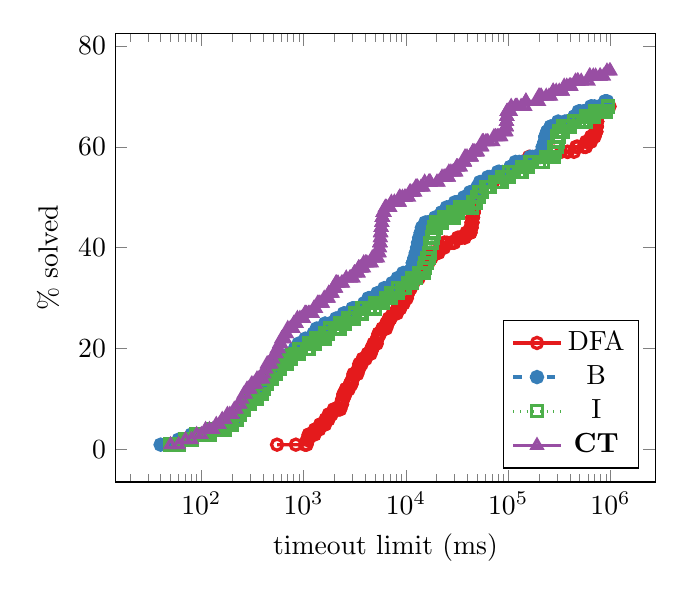
\begin{tikzpicture}[every mark/.append style={mark size=4pt}]%[scale=0.9]
    \begin{axis}[
    xmode=log,
    every axis plot/.style={thin},
    xlabel={timeout limit (ms)},
    ylabel={\% solved},
    legend pos=south east,
    cycle list/Set1-6,
            % define fill color for the marker
            mark list fill={.!75!white},
            mark options={solid},
            cycle multiindex* list={
                Set1-6
                    \nextlist
                [3 of]linestyles
                    \nextlist
                very thick
                \nextlist
                mark=o,
                mark=*,
                mark=square,
                mark=triangle,
                mark=+
            },
    ]

    \addplot
    coordinates {
      (550, 1)
      (840, 1)
      (1030, 1)
      (1070, 1)
      (1080, 2)
      (1090, 2)
      (1100, 2)
      (1110, 2)
      (1120, 3)
      (1130, 3)
      (1140, 3)
      (1170, 3)
      (1180, 3)
      (1190, 3)
      (1280, 3)
      (1290, 4)
      (1300, 4)
      (1340, 4)
      (1360, 4)
      (1420, 4)
      (1450, 5)
      (1460, 5)
      (1550, 5)
      (1590, 5)
      (1610, 5)
      (1620, 5)
      (1640, 6)
      (1650, 6)
      (1680, 6)
      (1740, 6)
      (1750, 6)
      (1760, 7)
      (1780, 7)
      (1810, 7)
      (1830, 7)
      (1880, 7)
      (1970, 8)
      (2010, 8)
      (2070, 8)
      (2160, 8)
      (2180, 8)
      (2240, 8)
      (2280, 8)
      (2300, 9)
      (2320, 9)
      (2340, 9)
      (2360, 9)
      (2370, 9)
      (2380, 10)
      (2400, 10)
      (2420, 10)
      (2430, 10)
      (2440, 10)
      (2450, 11)
      (2460, 11)
      (2480, 11)
      (2490, 11)
      (2550, 11)
      (2560, 11)
      (2590, 12)
      (2600, 12)
      (2620, 12)
      (2630, 12)
      (2750, 12)
      (2760, 12)
      (2830, 13)
      (2840, 13)
      (2880, 13)
      (2910, 13)
      (2930, 13)
      (2940, 13)
      (2990, 14)
      (3000, 14)
      (3010, 14)
      (3030, 14)
      (3070, 15)
      (3160, 15)
      (3190, 15)
      (3250, 15)
      (3260, 15)
      (3290, 15)
      (3350, 15)
      (3400, 16)
      (3430, 16)
      (3450, 16)
      (3480, 16)
      (3500, 17)
      (3550, 17)
      (3630, 17)
      (3650, 17)
      (3700, 17)
      (3780, 18)
      (3830, 18)
      (3870, 18)
      (3950, 18)
      (3960, 18)
      (4050, 18)
      (4220, 19)
      (4320, 19)
      (4340, 19)
      (4350, 19)
      (4520, 19)
      (4590, 20)
      (4600, 20)
      (4640, 20)
      (4670, 20)
      (4680, 20)
      (4710, 20)
      (4820, 21)
      (4870, 21)
      (4940, 21)
      (4950, 21)
      (4980, 21)
      (5180, 21)
      (5210, 22)
      (5220, 22)
      (5240, 22)
      (5260, 22)
      (5270, 22)
      (5280, 22)
      (5400, 23)
      (5430, 23)
      (5480, 23)
      (5520, 23)
      (5590, 23)
      (5880, 24)
      (5930, 24)
      (5970, 24)
      (6170, 24)
      (6280, 24)
      (6400, 24)
      (6420, 25)
      (6460, 25)
      (6530, 25)
      (6620, 25)
      (6630, 25)
      (6650, 25)
      (6800, 26)
      (6960, 26)
      (7020, 26)
      (7040, 26)
      (7090, 26)
      (7430, 27)
      (7750, 27)
      (7760, 27)
      (7790, 27)
      (7880, 27)
      (8170, 27)
      (8240, 28)
      (8300, 28)
      (8310, 28)
      (8610, 28)
      (8770, 28)
      (8800, 28)
      (8950, 29)
      (9050, 29)
      (9240, 29)
      (9270, 29)
      (9380, 29)
      (9410, 29)
      (9500, 29)
      (9580, 30)
      (9650, 30)
      (9840, 30)
      (9950, 30)
      (10200, 30)
      (10380, 31)
      (10400, 31)
      (10410, 31)
      (10450, 31)
      (10460, 31)
      (10490, 31)
      (10540, 32)
      (10760, 32)
      (10890, 32)
      (10970, 32)
      (11060, 32)
      (11170, 32)
      (11200, 33)
      (11440, 33)
      (11550, 33)
      (11610, 33)
      (11620, 33)
      (11820, 33)
      (11860, 34)
      (12230, 34)
      (12550, 34)
      (12670, 34)
      (12770, 34)
      (13100, 34)
      (13360, 34)
      (13500, 35)
      (13640, 35)
      (13740, 35)
      (13820, 35)
      (14310, 35)
      (14320, 35)
      (14490, 36)
      (14650, 36)
      (14920, 36)
      (14940, 36)
      (15080, 36)
      (15140, 36)
      (15490, 36)
      (15660, 37)
      (15680, 37)
      (16050, 37)
      (16070, 37)
      (16230, 37)
      (16600, 37)
      (16730, 38)
      (17030, 38)
      (17090, 38)
      (17400, 38)
      (17510, 38)
      (17800, 38)
      (17990, 39)
      (18580, 39)
      (18870, 39)
      (19950, 39)
      (19980, 39)
      (20460, 39)
      (20820, 39)
      (21550, 40)
      (21800, 40)
      (21960, 40)
      (22580, 40)
      (22650, 40)
      (23570, 40)
      (23810, 41)
      (23840, 41)
      (25170, 41)
      (27570, 41)
      (28160, 41)
      (29400, 41)
      (29590, 41)
      (32170, 42)
      (33320, 42)
      (34310, 42)
      (34450, 42)
      (35060, 42)
      (37590, 42)
      (39070, 43)
      (41030, 43)
      (42030, 43)
      (42110, 43)
      (42560, 43)
      (42590, 43)
      (42690, 43)
      (42720, 44)
      (43170, 44)
      (43570, 44)
      (43610, 44)
      (43620, 44)
      (43860, 44)
      (43880, 45)
      (43970, 45)
      (44060, 45)
      (44510, 45)
      (44590, 45)
      (44620, 45)
      (44670, 46)
      (44690, 46)
      (44850, 46)
      (45080, 46)
      (45130, 46)
      (45140, 46)
      (45650, 47)
      (45720, 47)
      (45810, 47)
      (45840, 47)
      (45870, 47)
      (45910, 47)
      (46000, 48)
      (46230, 48)
      (46310, 48)
      (46580, 48)
      (46600, 48)
      (46640, 48)
      (46680, 48)
      (46730, 49)
      (46880, 49)
      (47010, 49)
      (47040, 49)
      (47130, 49)
      (47520, 49)
      (47760, 50)
      (47990, 50)
      (48040, 50)
      (48180, 50)
      (48400, 50)
      (48420, 50)
      (48490, 50)
      (48500, 51)
      (48510, 51)
      (48630, 51)
      (48710, 51)
      (48880, 51)
      (49120, 51)
      (51040, 52)
      (52050, 52)
      (53070, 52)
      (53920, 52)
      (54160, 52)
      (55650, 52)
      (57610, 53)
      (62030, 53)
      (67210, 53)
      (68040, 53)
      (69500, 53)
      (70070, 53)
      (71260, 53)
      (75510, 54)
      (79160, 54)
      (79890, 54)
      (86410, 54)
      (90560, 54)
      (93850, 54)
      (93910, 55)
      (94840, 55)
      (98270, 55)
      (98610, 55)
      (99880, 55)
      (101600, 55)
      (106800, 55)
      (107940, 56)
      (113230, 56)
      (118040, 56)
      (123230, 56)
      (125250, 56)
      (126460, 56)
      (136850, 57)
      (141410, 57)
      (145590, 57)
      (146260, 57)
      (147100, 57)
      (156470, 57)
      (159560, 58)
      (163380, 58)
      (183150, 58)
      (188630, 58)
      (203020, 58)
      (221140, 58)
      (252130, 58)
      (280600, 59)
      (281920, 59)
      (329390, 59)
      (378010, 59)
      (382430, 59)
      (439630, 59)
      (461470, 60)
      (471890, 60)
      (480190, 60)
      (547470, 60)
      (565750, 60)
      (567980, 60)
      (576020, 60)
      (577420, 61)
      (603180, 61)
      (615930, 61)
      (625640, 61)
      (640580, 61)
      (642660, 61)
      (645690, 62)
      (649280, 62)
      (652550, 62)
      (667400, 62)
      (678420, 62)
      (690100, 62)
      (698600, 62)
      (708040, 63)
      (720000, 63)
      (720800, 63)
      (722220, 63)
      (724200, 63)
      (724530, 63)
      (728770, 64)
      (730570, 64)
      (730590, 64)
      (731370, 64)
      (732210, 64)
      (733600, 64)
      (733910, 65)
      (734530, 65)
      (735560, 65)
      (735840, 65)
      (737480, 65)
      (737920, 65)
      (738690, 65)
      (739660, 66)
      (739730, 66)
      (740600, 66)
      (743400, 66)
      (744510, 66)
      (745370, 66)
      (745640, 67)
      (751150, 67)
      (751910, 67)
      (752040, 67)
      (790090, 67)
      (828510, 67)
      (869340, 67)
      (921350, 68)
      (925960, 68)
      (939670, 68)
      (978230, 68)
      
    };
    \addplot
    coordinates {
      (40, 1)
      (50, 1)
      (60, 2)
      (70, 2)
      (80, 3)
      (90, 3)
      (100, 3)
      (120, 4)
      (130, 4)
      (140, 4)
      (160, 5)
      (170, 5)
      (180, 5)
      (190, 6)
      (200, 6)
      (210, 6)
      (220, 7)
      (230, 7)
      (240, 7)
      (250, 8)
      (260, 8)
      (270, 9)
      (290, 9)
      (300, 10)
      (310, 10)
      (320, 10)
      (330, 10)
      (340, 11)
      (350, 11)
      (360, 11)
      (370, 12)
      (380, 12)
      (390, 12)
      (400, 12)
      (410, 13)
      (420, 13)
      (430, 14)
      (440, 14)
      (450, 14)
      (470, 14)
      (500, 15)
      (510, 15)
      (520, 15)
      (530, 15)
      (540, 16)
      (550, 16)
      (560, 16)
      (570, 17)
      (580, 17)
      (590, 17)
      (610, 17)
      (620, 17)
      (630, 17)
      (640, 18)
      (650, 18)
      (670, 18)
      (690, 18)
      (720, 18)
      (730, 19)
      (780, 19)
      (790, 19)
      (810, 19)
      (820, 20)
      (830, 20)
      (840, 20)
      (850, 20)
      (860, 20)
      (890, 21)
      (920, 21)
      (930, 21)
      (1000, 21)
      (1030, 21)
      (1040, 22)
      (1140, 22)
      (1150, 22)
      (1210, 22)
      (1230, 22)
      (1240, 22)
      (1250, 23)
      (1260, 23)
      (1310, 23)
      (1330, 23)
      (1340, 24)
      (1420, 24)
      (1550, 24)
      (1560, 24)
      (1570, 24)
      (1600, 24)
      (1610, 24)
      (1620, 25)
      (1800, 25)
      (1890, 25)
      (1970, 25)
      (1980, 25)
      (2010, 25)
      (2080, 26)
      (2210, 26)
      (2220, 26)
      (2230, 26)
      (2410, 26)
      (2440, 26)
      (2470, 27)
      (2510, 27)
      (2670, 27)
      (2760, 27)
      (2790, 27)
      (2810, 27)
      (2950, 27)
      (3000, 28)
      (3070, 28)
      (3110, 28)
      (3720, 28)
      (3850, 28)
      (3900, 28)
      (3910, 29)
      (3940, 29)
      (3960, 29)
      (4020, 29)
      (4070, 29)
      (4080, 29)
      (4200, 29)
      (4300, 30)
      (4380, 30)
      (4430, 30)
      (4970, 30)
      (4990, 30)
      (5250, 31)
      (5330, 31)
      (5380, 31)
      (5390, 31)
      (5490, 31)
      (5690, 31)
      (6140, 32)
      (6640, 32)
      (6980, 32)
      (7080, 32)
      (7300, 32)
      (7350, 33)
      (7450, 33)
      (7810, 33)
      (7820, 33)
      (8070, 33)
      (8160, 33)
      (8290, 34)
      (8620, 34)
      (8650, 34)
      (8710, 34)
      (8890, 34)
      (9100, 34)
      (9200, 34)
      (9390, 35)
      (9880, 35)
      (9950, 35)
      (11150, 35)
      (11330, 35)
      (11440, 35)
      (11450, 36)
      (11490, 36)
      (11520, 36)
      (11560, 36)
      (11570, 36)
      (11610, 36)
      (11710, 36)
      (11720, 37)
      (11730, 37)
      (11740, 37)
      (11800, 37)
      (11840, 37)
      (12090, 37)
      (12110, 38)
      (12200, 38)
      (12390, 38)
      (12460, 38)
      (12490, 38)
      (12510, 39)
      (12550, 39)
      (12660, 39)
      (12750, 39)
      (12770, 39)
      (12850, 39)
      (12890, 40)
      (12910, 40)
      (13000, 40)
      (13010, 40)
      (13020, 40)
      (13180, 41)
      (13190, 41)
      (13330, 41)
      (13380, 41)
      (13400, 41)
      (13490, 42)
      (13650, 42)
      (13710, 42)
      (13720, 42)
      (13880, 42)
      (14000, 43)
      (14020, 43)
      (14060, 43)
      (14070, 43)
      (14180, 43)
      (14190, 43)
      (14250, 43)
      (14330, 44)
      (14640, 44)
      (14810, 44)
      (15030, 44)
      (15280, 44)
      (15330, 44)
      (15450, 45)
      (16080, 45)
      (16490, 45)
      (16840, 45)
      (17230, 45)
      (17370, 45)
      (19310, 46)
      (19860, 46)
      (20520, 46)
      (20670, 46)
      (20950, 46)
      (21010, 46)
      (21410, 46)
      (22390, 47)
      (22400, 47)
      (23060, 47)
      (23670, 47)
      (23770, 47)
      (23990, 47)
      (25040, 48)
      (26030, 48)
      (27860, 48)
      (28430, 48)
      (29420, 48)
      (29430, 48)
      (29770, 48)
      (30130, 49)
      (31300, 49)
      (31470, 49)
      (32360, 49)
      (36130, 49)
      (36670, 49)
      (36960, 50)
      (37610, 50)
      (39020, 50)
      (39870, 50)
      (40280, 50)
      (41080, 50)
      (42090, 50)
      (42340, 51)
      (42730, 51)
      (44460, 51)
      (46790, 51)
      (47300, 51)
      (48720, 51)
      (49900, 52)
      (50190, 52)
      (50380, 52)
      (51560, 52)
      (51670, 52)
      (52930, 52)
      (53070, 53)
      (53180, 53)
      (55820, 53)
      (57090, 53)
      (57910, 53)
      (61660, 53)
      (62930, 53)
      (63380, 54)
      (65710, 54)
      (70600, 54)
      (70870, 54)
      (72970, 54)
      (77350, 54)
      (79280, 55)
      (79890, 55)
      (81410, 55)
      (81770, 55)
      (81780, 55)
      (87640, 55)
      (101330, 55)
      (105170, 56)
      (105410, 56)
      (105640, 56)
      (109260, 56)
      (115720, 56)
      (117110, 56)
      (117810, 57)
      (128530, 57)
      (140070, 57)
      (144570, 57)
      (145440, 57)
      (146750, 57)
      (164060, 58)
      (173000, 58)
      (183390, 58)
      (189860, 58)
      (203540, 58)
      (204830, 58)
      (207670, 58)
      (212230, 59)
      (214190, 59)
      (214370, 59)
      (215170, 59)
      (215850, 59)
      (216790, 59)
      (217510, 60)
      (218870, 60)
      (219890, 60)
      (223170, 60)
      (224760, 60)
      (225170, 60)
      (225860, 60)
      (226850, 61)
      (227440, 61)
      (228660, 61)
      (229240, 61)
      (230000, 61)
      (231220, 62)
      (231360, 62)
      (231560, 62)
      (231610, 62)
      (232280, 62)
      (235010, 62)
      (235380, 62)
      (240580, 63)
      (241080, 63)
      (241120, 63)
      (247070, 63)
      (253910, 63)
      (259150, 63)
      (259930, 64)
      (260450, 64)
      (269680, 64)
      (290930, 64)
      (293180, 64)
      (301170, 64)
      (307460, 65)
      (358130, 65)
      (373680, 65)
      (395010, 65)
      (400330, 65)
      (415600, 65)
      (417390, 65)
      (444260, 66)
      (445130, 66)
      (449310, 66)
      (474370, 66)
      (482150, 66)
      (482210, 66)
      (487090, 67)
      (500040, 67)
      (502640, 67)
      (542500, 67)
      (550590, 67)
      (553150, 67)
      (566020, 67)
      (645270, 68)
      (653190, 68)
      (697470, 68)
      (777770, 68)
      (794860, 68)
      (879060, 68)
      (886150, 69)
      (896370, 69)
      (901390, 69)
      (901730, 69)
      (925510, 69)
      
    };
    \addplot
    coordinates {
      (50, 1)
      (60, 1)
      (70, 2)
      (80, 2)
      (90, 3)
      (100, 3)
      (110, 3)
      (120, 3)
      (130, 4)
      (140, 4)
      (150, 4)
      (160, 4)
      (170, 4)
      (180, 5)
      (190, 5)
      (200, 5)
      (220, 6)
      (230, 7)
      (240, 7)
      (250, 8)
      (260, 8)
      (270, 9)
      (280, 9)
      (290, 9)
      (300, 9)
      (310, 10)
      (320, 10)
      (340, 10)
      (350, 10)
      (360, 11)
      (380, 11)
      (390, 11)
      (400, 12)
      (410, 12)
      (420, 13)
      (430, 13)
      (440, 13)
      (450, 14)
      (460, 14)
      (470, 14)
      (490, 14)
      (500, 15)
      (520, 15)
      (530, 15)
      (540, 16)
      (550, 16)
      (560, 16)
      (570, 16)
      (580, 16)
      (600, 17)
      (630, 17)
      (650, 17)
      (660, 17)
      (690, 17)
      (720, 18)
      (730, 18)
      (750, 18)
      (770, 19)
      (820, 19)
      (860, 19)
      (870, 19)
      (890, 19)
      (900, 20)
      (910, 20)
      (930, 20)
      (940, 20)
      (1090, 20)
      (1120, 20)
      (1130, 21)
      (1150, 21)
      (1170, 21)
      (1180, 21)
      (1280, 21)
      (1290, 21)
      (1330, 22)
      (1400, 22)
      (1500, 22)
      (1550, 22)
      (1560, 22)
      (1610, 22)
      (1620, 23)
      (1630, 23)
      (1700, 23)
      (1720, 23)
      (1730, 23)
      (1810, 24)
      (2050, 24)
      (2150, 24)
      (2180, 24)
      (2190, 24)
      (2220, 24)
      (2250, 24)
      (2270, 25)
      (2290, 25)
      (2320, 25)
      (2470, 25)
      (2540, 25)
      (2700, 26)
      (2740, 26)
      (2880, 26)
      (2910, 26)
      (3080, 26)
      (3120, 26)
      (3200, 27)
      (3550, 27)
      (3580, 27)
      (3660, 27)
      (3680, 27)
      (3700, 27)
      (3770, 28)
      (3870, 28)
      (4370, 28)
      (4390, 28)
      (4460, 28)
      (5010, 28)
      (5060, 29)
      (5190, 29)
      (5330, 29)
      (5410, 29)
      (5510, 29)
      (5710, 29)
      (5980, 29)
      (6470, 30)
      (6700, 30)
      (6780, 30)
      (6810, 30)
      (6980, 30)
      (7070, 30)
      (7220, 31)
      (7650, 31)
      (7850, 31)
      (7950, 31)
      (7980, 31)
      (8140, 31)
      (8240, 31)
      (8400, 32)
      (9230, 32)
      (9260, 32)
      (9320, 32)
      (9390, 32)
      (9810, 32)
      (10590, 33)
      (11030, 33)
      (11090, 33)
      (11240, 33)
      (11370, 33)
      (11400, 33)
      (11570, 34)
      (11630, 34)
      (11880, 34)
      (12210, 34)
      (12510, 34)
      (12520, 34)
      (12550, 34)
      (13520, 35)
      (14450, 35)
      (14750, 35)
      (14800, 35)
      (15040, 35)
      (15080, 36)
      (15130, 36)
      (15210, 36)
      (15370, 36)
      (15390, 36)
      (15410, 37)
      (15470, 37)
      (15620, 37)
      (15980, 37)
      (16100, 37)
      (16150, 37)
      (16190, 38)
      (16490, 38)
      (16590, 38)
      (16640, 38)
      (16680, 38)
      (16720, 38)
      (16750, 39)
      (16800, 39)
      (16870, 39)
      (16950, 39)
      (17070, 39)
      (17090, 39)
      (17100, 40)
      (17130, 40)
      (17170, 40)
      (17180, 40)
      (17190, 40)
      (17220, 40)
      (17300, 41)
      (17550, 41)
      (17730, 41)
      (17760, 41)
      (17820, 41)
      (17950, 41)
      (17980, 41)
      (18060, 42)
      (18080, 42)
      (18100, 42)
      (18150, 42)
      (18230, 42)
      (18330, 42)
      (18460, 43)
      (18480, 43)
      (18580, 43)
      (18590, 43)
      (18700, 43)
      (18840, 43)
      (18920, 43)
      (18960, 44)
      (19300, 44)
      (19410, 44)
      (19560, 44)
      (19570, 44)
      (19640, 44)
      (19760, 45)
      (19830, 45)
      (20370, 45)
      (21220, 45)
      (21880, 45)
      (22610, 45)
      (23680, 46)
      (24090, 46)
      (25400, 46)
      (25580, 46)
      (26310, 46)
      (27720, 46)
      (29250, 46)
      (29300, 47)
      (29420, 47)
      (30980, 47)
      (31300, 47)
      (31430, 47)
      (32120, 47)
      (33870, 48)
      (34700, 48)
      (36390, 48)
      (37860, 48)
      (38390, 48)
      (40430, 48)
      (44370, 48)
      (45220, 49)
      (45850, 49)
      (46730, 49)
      (47040, 49)
      (47590, 49)
      (47970, 49)
      (49360, 50)
      (49800, 50)
      (50400, 50)
      (50510, 50)
      (50780, 50)
      (51450, 50)
      (51540, 51)
      (51650, 51)
      (52320, 51)
      (53220, 51)
      (53570, 51)
      (55250, 51)
      (61360, 52)
      (61840, 52)
      (64020, 52)
      (64590, 52)
      (65270, 52)
      (65960, 52)
      (75460, 53)
      (80010, 53)
      (80590, 53)
      (80850, 53)
      (82360, 53)
      (84470, 53)
      (85710, 53)
      (88220, 54)
      (90130, 54)
      (90670, 54)
      (93840, 54)
      (95870, 54)
      (100350, 54)
      (101240, 55)
      (112490, 55)
      (113550, 55)
      (127990, 55)
      (129810, 55)
      (131940, 55)
      (137030, 55)
      (137140, 56)
      (138470, 56)
      (140790, 56)
      (147540, 56)
      (156920, 56)
      (157130, 56)
      (162560, 57)
      (162760, 57)
      (169630, 57)
      (170370, 57)
      (198730, 57)
      (219630, 57)
      (236800, 58)
      (248230, 58)
      (259520, 58)
      (265820, 58)
      (273280, 58)
      (276470, 58)
      (279690, 58)
      (280230, 59)
      (281590, 59)
      (281810, 59)
      (282220, 59)
      (282390, 59)
      (284210, 59)
      (284410, 60)
      (286450, 60)
      (288270, 60)
      (288290, 60)
      (292840, 60)
      (295540, 60)
      (296190, 60)
      (298980, 61)
      (299550, 61)
      (299870, 61)
      (300160, 61)
      (300600, 61)
      (302190, 61)
      (303070, 62)
      (303280, 62)
      (307930, 62)
      (308440, 62)
      (311430, 62)
      (312510, 62)
      (313510, 62)
      (315280, 63)
      (317550, 63)
      (322930, 63)
      (329550, 63)
      (342630, 63)
      (343570, 63)
      (346140, 64)
      (353150, 64)
      (361750, 64)
      (374030, 64)
      (382470, 64)
      (404230, 64)
      (437270, 65)
      (492850, 65)
      (494920, 65)
      (538040, 65)
      (551680, 65)
      (565550, 65)
      (577170, 65)
      (581290, 66)
      (583270, 66)
      (606290, 66)
      (649170, 66)
      (680520, 66)
      (689910, 66)
      (716250, 67)
      (770340, 67)
      (809510, 67)
      (812480, 67)
      (861730, 67)
      (862310, 67)
      (908880, 67)
      (945850, 68)
      (946540, 68)
      
    };
    \addplot
    coordinates {
      (50, 1)
      (60, 1)
      (70, 2)
      (80, 2)
      (90, 3)
      (100, 3)
      (110, 4)
      (120, 4)
      (130, 4)
      (140, 5)
      (150, 5)
      (160, 6)
      (170, 6)
      (180, 7)
      (190, 7)
      (200, 7)
      (210, 8)
      (220, 8)
      (230, 9)
      (240, 9)
      (250, 10)
      (260, 11)
      (270, 11)
      (280, 12)
      (290, 12)
      (300, 12)
      (310, 13)
      (320, 13)
      (340, 13)
      (350, 14)
      (360, 14)
      (390, 14)
      (400, 14)
      (410, 15)
      (420, 16)
      (430, 16)
      (440, 17)
      (450, 17)
      (460, 17)
      (470, 17)
      (480, 17)
      (490, 18)
      (500, 18)
      (520, 19)
      (530, 19)
      (540, 19)
      (550, 20)
      (560, 20)
      (570, 20)
      (580, 21)
      (590, 21)
      (600, 21)
      (610, 22)
      (620, 22)
      (640, 22)
      (650, 22)
      (670, 23)
      (680, 23)
      (700, 24)
      (740, 24)
      (750, 24)
      (760, 24)
      (790, 24)
      (800, 25)
      (820, 25)
      (840, 25)
      (850, 25)
      (870, 26)
      (920, 26)
      (950, 26)
      (970, 26)
      (1000, 26)
      (1030, 27)
      (1040, 27)
      (1070, 27)
      (1120, 27)
      (1150, 27)
      (1180, 27)
      (1220, 27)
      (1260, 28)
      (1270, 28)
      (1290, 28)
      (1310, 28)
      (1370, 29)
      (1410, 29)
      (1420, 29)
      (1450, 29)
      (1500, 29)
      (1520, 29)
      (1530, 29)
      (1590, 30)
      (1700, 30)
      (1710, 30)
      (1750, 30)
      (1760, 31)
      (1830, 31)
      (1840, 31)
      (1880, 31)
      (1910, 31)
      (1940, 32)
      (1950, 32)
      (1970, 32)
      (2040, 32)
      (2060, 32)
      (2070, 33)
      (2080, 33)
      (2110, 33)
      (2170, 33)
      (2350, 33)
      (2410, 33)
      (2610, 34)
      (2830, 34)
      (2860, 34)
      (2900, 34)
      (3040, 34)
      (3050, 34)
      (3130, 35)
      (3140, 35)
      (3340, 35)
      (3410, 35)
      (3420, 35)
      (3450, 36)
      (3460, 36)
      (3560, 36)
      (3610, 36)
      (3660, 36)
      (3710, 36)
      (3860, 36)
      (3870, 37)
      (4040, 37)
      (4150, 37)
      (4410, 37)
      (4610, 37)
      (4690, 38)
      (4910, 38)
      (4970, 38)
      (5020, 38)
      (5070, 38)
      (5290, 38)
      (5340, 39)
      (5350, 39)
      (5380, 39)
      (5470, 39)
      (5480, 39)
      (5490, 40)
      (5510, 40)
      (5530, 40)
      (5540, 41)
      (5550, 41)
      (5560, 41)
      (5570, 41)
      (5590, 41)
      (5610, 41)
      (5620, 42)
      (5630, 42)
      (5640, 43)
      (5650, 43)
      (5670, 43)
      (5680, 43)
      (5700, 44)
      (5710, 44)
      (5730, 44)
      (5740, 44)
      (5760, 44)
      (5780, 45)
      (5790, 45)
      (5820, 45)
      (5830, 45)
      (5840, 46)
      (5850, 46)
      (5870, 46)
      (5900, 46)
      (5910, 46)
      (5920, 46)
      (5940, 46)
      (5960, 47)
      (5970, 47)
      (5980, 47)
      (6030, 47)
      (6090, 47)
      (6150, 47)
      (6280, 48)
      (6340, 48)
      (6480, 48)
      (6840, 48)
      (6970, 48)
      (7210, 49)
      (7710, 49)
      (7730, 49)
      (8490, 49)
      (8620, 49)
      (8630, 49)
      (8660, 50)
      (8750, 50)
      (9250, 50)
      (9750, 50)
      (9790, 50)
      (9980, 50)
      (10650, 50)
      (10890, 51)
      (11070, 51)
      (11130, 51)
      (11520, 51)
      (11740, 51)
      (12240, 51)
      (12470, 52)
      (12750, 52)
      (12870, 52)
      (13000, 52)
      (14050, 52)
      (14780, 52)
      (15250, 53)
      (16740, 53)
      (17090, 53)
      (17150, 53)
      (17300, 53)
      (20090, 53)
      (20650, 53)
      (22530, 54)
      (23590, 54)
      (24080, 54)
      (24600, 54)
      (25950, 54)
      (26010, 54)
      (26310, 55)
      (27520, 55)
      (28910, 55)
      (29020, 55)
      (29830, 55)
      (30330, 55)
      (30860, 55)
      (31320, 56)
      (31440, 56)
      (31810, 56)
      (32180, 56)
      (33910, 56)
      (34120, 56)
      (36930, 57)
      (36940, 57)
      (37060, 57)
      (37240, 57)
      (37300, 57)
      (37490, 57)
      (37850, 58)
      (39550, 58)
      (42240, 58)
      (42540, 58)
      (43230, 58)
      (43500, 58)
      (43650, 58)
      (44950, 59)
      (45410, 59)
      (46610, 59)
      (48590, 59)
      (49050, 59)
      (50170, 59)
      (53630, 60)
      (54160, 60)
      (54430, 60)
      (54450, 60)
      (54490, 60)
      (54920, 60)
      (55330, 60)
      (55870, 61)
      (57260, 61)
      (60490, 61)
      (62160, 61)
      (63280, 61)
      (71010, 61)
      (72590, 62)
      (75040, 62)
      (75370, 62)
      (78200, 62)
      (80830, 62)
      (83350, 62)
      (84800, 62)
      (90460, 63)
      (92080, 63)
      (93140, 63)
      (93590, 63)
      (94730, 63)
      (94900, 63)
      (94980, 64)
      (95250, 64)
      (95500, 64)
      (95540, 64)
      (95730, 64)
      (95770, 64)
      (95780, 65)
      (95870, 65)
      (96110, 65)
      (96160, 65)
      (96170, 65)
      (96290, 65)
      (96430, 65)
      (96470, 66)
      (96520, 66)
      (96920, 66)
      (96930, 66)
      (97190, 66)
      (97330, 66)
      (97410, 67)
      (97580, 67)
      (97630, 67)
      (100660, 67)
      (102990, 67)
      (103230, 67)
      (105320, 67)
      (106900, 68)
      (117510, 68)
      (120220, 68)
      (122290, 68)
      (133710, 68)
      (145720, 68)
      (148400, 69)
      (149210, 69)
      (149390, 69)
      (188660, 69)
      (190110, 69)
      (198370, 69)
      (199080, 70)
      (203260, 70)
      (205030, 70)
      (210860, 70)
      (235310, 70)
      (250470, 70)
      (260550, 70)
      (274190, 71)
      (275860, 71)
      (294700, 71)
      (315240, 71)
      (338260, 71)
      (339770, 71)
      (352710, 72)
      (373740, 72)
      (395750, 72)
      (399990, 72)
      (407380, 72)
      (409390, 72)
      (410490, 72)
      (454610, 73)
      (474090, 73)
      (476710, 73)
      (482760, 73)
      (517330, 73)
      (606460, 73)
      (623230, 74)
      (630420, 74)
      (679300, 74)
      (716240, 74)
      (788320, 74)
      (796770, 74)
      (855630, 74)
      (923830, 75)
      (980220, 75)
      (995840, 75)
      
    };
    

    \legend{ DFA, B, I, \textbf{CT} }
  \end{axis}

  \end{tikzpicture}
  \caption{Percentage of instances solved as a funcion of time for the DFA, B, I, and CT 
    propagators.}
  \label{fig:total}
\end{figure}

The plots from each individual group of benchmarks are presented 
in Appendix~\ref{app:compare-gecode},
except for the groups \emph{BDD Small}, where DFA ran out of memory on all instances,
and \emph{MDD 07} and \emph{MDD 09}, 
where all propagators timed out on all instances.

\subsubsection{Discussion}

\paragraph{Runtime.}
CT performs either as well as or better than all other propagators,
on all groups except \emph{AIM 200}, where CT was slightly slower than B and DFA
on two instances, and on \emph{BDD Large} where CT was slightly
slower than B and I on the small instances. At best, CT is about a factor 10 faster
than the other algorithms on some groups.
CT could solve as many instances as, or more, than all other propagators,
on all groups except \emph{Pigeons Plus} where DFA could solve one more instance.

Another notable observation is that B seems to outperform I, even though I is said to
be more efficient than B in terms of execution speed.

On the various groups the performance gain from CT varies, which might depend
on the characteristics for the different groups of benchmarks. Here the impact
of \emph{table size}, \emph{arity} and \emph{domain size} on runtime performance
is discussed:

\begin{description}
  \item[Table size] The increase
    of performance for CT compared to the other propagators
    is larger on the groups that contain 
    instances with large table sizes only (see \emph{A5}, \emph{A10},
    \emph{K5}, \emph{MDD 05}, and \emph{Rands JC*}), than on the groups
    that contain only small tables (see \emph{AIM-*}, \emph{Dubois}, and \emph{Geom}).
    
    The property shows particularly well on the four \emph{Rands JC*} groups, where
    arity and domain size are constant while the table size increases from
    $2500$ to~$10000$ in steps of~$2500$. On these groups, the performance gain
    seems to increase with an increasing table size.

    \item[Arity] Many groups where CT shows little or none performance gain have
      constraints with low arities (see \emph{AIM-*}, \emph{Dubois}, \emph{Geom},
      \emph{Langford *}), though there are exceptions to this (see \emph{Pigeons Plus},
      \emph{TSP *}). 
      However, the groups with low arities also have small tables, while the groups
      with larger arities tend to have larger tables, which makes it hard to
      tell whether it is the arity or the table size that impact the performance gain.
      
    \item[Domain size] It is hard to draw any conclusions of whether the domain size affects
      the performance gain of CT. Among the groups with small domain sizes, some
      have little or no performance gains (see \emph{AIM-*}, \emph{Dubois}) and
      some have large performance gains (see \emph{MDD 05}, \emph{BDD Large}).
      The same is true for the groups with larger domain sizes; some have
      modest performance gains (see \emph{Nonograms}, \emph{Kakuro *}),
      while some have larger performance gains (see \emph{Rands JC*}, \emph{Crosswords *}).
\end{description}

\paragraph{Memory usage.}
It can be seen that CT, B, and I has about the same maximum memory usage 
while DFA consistently has a higher maximum memory usage.
  
\paragraph{Profiling.}
It can be seen that the distribution of how the time is spent between propagation, advisors
and copying varies between different propagators and different groups of benchmarks.
% Benchmarks: performance beroende på antalet variabler. 2-ställiga, 3-ställiga, ..., n-ställiga
\section{Conclusions and Future Work}
\label{conclusions}

In this bachelor thesis project, a new propagator algorithm for the~\Table~constraint,
called Compact-Table (CT), was implemented in the constraint solver Gecode, and its performance
was evaluated compared to the existing propagators for~\Table~in Gecode, as well
as the propagator for the \Constraint{Regular} constraint.
The result of the evaluation is that CT outperforms the existing propagators
in Gecode for \Table, which suggests that CT should be included in the solver.
The performance gains from CT seem to be largest for constraints with large tables,
and more modest for constraints with small tables.

For the implementation to reach production quality, there
are a few things that need to be revised. The following lists some known
improvements and flaws:

\begin{itemize}
    
  \item Some memory allocations in the initialisation of the propagator
    depend on the domain widths rather
    than the domain sizes of the variables. This is unsustainable
    for pathological domains such as $\Set{1, 10^9}$. In the current
    implementation, a memory block of size~$10^9$ is allocated for this
    domain, but ideally it should not be necessary to allocate more than~$2$
    elements.

  \item The threshold value for when to use a hash table versus
    an array for indexing the supports should be calibrated with
    experiments.

  \item In the variant using delta information, the current implementation
    uses the incremental update if~$|\Delta_x| < |s(x)|$. It is possible
    that this condition can be generalised to~$|\Delta_x| < k \cdot |s(x)|$,
    for some suitable~$k \in \mathbb{R}$; this is something that remains 
    to be investigated.
    
  \item For \Table~constraints involving a small number (at most $64$)
    tuples, the implementation could be simplified, which would save
    memory and possibly increase execution speed.

  \item Implement the generalisations of the CT algorithm described
    in~\cite{DBLP:conf/aaai/VerhaegheLS17}.

\end{itemize}

\bibliographystyle{abbrv}
\bibliography{astra,mybib}


% \appendix
% \section{Source Code}
% \label{sec:source-code}


% % This appendix presents the source code for the implementation
% % described in \Chapref{sec:implementation}.
% \newpage
\newpage
\appendix
\section{Plots from Comparison of Different Versions of CT}
\label{app:compare-ct}
% the \\ insures the section title is centered below the phrase: AppendixA

Each plot shows the percentage of instances solved as a function
of timeout limit in milliseconds. The measured time is the total
runtime, including parsing the model and the posting
the propagators.

\vspace{2cm}

\begin{figure}[H]
  \begin{minipage}[b][8cm][s]{0.45\textwidth}
    \centering
    \vfill
    \begin{tikzpicture}[scale=0.9]
      \begin{axis}[
    xmode=log,
    ymin=0,ymax=10,
    xmin=0.1, xmax=1000000,
    every axis plot/.style={thin},
    xlabel={timeout limit (ms)},
    ylabel={\# solved},
    legend pos=south east
    % table/create on use/cumulative distribution/.style={
    %   create col/expr={\pgfmathaccuma + \thisrow{f(x)}}   
    % }
    ]
    \addplot 
    [mark=triangle*,
    mark size=1.5,
    mark options={solid},
    green] 
    coordinates {
    (493.707, 1)
(1534.065, 2)
(1732.300, 3)
(1892.718, 4)
(4819.172, 5)
(5753.130, 6)
(9028.954, 7)
(12217.926, 8)
(14965.073, 9)
(63087.240, 10)
    };

    \addplot 
    [blue,
    mark=*,
    mark size=1.5,
    mark options={solid}]
    coordinates {
    (390.154, 1)
(1197.210, 2)
(1390.971, 3)
(1519.242, 4)
(3823.828, 5)
(4617.781, 6)
(7228.985, 7)
(9919.531, 8)
(11845.924, 9)
(49761.700, 10)
    };

    \addplot [brown!60!black,
    mark options={fill=brown!40},
    mark=otimes*,
    mark size=1.5]
    coordinates {
    (497.095, 1)
(1524.837, 2)
(1760.207, 3)
(1913.266, 4)
(4875.522, 5)
(5784.823, 6)
(9099.779, 7)
(12223.350, 8)
(15056.924, 9)
(63609.035, 10)
    };

    \addplot 
    [red,
    mark size=1.5,
    mark=square*]
    coordinates {
    (594.196, 1)
(1881.198, 2)
(2139.673, 3)
(2268.559, 4)
(5854.235, 5)
(7115.928, 6)
(10970.686, 7)
(15071.509, 8)
(18836.865, 9)
(78418.083, 10)
    };
    \legend{CT,CT($\Delta$),CT(randsJC2500$),CT($)}
  \end{axis}

    \end{tikzpicture}
    \vfill
    \caption{\textbf{Rands JC2500.} }
    \vspace{\baselineskip}
  \end{minipage}\qquad
  \begin{minipage}[b][8cm][s]{0.45\textwidth}
    \centering
    \vfill
    \begin{tikzpicture}[scale=0.9]
      \begin{tikzpicture}[scale=1.0]
  \begin{axis}[
    xmode=log,
    ymin=0,ymax=10,
    xmin=0.1, xmax=1000000,
    every axis plot/.style={thin},
    xlabel={timeout limit (ms)},
    ylabel={\# solved},
    legend pos=south east
    % table/create on use/cumulative distribution/.style={
    %   create col/expr={\pgfmathaccuma + \thisrow{f(x)}}   
    % }
    ]
    \addplot 
    [mark=triangle*,
    mark size=1.5,
    mark options={solid},
    green] 
    coordinates {(4628.944, 1)
(5269.761, 2)
(7834.109, 3)
(10221.080, 4)
(42344.662, 5)
(46622.351, 6)
(62439.762, 7)
(116797.805, 8)
(180486.235, 9)
(300000.216, 10)};

    \addplot 
    [blue,
    mark=*,
    mark size=1.5,
    mark options={solid}]
    coordinates {(3528.185, 1)
(4146.147, 2)
(5942.940, 3)
(7947.450, 4)
(33338.965, 5)
(35886.866, 6)
(48586.026, 7)
(93315.398, 8)
(137662.304, 9)
(300000.350, 10)};

    \addplot [brown!60!black,
    mark options={fill=brown!40},
    mark=otimes*,
    mark size=1.5]
    coordinates {(4618.235, 1)
(5129.404, 2)
(7790.409, 3)
(10206.794, 4)
(43367.029, 5)
(46391.923, 6)
(61868.162, 7)
(116295.050, 8)
(181630.843, 9)
(300000.256, 10)};

    \addplot 
    [red,
    mark size=1.5,
    mark=square*]
    coordinates {(5663.567, 1)
(6586.833, 2)
(10111.497, 3)
(12848.274, 4)
(53494.054, 5)
(58301.293, 6)
(77295.794, 7)
(147053.910, 8)
(229203.930, 9)
(300000.278, 10)};
    \legend{CT,D,F,L}
  \end{axis}
\end{tikzpicture}

    \end{tikzpicture}
    \vfill
    \caption{\textbf{Rands JC5000}. }
    \vspace{\baselineskip}
  \end{minipage}\qquad
\end{figure}
\begin{figure}[H]
  \begin{minipage}[b][8cm][s]{0.45\textwidth}
    \centering
    \vfill
    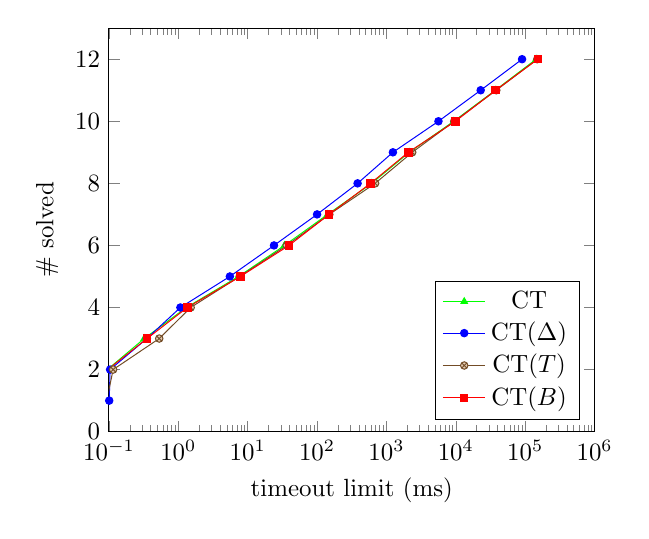
\begin{tikzpicture}[scale=0.9]
        \begin{axis}[
    xmode=log,
    ymin=0,ymax=13,
    xmin=0.1, xmax=1000000,
    every axis plot/.style={thin},
    xlabel={timeout limit (ms)},
    ylabel={\# solved},
    legend pos=south east
    % table/create on use/cumulative distribution/.style={
    %   create col/expr={\pgfmathaccuma + \thisrow{f(x)}}   
    % }
    ]
    \addplot 
    [mark=triangle*,
    mark size=1.5,
    mark options={solid},
    green] 
    coordinates {(0.092, 1)
(0.095, 2)
(0.323, 3)
(1.305, 4)
(7.407, 5)
(33.999, 6)
(142.189, 7)
(612.106, 8)
(2128.536, 9)
(9342.811, 10)
(37031.905, 11)
(143593.524, 12)};

    \addplot 
    [blue,
    mark=*,
    mark size=1.5,
    mark options={solid}]
    coordinates {(0.101, 1)
(0.104, 2)
(0.352, 3)
(1.072, 4)
(5.534, 5)
(23.943, 6)
(100.074, 7)
(383.914, 8)
(1238.844, 9)
(5618.200, 10)
(22809.152, 11)
(90056.907, 12)};

    \addplot [brown!60!black,
    mark options={fill=brown!40},
    mark=otimes*,
    mark size=1.5]
    coordinates {(0.093, 1)
(0.115, 2)
(0.531, 3)
(1.508, 4)
(7.667, 5)
(36.564, 6)
(150.260, 7)
(687.096, 8)
(2352.488, 9)
(9484.143, 10)
(38304.007, 11)
(149005.215, 12)};

    \addplot 
    [red,
    mark size=1.5,
    mark=square*]
    coordinates {(0.095, 1)
(0.096, 2)
(0.355, 3)
(1.348, 4)
(7.869, 5)
(39.453, 6)
(149.173, 7)
(590.206, 8)
(2064.396, 9)
(9858.869, 10)
(37441.670, 11)
(151868.885, 12)};
    \legend{CT,CT($\Delta$),CT($T$),CT($B$)}
  \end{axis}

    \end{tikzpicture}
    \vfill
    \caption{\textbf{Langford 4}.}
    \vspace{\baselineskip}
  \end{minipage}\qquad
  \begin{minipage}[b][8cm][s]{0.45\textwidth}
    \centering
    \vfill
    \begin{tikzpicture}[scale=0.9]
      \begin{tikzpicture}[scale=1.0]
  \begin{axis}[
    xmode=log,
    ymin=0,ymax=50,
    xmin=0.1, xmax=1000000,
    every axis plot/.style={thin},
    xlabel={timeout limit (ms)},
    ylabel={\# solved},
    legend pos=south east
    % table/create on use/cumulative distribution/.style={
    %   create col/expr={\pgfmathaccuma + \thisrow{f(x)}}   
    % }
    ]
    \addplot 
    [mark=triangle*,
    mark size=1.5,
    mark options={solid},
    green] 
    coordinates {(4616.454, 1)
(4618.833, 2)
(4940.533, 3)
(4966.402, 4)
(5022.930, 5)
(5116.613, 6)
(5130.681, 7)
(5134.031, 8)
(5193.654, 9)
(5285.091, 10)
(5305.009, 11)
(5328.617, 12)
(5371.012, 13)
(5388.793, 14)
(5410.720, 15)
(5441.997, 16)
(5455.481, 17)
(5578.855, 18)
(5641.853, 19)
(5648.097, 20)
(5672.192, 21)
(5679.702, 22)
(5683.292, 23)
(5719.242, 24)
(5725.902, 25)
(5734.356, 26)
(5760.307, 27)
(5771.703, 28)
(5797.243, 29)
(5849.862, 30)
(5898.012, 31)
(5937.207, 32)
(6002.529, 33)
(6019.686, 34)
(6119.094, 35)
(6158.836, 36)
(6199.964, 37)
(6257.022, 38)
(6279.015, 39)
(6296.990, 40)
(6352.257, 41)
(6430.852, 42)
(6432.519, 43)
(6470.687, 44)
(6490.446, 45)
(6539.759, 46)
(6552.644, 47)
(6577.534, 48)
(6645.354, 49)
(6760.127, 50)};

    \addplot 
    [blue,
    mark=*,
    mark size=1.5,
    mark options={solid}]
    coordinates {(2221.627, 1)
(2406.818, 2)
(2410.417, 3)
(2478.595, 4)
(2494.484, 5)
(2610.324, 6)
(2662.381, 7)
(2699.699, 8)
(2701.623, 9)
(2705.606, 10)
(2723.756, 11)
(2737.326, 12)
(2765.084, 13)
(2766.971, 14)
(2799.027, 15)
(2809.753, 16)
(2858.020, 17)
(2883.670, 18)
(2887.618, 19)
(2899.053, 20)
(2909.206, 21)
(2912.107, 22)
(2971.321, 23)
(2982.026, 24)
(3005.557, 25)
(3013.018, 26)
(3025.735, 27)
(3030.892, 28)
(3114.959, 29)
(3119.511, 30)
(3123.651, 31)
(3124.390, 32)
(3148.031, 33)
(3176.451, 34)
(3193.730, 35)
(3266.242, 36)
(3304.264, 37)
(3313.805, 38)
(3330.655, 39)
(3362.242, 40)
(3371.608, 41)
(3501.498, 42)
(3523.099, 43)
(3530.659, 44)
(3556.029, 45)
(3582.482, 46)
(3592.317, 47)
(3604.448, 48)
(3685.513, 49)
(3744.809, 50)};

    \addplot [brown!60!black,
    mark options={fill=brown!40},
    mark=otimes*,
    mark size=1.5]
    coordinates {(4666.117, 1)
(4884.063, 2)
(5090.625, 3)
(5188.099, 4)
(5305.729, 5)
(5361.245, 6)
(5455.278, 7)
(5457.351, 8)
(5473.296, 9)
(5522.072, 10)
(5560.972, 11)
(5598.913, 12)
(5605.940, 13)
(5609.929, 14)
(5654.246, 15)
(5661.025, 16)
(5716.926, 17)
(5727.477, 18)
(5742.211, 19)
(5789.404, 20)
(5869.049, 21)
(5875.201, 22)
(5891.779, 23)
(5911.066, 24)
(5919.859, 25)
(5927.269, 26)
(6068.873, 27)
(6113.292, 28)
(6171.700, 29)
(6197.012, 30)
(6241.185, 31)
(6308.864, 32)
(6314.385, 33)
(6328.125, 34)
(6361.133, 35)
(6450.681, 36)
(6454.027, 37)
(6480.689, 38)
(6493.962, 39)
(6503.325, 40)
(6578.864, 41)
(6597.842, 42)
(6626.283, 43)
(6635.984, 44)
(6662.996, 45)
(6684.042, 46)
(6880.051, 47)
(6924.437, 48)
(7090.997, 49)
(7478.901, 50)};

    \addplot 
    [red,
    mark size=1.5,
    mark=square*]
    coordinates {(5703.521, 1)
(5738.525, 2)
(6124.676, 3)
(6219.223, 4)
(6269.173, 5)
(6319.573, 6)
(6395.842, 7)
(6475.436, 8)
(6503.743, 9)
(6517.282, 10)
(6560.928, 11)
(6588.592, 12)
(6615.815, 13)
(6658.460, 14)
(6693.669, 15)
(6714.939, 16)
(6725.284, 17)
(6734.258, 18)
(6737.600, 19)
(6786.792, 20)
(6882.622, 21)
(6944.081, 22)
(6954.326, 23)
(7000.798, 24)
(7002.849, 25)
(7194.996, 26)
(7286.496, 27)
(7364.088, 28)
(7411.608, 29)
(7610.262, 30)
(7610.536, 31)
(7618.013, 32)
(7647.617, 33)
(7713.546, 34)
(7745.128, 35)
(7781.769, 36)
(7838.707, 37)
(7911.546, 38)
(7945.896, 39)
(7963.194, 40)
(8066.271, 41)
(8067.345, 42)
(8099.522, 43)
(8122.602, 44)
(8123.710, 45)
(8140.318, 46)
(8293.420, 47)
(8360.070, 48)
(8378.116, 49)
(8579.463, 50)};
    \legend{CT,D,F,L}
  \end{axis}
\end{tikzpicture}

    \end{tikzpicture}
    \vfill
    \caption{\textbf{A5}.}
    \vspace{\baselineskip}
  \end{minipage}\qquad

\end{figure}

\begin{figure}
  \begin{minipage}[b][8cm][s]{0.45\textwidth}
    \centering
    \vfill
    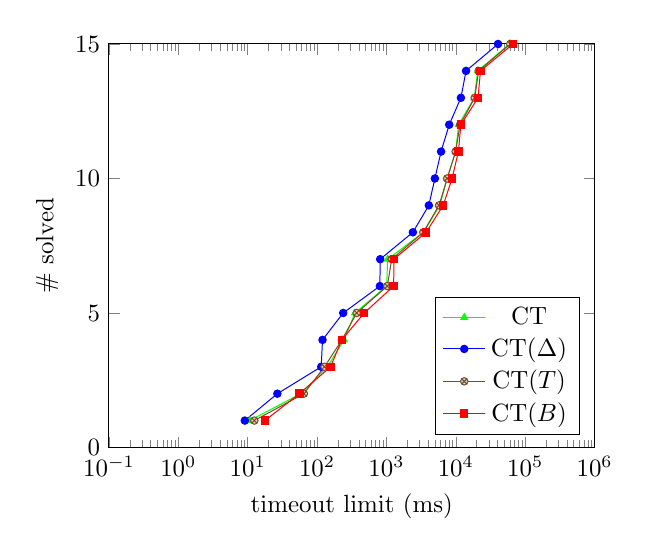
\begin{tikzpicture}[scale=0.9]
        \begin{axis}[
    xmode=log,
    ymin=0,ymax=15,
    xmin=0.1, xmax=1000000,
    every axis plot/.style={thin},
    xlabel={timeout limit (ms)},
    ylabel={\# solved},
    legend pos=south east
    % table/create on use/cumulative distribution/.style={
    %   create col/expr={\pgfmathaccuma + \thisrow{f(x)}}   
    % }
    ]
    \addplot 
    [mark=triangle*,
    mark size=1.5,
    mark options={solid},
    green] 
    coordinates {(10.724, 1)
(58.141, 2)
(140.926, 3)
(244.339, 4)
(351.655, 5)
(1007.846, 6)
(1040.618, 7)
(3429.804, 8)
(5862.337, 9)
(7518.829, 10)
(9922.216, 11)
(10995.644, 12)
(18421.925, 13)
(20703.909, 14)
(59350.857, 15)};

    \addplot 
    [blue,
    mark=*,
    mark size=1.5,
    mark options={solid}]
    coordinates {(9.092, 1)
(26.766, 2)
(114.809, 3)
(119.817, 4)
(237.752, 5)
(803.879, 6)
(812.209, 7)
(2403.255, 8)
(4081.014, 9)
(4986.668, 10)
(6124.842, 11)
(8030.718, 12)
(11828.045, 13)
(14031.517, 14)
(40586.867, 15)};

    \addplot [brown!60!black,
    mark options={fill=brown!40},
    mark=otimes*,
    mark size=1.5]
    coordinates {(12.465, 1)
(64.573, 2)
(127.898, 3)
(228.109, 4)
(372.722, 5)
(1029.302, 6)
(1191.482, 7)
(3392.266, 8)
(5728.998, 9)
(7496.585, 10)
(9916.094, 11)
(11510.717, 12)
(18700.846, 13)
(21320.804, 14)
(60889.133, 15)};

    \addplot 
    [red,
    mark size=1.5,
    mark=square*]
    coordinates {(17.667, 1)
(55.690, 2)
(156.556, 3)
(226.984, 4)
(477.676, 5)
(1271.053, 6)
(1280.040, 7)
(3730.514, 8)
(6571.512, 9)
(8823.766, 10)
(10881.983, 11)
(11821.394, 12)
(20882.392, 13)
(22667.922, 14)
(66608.065, 15)};
\legend{CT,CT($\Delta$),CT($T$),CT($B$)}
  \end{axis}

    \end{tikzpicture}
    \vfill
    \caption{\textbf{TSP Quat 20}.}
    \vspace{\baselineskip}
  \end{minipage}\qquad
  \begin{minipage}[b][8cm][s]{0.45\textwidth}
    \centering
    \vfill
    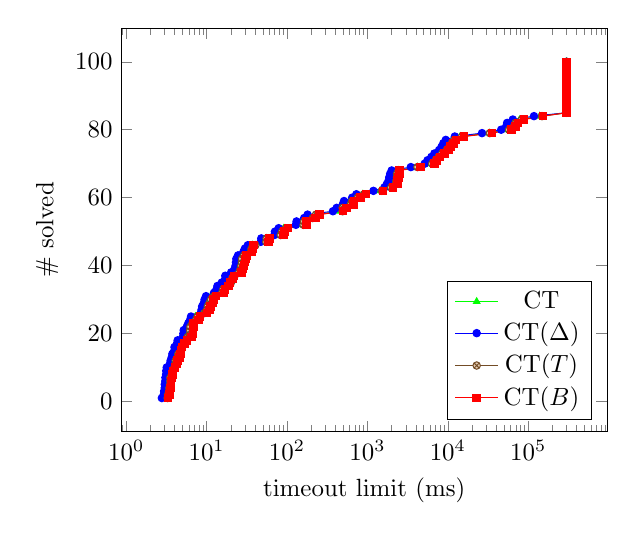
\begin{tikzpicture}[scale=0.9]
        \begin{axis}[
    xmode=log,
    every axis plot/.style={thin},
    xlabel={timeout limit (ms)},
    ylabel={\# solved},
    legend pos=south east
    % table/create on use/cumulative distribution/.style={
    %   create col/expr={\pgfmathaccuma + \thisrow{f(x)}}   
    % }
    ]
    \addplot 
    [mark=triangle*,
    mark size=1.5,
    mark options={solid},
    green] 
    coordinates {(3.196, 1)
(3.216, 2)
(3.219, 3)
(3.229, 4)
(3.236, 5)
(3.323, 6)
(3.324, 7)
(3.384, 8)
(3.555, 9)
(3.581, 10)
(3.920, 11)
(4.054, 12)
(4.316, 13)
(4.359, 14)
(4.438, 15)
(4.766, 16)
(4.899, 17)
(5.467, 18)
(5.778, 19)
(5.909, 20)
(5.980, 21)
(6.063, 22)
(6.737, 23)
(6.982, 24)
(7.263, 25)
(9.535, 26)
(9.722, 27)
(9.747, 28)
(10.539, 29)
(10.888, 30)
(11.322, 31)
(14.686, 32)
(15.476, 33)
(16.077, 34)
(17.910, 35)
(19.693, 36)
(19.701, 37)
(25.391, 38)
(25.547, 39)
(26.324, 40)
(27.363, 41)
(27.371, 42)
(28.865, 43)
(33.178, 44)
(33.245, 45)
(37.119, 46)
(53.644, 47)
(55.989, 48)
(79.967, 49)
(80.956, 50)
(91.520, 51)
(153.402, 52)
(158.352, 53)
(208.937, 54)
(228.227, 55)
(459.054, 56)
(495.212, 57)
(617.786, 58)
(634.692, 59)
(768.712, 60)
(875.114, 61)
(1437.146, 62)
(1905.669, 63)
(2114.601, 64)
(2212.913, 65)
(2220.314, 66)
(2259.432, 67)
(2410.211, 68)
(4177.779, 69)
(6168.465, 70)
(6834.469, 71)
(7334.068, 72)
(8282.489, 73)
(9512.268, 74)
(9927.672, 75)
(10947.310, 76)
(11558.129, 77)
(14232.711, 78)
(32770.476, 79)
(54494.164, 80)
(63805.832, 81)
(66673.105, 82)
(78558.979, 83)
(139323.248, 84)
(300000.148, 85)
(300000.170, 86)
(300000.230, 87)
(300000.269, 88)
(300000.313, 89)
(300000.395, 90)
(300000.426, 91)
(300000.491, 92)
(300000.615, 93)
(300000.626, 94)
(300000.663, 95)
(300000.758, 96)
(300000.834, 97)
(300000.901, 98)
(300001.161, 99)
(300001.278, 100)};

    \addplot 
    [blue,
    mark=*,
    mark size=1.5,
    mark options={solid}]
    coordinates {(2.777, 1)
(2.935, 2)
(2.962, 3)
(3.017, 4)
(3.019, 5)
(3.065, 6)
(3.077, 7)
(3.142, 8)
(3.150, 9)
(3.195, 10)
(3.490, 11)
(3.569, 12)
(3.687, 13)
(3.755, 14)
(3.975, 15)
(3.989, 16)
(4.273, 17)
(4.370, 18)
(5.066, 19)
(5.146, 20)
(5.199, 21)
(5.672, 22)
(5.925, 23)
(6.237, 24)
(6.405, 25)
(8.452, 26)
(8.651, 27)
(8.811, 28)
(9.254, 29)
(9.443, 30)
(9.845, 31)
(12.377, 32)
(13.285, 33)
(13.648, 34)
(15.465, 35)
(16.998, 36)
(17.089, 37)
(20.222, 38)
(22.259, 39)
(22.952, 40)
(23.206, 41)
(23.466, 42)
(24.612, 43)
(28.672, 44)
(29.937, 45)
(32.603, 46)
(47.179, 47)
(47.867, 48)
(69.677, 49)
(70.818, 50)
(78.794, 51)
(128.883, 52)
(131.422, 53)
(163.522, 54)
(180.337, 55)
(372.882, 56)
(414.876, 57)
(494.062, 58)
(511.910, 59)
(646.291, 60)
(729.479, 61)
(1187.909, 62)
(1627.029, 63)
(1746.098, 64)
(1833.159, 65)
(1870.757, 66)
(1917.989, 67)
(2005.271, 68)
(3468.723, 69)
(5153.090, 70)
(5590.949, 71)
(6253.125, 72)
(6807.754, 73)
(7789.728, 74)
(8368.926, 75)
(8804.268, 76)
(9432.540, 77)
(12223.062, 78)
(26637.130, 79)
(46105.675, 80)
(53283.710, 81)
(54647.876, 82)
(64363.777, 83)
(117915.726, 84)
(298513.851, 85)
(300000.155, 86)
(300000.231, 87)
(300000.251, 88)
(300000.327, 89)
(300000.341, 90)
(300000.397, 91)
(300000.468, 92)
(300000.469, 93)
(300000.508, 94)
(300000.556, 95)
(300000.575, 96)
(300000.651, 97)
(300000.702, 98)
(300000.711, 99)
(300000.912, 100)};

    \addplot [brown!60!black,
    mark options={fill=brown!40},
    mark=otimes*,
    mark size=1.5]
    coordinates {(3.271, 1)
(3.312, 2)
(3.413, 3)
(3.445, 4)
(3.513, 5)
(3.542, 6)
(3.545, 7)
(3.729, 8)
(3.847, 9)
(3.970, 10)
(4.064, 11)
(4.123, 12)
(4.357, 13)
(4.451, 14)
(4.827, 15)
(4.949, 16)
(5.189, 17)
(5.741, 18)
(5.832, 19)
(6.224, 20)
(6.239, 21)
(6.291, 22)
(6.663, 23)
(7.391, 24)
(7.727, 25)
(9.374, 26)
(10.126, 27)
(10.353, 28)
(10.850, 29)
(11.372, 30)
(12.360, 31)
(15.600, 32)
(16.099, 33)
(18.668, 34)
(20.124, 35)
(20.584, 36)
(22.324, 37)
(25.523, 38)
(26.453, 39)
(27.049, 40)
(27.494, 41)
(27.631, 42)
(29.306, 43)
(35.334, 44)
(36.200, 45)
(40.453, 46)
(55.257, 47)
(55.730, 48)
(83.536, 49)
(86.982, 50)
(96.644, 51)
(160.664, 52)
(163.689, 53)
(208.757, 54)
(229.167, 55)
(491.046, 56)
(491.402, 57)
(620.464, 58)
(644.970, 59)
(759.047, 60)
(903.670, 61)
(1512.925, 62)
(1978.608, 63)
(2256.797, 64)
(2300.228, 65)
(2328.132, 66)
(2339.827, 67)
(2441.904, 68)
(4189.045, 69)
(6398.233, 70)
(7059.747, 71)
(7672.819, 72)
(8532.069, 73)
(9683.204, 74)
(10419.366, 75)
(11199.375, 76)
(12061.647, 77)
(15029.916, 78)
(33283.823, 79)
(57881.236, 80)
(66474.073, 81)
(69399.642, 82)
(83281.381, 83)
(148458.146, 84)
(300000.162, 85)
(300000.163, 86)
(300000.270, 87)
(300000.280, 88)
(300000.298, 89)
(300000.307, 90)
(300000.316, 91)
(300000.345, 92)
(300000.405, 93)
(300000.419, 94)
(300000.420, 95)
(300000.442, 96)
(300000.548, 97)
(300000.623, 98)
(300000.805, 99)
(300001.376, 100)};

    \addplot 
    [red,
    mark size=1.5,
    mark=square*]
    coordinates {(3.316, 1)
(3.470, 2)
(3.518, 3)
(3.551, 4)
(3.592, 5)
(3.600, 6)
(3.735, 7)
(3.762, 8)
(3.816, 9)
(4.053, 10)
(4.313, 11)
(4.324, 12)
(4.630, 13)
(4.718, 14)
(4.822, 15)
(4.913, 16)
(5.339, 17)
(5.672, 18)
(6.475, 19)
(6.796, 20)
(6.800, 21)
(6.859, 22)
(6.869, 23)
(7.940, 24)
(8.327, 25)
(10.053, 26)
(10.887, 27)
(11.163, 28)
(11.941, 29)
(12.236, 30)
(13.002, 31)
(16.476, 32)
(17.063, 33)
(18.833, 34)
(19.634, 35)
(21.271, 36)
(21.980, 37)
(27.160, 38)
(28.307, 39)
(29.288, 40)
(29.853, 41)
(30.301, 42)
(31.279, 43)
(36.647, 44)
(37.576, 45)
(38.220, 46)
(59.212, 47)
(60.439, 48)
(90.691, 49)
(93.609, 50)
(102.648, 51)
(175.123, 52)
(175.969, 53)
(226.712, 54)
(251.960, 55)
(500.551, 56)
(550.919, 57)
(669.924, 58)
(681.833, 59)
(817.046, 60)
(960.972, 61)
(1559.428, 62)
(2083.045, 63)
(2366.282, 64)
(2378.071, 65)
(2435.825, 66)
(2502.688, 67)
(2505.391, 68)
(4558.792, 69)
(6832.511, 70)
(7291.945, 71)
(8012.142, 72)
(9077.137, 73)
(10207.670, 74)
(10790.878, 75)
(11695.497, 76)
(12715.296, 77)
(15991.589, 78)
(35343.944, 79)
(61685.336, 80)
(69906.557, 81)
(74635.852, 82)
(88544.807, 83)
(152679.605, 84)
(300000.253, 85)
(300000.287, 86)
(300000.324, 87)
(300000.329, 88)
(300000.332, 89)
(300000.344, 90)
(300000.345, 91)
(300000.390, 92)
(300000.398, 93)
(300000.511, 94)
(300000.522, 95)
(300000.523, 96)
(300000.694, 97)
(300000.757, 98)
(300000.769, 99)
(300001.051, 100)};
    \legend{CT,CT($\Delta$),CT($T$),CT($B$)}
  \end{axis}

    \end{tikzpicture}
    \vfill
    \caption{\textbf{Geom}.}
    \vspace{\baselineskip}
  \end{minipage}\qquad
  \begin{minipage}[b][8cm][s]{0.45\textwidth}
    \centering
    \vfill
    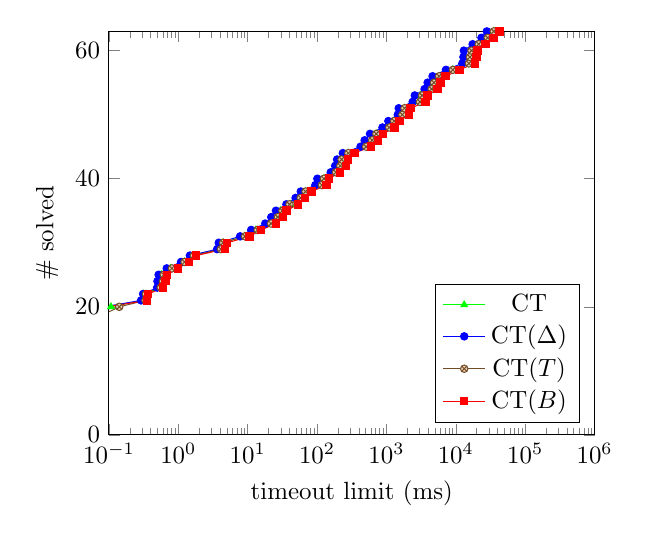
\begin{tikzpicture}[scale=0.9]
        \begin{axis}[
    xmode=log,
    ymin=0,ymax=63,
    xmin=0.1, xmax=1000000,
    every axis plot/.style={thin},
    xlabel={timeout limit (ms)},
    ylabel={\# solved},
    legend pos=south east
    % table/create on use/cumulative distribution/.style={
    %   create col/expr={\pgfmathaccuma + \thisrow{f(x)}}   
    % }
    ]
    \addplot 
    [mark=triangle*,
    mark size=1.5,
    mark options={solid},
    green] 
    coordinates {(0.061, 1)
(0.063, 2)
(0.063, 3)
(0.063, 4)
(0.066, 5)
(0.066, 6)
(0.067, 7)
(0.067, 8)
(0.068, 9)
(0.068, 10)
(0.068, 11)
(0.069, 12)
(0.069, 13)
(0.070, 14)
(0.072, 15)
(0.077, 16)
(0.077, 17)
(0.078, 18)
(0.087, 19)
(0.107, 20)
(0.302, 21)
(0.319, 22)
(0.546, 23)
(0.558, 24)
(0.571, 25)
(0.769, 26)
(1.228, 27)
(1.712, 28)
(4.017, 29)
(4.420, 30)
(8.986, 31)
(13.140, 32)
(22.686, 33)
(25.984, 34)
(29.793, 35)
(41.355, 36)
(57.374, 37)
(68.504, 38)
(120.233, 39)
(125.250, 40)
(187.928, 41)
(215.122, 42)
(239.080, 43)
(279.547, 44)
(521.134, 45)
(614.516, 46)
(709.564, 47)
(1052.148, 48)
(1307.717, 49)
(1711.958, 50)
(1808.349, 51)
(2960.202, 52)
(3082.804, 53)
(4377.795, 54)
(4793.723, 55)
(5700.589, 56)
(9022.380, 57)
(15776.713, 58)
(15978.109, 59)
(17078.488, 60)
(21737.971, 61)
(28889.226, 62)
(35570.896, 63)};

    \addplot 
    [blue,
    mark=*,
    mark size=1.5,
    mark options={solid}]
    coordinates {(0.063, 1)
(0.063, 2)
(0.064, 3)
(0.064, 4)
(0.065, 5)
(0.066, 6)
(0.066, 7)
(0.067, 8)
(0.067, 9)
(0.068, 10)
(0.070, 11)
(0.071, 12)
(0.072, 13)
(0.073, 14)
(0.077, 15)
(0.081, 16)
(0.084, 17)
(0.084, 18)
(0.084, 19)
(0.086, 20)
(0.291, 21)
(0.311, 22)
(0.496, 23)
(0.501, 24)
(0.521, 25)
(0.681, 26)
(1.096, 27)
(1.469, 28)
(3.628, 29)
(3.832, 30)
(7.775, 31)
(11.243, 32)
(17.914, 33)
(21.871, 34)
(25.542, 35)
(36.155, 36)
(48.984, 37)
(58.236, 38)
(94.364, 39)
(100.877, 40)
(157.529, 41)
(182.301, 42)
(194.176, 43)
(235.119, 44)
(423.000, 45)
(485.117, 46)
(579.516, 47)
(876.517, 48)
(1064.927, 49)
(1457.682, 50)
(1503.779, 51)
(2387.354, 52)
(2560.341, 53)
(3544.655, 54)
(3925.391, 55)
(4620.278, 56)
(7208.727, 57)
(12396.750, 58)
(12860.648, 59)
(13052.702, 60)
(17468.947, 61)
(23419.166, 62)
(27937.226, 63)};

    \addplot [brown!60!black,
    mark options={fill=brown!40},
    mark=otimes*,
    mark size=1.5]
    coordinates {(0.064, 1)
(0.064, 2)
(0.065, 3)
(0.066, 4)
(0.067, 5)
(0.067, 6)
(0.068, 7)
(0.069, 8)
(0.070, 9)
(0.071, 10)
(0.072, 11)
(0.072, 12)
(0.072, 13)
(0.072, 14)
(0.074, 15)
(0.080, 16)
(0.090, 17)
(0.090, 18)
(0.091, 19)
(0.141, 20)
(0.336, 21)
(0.342, 22)
(0.558, 23)
(0.601, 24)
(0.617, 25)
(0.809, 26)
(1.230, 27)
(1.673, 28)
(4.117, 29)
(4.428, 30)
(9.151, 31)
(13.889, 32)
(21.704, 33)
(27.173, 34)
(31.645, 35)
(40.064, 36)
(58.053, 37)
(68.236, 38)
(117.377, 39)
(125.492, 40)
(187.061, 41)
(216.572, 42)
(225.602, 43)
(282.555, 44)
(509.215, 45)
(621.611, 46)
(714.553, 47)
(1099.519, 48)
(1292.777, 49)
(1695.555, 50)
(1819.323, 51)
(3040.647, 52)
(3268.028, 53)
(4477.302, 54)
(4845.251, 55)
(5745.500, 56)
(9046.983, 57)
(15446.323, 58)
(15974.990, 59)
(16826.034, 60)
(21335.821, 61)
(28793.599, 62)
(35220.653, 63)};

    \addplot 
    [red,
    mark size=1.5,
    mark=square*]
    coordinates {(0.061, 1)
(0.062, 2)
(0.064, 3)
(0.065, 4)
(0.065, 5)
(0.066, 6)
(0.066, 7)
(0.066, 8)
(0.070, 9)
(0.070, 10)
(0.070, 11)
(0.073, 12)
(0.074, 13)
(0.074, 14)
(0.075, 15)
(0.076, 16)
(0.078, 17)
(0.078, 18)
(0.078, 19)
(0.096, 20)
(0.355, 21)
(0.368, 22)
(0.602, 23)
(0.649, 24)
(0.687, 25)
(0.990, 26)
(1.429, 27)
(1.803, 28)
(4.679, 29)
(5.060, 30)
(10.702, 31)
(15.639, 32)
(25.674, 33)
(32.030, 34)
(36.240, 35)
(53.128, 36)
(66.758, 37)
(83.306, 38)
(137.119, 39)
(147.946, 40)
(215.703, 41)
(259.463, 42)
(280.813, 43)
(344.304, 44)
(601.474, 45)
(750.007, 46)
(896.055, 47)
(1302.781, 48)
(1548.165, 49)
(2114.331, 50)
(2229.336, 51)
(3648.636, 52)
(3875.425, 53)
(5405.249, 54)
(5972.155, 55)
(7115.776, 56)
(11299.423, 57)
(18763.604, 58)
(19787.189, 59)
(20634.353, 60)
(26647.401, 61)
(35053.136, 62)
(42731.494, 63)};
    \legend{CT,CT($\Delta$),CT($T$),CT($B$)}
  \end{axis}

    \end{tikzpicture}
    \vfill
    \caption{\textbf{Crosswords LexVG}.}
    \vspace{\baselineskip}
  \end{minipage} \qquad
    \begin{minipage}[b][8cm][s]{0.45\textwidth}
    \centering
    \vfill
    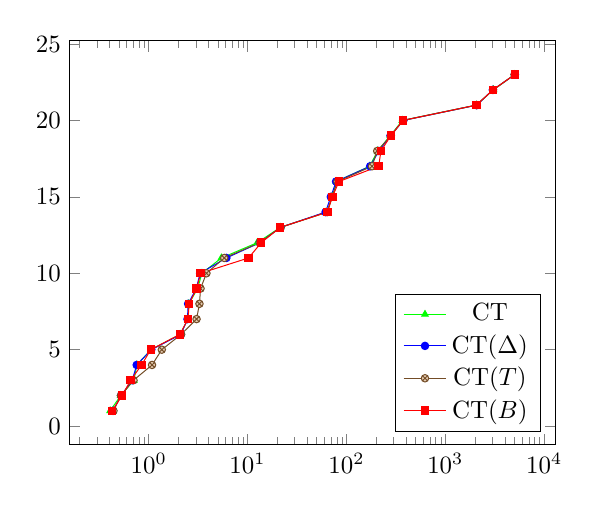
\begin{tikzpicture}[scale=0.9]
      \begin{axis}[
    xmode=log,
    every axis plot/.style={thin},
    legend pos=south east
    % table/create on use/cumulative distribution/.style={
    %   create col/expr={\pgfmathaccuma + \thisrow{f(x)}}   
    % }
    ]
    \addplot 
    [mark=triangle*,
    mark size=1.5,
    mark options={solid},
    green] 
    coordinates {
    (0.408, 1)
(0.522, 2)
(0.709, 3)
(0.760, 4)
(1.056, 5)
(2.080, 6)
(2.498, 7)
(2.545, 8)
(3.130, 9)
(3.455, 10)
(5.443, 11)
(12.540, 12)
(21.400, 13)
(63.357, 14)
(72.327, 15)
(78.959, 16)
(171.759, 17)
(206.671, 18)
(277.940, 19)
(368.226, 20)
(2055.906, 21)
(3069.686, 22)
(5042.018, 23)
    };

    \addplot 
    [blue,
    mark=*,
    mark size=1.5,
    mark options={solid}]
    coordinates {
    (0.435, 1)
(0.527, 2)
(0.682, 3)
(0.757, 4)
(1.064, 5)
(2.119, 6)
(2.471, 7)
(2.506, 8)
(3.033, 9)
(3.313, 10)
(6.107, 11)
(13.333, 12)
(21.562, 13)
(61.519, 14)
(69.514, 15)
(78.605, 16)
(173.735, 17)
(212.749, 18)
(279.236, 19)
(376.528, 20)
(2079.356, 21)
(3025.003, 22)
(5055.306, 23)
    };

    \addplot [brown!60!black,
    mark options={fill=brown!40},
    mark=otimes*,
    mark size=1.5]
    coordinates {
    (0.441, 1)
(0.524, 2)
(0.703, 3)
(1.082, 4)
(1.358, 5)
(2.130, 6)
(3.051, 7)
(3.265, 8)
(3.349, 9)
(3.843, 10)
(5.818, 11)
(13.296, 12)
(21.610, 13)
(63.892, 14)
(71.335, 15)
(81.227, 16)
(181.520, 17)
(204.798, 18)
(281.310, 19)
(374.836, 20)
(2064.777, 21)
(3039.022, 22)
(5009.530, 23)
    };

    \addplot 
    [red,
    mark size=1.5,
    mark=square*]
    coordinates {
    (0.428, 1)
(0.539, 2)
(0.658, 3)
(0.848, 4)
(1.050, 5)
(2.068, 6)
(2.501, 7)
(2.568, 8)
(3.061, 9)
(3.359, 10)
(10.237, 11)
(13.760, 12)
(21.391, 13)
(64.274, 14)
(72.091, 15)
(84.141, 16)
(211.811, 17)
(223.544, 18)
(281.354, 19)
(373.329, 20)
(2057.236, 21)
(3040.006, 22)
(5040.147, 23)
    };
    \legend{CT,CT($\Delta$),CT($T$),CT($B$)}
  \end{axis}

    \end{tikzpicture}
    \vfill
    \caption{\textbf{AIM 50}.}
    \vspace{\baselineskip}
  \end{minipage} \qquad
  
\end{figure}

\clearpage

\section{Plots from Comparison of CT against Existing Propagators}
\label{app:compare-gecode}

Each benchmark group has one figure, and each figure contains two plots:
the first plot shows for each propagator the percentage of solved instances within that group
as a function of timeout limit in milliseconds.
The second plot shows the maximum memory usage, as well as how the execution time is 
distriubted between propagation,
advisors, and copying.
For the first plot, measurements from all instances that took at least $1$~second to solve for all
propagators, and that did not cause a memory-out for any of the propagators, are included.
For the second plot, the measurements were made on one random instance within the group, such
that the runtime was at least~$10$ s for all algorithms (the accuracy of the profiling is assumed
to be too low for runtimes below~$10$ s).
For the groups of benchmarks where all instances were solved within~$10$ s for at least one algorithm,
only the memory usage is reported.
% Also, for \emph{BDD Large} and \emph{BDD Small}, no data from 

\begin{figure}
  \begin{minipage}[b][10cm][s]{0.45\textwidth}
    \centering
    \vfill
    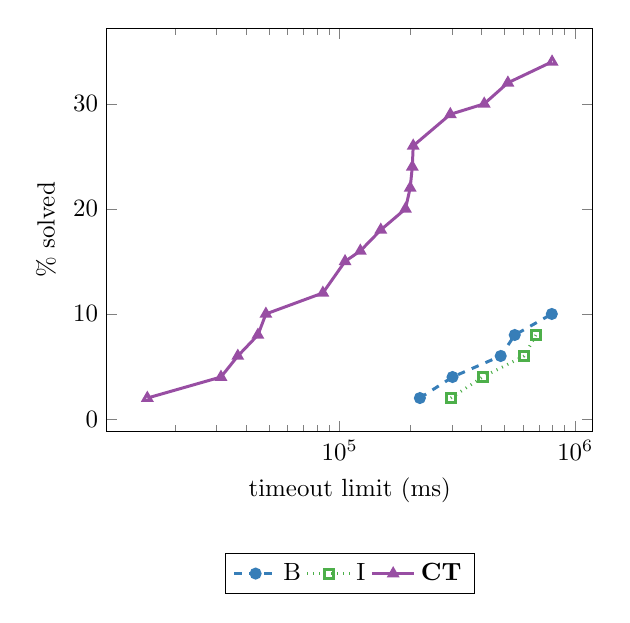
\begin{tikzpicture}[scale=0.9]
      \begin{axis}[
    xmode=log,
    every axis plot/.style={thin},
    xlabel={timeout limit (ms)},
    ylabel={\% solved},
    legend style={at={(0.5,-0.30)},
      anchor=north,legend columns=-1},
    % legend pos=south east,
    cycle list/Set1-6,
            % define fill color for the marker
            mark list fill={.!75!white},
            mark options={solid,scale=0.9},
            cycle multiindex* list={
                Set1-6
                    \nextlist
                [3 of]linestyles
                    \nextlist
                very thick
                \nextlist
                mark=o,
                mark=*,
                mark=square,
                mark=triangle,
                mark=+
            },
    ]

    \addplot
    coordinates {

    };
    \addplot
    coordinates {
      (218870, 2)
      (301170, 4)
      (482210, 6)
      (553150, 8)
      (794860, 10)

    };
    \addplot
    coordinates {
      (296190, 2)
      (404230, 4)
      (606290, 6)
      (680520, 8)

    };
    \addplot
    coordinates {
      (15250, 2)
      (31320, 4)
      (36930, 6)
      (44950, 8)
      (48590, 10)
      (84800, 12)
      (105320, 15)
      (122290, 16)
      (149390, 18)
      (190110, 20)
      (199080, 22)
      (203260, 24)
      (205030, 26)
      (294700, 29)
      (410490, 30)
      (517330, 32)
      (796770, 34)

    };


    \legend{ B, I, \textbf{CT} }
  \end{axis}

    \end{tikzpicture}
    \vspace{\baselineskip}
  \end{minipage}\qquad
  \begin{minipage}[b][10cm][s]{0.45\textwidth}
    \centering
    \vfill
    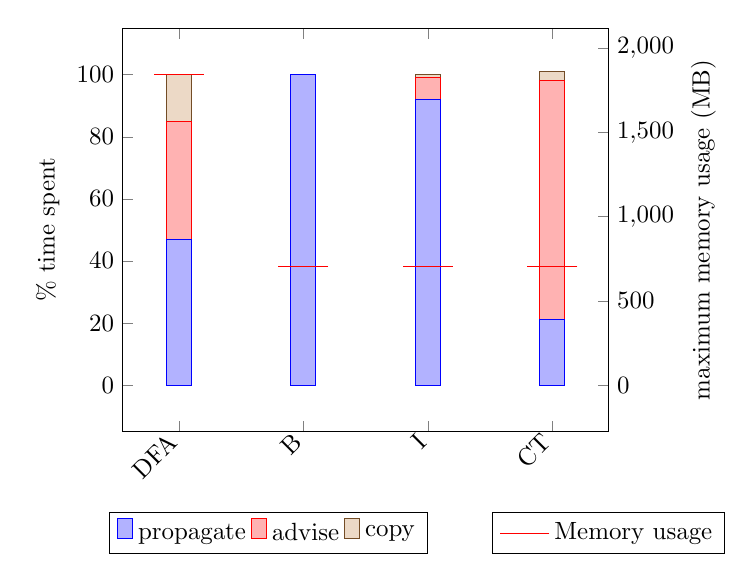
\begin{tikzpicture}[scale=0.9]
  \begin{axis}[
    ybar stacked,
    axis y line*=left,
    ymin=0,
    ymax=100,
    enlargelimits=0.15,
    legend style={at={(0.3,-0.20)},
      anchor=north,legend columns=-1},
    ylabel={\% time spent},
    symbolic x coords={DFA,B,I,CT},
    xtick=data,
    x tick label style={rotate=45,anchor=east},
    ]

    \addplot+[ybar]
      plot coordinates {
        (DFA, 47)
          (B, 100)
          (I, 92)
          (CT, 21)
          
          }; \label{ propagate }
    \addplot+[ybar]
      plot coordinates {
        (DFA, 38)
          (B, 0)
          (I, 7)
          (CT, 77)
          
          }; \label{ advise }
    \addplot+[ybar]
      plot coordinates {
        (DFA, 15)
          (B, 0)
          (I, 1)
          (CT, 3)
          
          }; \label{ copy }
    
      \legend{  }
      
      \addlegendimage{/pgfplots/refstyle=propagate}\addlegendentry{ propagate }
        
        
        \addlegendimage{/pgfplots/refstyle=advise}\addlegendentry{ advise }
        
        
        \addlegendimage{/pgfplots/refstyle=copy}\addlegendentry{ copy }
        
        
        

   \end{axis}

   \begin{axis}[
      axis y line*=right,
      axis x line=none,
      ymin=0,
      enlargelimits=0.15,
      ylabel=maximum memory usage (MB),
      legend style={at={(1.0,-0.20)},
        anchor=north,legend columns=-1},
      symbolic x coords={DFA,B,I,CT}
    ]
    \addplot+[only marks,mark size=10pt,mark=-,,mark options={.!75!red},red]
    plot coordinates {
      (DFA, 1842.919921875)
      (B, 704.638671875)
      (I, 703.1640625)
      (CT, 703.515625)
      
    };
    \addlegendentry{Memory usage}
  \end{axis}

\end{tikzpicture}

%    \vspace{\baselineskip}
  \end{minipage}\qquad
  \caption{\textbf{ A10 }}
\end{figure}
\begin{figure}[t]
  \begin{minipage}[b][10cm][s]{0.45\textwidth}
    \centering
    \vfill
    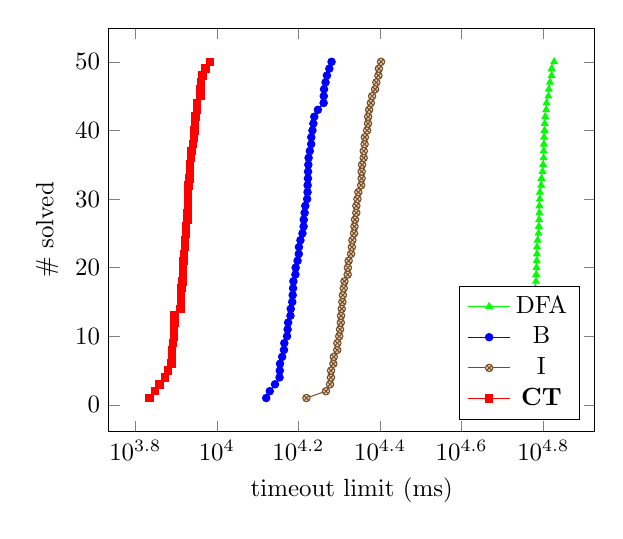
\begin{tikzpicture}[scale=0.9]
      \begin{axis}[
    xmode=log,
    every axis plot/.style={thin},
    xlabel={timeout limit (ms)},
    ylabel={\# solved},
    legend pos=south east
    % table/create on use/cumulative distribution/.style={
    %   create col/expr={\pgfmathaccuma + \thisrow{f(x)}}   
    % }
    ]
    \addplot 
    [mark=triangle*,
    mark size=1.5,
    mark options={solid},
    green] 
    coordinates {
    (51125.785, 1)
(54263.257, 2)
(56487.527, 3)
(56702.786, 4)
(56985.792, 5)
(57276.885, 6)
(57622.584, 7)
(58132.270, 8)
(58140.300, 9)
(58355.175, 10)
(58676.203, 11)
(59158.883, 12)
(59632.816, 13)
(59713.900, 14)
(59728.215, 15)
(60269.934, 16)
(60313.648, 17)
(60549.505, 18)
(60622.637, 19)
(60711.449, 20)
(60810.980, 21)
(60862.784, 22)
(60914.293, 23)
(61100.454, 24)
(61428.994, 25)
(61523.477, 26)
(61625.366, 27)
(61712.915, 28)
(61729.236, 29)
(61886.596, 30)
(61900.845, 31)
(62341.893, 32)
(62455.546, 33)
(62817.572, 34)
(63010.646, 35)
(63184.232, 36)
(63221.376, 37)
(63304.994, 38)
(63379.424, 39)
(63540.272, 40)
(63613.419, 41)
(63781.589, 42)
(64128.455, 43)
(64263.902, 44)
(64924.220, 45)
(65113.900, 46)
(65508.695, 47)
(66133.866, 48)
(66157.482, 49)
(67076.860, 50)
    };

    \addplot 
    [blue,
    mark=*,
    mark size=1.5,
    mark options={solid}]
    coordinates {
    (13210.645, 1)
(13478.699, 2)
(13880.904, 3)
(14240.906, 4)
(14262.586, 5)
(14281.012, 6)
(14453.879, 7)
(14601.257, 8)
(14630.915, 9)
(14856.229, 10)
(14906.587, 11)
(14947.426, 12)
(15147.432, 13)
(15173.599, 14)
(15300.351, 15)
(15338.350, 16)
(15370.471, 17)
(15400.162, 18)
(15575.398, 19)
(15599.555, 20)
(15767.367, 21)
(15876.487, 22)
(15890.540, 23)
(16026.936, 24)
(16207.081, 25)
(16313.213, 26)
(16328.178, 27)
(16410.911, 28)
(16468.425, 29)
(16641.910, 30)
(16678.794, 31)
(16689.212, 32)
(16716.749, 33)
(16728.322, 34)
(16755.929, 35)
(16780.814, 36)
(16896.779, 37)
(17026.619, 38)
(17037.921, 39)
(17147.387, 40)
(17237.324, 41)
(17326.549, 42)
(17685.575, 43)
(18266.956, 44)
(18281.157, 45)
(18310.293, 46)
(18466.165, 47)
(18608.783, 48)
(18864.433, 49)
(19102.683, 50)
    };

    \addplot [brown!60!black,
    mark options={fill=brown!40},
    mark=otimes*,
    mark size=1.5]
    coordinates {
    (16575.843, 1)
(18505.000, 2)
(18940.008, 3)
(19038.980, 4)
(19049.304, 5)
(19298.221, 6)
(19348.596, 7)
(19719.698, 8)
(19737.753, 9)
(19947.661, 10)
(20036.932, 11)
(20122.714, 12)
(20152.397, 13)
(20232.116, 14)
(20302.198, 15)
(20360.843, 16)
(20458.853, 17)
(20543.247, 18)
(20924.864, 19)
(20941.580, 20)
(21033.055, 21)
(21323.434, 22)
(21424.912, 23)
(21488.205, 24)
(21690.524, 25)
(21732.563, 26)
(21805.424, 27)
(21961.943, 28)
(21968.175, 29)
(22103.640, 30)
(22217.515, 31)
(22576.655, 32)
(22629.332, 33)
(22640.426, 34)
(22690.290, 35)
(22898.044, 36)
(22906.588, 37)
(23018.632, 38)
(23049.661, 39)
(23346.986, 40)
(23464.371, 41)
(23482.242, 42)
(23611.320, 43)
(23844.593, 44)
(24011.531, 45)
(24420.146, 46)
(24590.635, 47)
(24882.878, 48)
(24954.062, 49)
(25252.813, 50)
    };

    \addplot 
    [red,
    mark size=1.5,
    mark=square*]
    coordinates {
    (6834.272, 1)
(7049.566, 2)
(7238.120, 3)
(7457.754, 4)
(7598.772, 5)
(7739.737, 6)
(7771.586, 7)
(7772.970, 8)
(7812.433, 9)
(7861.439, 10)
(7862.003, 11)
(7867.552, 12)
(7871.233, 13)
(8146.006, 14)
(8162.853, 15)
(8169.022, 16)
(8197.217, 17)
(8246.900, 18)
(8258.157, 19)
(8262.374, 20)
(8291.516, 21)
(8318.251, 22)
(8342.451, 23)
(8355.561, 24)
(8389.425, 25)
(8401.690, 26)
(8470.665, 27)
(8475.034, 28)
(8489.871, 29)
(8495.761, 30)
(8507.506, 31)
(8510.152, 32)
(8560.945, 33)
(8587.622, 34)
(8588.072, 35)
(8642.789, 36)
(8662.209, 37)
(8738.285, 38)
(8798.802, 39)
(8820.422, 40)
(8831.432, 41)
(8851.771, 42)
(8928.438, 43)
(8949.293, 44)
(9107.856, 45)
(9118.812, 46)
(9135.516, 47)
(9225.896, 48)
(9370.806, 49)
(9607.234, 50)
    };
    \legend{DFA,B,I,\textbf{CT}}
  \end{axis}

    \end{tikzpicture}
    \vspace{\baselineskip}
  \end{minipage}\qquad
  \begin{minipage}[b][10cm][s]{0.45\textwidth}
    \centering
    \vfill
    \input{ tba.tex }
%    \vspace{\baselineskip}
  \end{minipage}\qquad
  \caption{\textbf{ A5 }}
\end{figure}
\begin{figure}[t]
  \begin{minipage}[b][10cm][s]{0.45\textwidth}
    \centering
    \vfill
    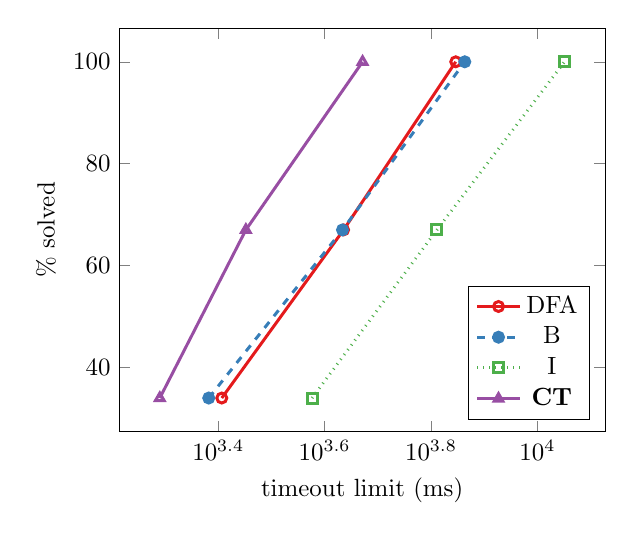
\begin{tikzpicture}[scale=0.9]
      \begin{axis}[
    xmode=log,
    every axis plot/.style={thin},
    xlabel={timeout limit (ms)},
    ylabel={\% solved},
    legend pos=south east,
    cycle list/Set1-6,
            % define fill color for the marker
            mark list fill={.!75!white},
            mark options={solid},
            cycle multiindex* list={
                Set1-6
                    \nextlist
                [3 of]linestyles
                    \nextlist
                very thick
                \nextlist
                mark=o,
                mark=*,
                mark=square,
                mark=triangle,
                mark=+
            },
    ]

    \addplot
    coordinates {
      (2550, 34)
      (4320, 67)
      (7020, 100)
      
    };
    \addplot
    coordinates {
      (2410, 34)
      (4300, 67)
      (7300, 100)
      
    };
    \addplot
    coordinates {
      (3770, 34)
      (6470, 67)
      (11240, 100)
      
    };
    \addplot
    coordinates {
      (1950, 34)
      (2830, 67)
      (4690, 100)
      
    };
    

    \legend{ DFA, B, I, \textbf{CT} }
  \end{axis}

    \end{tikzpicture}
    \vspace{\baselineskip}
  \end{minipage}\qquad
  \begin{minipage}[b][10cm][s]{0.45\textwidth}
    \centering
    \vfill
    \input{ tba.tex }
%    \vspace{\baselineskip}
  \end{minipage}\qquad
  \caption{\textbf{ AIM 50 }}
\end{figure}
\begin{figure}[t]
  \begin{minipage}[b][10cm][s]{0.45\textwidth}
    \centering
    \vfill
    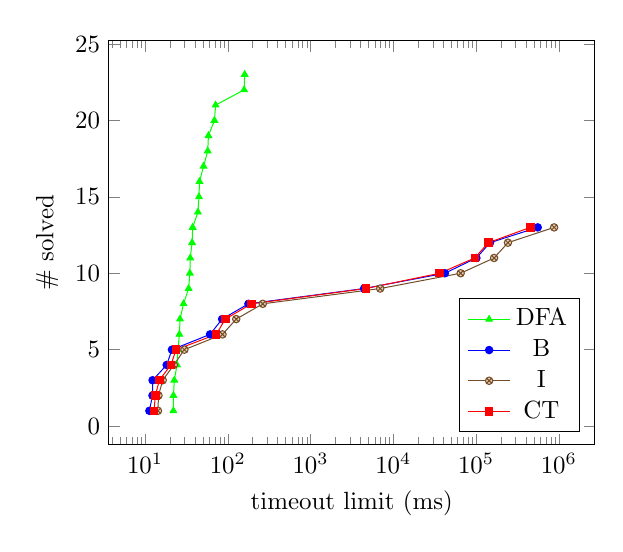
\begin{tikzpicture}[scale=0.9]
      \begin{axis}[
    xmode=log,
    every axis plot/.style={thin},
    xlabel={timeout limit (ms)},
    ylabel={\# solved},
    legend pos=south east
    % table/create on use/cumulative distribution/.style={
    %   create col/expr={\pgfmathaccuma + \thisrow{f(x)}}   
    % }
    ]
    \addplot 
    [mark=triangle*,
    mark size=1.5,
    mark options={solid},
    green] 
    coordinates {
    (21.989, 1)
(22.041, 2)
(22.559, 3)
(24.331, 4)
(24.974, 5)
(26.007, 6)
(26.462, 7)
(29.157, 8)
(33.602, 9)
(34.800, 10)
(35.158, 11)
(37.017, 12)
(37.604, 13)
(43.531, 14)
(44.847, 15)
(45.476, 16)
(50.917, 17)
(57.169, 18)
(58.349, 19)
(68.896, 20)
(71.202, 21)
(157.413, 22)
(159.802, 23)
    };

    \addplot 
    [blue,
    mark=*,
    mark size=1.5,
    mark options={solid}]
    coordinates {
    (11.281, 1)
(12.293, 2)
(12.323, 3)
(18.245, 4)
(21.125, 5)
(61.006, 6)
(85.311, 7)
(177.463, 8)
(4439.520, 9)
(41952.782, 10)
(100937.940, 11)
(147496.534, 12)
(556008.284, 13)
% (1000003.406, 14)
% (1000003.522, 15)
% (1000003.551, 16)
% (1000003.690, 17)
% (1000003.713, 18)
% (1000003.866, 19)
% (1000003.877, 20)
% (1000004.136, 21)
% (1000004.172, 22)
% (1000004.261, 23)
    };

    \addplot [brown!60!black,
    mark options={fill=brown!40},
    mark=otimes*,
    mark size=1.5]
    coordinates {
    (14.319, 1)
(14.525, 2)
(16.358, 3)
(22.251, 4)
(29.907, 5)
(86.300, 6)
(126.361, 7)
(264.396, 8)
(6937.110, 9)
(65105.320, 10)
(165084.246, 11)
(242777.983, 12)
(877449.095, 13)
% (1000004.285, 14)
% (1000004.482, 15)
% (1000004.500, 16)
% (1000004.632, 17)
% (1000004.858, 18)
% (1000004.869, 19)
% (1000004.994, 20)
% (1000015.307, 21)
% (1000021.218, 22)
% (1000094.474, 23)
    };

    \addplot 
    [red,
    mark size=1.5,
    mark=square*]
    coordinates {
    (12.839, 1)
(13.309, 2)
(14.887, 3)
(20.483, 4)
(23.742, 5)
(72.390, 6)
(93.185, 7)
(193.329, 8)
(4643.160, 9)
(36315.326, 10)
(96472.476, 11)
(140766.972, 12)
(452413.350, 13)
% (1000004.885, 14)
% (1000005.183, 15)
% (1000005.227, 16)
% (1000005.436, 17)
% (1000005.455, 18)
% (1000005.543, 19)
% (1000009.510, 20)
% (1000018.333, 21)
% (1000020.654, 22)
% (1000126.631, 23)
    };
    \legend{DFA,B,I,CT}
  \end{axis}

    \end{tikzpicture}
    \vspace{\baselineskip}
  \end{minipage}\qquad
  \begin{minipage}[b][10cm][s]{0.45\textwidth}
    \centering
    \vfill
    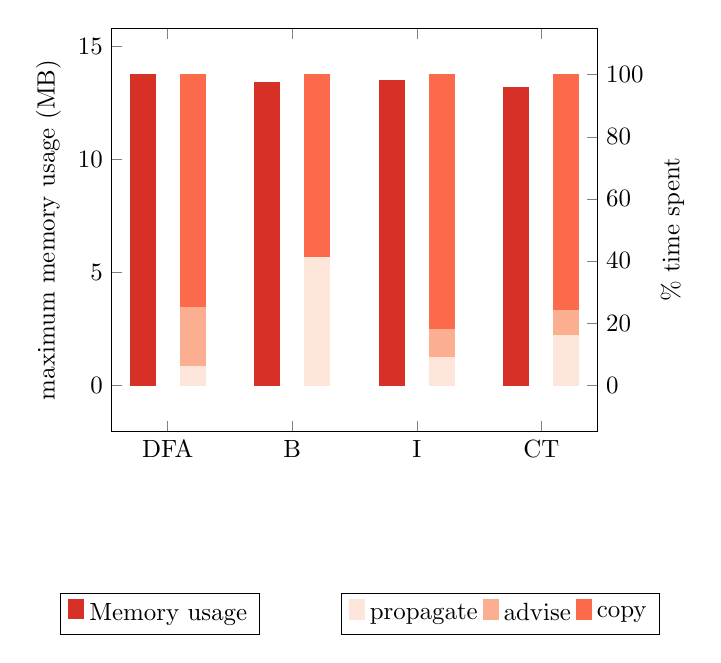
\begin{tikzpicture}[scale=0.9]
  
  \begin{axis}[
    ybar stacked,
    every axis plot/.append style={fill},
    axis y line*=left,
    ymin=0,
    enlargelimits=0.15,
    ylabel=maximum memory usage (MB),
    legend style={at={(0.1,-0.40)},
      anchor=north,legend columns=-1},
    symbolic x coords={DFA,B,I,CT},
    cycle list name=RdYlGn-9
    ]
    \addplot+[ybar,bar width=10pt,mark=none,xshift=-10pt]
    plot coordinates {
      (DFA, 13.73046875)
      (B, 13.369140625)
      (I, 13.45703125)
      (CT, 13.154296875)
      
    };
    \addlegendentry{Memory usage}
  \end{axis}

  \begin{axis}[
    ybar stacked,
    every axis plot/.append style={fill},
    axis x line=none,
    axis y line*=right,
    ymin=0,
    ymax=100,
    enlargelimits=0.15,
    legend style={at={(0.8,-0.40)},
      anchor=north,legend columns=-1},
    ylabel={\% time spent},
    symbolic x coords={DFA,B,I,CT},
    xtick=data,
    cycle list name=Reds-4,
    x tick label style={rotate=45,anchor=east},
    ]

    \addplot+[ybar,xshift=10pt]
      plot coordinates {
        (DFA, 6)
          (B, 41)
          (I, 9)
          (CT, 16)
          
          }; \label{ propagate }
    \addplot+[ybar,xshift=10pt]
      plot coordinates {
        (DFA, 19)
          (B, 0)
          (I, 9)
          (CT, 8)
          
          }; \label{ advise }
    \addplot+[ybar,xshift=10pt]
      plot coordinates {
        (DFA, 75)
          (B, 59)
          (I, 82)
          (CT, 76)
          
          }; \label{ copy }
    
      \legend{  }
      
      \addlegendimage{/pgfplots/refstyle=propagate}\addlegendentry{ propagate }
        
        \addlegendimage{/pgfplots/refstyle=advise}\addlegendentry{ advise }
        
        \addlegendimage{/pgfplots/refstyle=copy}\addlegendentry{ copy }
        
        

   \end{axis}

\end{tikzpicture}

%    \vspace{\baselineskip}
  \end{minipage}\qquad
  \caption{\textbf{ AIM 100 }}
\end{figure}
\begin{figure}[t]
  \begin{minipage}[b][10cm][s]{0.45\textwidth}
    \centering
    \vfill
    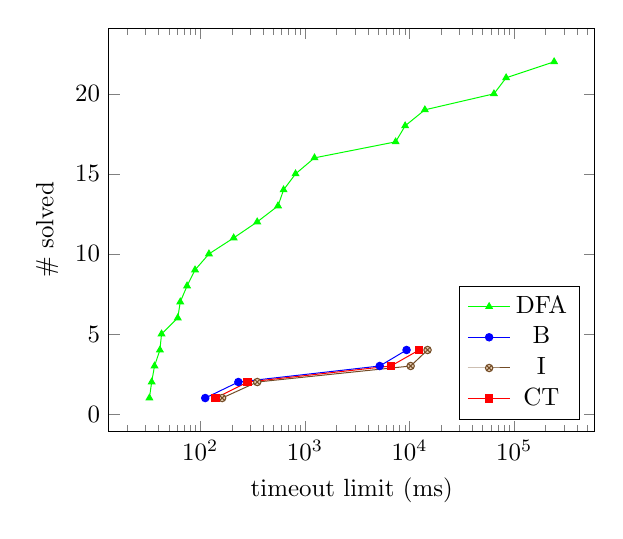
\begin{tikzpicture}[scale=0.9]
      \begin{axis}[
    xmode=log,
    every axis plot/.style={thin},
    xlabel={timeout limit (ms)},
    ylabel={\# solved},
    legend pos=south east
    % table/create on use/cumulative distribution/.style={
    %   create col/expr={\pgfmathaccuma + \thisrow{f(x)}}   
    % }
    ]
    \addplot 
    [mark=triangle*,
    mark size=1.5,
    mark options={solid},
    green] 
    coordinates {
    (32.646, 1)
(34.322, 2)
(36.539, 3)
(41.139, 4)
(42.637, 5)
(60.923, 6)
(64.362, 7)
(74.768, 8)
(89.108, 9)
(121.012, 10)
(208.525, 11)
(350.032, 12)
(553.291, 13)
(625.153, 14)
(813.725, 15)
(1234.205, 16)
(7361.018, 17)
(9076.992, 18)
(14005.709, 19)
(64038.325, 20)
(83738.459, 21)
(240798.763, 22)
    };

    \addplot 
    [blue,
    mark=*,
    mark size=1.5,
    mark options={solid}]
    coordinates {
    (111.532, 1)
(231.223, 2)
(5185.609, 3)
(9363.587, 4)
% (1000006.135, 5)
% (1000006.157, 6)
% (1000006.188, 7)
% (1000006.300, 8)
% (1000006.306, 9)
% (1000007.024, 10)
% (1000007.087, 11)
% (1000007.302, 12)
% (1000007.563, 13)
% (1000010.560, 14)
% (1000010.850, 15)
% (1000046.435, 16)
% (1000167.771, 17)
% (1001173.564, 18)
% (1006453.700, 19)
% (1008543.597, 20)
% (1010562.071, 21)
% (1019241.202, 22)
    };

    \addplot [brown!60!black,
    mark options={fill=brown!40},
    mark=otimes*,
    mark size=1.5]
    coordinates {
    (161.801, 1)
(350.376, 2)
(10244.105, 3)
(14856.666, 4)
% (1000007.483, 5)
% (1000007.625, 6)
% (1000007.695, 7)
% (1000008.729, 8)
% (1000009.950, 9)
% (1000011.262, 10)
% (1000019.536, 11)
% (1000023.192, 12)
% (1000025.767, 13)
% (1000040.365, 14)
% (1000041.636, 15)
% (1000051.012, 16)
% (1000053.849, 17)
% (1000118.768, 18)
% (1000166.508, 19)
% (1000467.387, 20)
% (1001776.595, 21)
% (1015356.678, 22)
    };

    \addplot 
    [red,
    mark size=1.5,
    mark=square*]
    coordinates {
    (140.045, 1)
(284.098, 2)
(6638.875, 3)
(12352.151, 4)
% (1000007.437, 5)
% (1000007.976, 6)
% (1000009.059, 7)
% (1000009.398, 8)
% (1000009.787, 9)
% (1000013.785, 10)
% (1000024.236, 11)
% (1000038.306, 12)
% (1000061.649, 13)
% (1000067.115, 14)
% (1000073.775, 15)
% (1000110.045, 16)
% (1000202.940, 17)
% (1000283.824, 18)
% (1001241.998, 19)
% (1012931.719, 20)
% (1016410.000, 21)
% (1021392.559, 22)
    };
    \legend{DFA,B,I,CT}
  \end{axis}

    \end{tikzpicture}
    \vspace{\baselineskip}
  \end{minipage}\qquad
  \begin{minipage}[b][10cm][s]{0.45\textwidth}
    \centering
    \vfill
    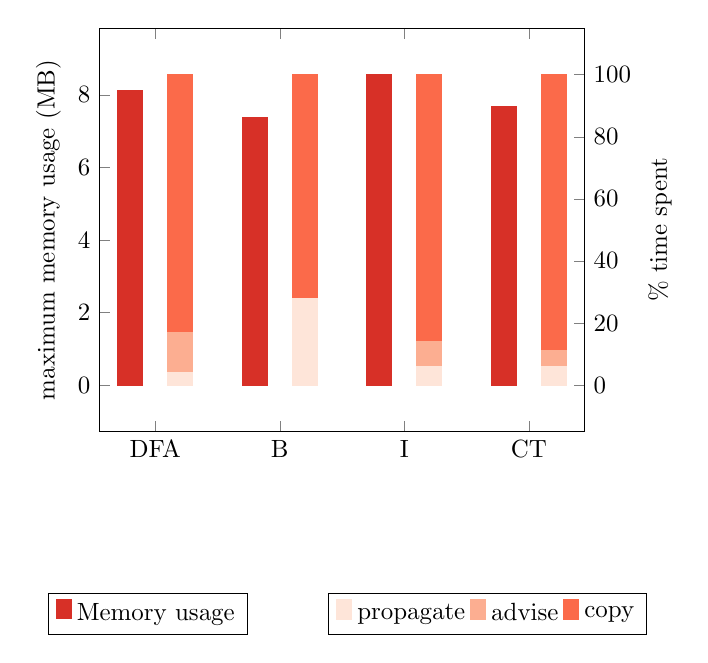
\begin{tikzpicture}[scale=0.9]
  
  \begin{axis}[
    ybar stacked,
    every axis plot/.append style={fill},
    axis y line*=left,
    ymin=0,
    enlargelimits=0.15,
    ylabel=maximum memory usage (MB),
    legend style={at={(0.1,-0.40)},
      anchor=north,legend columns=-1},
    symbolic x coords={DFA,B,I,CT},
    cycle list name=RdYlGn-9
    ]
    \addplot+[ybar,bar width=10pt,mark=none,xshift=-10pt]
    plot coordinates {
      (DFA, 8.115234375)
      (B, 7.373046875)
      (I, 8.5546875)
      (CT, 7.685546875)
      
    };
    \addlegendentry{Memory usage}
  \end{axis}

  \begin{axis}[
    ybar stacked,
    every axis plot/.append style={fill},
    axis x line=none,
    axis y line*=right,
    ymin=0,
    ymax=100,
    enlargelimits=0.15,
    legend style={at={(0.8,-0.40)},
      anchor=north,legend columns=-1},
    ylabel={\% time spent},
    symbolic x coords={DFA,B,I,CT},
    xtick=data,
    cycle list name=Reds-4,
    x tick label style={rotate=45,anchor=east},
    ]

    \addplot+[ybar,xshift=10pt]
      plot coordinates {
        (DFA, 4)
          (B, 28)
          (I, 6)
          (CT, 6)
          
          }; \label{ propagate }
    \addplot+[ybar,xshift=10pt]
      plot coordinates {
        (DFA, 13)
          (B, 0)
          (I, 8)
          (CT, 5)
          
          }; \label{ advise }
    \addplot+[ybar,xshift=10pt]
      plot coordinates {
        (DFA, 83)
          (B, 72)
          (I, 86)
          (CT, 89)
          
          }; \label{ copy }
    
      \legend{  }
      
      \addlegendimage{/pgfplots/refstyle=propagate}\addlegendentry{ propagate }
        
        \addlegendimage{/pgfplots/refstyle=advise}\addlegendentry{ advise }
        
        \addlegendimage{/pgfplots/refstyle=copy}\addlegendentry{ copy }
        
        

   \end{axis}

\end{tikzpicture}

%    \vspace{\baselineskip}
  \end{minipage}\qquad
  \caption{\textbf{ AIM 200 }}
\end{figure}
\begin{figure}[t]
  \begin{minipage}[b][10cm][s]{0.45\textwidth}
    \centering
    \vfill
    \begin{tikzpicture}[scale=0.9]
      \begin{axis}[
    xmode=log,
    every axis plot/.style={thin},
    xlabel={timeout limit (ms)},
    ylabel={\% solved},
    legend style={at={(0.5,-0.30)},
      anchor=north,legend columns=-1},
    % legend pos=south east,
    cycle list/Set1-6,
            % define fill color for the marker
            mark list fill={.!75!white},
            mark options={solid,scale=0.9},
            cycle multiindex* list={
                Set1-6
                    \nextlist
                [3 of]linestyles
                    \nextlist
                very thick
                \nextlist
                mark=o,
                mark=*,
                mark=square,
                mark=triangle,
                mark=+
            },
    ]

    

    \legend{ DFA, B, I, \textbf{CT} }
  \end{axis}

    \end{tikzpicture}
    \vspace{\baselineskip}
  \end{minipage}\qquad
  \begin{minipage}[b][10cm][s]{0.45\textwidth}
    \centering
    \vfill
    \input{ tba.tex }
%    \vspace{\baselineskip}
  \end{minipage}\qquad
  \caption{\textbf{ BDD Small }}
\end{figure}
\begin{figure}[t]
  \begin{minipage}[b][10cm][s]{0.45\textwidth}
    \centering
    \vfill
    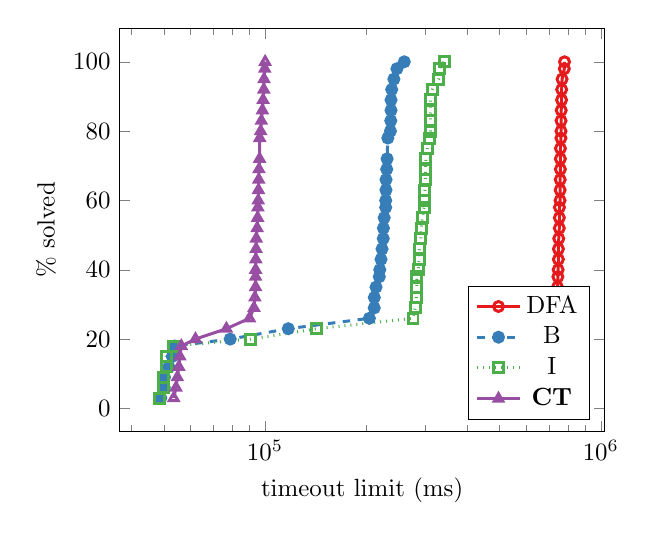
\begin{tikzpicture}[scale=0.9]
      \begin{axis}[
    xmode=log,
    every axis plot/.style={thin},
    xlabel={timeout limit (ms)},
    ylabel={\% solved},
    legend pos=south east,
    cycle list/Set1-6,
            % define fill color for the marker
            mark list fill={.!75!white},
            mark options={solid},
            cycle multiindex* list={
                Set1-6
                    \nextlist
                [3 of]linestyles
                    \nextlist
                very thick
                \nextlist
                mark=o,
                mark=*,
                mark=square,
                mark=triangle,
                mark=+
            },
    ]

    \addplot
    coordinates {
      (663310, 3)
      (668120, 6)
      (674240, 9)
      (681210, 12)
      (682080, 15)
      (693360, 18)
      (701800, 20)
      (710510, 23)
      (721370, 26)
      (733270, 29)
      (737690, 32)
      (743100, 35)
      (744950, 38)
      (746390, 40)
      (747580, 43)
      (747780, 46)
      (749520, 49)
      (752380, 52)
      (752460, 55)
      (752970, 58)
      (756240, 60)
      (756590, 63)
      (757070, 66)
      (757940, 69)
      (757950, 72)
      (758210, 75)
      (760950, 78)
      (761150, 80)
      (761270, 83)
      (762350, 86)
      (764150, 89)
      (764630, 92)
      (766660, 95)
      (778590, 98)
      (779820, 100)
      
    };
    \addplot
    coordinates {
      (48960, 3)
      (50130, 6)
      (50220, 9)
      (51730, 12)
      (52950, 15)
      (53810, 18)
      (78780, 20)
      (117310, 23)
      (204580, 26)
      (211480, 29)
      (211610, 32)
      (214100, 35)
      (218950, 38)
      (219710, 40)
      (221560, 43)
      (223130, 46)
      (225000, 49)
      (225250, 52)
      (226390, 55)
      (228770, 58)
      (228800, 60)
      (229210, 63)
      (229280, 66)
      (230400, 69)
      (230980, 72)
      (232150, 78)
      (236310, 80)
      (236880, 83)
      (237290, 86)
      (237320, 89)
      (238430, 92)
      (242000, 95)
      (247080, 98)
      (259880, 100)
      
    };
    \addplot
    coordinates {
      (48610, 3)
      (49700, 6)
      (49990, 9)
      (50810, 12)
      (51050, 15)
      (53250, 18)
      (90540, 20)
      (142650, 23)
      (275900, 26)
      (280260, 29)
      (282090, 32)
      (283200, 35)
      (283420, 38)
      (285910, 40)
      (287700, 43)
      (288220, 46)
      (291090, 49)
      (291560, 52)
      (294120, 55)
      (297560, 58)
      (297750, 60)
      (299160, 63)
      (300220, 66)
      (300620, 69)
      (301270, 72)
      (304330, 75)
      (308970, 78)
      (310620, 80)
      (310750, 83)
      (310990, 86)
      (311140, 89)
      (315640, 92)
      (328920, 95)
      (329910, 98)
      (341360, 100)
      
    };
    \addplot
    coordinates {
      (53490, 3)
      (54330, 6)
      (54840, 9)
      (55390, 12)
      (55780, 15)
      (56350, 18)
      (62080, 20)
      (76760, 23)
      (89920, 26)
      (92730, 29)
      (93300, 32)
      (93750, 35)
      (93760, 38)
      (93770, 40)
      (93910, 43)
      (94080, 46)
      (94190, 49)
      (94750, 52)
      (95060, 55)
      (95240, 58)
      (95480, 60)
      (95620, 63)
      (95790, 66)
      (95950, 69)
      (96350, 72)
      (96460, 78)
      (97070, 80)
      (97530, 83)
      (98260, 86)
      (98700, 89)
      (99170, 92)
      (99350, 95)
      (99830, 98)
      (100100, 100)
      
    };
    

    \legend{ DFA, B, I, \textbf{CT} }
  \end{axis}

    \end{tikzpicture}
    \vspace{\baselineskip}
  \end{minipage}\qquad
  \begin{minipage}[b][10cm][s]{0.45\textwidth}
    \centering
    \vfill
    \input{ tba.tex }
%    \vspace{\baselineskip}
  \end{minipage}\qquad
  \caption{\textbf{ BDD Large }}
\end{figure}
\begin{figure}[t]
  \begin{minipage}[b][10cm][s]{0.45\textwidth}
    \centering
    \vfill
    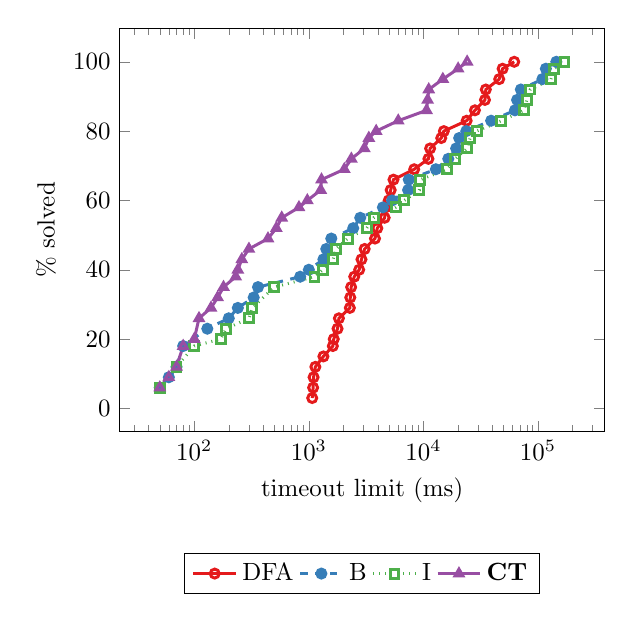
\begin{tikzpicture}[scale=0.9]
      \begin{axis}[
    xmode=log,
    every axis plot/.style={thin},
    xlabel={timeout limit (ms)},
    ylabel={\% solved},
    legend style={at={(0.5,-0.30)},
      anchor=north,legend columns=-1},
    % legend pos=south east,
    cycle list/Set1-6,
            % define fill color for the marker
            mark list fill={.!75!white},
            mark options={solid,scale=0.9},
            cycle multiindex* list={
                Set1-6
                    \nextlist
                [3 of]linestyles
                    \nextlist
                very thick
                \nextlist
                mark=o,
                mark=*,
                mark=square,
                mark=triangle,
                mark=+
            },
    ]

    \addplot
    coordinates {
      (1070, 3)
      (1090, 6)
      (1100, 9)
      (1140, 12)
      (1340, 15)
      (1620, 18)
      (1650, 20)
      (1780, 23)
      (1830, 26)
      (2280, 29)
      (2300, 32)
      (2340, 35)
      (2490, 38)
      (2750, 40)
      (2880, 43)
      (3070, 46)
      (3780, 49)
      (3960, 52)
      (4590, 55)
      (4680, 58)
      (4980, 60)
      (5180, 63)
      (5480, 66)
      (8310, 69)
      (11060, 72)
      (11440, 75)
      (14310, 78)
      (15080, 80)
      (23840, 83)
      (28160, 86)
      (34450, 89)
      (35060, 92)
      (45870, 95)
      (49120, 98)
      (62030, 100)
      
    };
    \addplot
    coordinates {
      (50, 6)
      (60, 9)
      (70, 12)
      (80, 18)
      (130, 23)
      (200, 26)
      (240, 29)
      (330, 32)
      (360, 35)
      (840, 38)
      (1000, 40)
      (1340, 43)
      (1420, 46)
      (1570, 49)
      (2440, 52)
      (2810, 55)
      (4430, 58)
      (5330, 60)
      (7350, 63)
      (7450, 66)
      (12850, 69)
      (16490, 72)
      (19310, 75)
      (20520, 78)
      (23670, 80)
      (39020, 83)
      (62930, 86)
      (65710, 89)
      (70870, 92)
      (109260, 95)
      (117110, 98)
      (144570, 100)
      
    };
    \addplot
    coordinates {
      (50, 6)
      (70, 12)
      (100, 18)
      (170, 20)
      (190, 23)
      (300, 26)
      (320, 29)
      (500, 35)
      (1120, 38)
      (1330, 40)
      (1630, 43)
      (1720, 46)
      (2180, 49)
      (3200, 52)
      (3680, 55)
      (5710, 58)
      (6810, 60)
      (9230, 63)
      (9390, 66)
      (16190, 69)
      (18960, 72)
      (24090, 75)
      (25580, 78)
      (29300, 80)
      (47970, 83)
      (75460, 86)
      (80010, 89)
      (85710, 92)
      (129810, 95)
      (138470, 98)
      (170370, 100)
      
    };
    \addplot
    coordinates {
      (50, 6)
      (60, 9)
      (70, 12)
      (80, 18)
      (100, 20)
      (110, 26)
      (140, 29)
      (160, 32)
      (180, 35)
      (230, 38)
      (240, 40)
      (260, 43)
      (300, 46)
      (440, 49)
      (520, 52)
      (580, 55)
      (820, 58)
      (970, 60)
      (1270, 63)
      (1290, 66)
      (2040, 69)
      (2350, 72)
      (3050, 75)
      (3340, 78)
      (3870, 80)
      (6030, 83)
      (10650, 86)
      (10890, 89)
      (11130, 92)
      (14780, 95)
      (20090, 98)
      (24080, 100)
      
    };
    

    \legend{ DFA, B, I, \textbf{CT} }
  \end{axis}

    \end{tikzpicture}
    \vspace{\baselineskip}
  \end{minipage}\qquad
  \begin{minipage}[b][10cm][s]{0.45\textwidth}
    \centering
    \vfill
    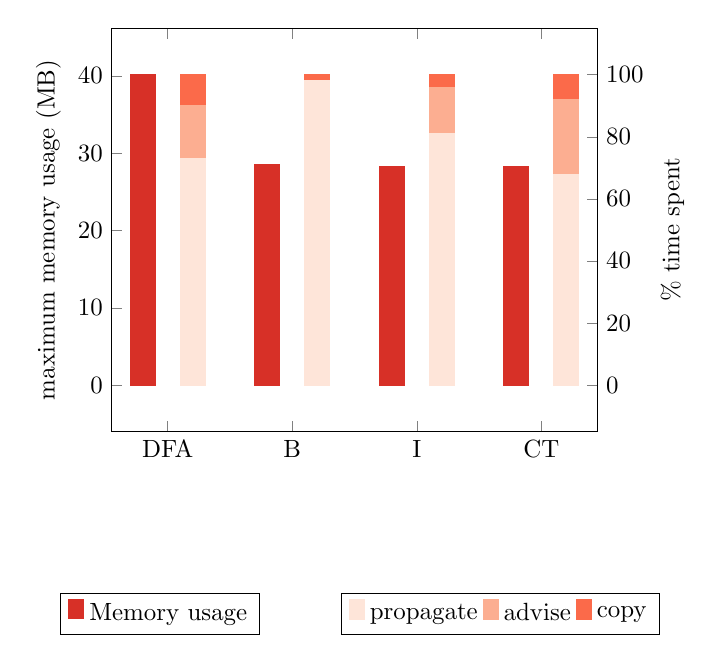
\begin{tikzpicture}[scale=0.9]
  
  \begin{axis}[
    ybar stacked,
    every axis plot/.append style={fill},
    axis y line*=left,
    ymin=0,
    enlargelimits=0.15,
    ylabel=maximum memory usage (MB),
    legend style={at={(0.1,-0.40)},
      anchor=north,legend columns=-1},
    symbolic x coords={DFA,B,I,CT},
    cycle list name=RdYlGn-9
    ]
    \addplot+[ybar,bar width=10pt,mark=none,xshift=-10pt]
    plot coordinates {
      (DFA, 40.15625)
      (B, 28.49609375)
      (I, 28.310546875)
      (CT, 28.30078125)
      
    };
    \addlegendentry{Memory usage}
  \end{axis}

  \begin{axis}[
    ybar stacked,
    every axis plot/.append style={fill},
    axis x line=none,
    axis y line*=right,
    ymin=0,
    ymax=100,
    enlargelimits=0.15,
    legend style={at={(0.8,-0.40)},
      anchor=north,legend columns=-1},
    ylabel={\% time spent},
    symbolic x coords={DFA,B,I,CT},
    xtick=data,
    cycle list name=Reds-4,
    x tick label style={rotate=45,anchor=east},
    ]

    \addplot+[ybar,xshift=10pt]
      plot coordinates {
        (DFA, 73)
          (B, 98)
          (I, 81)
          (CT, 68)
          
          }; \label{ propagate }
    \addplot+[ybar,xshift=10pt]
      plot coordinates {
        (DFA, 17)
          (B, 0)
          (I, 15)
          (CT, 24)
          
          }; \label{ advise }
    \addplot+[ybar,xshift=10pt]
      plot coordinates {
        (DFA, 10)
          (B, 2)
          (I, 4)
          (CT, 8)
          
          }; \label{ copy }
    
      \legend{  }
      
      \addlegendimage{/pgfplots/refstyle=propagate}\addlegendentry{ propagate }
        
        \addlegendimage{/pgfplots/refstyle=advise}\addlegendentry{ advise }
        
        \addlegendimage{/pgfplots/refstyle=copy}\addlegendentry{ copy }
        
        

   \end{axis}

\end{tikzpicture}

%    \vspace{\baselineskip}
  \end{minipage}\qquad
  \caption{\textbf{ Crosswords lexVg }}
\end{figure}
\begin{figure}[t]
  \begin{minipage}[b][10cm][s]{0.45\textwidth}
    \centering
    \vfill
    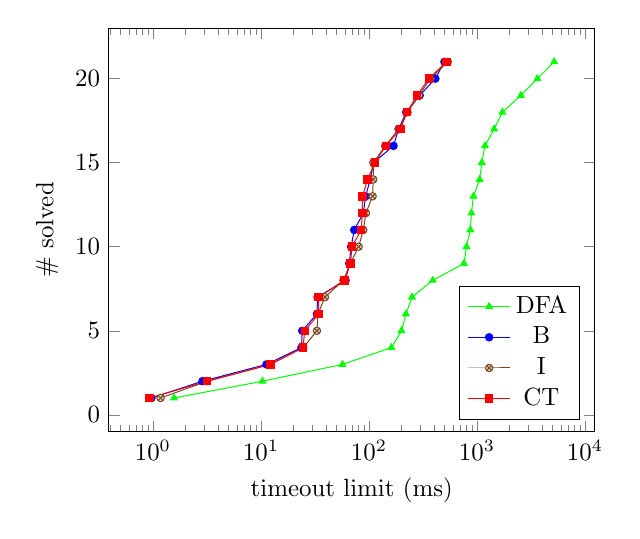
\begin{tikzpicture}[scale=0.9]
      \begin{axis}[
    xmode=log,
    every axis plot/.style={thin},
    xlabel={timeout limit (ms)},
    ylabel={\# solved},
    legend pos=south east
    % table/create on use/cumulative distribution/.style={
    %   create col/expr={\pgfmathaccuma + \thisrow{f(x)}}   
    % }
    ]
    \addplot 
    [mark=triangle*,
    mark size=1.5,
    mark options={solid},
    green] 
    coordinates {
(1.569, 1)
(10.341, 2)
(56.930, 3)
(161.466, 4)
(200.271, 5)
(220.150, 6)
(250.496, 7)
(389.479, 8)
(757.830, 9)
(800.580, 10)
(868.873, 11)
(888.415, 12)
(928.329, 13)
(1059.826, 14)
(1108.592, 15)
(1186.171, 16)
(1442.143, 17)
(1718.117, 18)
(2549.019, 19)
(3626.036, 20)
(5178.601, 21)
    };

    \addplot 
    [blue,
    mark=*,
    mark size=1.5,
    mark options={solid}]
    coordinates {
(0.969, 1)
(2.881, 2)
(11.268, 3)
(23.734, 4)
(24.138, 5)
(33.016, 6)
(33.480, 7)
(60.819, 8)
(65.730, 9)
(68.464, 10)
(73.136, 11)
(88.944, 12)
(92.941, 13)
(103.030, 14)
(110.307, 15)
(168.815, 16)
(188.304, 17)
(221.341, 18)
(295.291, 19)
(412.154, 20)
(499.695, 21)
    };

    \addplot [brown!60!black,
    mark options={fill=brown!40},
    mark=otimes*,
    mark size=1.5]
    coordinates {
(1.178, 1)
(3.182, 2)
(12.190, 3)
(24.682, 4)
(33.012, 5)
(33.778, 6)
(39.197, 7)
(58.045, 8)
(67.182, 9)
(80.311, 10)
(88.742, 11)
(93.862, 12)
(108.193, 13)
(109.575, 14)
(110.207, 15)
(141.416, 16)
(189.383, 17)
(227.490, 18)
(289.981, 19)
(370.487, 20)
(537.222, 21)
    };

    \addplot 
    [red,
    mark size=1.5,
    mark=square*]
    coordinates {
(0.929, 1)
(3.171, 2)
(12.289, 3)
(24.504, 4)
(25.467, 5)
(34.223, 6)
(34.294, 7)
(59.192, 8)
(67.660, 9)
(69.445, 10)
(84.905, 11)
(86.923, 12)
(87.166, 13)
(97.317, 14)
(113.314, 15)
(143.394, 16)
(195.333, 17)
(225.252, 18)
(279.125, 19)
(358.324, 20)
(525.028, 21)
    };
    \legend{DFA,B,I,CT}
  \end{axis}

    \end{tikzpicture}
    \vspace{\baselineskip}
  \end{minipage}\qquad
  \begin{minipage}[b][10cm][s]{0.45\textwidth}
    \centering
    \vfill
    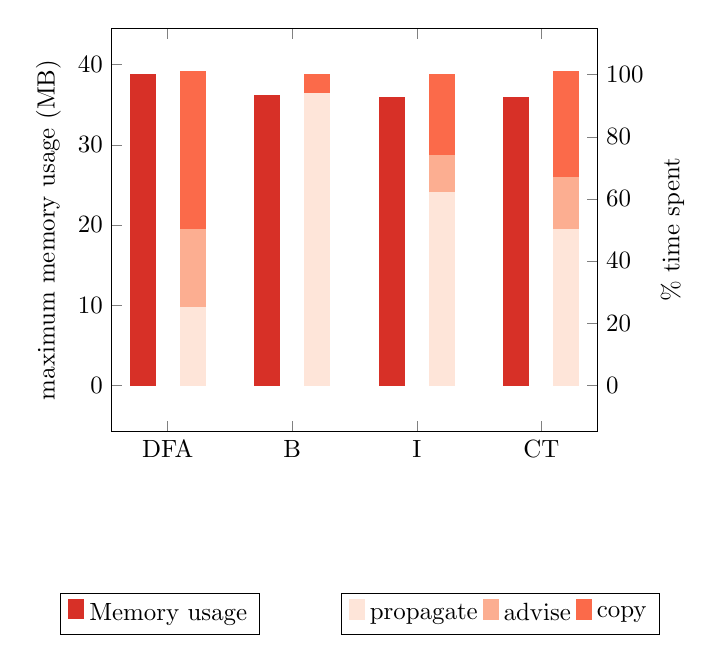
\begin{tikzpicture}[scale=0.9]
  
  \begin{axis}[
    ybar stacked,
    every axis plot/.append style={fill},
    axis y line*=left,
    ymin=0,
    enlargelimits=0.15,
    ylabel=maximum memory usage (MB),
    legend style={at={(0.1,-0.40)},
      anchor=north,legend columns=-1},
    symbolic x coords={DFA,B,I,CT},
    cycle list name=RdYlGn-9
    ]
    \addplot+[ybar,bar width=10pt,mark=none,xshift=-10pt]
    plot coordinates {
      (DFA, 38.75)
      (B, 36.1328125)
      (I, 35.9375)
      (CT, 35.8984375)
      
    };
    \addlegendentry{Memory usage}
  \end{axis}

  \begin{axis}[
    ybar stacked,
    every axis plot/.append style={fill},
    axis x line=none,
    axis y line*=right,
    ymin=0,
    ymax=100,
    enlargelimits=0.15,
    legend style={at={(0.8,-0.40)},
      anchor=north,legend columns=-1},
    ylabel={\% time spent},
    symbolic x coords={DFA,B,I,CT},
    xtick=data,
    cycle list name=Reds-4,
    x tick label style={rotate=45,anchor=east},
    ]

    \addplot+[ybar,xshift=10pt]
      plot coordinates {
        (DFA, 25)
          (B, 94)
          (I, 62)
          (CT, 50)
          
          }; \label{ propagate }
    \addplot+[ybar,xshift=10pt]
      plot coordinates {
        (DFA, 25)
          (B, 0)
          (I, 12)
          (CT, 17)
          
          }; \label{ advise }
    \addplot+[ybar,xshift=10pt]
      plot coordinates {
        (DFA, 51)
          (B, 6)
          (I, 26)
          (CT, 34)
          
          }; \label{ copy }
    
      \legend{  }
      
      \addlegendimage{/pgfplots/refstyle=propagate}\addlegendentry{ propagate }
        
        \addlegendimage{/pgfplots/refstyle=advise}\addlegendentry{ advise }
        
        \addlegendimage{/pgfplots/refstyle=copy}\addlegendentry{ copy }
        
        

   \end{axis}

\end{tikzpicture}

%    \vspace{\baselineskip}
  \end{minipage}\qquad
  \caption{\textbf{ Crosswords wordsPuzzle }}
\end{figure}
\begin{figure}[t]
  \begin{minipage}[b][10cm][s]{0.45\textwidth}
    \centering
    \vfill
    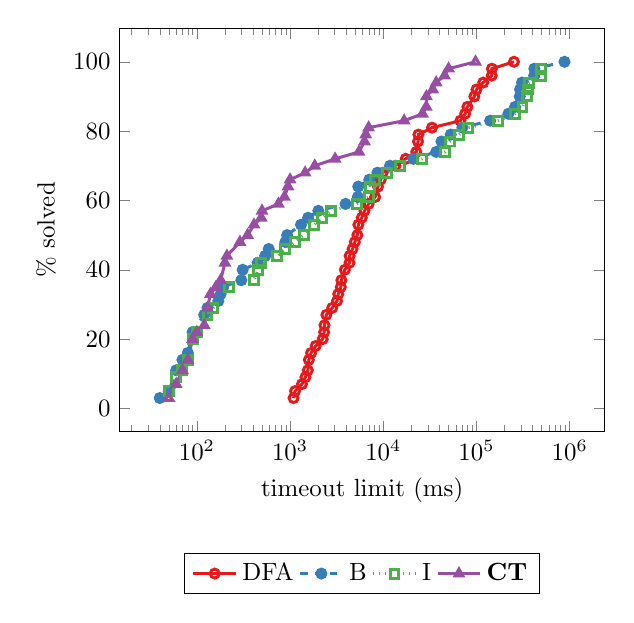
\begin{tikzpicture}[scale=0.9]
      \begin{axis}[
    xmode=log,
    every axis plot/.style={thin},
    xlabel={timeout limit (ms)},
    ylabel={\% solved},
    legend style={at={(0.5,-0.30)},
      anchor=north,legend columns=-1},
    % legend pos=south east,
    cycle list/Set1-6,
            % define fill color for the marker
            mark list fill={.!75!white},
            mark options={solid,scale=0.9},
            cycle multiindex* list={
                Set1-6
                    \nextlist
                [3 of]linestyles
                    \nextlist
                very thick
                \nextlist
                mark=o,
                mark=*,
                mark=square,
                mark=triangle,
                mark=+
            },
    ]

    \addplot
    coordinates {
      (1090, 3)
      (1130, 5)
      (1340, 7)
      (1460, 9)
      (1550, 11)
      (1590, 14)
      (1680, 16)
      (1880, 18)
      (2240, 20)
      (2320, 22)
      (2340, 24)
      (2450, 27)
      (2830, 29)
      (3190, 31)
      (3290, 33)
      (3500, 35)
      (3550, 37)
      (3870, 40)
      (4340, 42)
      (4350, 44)
      (4680, 46)
      (4950, 48)
      (5270, 50)
      (5400, 53)
      (5880, 55)
      (6280, 57)
      (6960, 59)
      (8170, 61)
      (8770, 64)
      (9380, 66)
      (9840, 68)
      (13500, 70)
      (17400, 72)
      (22580, 74)
      (23570, 77)
      (23810, 79)
      (33320, 81)
      (67210, 83)
      (75510, 85)
      (79890, 87)
      (94840, 90)
      (99880, 92)
      (118040, 94)
      (145590, 96)
      (146260, 98)
      (252130, 100)
      
    };
    \addplot
    coordinates {
      (40, 3)
      (50, 5)
      (60, 11)
      (70, 14)
      (80, 16)
      (90, 22)
      (120, 27)
      (130, 29)
      (170, 31)
      (180, 33)
      (190, 35)
      (300, 37)
      (310, 40)
      (450, 42)
      (540, 44)
      (590, 46)
      (890, 48)
      (930, 50)
      (1310, 53)
      (1560, 55)
      (2010, 57)
      (3940, 59)
      (5330, 61)
      (5390, 64)
      (7080, 66)
      (8650, 68)
      (11800, 70)
      (21010, 72)
      (36960, 74)
      (42090, 77)
      (52930, 79)
      (70600, 81)
      (140070, 83)
      (219890, 85)
      (259150, 87)
      (290930, 90)
      (293180, 92)
      (307460, 94)
      (415600, 96)
      (417390, 98)
      (879060, 100)
      
    };
    \addplot
    coordinates {
      (50, 5)
      (60, 9)
      (70, 11)
      (80, 14)
      (90, 20)
      (100, 22)
      (130, 27)
      (150, 29)
      (220, 35)
      (410, 37)
      (450, 40)
      (490, 42)
      (730, 44)
      (890, 46)
      (1130, 48)
      (1400, 50)
      (1810, 53)
      (2220, 55)
      (2740, 57)
      (5190, 59)
      (6980, 61)
      (7220, 64)
      (8240, 66)
      (11030, 68)
      (15130, 70)
      (26310, 72)
      (45850, 74)
      (51450, 77)
      (65270, 79)
      (80850, 81)
      (169630, 83)
      (259520, 85)
      (311430, 87)
      (346140, 90)
      (353150, 92)
      (361750, 94)
      (492850, 96)
      (494920, 98)
      
    };
    \addplot
    coordinates {
      (50, 3)
      (60, 7)
      (70, 11)
      (80, 14)
      (90, 20)
      (100, 22)
      (120, 24)
      (130, 29)
      (140, 33)
      (160, 35)
      (180, 37)
      (200, 42)
      (210, 44)
      (290, 48)
      (350, 50)
      (410, 53)
      (490, 55)
      (500, 57)
      (750, 59)
      (870, 61)
      (950, 64)
      (1000, 66)
      (1450, 68)
      (1840, 70)
      (3040, 72)
      (5480, 74)
      (6280, 77)
      (6480, 79)
      (6970, 81)
      (16740, 83)
      (26310, 85)
      (28910, 87)
      (29020, 90)
      (33910, 92)
      (36940, 94)
      (45410, 96)
      (50170, 98)
      (97580, 100)
      
    };
    

    \legend{ DFA, B, I, \textbf{CT} }
  \end{axis}

    \end{tikzpicture}
    \vspace{\baselineskip}
  \end{minipage}\qquad
  \begin{minipage}[b][10cm][s]{0.45\textwidth}
    \centering
    \vfill
    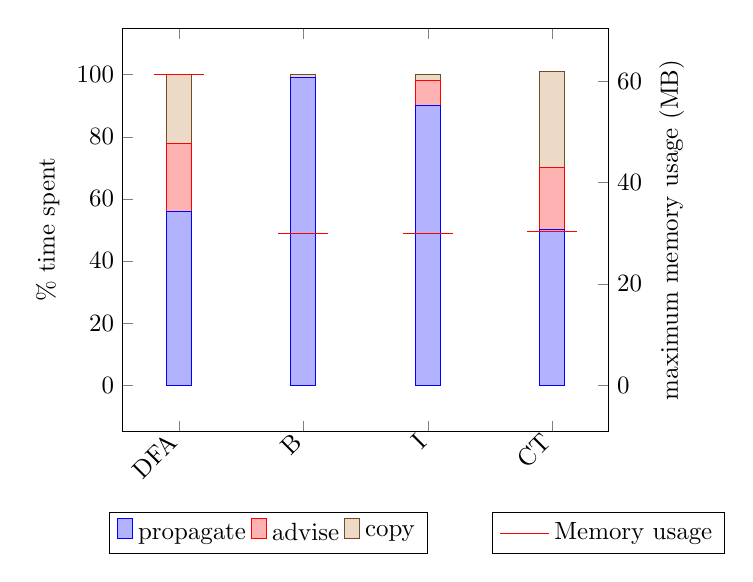
\begin{tikzpicture}[scale=0.9]
  \begin{axis}[
    ybar stacked,
    axis y line*=left,
    ymin=0,
    ymax=100,
    enlargelimits=0.15,
    legend style={at={(0.3,-0.20)},
      anchor=north,legend columns=-1},
    ylabel={\% time spent},
    symbolic x coords={DFA,B,I,CT},
    xtick=data,
    x tick label style={rotate=45,anchor=east},
    ]

    \addplot+[ybar]
      plot coordinates {
        (DFA, 56)
          (B, 99)
          (I, 90)
          (CT, 50)
          
          }; \label{ propagate }
    \addplot+[ybar]
      plot coordinates {
        (DFA, 22)
          (B, 0)
          (I, 8)
          (CT, 20)
          
          }; \label{ advise }
    \addplot+[ybar]
      plot coordinates {
        (DFA, 22)
          (B, 1)
          (I, 2)
          (CT, 31)
          
          }; \label{ copy }
    
      \legend{  }
      
      \addlegendimage{/pgfplots/refstyle=propagate}\addlegendentry{ propagate }
        
        
        \addlegendimage{/pgfplots/refstyle=advise}\addlegendentry{ advise }
        
        
        \addlegendimage{/pgfplots/refstyle=copy}\addlegendentry{ copy }
        
        
        

   \end{axis}

   \begin{axis}[
      axis y line*=right,
      axis x line=none,
      ymin=0,
      enlargelimits=0.15,
      ylabel=maximum memory usage (MB),
      legend style={at={(1.0,-0.20)},
        anchor=north,legend columns=-1},
      symbolic x coords={DFA,B,I,CT}
    ]
    \addplot+[only marks,mark size=10pt,mark=-,,mark options={.!75!red},red]
    plot coordinates {
      (DFA, 61.30859375)
      (B, 30.0390625)
      (I, 30.0390625)
      (CT, 30.29296875)
      
    };
    \addlegendentry{Memory usage}
  \end{axis}

\end{tikzpicture}

%    \vspace{\baselineskip}
  \end{minipage}\qquad
  \caption{\textbf{ Crosswords wordsVg }}
\end{figure}
\begin{figure}[t]
  \begin{minipage}[b][10cm][s]{0.45\textwidth}
    \centering
    \vfill
    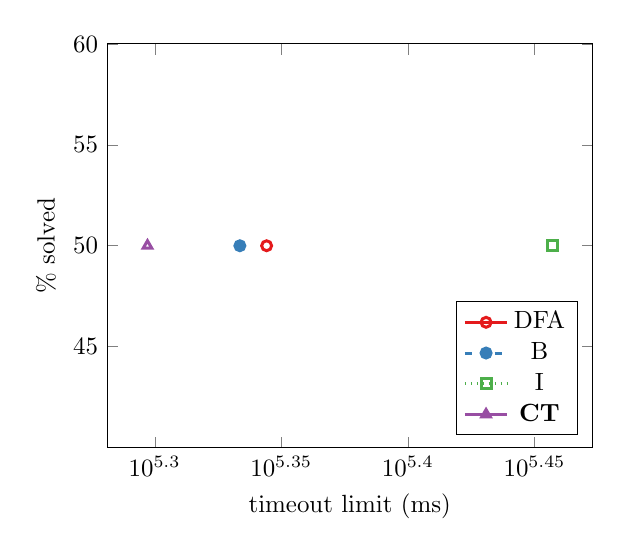
\begin{tikzpicture}[scale=0.9]
      \begin{axis}[
    xmode=log,
    every axis plot/.style={thin},
    xlabel={timeout limit (ms)},
    ylabel={\% solved},
    legend pos=south east,
    cycle list/Set1-6,
            % define fill color for the marker
            mark list fill={.!75!white},
            mark options={solid},
            cycle multiindex* list={
                Set1-6
                    \nextlist
                [3 of]linestyles
                    \nextlist
                very thick
                \nextlist
                mark=o,
                mark=*,
                mark=square,
                mark=triangle,
                mark=+
            },
    ]

    \addplot
    coordinates {
      (221050, 50)
      
    };
    \addplot
    coordinates {
      (215740, 50)
      
    };
    \addplot
    coordinates {
      (286600, 50)
      
    };
    \addplot
    coordinates {
      (198370, 50)
      
    };
    

    \legend{ DFA, B, I, \textbf{CT} }
  \end{axis}

    \end{tikzpicture}
    \vspace{\baselineskip}
  \end{minipage}\qquad
  \begin{minipage}[b][10cm][s]{0.45\textwidth}
    \centering
    \vfill
    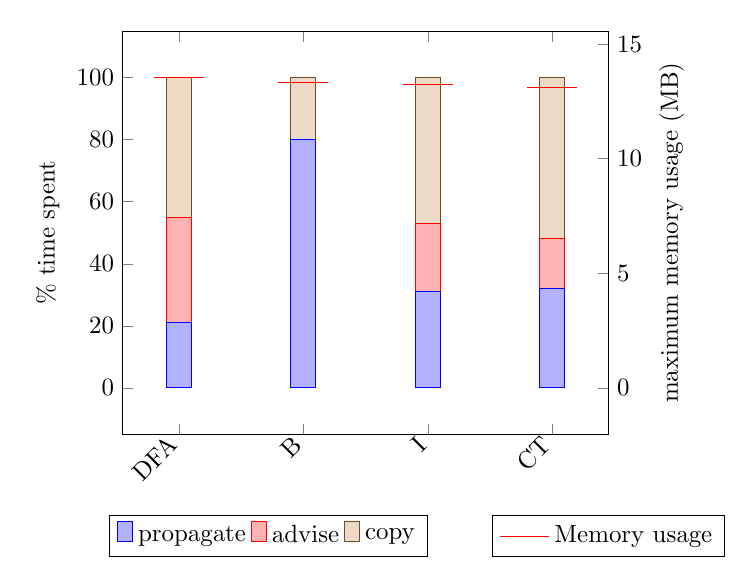
\begin{tikzpicture}[scale=0.9]
  \begin{axis}[
    ybar stacked,
    axis y line*=left,
    ymin=0,
    ymax=100,
    enlargelimits=0.15,
    legend style={at={(0.3,-0.20)},
      anchor=north,legend columns=-1},
    ylabel={\% time spent},
    symbolic x coords={DFA,B,I,CT},
    xtick=data,
    x tick label style={rotate=45,anchor=east},
    ]

    \addplot+[ybar]
      plot coordinates {
        (DFA, 21)
          (B, 80)
          (I, 31)
          (CT, 32)
          
          }; \label{ propagate }
    \addplot+[ybar]
      plot coordinates {
        (DFA, 34)
          (B, 0)
          (I, 22)
          (CT, 16)
          
          }; \label{ advise }
    \addplot+[ybar]
      plot coordinates {
        (DFA, 45)
          (B, 20)
          (I, 47)
          (CT, 52)
          
          }; \label{ copy }
    
      \legend{  }
      
      \addlegendimage{/pgfplots/refstyle=propagate}\addlegendentry{ propagate }
        
        
        \addlegendimage{/pgfplots/refstyle=advise}\addlegendentry{ advise }
        
        
        \addlegendimage{/pgfplots/refstyle=copy}\addlegendentry{ copy }
        
        
        

   \end{axis}

   \begin{axis}[
      axis y line*=right,
      axis x line=none,
      ymin=0,
      enlargelimits=0.15,
      ylabel=maximum memory usage (MB),
      legend style={at={(1.0,-0.20)},
        anchor=north,legend columns=-1},
      symbolic x coords={DFA,B,I,CT}
    ]
    \addplot+[only marks,mark size=10pt,mark=-,,mark options={.!75!red},red]
    plot coordinates {
      (DFA, 13.53515625)
      (B, 13.310546875)
      (I, 13.2421875)
      (CT, 13.115234375)
      
    };
    \addlegendentry{Memory usage}
  \end{axis}

\end{tikzpicture}

%    \vspace{\baselineskip}
  \end{minipage}\qquad
  \caption{\textbf{ Dubois }}
\end{figure}
\begin{figure}[t]
  \begin{minipage}[b][10cm][s]{0.45\textwidth}
    \centering
    \vfill
    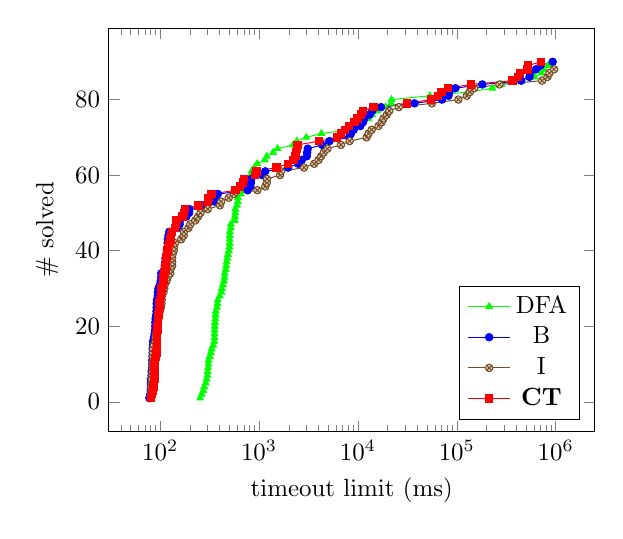
\begin{tikzpicture}[scale=0.9]
      \begin{axis}[
    xmode=log,
    every axis plot/.style={thin},
    xlabel={timeout limit (ms)},
    ylabel={\# solved},
    legend pos=south east
    % table/create on use/cumulative distribution/.style={
    %   create col/expr={\pgfmathaccuma + \thisrow{f(x)}}   
    % }
    ]
    \addplot 
    [mark=triangle*,
    mark size=1.5,
    mark options={solid},
    green] 
    coordinates {
(253.940, 1)
(262.899, 2)
(272.809, 3)
(278.671, 4)
(288.456, 5)
(294.738, 6)
(300.533, 7)
(301.856, 8)
(305.317, 9)
(307.585, 10)
(307.747, 11)
(317.045, 12)
(325.386, 13)
(331.714, 14)
(343.719, 15)
(352.611, 16)
(354.157, 17)
(354.187, 18)
(355.194, 19)
(355.670, 20)
(358.353, 21)
(361.624, 22)
(363.056, 23)
(364.990, 24)
(375.254, 25)
(379.066, 26)
(381.267, 27)
(400.323, 28)
(416.524, 29)
(419.193, 30)
(431.537, 31)
(441.410, 32)
(446.582, 33)
(449.777, 34)
(459.308, 35)
(465.151, 36)
(469.990, 37)
(476.800, 38)
(483.769, 39)
(495.431, 40)
(499.645, 41)
(504.063, 42)
(504.308, 43)
(504.525, 44)
(505.961, 45)
(518.392, 46)
(518.507, 47)
(566.413, 48)
(568.752, 49)
(575.921, 50)
(576.168, 51)
(596.357, 52)
(608.960, 53)
(610.697, 54)
(655.605, 55)
(657.724, 56)
(659.099, 57)
(661.565, 58)
(793.731, 59)
(829.897, 60)
(838.681, 61)
(897.103, 62)
(955.465, 63)
(1140.095, 64)
(1197.349, 65)
(1386.206, 66)
(1532.332, 67)
(2202.746, 68)
(2405.914, 69)
(2998.076, 70)
(4263.504, 71)
(7966.854, 72)
(8986.821, 73)
(10565.606, 74)
(12775.906, 75)
(13934.651, 76)
(15637.959, 77)
(18950.571, 78)
(21686.565, 79)
(21854.085, 80)
(53338.868, 81)
(128675.786, 82)
(229123.808, 83)
(281459.430, 84)
(391898.437, 85)
(610230.975, 86)
(714999.649, 87)
(762531.311, 88)
(838054.743, 89)
    };

    \addplot 
    [blue,
    mark=*,
    mark size=1.5,
    mark options={solid}]
    coordinates {
(77.750, 1)
(79.361, 2)
(80.110, 3)
(80.478, 4)
(80.514, 5)
(80.733, 6)
(81.819, 7)
(81.865, 8)
(82.700, 9)
(83.055, 10)
(83.084, 11)
(83.660, 12)
(83.815, 13)
(83.884, 14)
(84.339, 15)
(84.779, 16)
(86.333, 17)
(87.672, 18)
(88.800, 19)
(89.170, 20)
(89.209, 21)
(89.917, 22)
(91.234, 23)
(91.710, 24)
(92.131, 25)
(92.191, 26)
(92.825, 27)
(94.385, 28)
(94.984, 29)
(95.858, 30)
(99.363, 31)
(101.208, 32)
(102.326, 33)
(102.457, 34)
(109.924, 35)
(111.293, 36)
(112.684, 37)
(113.090, 38)
(115.314, 39)
(117.192, 40)
(118.738, 41)
(118.994, 42)
(119.411, 43)
(121.235, 44)
(123.390, 45)
(150.523, 46)
(157.344, 47)
(158.315, 48)
(182.842, 49)
(196.164, 50)
(197.579, 51)
(277.635, 52)
(354.634, 53)
(359.251, 54)
(383.268, 55)
(766.566, 56)
(816.221, 57)
(827.832, 58)
(833.240, 59)
(1081.574, 60)
(1153.362, 61)
(1963.070, 62)
(2492.142, 63)
(2701.259, 64)
(3034.945, 65)
(3062.028, 66)
(3107.310, 67)
(4356.706, 68)
(5152.815, 69)
(8143.306, 70)
(8488.009, 71)
(9065.789, 72)
(10578.592, 73)
(11242.491, 74)
(11618.200, 75)
(13121.563, 76)
(13946.231, 77)
(17115.205, 78)
(37255.008, 79)
(70596.495, 80)
(82332.599, 81)
(83994.429, 82)
(96686.082, 83)
(180912.619, 84)
(447647.179, 85)
(543188.377, 86)
(549287.562, 87)
(631674.574, 88)
(702660.342, 89)
(931931.366, 90)
    };

    \addplot [brown!60!black,
    mark options={fill=brown!40},
    mark=otimes*,
    mark size=1.5]
    coordinates {
(80.607, 1)
(80.621, 2)
(81.289, 3)
(81.598, 4)
(81.969, 5)
(82.414, 6)
(83.447, 7)
(83.492, 8)
(83.796, 9)
(83.946, 10)
(84.672, 11)
(84.778, 12)
(84.834, 13)
(85.069, 14)
(86.207, 15)
(89.293, 16)
(89.663, 17)
(90.436, 18)
(92.701, 19)
(93.412, 20)
(95.453, 21)
(96.026, 22)
(97.734, 23)
(99.208, 24)
(101.597, 25)
(103.239, 26)
(103.380, 27)
(103.698, 28)
(107.856, 29)
(109.858, 30)
(111.092, 31)
(116.012, 32)
(119.197, 33)
(126.351, 34)
(126.923, 35)
(131.997, 36)
(132.037, 37)
(132.076, 38)
(133.087, 39)
(137.356, 40)
(137.793, 41)
(141.326, 42)
(162.716, 43)
(172.556, 44)
(173.424, 45)
(192.918, 46)
(201.428, 47)
(226.385, 48)
(241.352, 49)
(255.602, 50)
(302.351, 51)
(401.666, 52)
(413.952, 53)
(493.052, 54)
(555.383, 55)
(961.003, 56)
(1155.835, 57)
(1196.833, 58)
(1202.095, 59)
(1628.244, 60)
(1659.941, 61)
(2850.318, 62)
(3611.710, 63)
(3991.524, 64)
(4242.800, 65)
(4511.471, 66)
(4915.881, 67)
(6733.256, 68)
(8232.380, 69)
(12233.495, 70)
(12792.050, 71)
(13747.597, 72)
(16126.327, 73)
(17376.344, 74)
(18154.073, 75)
(19607.670, 76)
(20742.169, 77)
(25931.910, 78)
(55946.249, 79)
(103693.950, 80)
(126173.635, 81)
(135526.885, 82)
(149917.691, 83)
(270068.501, 84)
(727604.821, 85)
(825691.112, 86)
(863292.217, 87)
(964034.894, 88)
    };

    \addplot 
    [red,
    mark size=1.5,
    mark=square*]
    coordinates {
(80.539, 1)
(82.933, 2)
(84.502, 3)
(85.194, 4)
(86.750, 5)
(87.225, 6)
(87.348, 7)
(87.379, 8)
(87.590, 9)
(87.799, 10)
(89.072, 11)
(90.371, 12)
(91.497, 13)
(92.339, 14)
(92.677, 15)
(92.786, 16)
(92.837, 17)
(93.306, 18)
(94.022, 19)
(94.387, 20)
(94.732, 21)
(94.876, 22)
(95.771, 23)
(97.088, 24)
(97.931, 25)
(98.786, 26)
(99.264, 27)
(101.340, 28)
(102.067, 29)
(102.698, 30)
(106.996, 31)
(108.150, 32)
(108.319, 33)
(109.028, 34)
(112.687, 35)
(112.838, 36)
(113.987, 37)
(115.735, 38)
(116.607, 39)
(117.896, 40)
(120.281, 41)
(124.525, 42)
(127.605, 43)
(129.317, 44)
(131.451, 45)
(140.940, 46)
(144.202, 47)
(145.438, 48)
(168.774, 49)
(174.703, 50)
(178.916, 51)
(244.908, 52)
(305.799, 53)
(306.522, 54)
(329.051, 55)
(577.969, 56)
(639.964, 57)
(687.996, 58)
(705.323, 59)
(904.996, 60)
(941.051, 61)
(1495.517, 62)
(1970.419, 63)
(2227.812, 64)
(2340.143, 65)
(2350.643, 66)
(2430.290, 67)
(2443.247, 68)
(4040.442, 69)
(6139.544, 70)
(6717.200, 71)
(7384.930, 72)
(8139.677, 73)
(9195.984, 74)
(9860.741, 75)
(10763.986, 76)
(11275.949, 77)
(14355.361, 78)
(31179.882, 79)
(55057.738, 80)
(64542.114, 81)
(70093.034, 82)
(81511.901, 83)
(138808.782, 84)
(367231.073, 85)
(417571.146, 86)
(437364.064, 87)
(519365.523, 88)
(525638.664, 89)
(705868.408, 90)
    };
    \legend{DFA,B,I,\textbf{CT}}
  \end{axis}

    \end{tikzpicture}
    \vspace{\baselineskip}
  \end{minipage}\qquad
  \begin{minipage}[b][10cm][s]{0.45\textwidth}
    \centering
    \vfill
    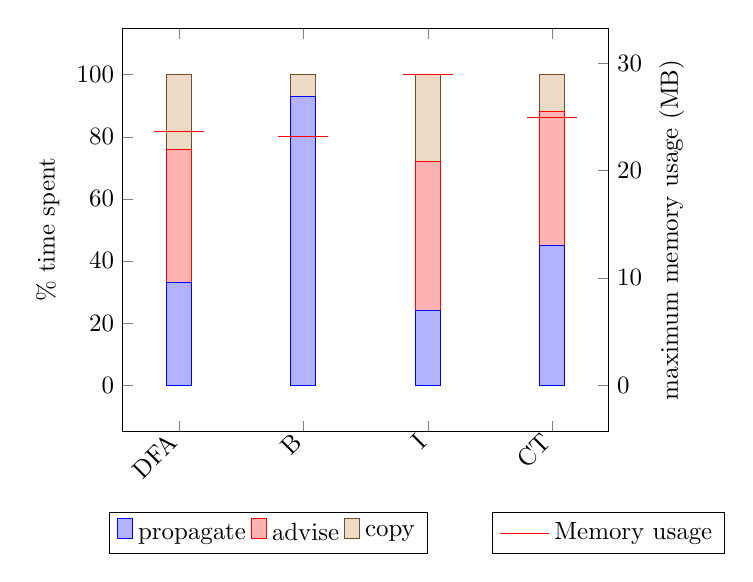
\begin{tikzpicture}[scale=0.9]
  \begin{axis}[
    ybar stacked,
    axis y line*=left,
    ymin=0,
    ymax=100,
    enlargelimits=0.15,
    legend style={at={(0.3,-0.20)},
      anchor=north,legend columns=-1},
    ylabel={\% time spent},
    symbolic x coords={DFA,B,I,CT},
    xtick=data,
    x tick label style={rotate=45,anchor=east},
    ]

    \addplot+[ybar]
      plot coordinates {
        (DFA, 33)
          (B, 93)
          (I, 24)
          (CT, 45)
          
          }; \label{ propagate }
    \addplot+[ybar]
      plot coordinates {
        (DFA, 43)
          (B, 0)
          (I, 48)
          (CT, 43)
          
          }; \label{ advise }
    \addplot+[ybar]
      plot coordinates {
        (DFA, 24)
          (B, 7)
          (I, 28)
          (CT, 12)
          
          }; \label{ copy }
    
      \legend{  }
      
      \addlegendimage{/pgfplots/refstyle=propagate}\addlegendentry{ propagate }
        
        
        \addlegendimage{/pgfplots/refstyle=advise}\addlegendentry{ advise }
        
        
        \addlegendimage{/pgfplots/refstyle=copy}\addlegendentry{ copy }
        
        
        

   \end{axis}

   \begin{axis}[
      axis y line*=right,
      axis x line=none,
      ymin=0,
      enlargelimits=0.15,
      ylabel=maximum memory usage (MB),
      legend style={at={(1.0,-0.20)},
        anchor=north,legend columns=-1},
      symbolic x coords={DFA,B,I,CT}
    ]
    \addplot+[only marks,mark size=10pt,mark=-,,mark options={.!75!red},red]
    plot coordinates {
      (DFA, 23.61328125)
      (B, 23.193359375)
      (I, 28.92578125)
      (CT, 24.921875)
      
    };
    \addlegendentry{Memory usage}
  \end{axis}

\end{tikzpicture}

%    \vspace{\baselineskip}
  \end{minipage}\qquad
  \caption{\textbf{ Geom }}
\end{figure}
\begin{figure}[t]
  \begin{minipage}[b][10cm][s]{0.45\textwidth}
    \centering
    \vfill
    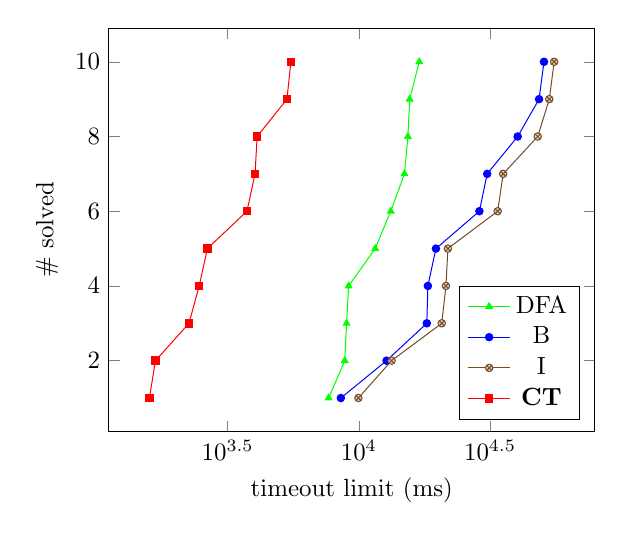
\begin{tikzpicture}[scale=0.9]
      \begin{axis}[
    xmode=log,
    every axis plot/.style={thin},
    xlabel={timeout limit (ms)},
    ylabel={\# solved},
    legend pos=south east
    % table/create on use/cumulative distribution/.style={
    %   create col/expr={\pgfmathaccuma + \thisrow{f(x)}}   
    % }
    ]
    \addplot 
    [mark=triangle*,
    mark size=1.5,
    mark options={solid},
    green] 
    coordinates {
    (7669.883, 1)
(8836.338, 2)
(8977.330, 3)
(9140.777, 4)
(11537.562, 5)
(13231.384, 6)
(14923.762, 7)
(15381.136, 8)
(15623.402, 9)
(16994.255, 10)
    };

    \addplot 
    [blue,
    mark=*,
    mark size=1.5,
    mark options={solid}]
    coordinates {
    (8538.228, 1)
(12749.685, 2)
(18156.956, 3)
(18327.323, 4)
(19669.292, 5)
(28802.590, 6)
(30835.715, 7)
(40301.654, 8)
(48620.995, 9)
(50774.009, 10)
    };

    \addplot [brown!60!black,
    mark options={fill=brown!40},
    mark=otimes*,
    mark size=1.5]
    coordinates {
    (9960.047, 1)
(13326.927, 2)
(20700.530, 3)
(21474.840, 4)
(21842.271, 5)
(33817.893, 6)
(35489.987, 7)
(48049.593, 8)
(53196.297, 9)
(55499.785, 10)
    };

    \addplot 
    [red,
    mark size=1.5,
    mark=square*]
    coordinates {
    (1591.239, 1)
(1678.457, 2)
(2251.773, 3)
(2462.919, 4)
(2646.514, 5)
(3745.993, 6)
(4020.526, 7)
(4095.836, 8)
(5320.617, 9)
(5507.353, 10)
    };
    \legend{DFA,B,I,\textbf{CT}}
  \end{axis}

    \end{tikzpicture}
    \vspace{\baselineskip}
  \end{minipage}\qquad
  \begin{minipage}[b][10cm][s]{0.45\textwidth}
    \centering
    \vfill
    \input{ tba.tex }
%    \vspace{\baselineskip}
  \end{minipage}\qquad
  \caption{\textbf{ K5 }}
\end{figure}
\begin{figure}[t]
  \begin{minipage}[b][10cm][s]{0.45\textwidth}
    \centering
    \vfill
    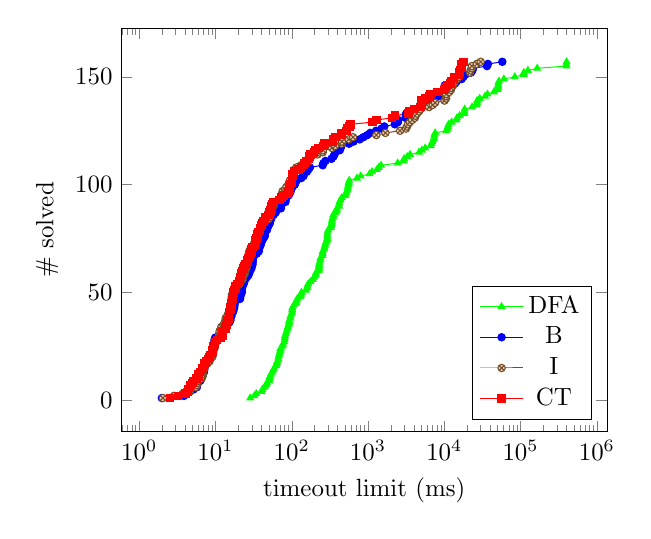
\begin{tikzpicture}[scale=0.9]
      \begin{axis}[
    xmode=log,
    every axis plot/.style={thin},
    xlabel={timeout limit (ms)},
    ylabel={\# solved},
    legend pos=south east
    % table/create on use/cumulative distribution/.style={
    %   create col/expr={\pgfmathaccuma + \thisrow{f(x)}}   
    % }
    ]
    \addplot 
    [mark=triangle*,
    mark size=1.5,
    mark options={solid},
    green] 
    coordinates {
    (28.479, 1)
(32.259, 2)
(34.184, 3)
(40.176, 4)
(41.117, 5)
(44.220, 6)
(46.524, 7)
(47.119, 8)
(50.594, 9)
(51.185, 10)
(51.683, 11)
(53.094, 12)
(55.381, 13)
(57.551, 14)
(58.822, 15)
(62.806, 16)
(64.164, 17)
(64.612, 18)
(66.816, 19)
(66.879, 20)
(68.064, 21)
(69.387, 22)
(70.958, 23)
(71.154, 24)
(74.896, 25)
(76.696, 26)
(79.628, 27)
(80.614, 28)
(80.994, 29)
(81.915, 30)
(83.799, 31)
(85.498, 32)
(87.376, 33)
(88.955, 34)
(90.775, 35)
(92.387, 36)
(92.399, 37)
(95.672, 38)
(96.038, 39)
(99.560, 40)
(101.063, 41)
(101.351, 42)
(102.343, 43)
(105.757, 44)
(114.544, 45)
(115.689, 46)
(117.793, 47)
(129.374, 48)
(131.156, 49)
(134.382, 50)
(152.723, 51)
(159.993, 52)
(160.432, 53)
(164.374, 54)
(176.218, 55)
(188.673, 56)
(197.819, 57)
(205.739, 58)
(207.344, 59)
(226.014, 60)
(227.529, 61)
(227.659, 62)
(227.801, 63)
(232.632, 64)
(236.122, 65)
(237.853, 66)
(253.358, 67)
(253.590, 68)
(254.330, 69)
(266.274, 70)
(268.730, 71)
(273.463, 72)
(277.735, 73)
(288.026, 74)
(291.548, 75)
(292.756, 76)
(293.227, 77)
(294.410, 78)
(300.709, 79)
(327.569, 80)
(332.541, 81)
(333.924, 82)
(334.411, 83)
(339.586, 84)
(348.199, 85)
(349.532, 86)
(371.373, 87)
(386.701, 88)
(390.963, 89)
(418.408, 90)
(418.695, 91)
(422.230, 92)
(437.503, 93)
(453.861, 94)
(502.971, 95)
(520.108, 96)
(527.304, 97)
(542.192, 98)
(544.013, 99)
(554.465, 100)
(558.086, 101)
(567.256, 102)
(715.556, 103)
(800.577, 104)
(1046.040, 105)
(1129.254, 106)
(1306.675, 107)
(1383.006, 108)
(1479.749, 109)
(2448.671, 110)
(2930.847, 111)
(2965.572, 112)
(3260.970, 113)
(3556.870, 114)
(4656.549, 115)
(5078.367, 116)
(5623.653, 117)
(6659.340, 118)
(6784.312, 119)
(6973.103, 120)
(7329.557, 121)
(7359.121, 122)
(7396.106, 123)
(7576.040, 124)
(10610.895, 125)
(10922.259, 126)
(11159.351, 127)
(11396.117, 128)
(12483.028, 129)
(14419.922, 130)
(14676.118, 131)
(15906.106, 132)
(18283.308, 133)
(18442.544, 134)
(18470.312, 135)
(23102.428, 136)
(26464.714, 137)
(26805.377, 138)
(26954.579, 139)
(29112.162, 140)
(34228.839, 141)
(36846.271, 142)
(44695.427, 143)
(50105.717, 144)
(50810.695, 145)
(50811.889, 146)
(51055.360, 147)
(51994.297, 148)
(60294.547, 149)
(83881.093, 150)
(110031.542, 151)
(110303.654, 152)
(124680.954, 153)
(164840.449, 154)
(398572.615, 155)
(398573.318, 156)
(401037.607, 157)
    };

    \addplot 
    [blue,
    mark=*,
    mark size=1.5,
    mark options={solid}]
    coordinates {
    (1.981, 1)
(3.865, 2)
(4.064, 3)
(4.147, 4)
(5.164, 5)
(5.702, 6)
(5.759, 7)
(5.839, 8)
(6.320, 9)
(6.503, 10)
(6.645, 11)
(6.804, 12)
(7.058, 13)
(7.115, 14)
(7.149, 15)
(7.349, 16)
(7.424, 17)
(7.744, 18)
(8.081, 19)
(8.255, 20)
(9.006, 21)
(9.029, 22)
(9.159, 23)
(9.557, 24)
(9.613, 25)
(9.675, 26)
(9.691, 27)
(9.705, 28)
(9.922, 29)
(11.049, 30)
(11.959, 31)
(12.363, 32)
(13.100, 33)
(13.492, 34)
(14.116, 35)
(15.142, 36)
(15.661, 37)
(15.767, 38)
(16.210, 39)
(16.247, 40)
(17.023, 41)
(17.310, 42)
(17.589, 43)
(17.712, 44)
(17.876, 45)
(18.383, 46)
(20.996, 47)
(21.124, 48)
(21.524, 49)
(22.126, 50)
(22.138, 51)
(22.244, 52)
(22.755, 53)
(23.472, 54)
(23.827, 55)
(24.361, 56)
(25.737, 57)
(27.024, 58)
(27.729, 59)
(28.322, 60)
(29.453, 61)
(30.020, 62)
(30.589, 63)
(30.689, 64)
(30.830, 65)
(31.200, 66)
(31.809, 67)
(34.778, 68)
(36.914, 69)
(36.958, 70)
(38.037, 71)
(39.151, 72)
(39.381, 73)
(40.922, 74)
(42.232, 75)
(44.223, 76)
(44.334, 77)
(44.614, 78)
(47.327, 79)
(47.856, 80)
(49.569, 81)
(51.504, 82)
(51.951, 83)
(53.451, 84)
(54.347, 85)
(57.828, 86)
(61.396, 87)
(63.159, 88)
(72.148, 89)
(72.466, 90)
(72.988, 91)
(82.727, 92)
(83.052, 93)
(85.267, 94)
(91.016, 95)
(94.242, 96)
(97.150, 97)
(97.576, 98)
(102.403, 99)
(109.460, 100)
(112.204, 101)
(115.663, 102)
(132.942, 103)
(142.599, 104)
(142.756, 105)
(158.121, 106)
(164.564, 107)
(173.027, 108)
(254.761, 109)
(260.341, 110)
(276.465, 111)
(331.631, 112)
(352.139, 113)
(362.559, 114)
(375.144, 115)
(427.109, 116)
(436.286, 117)
(447.651, 118)
(565.156, 119)
(646.826, 120)
(776.447, 121)
(868.556, 122)
(978.473, 123)
(1068.681, 124)
(1274.319, 125)
(1503.918, 126)
(1634.250, 127)
(2243.783, 128)
(2467.649, 129)
(2483.835, 130)
(3099.528, 131)
(3157.027, 132)
(3161.783, 133)
(3741.648, 134)
(3951.777, 135)
(5102.101, 136)
(5232.868, 137)
(5786.206, 138)
(6318.847, 139)
(7243.252, 140)
(8487.686, 141)
(9904.149, 142)
(10127.961, 143)
(10128.039, 144)
(10128.112, 145)
(10128.150, 146)
(13891.478, 147)
(14623.462, 148)
(16877.665, 149)
(17802.422, 150)
(18785.664, 151)
(22435.458, 152)
(23340.568, 153)
(23707.641, 154)
(36289.195, 155)
(37329.808, 156)
(57612.194, 157)
    };

    \addplot [brown!60!black,
    mark options={fill=brown!40},
    mark=otimes*,
    mark size=1.5]
    coordinates {
    (2.040, 1)
(2.855, 2)
(3.719, 3)
(4.632, 4)
(4.641, 5)
(5.533, 6)
(5.714, 7)
(5.787, 8)
(5.857, 9)
(6.577, 10)
(6.773, 11)
(6.786, 12)
(6.845, 13)
(7.010, 14)
(7.176, 15)
(7.222, 16)
(7.831, 17)
(8.350, 18)
(8.396, 19)
(9.065, 20)
(9.266, 21)
(9.307, 22)
(9.310, 23)
(9.701, 24)
(9.813, 25)
(9.942, 26)
(9.968, 27)
(10.442, 28)
(10.956, 29)
(11.109, 30)
(11.272, 31)
(11.322, 32)
(11.721, 33)
(11.918, 34)
(12.829, 35)
(13.226, 36)
(13.534, 37)
(13.610, 38)
(14.211, 39)
(14.646, 40)
(15.410, 41)
(15.583, 42)
(15.762, 43)
(15.958, 44)
(15.963, 45)
(16.254, 46)
(16.279, 47)
(16.369, 48)
(16.443, 49)
(17.092, 50)
(17.486, 51)
(18.263, 52)
(19.356, 53)
(20.741, 54)
(21.061, 55)
(22.659, 56)
(22.736, 57)
(23.631, 58)
(24.292, 59)
(24.320, 60)
(25.417, 61)
(25.501, 62)
(25.852, 63)
(26.675, 64)
(26.775, 65)
(26.937, 66)
(27.206, 67)
(27.302, 68)
(27.716, 69)
(28.500, 70)
(30.188, 71)
(31.872, 72)
(32.316, 73)
(33.242, 74)
(35.322, 75)
(35.465, 76)
(35.935, 77)
(36.585, 78)
(37.473, 79)
(39.837, 80)
(41.395, 81)
(41.916, 82)
(43.633, 83)
(49.626, 84)
(51.364, 85)
(51.918, 86)
(54.007, 87)
(54.632, 88)
(54.830, 89)
(57.738, 90)
(57.962, 91)
(59.061, 92)
(66.911, 93)
(72.484, 94)
(73.188, 95)
(75.152, 96)
(76.043, 97)
(82.614, 98)
(85.390, 99)
(92.294, 100)
(92.310, 101)
(94.799, 102)
(100.399, 103)
(103.386, 104)
(104.357, 105)
(107.466, 106)
(108.809, 107)
(115.076, 108)
(132.377, 109)
(150.485, 110)
(155.998, 111)
(165.401, 112)
(168.692, 113)
(217.693, 114)
(254.736, 115)
(256.005, 116)
(335.905, 117)
(372.441, 118)
(450.372, 119)
(454.066, 120)
(558.160, 121)
(636.164, 122)
(1284.240, 123)
(1689.710, 124)
(2626.867, 125)
(3141.959, 126)
(3250.413, 127)
(3340.003, 128)
(3529.547, 129)
(3796.970, 130)
(4107.852, 131)
(4203.355, 132)
(4401.731, 133)
(4666.155, 134)
(4868.455, 135)
(6318.847, 136)
(7041.570, 137)
(7569.985, 138)
(10060.819, 139)
(10560.355, 140)
(10560.410, 141)
(10579.580, 142)
(11617.533, 143)
(12234.257, 144)
(12293.138, 145)
(13063.427, 146)
(13446.632, 147)
(13581.502, 148)
(14784.440, 149)
(15562.642, 150)
(15729.409, 151)
(21672.499, 152)
(22165.904, 153)
(22926.964, 154)
(22968.641, 155)
(26660.677, 156)
(30020.990, 157)
    };

    \addplot 
    [red,
    mark size=1.5,
    mark=square*]
    coordinates {
    (2.524, 1)
(3.206, 2)
(4.039, 3)
(4.361, 4)
(4.389, 5)
(4.606, 6)
(4.710, 7)
(4.978, 8)
(5.167, 9)
(5.663, 10)
(5.980, 11)
(6.008, 12)
(6.225, 13)
(6.704, 14)
(6.753, 15)
(7.063, 16)
(7.226, 17)
(7.490, 18)
(7.986, 19)
(8.325, 20)
(8.460, 21)
(9.034, 22)
(9.147, 23)
(9.285, 24)
(9.408, 25)
(9.836, 26)
(9.925, 27)
(10.386, 28)
(11.817, 29)
(12.283, 30)
(12.371, 31)
(12.421, 32)
(13.446, 33)
(13.626, 34)
(13.946, 35)
(14.115, 36)
(14.294, 37)
(14.926, 38)
(14.986, 39)
(15.113, 40)
(15.153, 41)
(15.708, 42)
(15.817, 43)
(16.104, 44)
(16.300, 45)
(16.366, 46)
(16.700, 47)
(17.004, 48)
(17.051, 49)
(17.135, 50)
(17.819, 51)
(18.200, 52)
(18.311, 53)
(19.536, 54)
(20.424, 55)
(20.802, 56)
(21.035, 57)
(21.612, 58)
(22.023, 59)
(22.282, 60)
(23.361, 61)
(23.547, 62)
(24.895, 63)
(26.247, 64)
(26.330, 65)
(27.079, 66)
(28.241, 67)
(28.749, 68)
(29.706, 69)
(29.737, 70)
(30.669, 71)
(32.885, 72)
(33.265, 73)
(33.377, 74)
(34.736, 75)
(35.312, 76)
(35.602, 77)
(36.702, 78)
(38.075, 79)
(38.642, 80)
(39.762, 81)
(40.766, 82)
(42.725, 83)
(44.467, 84)
(45.569, 85)
(49.392, 86)
(50.013, 87)
(52.813, 88)
(53.668, 89)
(54.022, 90)
(54.956, 91)
(56.929, 92)
(69.097, 93)
(73.566, 94)
(77.968, 95)
(88.625, 96)
(90.543, 97)
(92.817, 98)
(93.189, 99)
(95.409, 100)
(100.775, 101)
(100.882, 102)
(101.361, 103)
(101.829, 104)
(101.889, 105)
(106.477, 106)
(122.410, 107)
(131.500, 108)
(145.337, 109)
(147.842, 110)
(155.328, 111)
(167.560, 112)
(171.786, 113)
(175.499, 114)
(197.262, 115)
(200.902, 116)
(225.599, 117)
(258.897, 118)
(267.365, 119)
(347.569, 120)
(348.248, 121)
(372.442, 122)
(443.611, 123)
(448.073, 124)
(523.765, 125)
(529.761, 126)
(572.104, 127)
(590.425, 128)
(1147.457, 129)
(1293.023, 130)
(2054.343, 131)
(2255.645, 132)
(3386.939, 133)
(3464.006, 134)
(4036.434, 135)
(4860.082, 136)
(4930.466, 137)
(4994.702, 138)
(5017.154, 139)
(5624.775, 140)
(6438.068, 141)
(6595.553, 142)
(8133.711, 143)
(9914.384, 144)
(10152.289, 145)
(10890.155, 146)
(11982.889, 147)
(12241.757, 148)
(13446.630, 149)
(13446.658, 150)
(15582.920, 151)
(15915.676, 152)
(15960.351, 153)
(16824.803, 154)
(16825.085, 155)
(16895.618, 156)
(17839.722, 157)
    };
    \legend{DFA,B,I,CT}
  \end{axis}

    \end{tikzpicture}
    \vspace{\baselineskip}
  \end{minipage}\qquad
  \begin{minipage}[b][10cm][s]{0.45\textwidth}
    \centering
    \vfill
    \input{ tba.tex }
%    \vspace{\baselineskip}
  \end{minipage}\qquad
  \caption{\textbf{ Kakuro Easy }}
\end{figure}
\begin{figure}[t]
  \begin{minipage}[b][10cm][s]{0.45\textwidth}
    \centering
    \vfill
    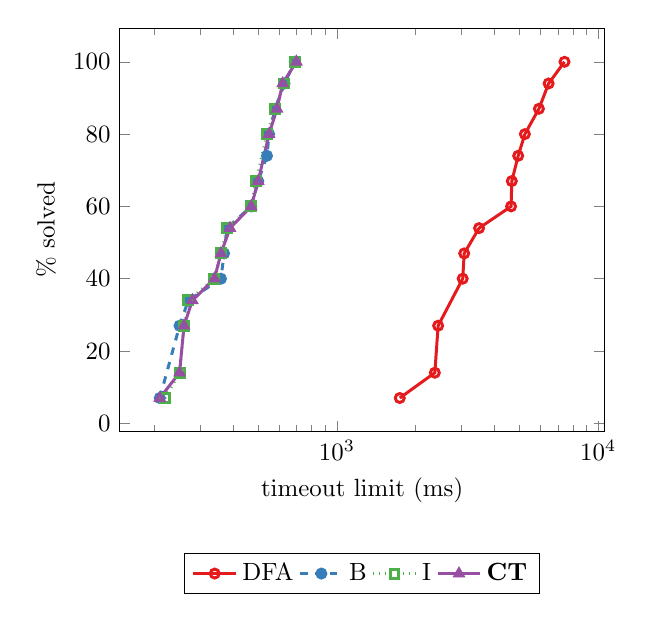
\begin{tikzpicture}[scale=0.9]
      \begin{axis}[
    xmode=log,
    every axis plot/.style={thin},
    xlabel={timeout limit (ms)},
    ylabel={\% solved},
    legend style={at={(0.5,-0.30)},
      anchor=north,legend columns=-1},
    % legend pos=south east,
    cycle list/Set1-6,
            % define fill color for the marker
            mark list fill={.!75!white},
            mark options={solid,scale=0.9},
            cycle multiindex* list={
                Set1-6
                    \nextlist
                [3 of]linestyles
                    \nextlist
                very thick
                \nextlist
                mark=o,
                mark=*,
                mark=square,
                mark=triangle,
                mark=+
            },
    ]

    \addplot
    coordinates {
      (1740, 7)
      (2370, 14)
      (2440, 27)
      (3030, 40)
      (3070, 47)
      (3500, 54)
      (4640, 60)
      (4670, 67)
      (4940, 74)
      (5240, 80)
      (5930, 87)
      (6460, 94)
      (7430, 100)
      
    };
    \addplot
    coordinates {
      (210, 7)
      (250, 27)
      (270, 34)
      (360, 40)
      (370, 47)
      (380, 54)
      (470, 60)
      (500, 67)
      (540, 74)
      (550, 80)
      (580, 87)
      (630, 94)
      (690, 100)
      
    };
    \addplot
    coordinates {
      (220, 7)
      (250, 14)
      (260, 27)
      (270, 34)
      (340, 40)
      (360, 47)
      (380, 54)
      (470, 60)
      (490, 67)
      (540, 80)
      (580, 87)
      (630, 94)
      (690, 100)
      
    };
    \addplot
    coordinates {
      (210, 7)
      (250, 14)
      (260, 27)
      (280, 34)
      (340, 40)
      (360, 47)
      (390, 54)
      (470, 60)
      (500, 67)
      (550, 80)
      (590, 87)
      (620, 94)
      (700, 100)
      
    };
    

    \legend{ DFA, B, I, \textbf{CT} }
  \end{axis}

    \end{tikzpicture}
    \vspace{\baselineskip}
  \end{minipage}\qquad
  \begin{minipage}[b][10cm][s]{0.45\textwidth}
    \centering
    \vfill
    \input{ tba.tex }
%    \vspace{\baselineskip}
  \end{minipage}\qquad
  \caption{\textbf{ Kakuro Medium }}
\end{figure}
\begin{figure}[t]
  \begin{minipage}[b][10cm][s]{0.45\textwidth}
    \centering
    \vfill
    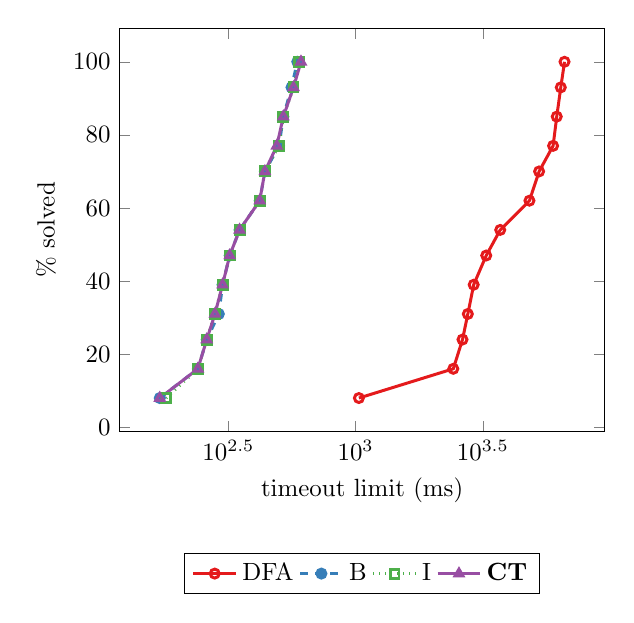
\begin{tikzpicture}[scale=0.9]
      \begin{axis}[
    xmode=log,
    every axis plot/.style={thin},
    xlabel={timeout limit (ms)},
    ylabel={\% solved},
    legend style={at={(0.5,-0.30)},
      anchor=north,legend columns=-1},
    % legend pos=south east,
    cycle list/Set1-6,
            % define fill color for the marker
            mark list fill={.!75!white},
            mark options={solid,scale=0.9},
            cycle multiindex* list={
                Set1-6
                    \nextlist
                [3 of]linestyles
                    \nextlist
                very thick
                \nextlist
                mark=o,
                mark=*,
                mark=square,
                mark=triangle,
                mark=+
            },
    ]

    \addplot
    coordinates {
      (1030, 8)
      (2420, 16)
      (2630, 24)
      (2760, 31)
      (2910, 39)
      (3260, 47)
      (3700, 54)
      (4820, 62)
      (5260, 70)
      (5970, 77)
      (6170, 85)
      (6400, 93)
      (6620, 100)
      
    };
    \addplot
    coordinates {
      (170, 8)
      (240, 16)
      (260, 24)
      (290, 31)
      (300, 39)
      (320, 47)
      (350, 54)
      (420, 62)
      (440, 70)
      (500, 77)
      (520, 85)
      (560, 93)
      (590, 100)
      
    };
    \addplot
    coordinates {
      (180, 8)
      (240, 16)
      (260, 24)
      (280, 31)
      (300, 39)
      (320, 47)
      (350, 54)
      (420, 62)
      (440, 70)
      (500, 77)
      (520, 85)
      (570, 93)
      (600, 100)
      
    };
    \addplot
    coordinates {
      (170, 8)
      (240, 16)
      (260, 24)
      (280, 31)
      (300, 39)
      (320, 47)
      (350, 54)
      (420, 62)
      (440, 70)
      (490, 77)
      (520, 85)
      (570, 93)
      (610, 100)
      
    };
    

    \legend{ DFA, B, I, \textbf{CT} }
  \end{axis}

    \end{tikzpicture}
    \vspace{\baselineskip}
  \end{minipage}\qquad
  \begin{minipage}[b][10cm][s]{0.45\textwidth}
    \centering
    \vfill
    \input{ tba.tex }
%    \vspace{\baselineskip}
  \end{minipage}\qquad
  \caption{\textbf{ Kakuro Hard }}
\end{figure}
\begin{figure}[t]
  \begin{minipage}[b][10cm][s]{0.45\textwidth}
    \centering
    \vfill
    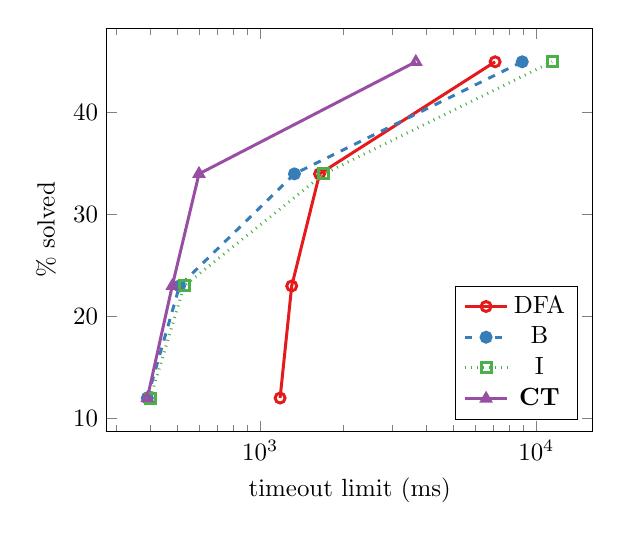
\begin{tikzpicture}[scale=0.9]
      \begin{axis}[
    xmode=log,
    every axis plot/.style={thin},
    xlabel={timeout limit (ms)},
    ylabel={\% solved},
    legend pos=south east,
    cycle list/Set1-6,
            % define fill color for the marker
            mark list fill={.!75!white},
            mark options={solid},
            cycle multiindex* list={
                Set1-6
                    \nextlist
                [3 of]linestyles
                    \nextlist
                very thick
                \nextlist
                mark=o,
                mark=*,
                mark=square,
                mark=triangle,
                mark=+
            },
    ]

    \addplot
    coordinates {
      (1180, 12)
      (1300, 23)
      (1640, 34)
      (7090, 45)
      
    };
    \addplot
    coordinates {
      (390, 12)
      (510, 23)
      (1330, 34)
      (8890, 45)
      
    };
    \addplot
    coordinates {
      (400, 12)
      (530, 23)
      (1700, 34)
      (11400, 45)
      
    };
    \addplot
    coordinates {
      (390, 12)
      (480, 23)
      (600, 34)
      (3660, 45)
      
    };
    

    \legend{ DFA, B, I, \textbf{CT} }
  \end{axis}

    \end{tikzpicture}
    \vspace{\baselineskip}
  \end{minipage}\qquad
  \begin{minipage}[b][10cm][s]{0.45\textwidth}
    \centering
    \vfill
    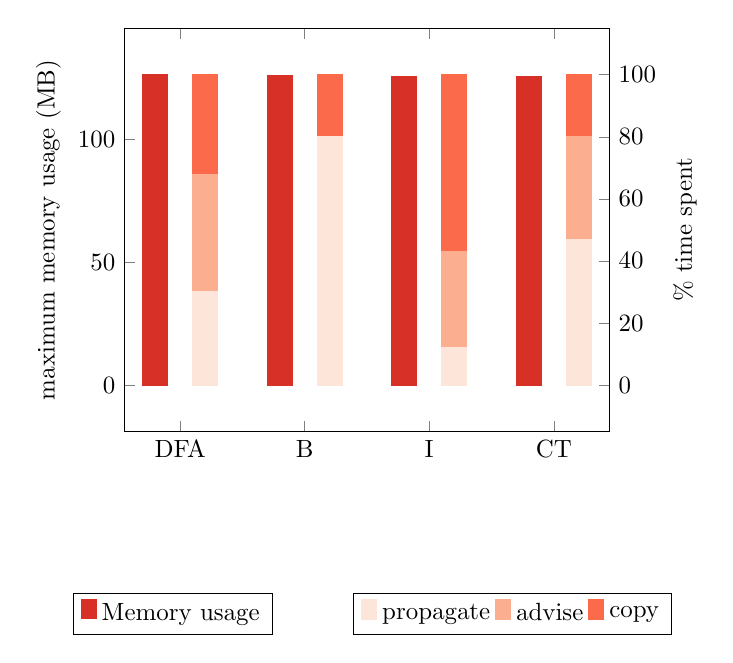
\begin{tikzpicture}[scale=0.9]
  
  \begin{axis}[
    ybar stacked,
    every axis plot/.append style={fill},
    axis y line*=left,
    ymin=0,
    enlargelimits=0.15,
    ylabel=maximum memory usage (MB),
    legend style={at={(0.1,-0.40)},
      anchor=north,legend columns=-1},
    symbolic x coords={DFA,B,I,CT},
    cycle list name=RdYlGn-9
    ]
    \addplot+[ybar,bar width=10pt,mark=none,xshift=-10pt]
    plot coordinates {
      (DFA, 126.279296875)
      (B, 125.76171875)
      (I, 125.634765625)
      (CT, 125.458984375)
      
    };
    \addlegendentry{Memory usage}
  \end{axis}

  \begin{axis}[
    ybar stacked,
    every axis plot/.append style={fill},
    axis x line=none,
    axis y line*=right,
    ymin=0,
    ymax=100,
    enlargelimits=0.15,
    legend style={at={(0.8,-0.40)},
      anchor=north,legend columns=-1},
    ylabel={\% time spent},
    symbolic x coords={DFA,B,I,CT},
    xtick=data,
    cycle list name=Reds-4,
    x tick label style={rotate=45,anchor=east},
    ]

    \addplot+[ybar,xshift=10pt]
      plot coordinates {
        (DFA, 30)
          (B, 80)
          (I, 12)
          (CT, 47)
          
          }; \label{ propagate }
    \addplot+[ybar,xshift=10pt]
      plot coordinates {
        (DFA, 38)
          (B, 0)
          (I, 31)
          (CT, 33)
          
          }; \label{ advise }
    \addplot+[ybar,xshift=10pt]
      plot coordinates {
        (DFA, 32)
          (B, 20)
          (I, 57)
          (CT, 20)
          
          }; \label{ copy }
    
      \legend{  }
      
      \addlegendimage{/pgfplots/refstyle=propagate}\addlegendentry{ propagate }
        
        \addlegendimage{/pgfplots/refstyle=advise}\addlegendentry{ advise }
        
        \addlegendimage{/pgfplots/refstyle=copy}\addlegendentry{ copy }
        
        

   \end{axis}

\end{tikzpicture}

%    \vspace{\baselineskip}
  \end{minipage}\qquad
  \caption{\textbf{ Langford 2 }}
\end{figure}
\begin{figure}[t]
  \begin{minipage}[b][10cm][s]{0.45\textwidth}
    \centering
    \vfill
    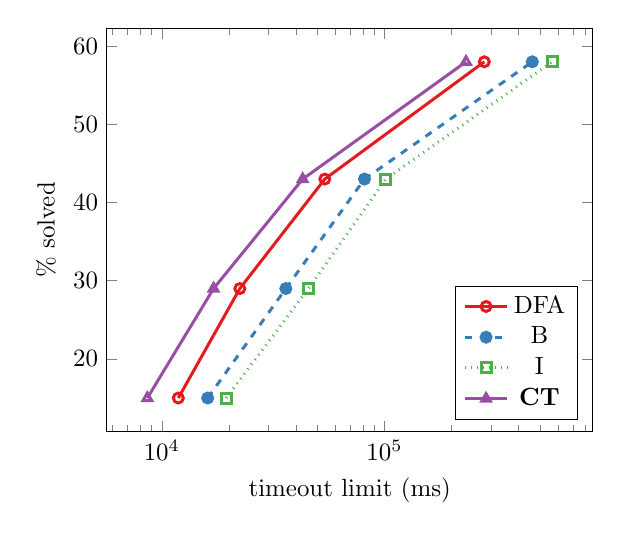
\begin{tikzpicture}[scale=0.9]
      \begin{axis}[
    xmode=log,
    every axis plot/.style={thin},
    xlabel={timeout limit (ms)},
    ylabel={\% solved},
    legend pos=south east,
    cycle list/Set1-6,
            % define fill color for the marker
            mark list fill={.!75!white},
            mark options={solid},
            cycle multiindex* list={
                Set1-6
                    \nextlist
                [3 of]linestyles
                    \nextlist
                very thick
                \nextlist
                mark=o,
                mark=*,
                mark=square,
                mark=triangle,
                mark=+
            },
    ]

    \addplot
    coordinates {
      (11860, 15)
      (22400, 29)
      (53920, 43)
      (280500, 58)
      
    };
    \addplot
    coordinates {
      (16070, 15)
      (36050, 29)
      (81280, 43)
      (460580, 58)
      
    };
    \addplot
    coordinates {
      (19450, 15)
      (45590, 29)
      (101350, 43)
      (565200, 58)
      
    };
    \addplot
    coordinates {
      (8610, 15)
      (17080, 29)
      (42900, 43)
      (232160, 58)
      
    };
    

    \legend{ DFA, B, I, \textbf{CT} }
  \end{axis}

    \end{tikzpicture}
    \vspace{\baselineskip}
  \end{minipage}\qquad
  \begin{minipage}[b][10cm][s]{0.45\textwidth}
    \centering
    \vfill
    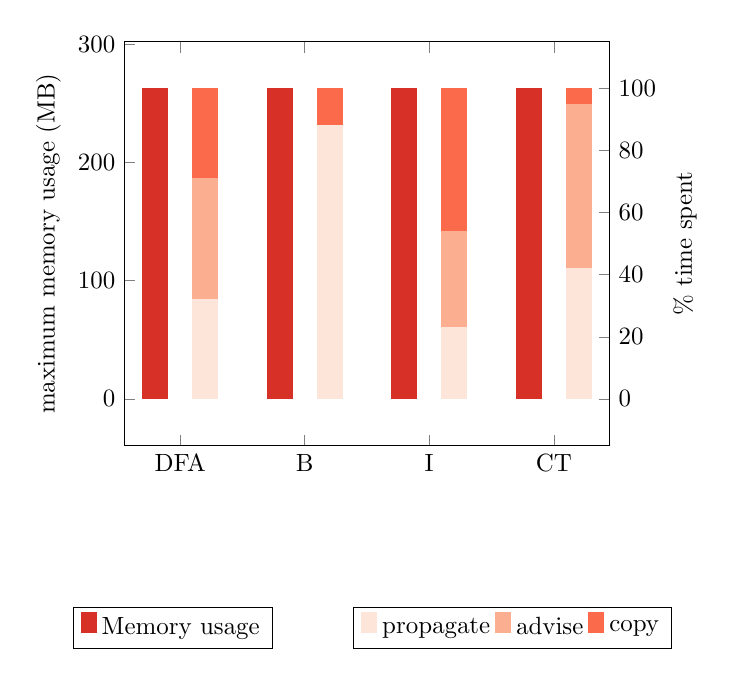
\begin{tikzpicture}[scale=0.9]
  
  \begin{axis}[
    ybar stacked,
    every axis plot/.append style={fill},
    axis y line*=left,
    ymin=0,
    enlargelimits=0.15,
    ylabel=maximum memory usage (MB),
    legend style={at={(0.1,-0.40)},
      anchor=north,legend columns=-1},
    symbolic x coords={DFA,B,I,CT},
    cycle list name=RdYlGn-9
    ]
    \addplot+[ybar,bar width=10pt,mark=none,xshift=-10pt]
    plot coordinates {
      (DFA, 262.36328125)
      (B, 262.265625)
      (I, 262.158203125)
      (CT, 262.03125)
      
    };
    \addlegendentry{Memory usage}
  \end{axis}

  \begin{axis}[
    ybar stacked,
    every axis plot/.append style={fill},
    axis x line=none,
    axis y line*=right,
    ymin=0,
    ymax=100,
    enlargelimits=0.15,
    legend style={at={(0.8,-0.40)},
      anchor=north,legend columns=-1},
    ylabel={\% time spent},
    symbolic x coords={DFA,B,I,CT},
    xtick=data,
    cycle list name=Reds-4,
    x tick label style={rotate=45,anchor=east},
    ]

    \addplot+[ybar,xshift=10pt]
      plot coordinates {
        (DFA, 32)
          (B, 88)
          (I, 23)
          (CT, 42)
          
          }; \label{ propagate }
    \addplot+[ybar,xshift=10pt]
      plot coordinates {
        (DFA, 39)
          (B, 0)
          (I, 31)
          (CT, 53)
          
          }; \label{ advise }
    \addplot+[ybar,xshift=10pt]
      plot coordinates {
        (DFA, 29)
          (B, 12)
          (I, 46)
          (CT, 5)
          
          }; \label{ copy }
    
      \legend{  }
      
      \addlegendimage{/pgfplots/refstyle=propagate}\addlegendentry{ propagate }
        
        \addlegendimage{/pgfplots/refstyle=advise}\addlegendentry{ advise }
        
        \addlegendimage{/pgfplots/refstyle=copy}\addlegendentry{ copy }
        
        

   \end{axis}

\end{tikzpicture}

%    \vspace{\baselineskip}
  \end{minipage}\qquad
  \caption{\textbf{ Langford 3 }}
\end{figure}
\begin{figure}[t]
  \begin{minipage}[b][10cm][s]{0.45\textwidth}
    \centering
    \vfill
    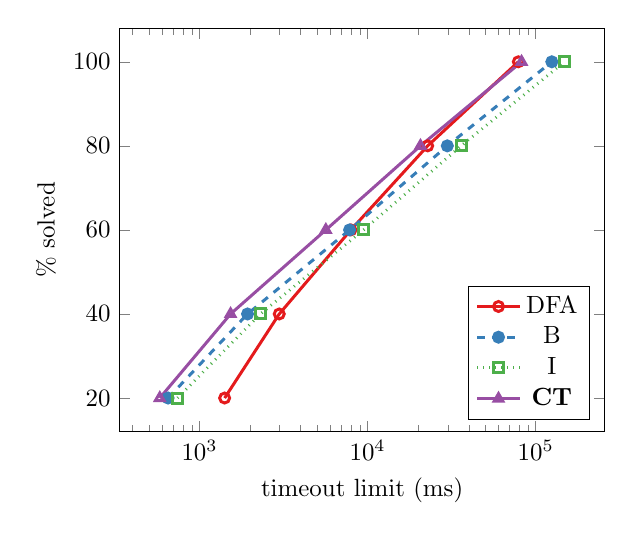
\begin{tikzpicture}[scale=0.9]
      \begin{axis}[
    xmode=log,
    every axis plot/.style={thin},
    xlabel={timeout limit (ms)},
    ylabel={\% solved},
    legend pos=south east,
    cycle list/Set1-6,
            % define fill color for the marker
            mark list fill={.!75!white},
            mark options={solid},
            cycle multiindex* list={
                Set1-6
                    \nextlist
                [3 of]linestyles
                    \nextlist
                very thick
                \nextlist
                mark=o,
                mark=*,
                mark=square,
                mark=triangle,
                mark=+
            },
    ]

    \addplot
    coordinates {
      (1410, 20)
      (2980, 40)
      (7950, 60)
      (22760, 80)
      (78820, 100)
      
    };
    \addplot
    coordinates {
      (650, 20)
      (1930, 40)
      (7810, 60)
      (29790, 80)
      (124670, 100)
      
    };
    \addplot
    coordinates {
      (740, 20)
      (2300, 40)
      (9460, 60)
      (36010, 80)
      (148310, 100)
      
    };
    \addplot
    coordinates {
      (580, 20)
      (1530, 40)
      (5640, 60)
      (20620, 80)
      (82360, 100)
      
    };
    

    \legend{ DFA, B, I, \textbf{CT} }
  \end{axis}

    \end{tikzpicture}
    \vspace{\baselineskip}
  \end{minipage}\qquad
  \begin{minipage}[b][10cm][s]{0.45\textwidth}
    \centering
    \vfill
    \input{ tba.tex }
%    \vspace{\baselineskip}
  \end{minipage}\qquad
  \caption{\textbf{ Langford 4 }}
\end{figure}
\begin{figure}[t]
  \begin{minipage}[b][10cm][s]{0.45\textwidth}
    \centering
    \vfill
    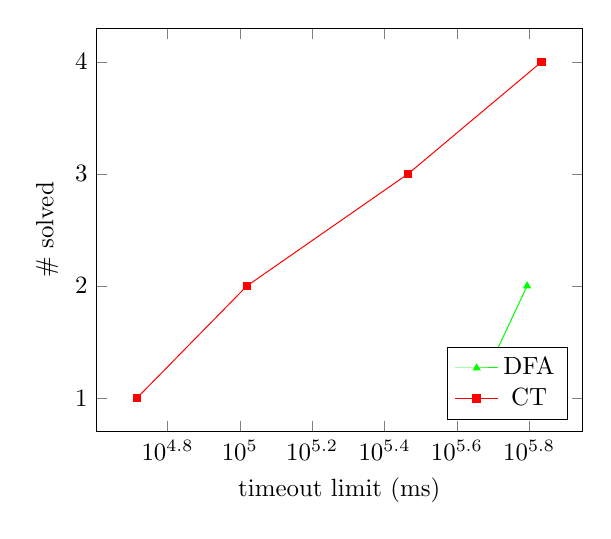
\begin{tikzpicture}[scale=0.9]
      \begin{axis}[
    xmode=log,
    every axis plot/.style={thin},
    xlabel={timeout limit (ms)},
    ylabel={\# solved},
    legend pos=south east
    % table/create on use/cumulative distribution/.style={
    %   create col/expr={\pgfmathaccuma + \thisrow{f(x)}}   
    % }
    ]
    \addplot 
    [mark=triangle*,
    mark size=1.5,
    mark options={solid},
    green] 
    coordinates {
    (445273.296, 1)
(622414.790, 2)
% (1031281.648, 3)
% (1073752.509, 4)
% (1077338.303, 5)
% (1078117.880, 6)
% (1078636.961, 7)
% (1079178.894, 8)
% (1079839.216, 9)
% (1080840.349, 10)
% (1082059.397, 11)
% (1083648.155, 12)
% (1083902.339, 13)
% (1083988.269, 14)
% (1084069.534, 15)
% (1084396.676, 16)
% (1085666.524, 17)
% (1089495.967, 18)
% (1091132.921, 19)
% (1091433.340, 20)
% (1092057.252, 21)
% (1093916.092, 22)
% (1094177.223, 23)
% (1114453.122, 24)
% (1115067.373, 25)
    };

%     \addplot 
%     [blue,
%     mark=*,
%     mark size=1.5,
%     mark options={solid}]
%     coordinates {
%     (1004672.786, 1)
% (1004695.224, 2)
% (1004696.645, 3)
% (1004718.463, 4)
% (1004738.023, 5)
% (1004743.967, 6)
% (1004751.151, 7)
% (1004765.567, 8)
% (1004781.515, 9)
% (1004797.803, 10)
% (1004816.640, 11)
% (1004820.096, 12)
% (1004835.673, 13)
% (1004864.792, 14)
% (1004881.537, 15)
% (1004913.526, 16)
% (1004920.059, 17)
% (1004929.625, 18)
% (1004958.448, 19)
% (1004996.508, 20)
% (1005007.752, 21)
% (1005029.139, 22)
% (1005067.535, 23)
% (1005104.606, 24)
% (1040982.750, 25)
%     };

%     \addplot [brown!60!black,
%     mark options={fill=brown!40},
%     mark=otimes*,
%     mark size=1.5]
%     coordinates {
%     (1004653.569, 1)
% (1004695.464, 2)
% (1004715.665, 3)
% (1004725.629, 4)
% (1004729.598, 5)
% (1004736.757, 6)
% (1004768.906, 7)
% (1004774.513, 8)
% (1004800.095, 9)
% (1004877.671, 10)
% (1004885.444, 11)
% (1004924.289, 12)
% (1004954.273, 13)
% (1004976.220, 14)
% (1005012.748, 15)
% (1005016.479, 16)
% (1005025.501, 17)
% (1005059.309, 18)
% (1005081.774, 19)
% (1005131.686, 20)
% (1005177.022, 21)
% (1005199.107, 22)
% (1005247.884, 23)
% (1005272.462, 24)
% (1103825.908, 25)
%     };

    \addplot 
    [red,
    mark size=1.5,
    mark=square*]
    coordinates {
    (51933.780, 1)
(104573.439, 2)
(291800.057, 3)
(683133.039, 4)
% (1006259.610, 5)
% (1006270.822, 6)
% (1006282.419, 7)
% (1006303.104, 8)
% (1006319.339, 9)
% (1006423.422, 10)
% (1006449.607, 11)
% (1006459.928, 12)
% (1006499.500, 13)
% (1006510.783, 14)
% (1006510.952, 15)
% (1006511.373, 16)
% (1006567.036, 17)
% (1006579.356, 18)
% (1006588.135, 19)
% (1006591.883, 20)
% (1006659.196, 21)
% (1006817.280, 22)
% (1006986.645, 23)
% (1012355.582, 24)
% (1025624.781, 25)
    };
    \legend{DFA,CT}
  \end{axis}

    \end{tikzpicture}
    \vspace{\baselineskip}
  \end{minipage}\qquad
  \begin{minipage}[b][10cm][s]{0.45\textwidth}
    \centering
    \vfill
    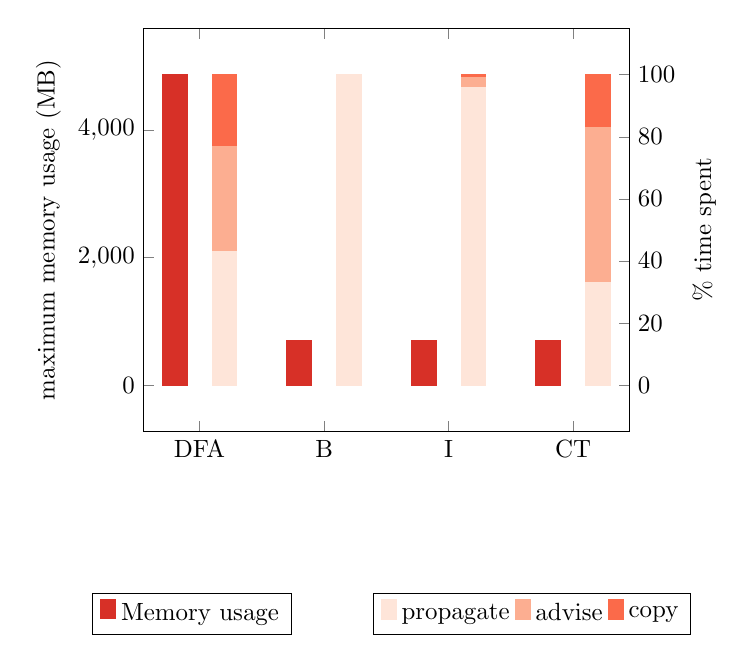
\begin{tikzpicture}[scale=0.9]
  
  \begin{axis}[
    ybar stacked,
    every axis plot/.append style={fill},
    axis y line*=left,
    ymin=0,
    enlargelimits=0.15,
    ylabel=maximum memory usage (MB),
    legend style={at={(0.1,-0.40)},
      anchor=north,legend columns=-1},
    symbolic x coords={DFA,B,I,CT},
    cycle list name=RdYlGn-9
    ]
    \addplot+[ybar,bar width=10pt,mark=none,xshift=-10pt]
    plot coordinates {
      (DFA, 4864.921875)
      (B, 705.224609375)
      (I, 703.9453125)
      (CT, 704.62890625)
      
    };
    \addlegendentry{Memory usage}
  \end{axis}

  \begin{axis}[
    ybar stacked,
    every axis plot/.append style={fill},
    axis x line=none,
    axis y line*=right,
    ymin=0,
    ymax=100,
    enlargelimits=0.15,
    legend style={at={(0.8,-0.40)},
      anchor=north,legend columns=-1},
    ylabel={\% time spent},
    symbolic x coords={DFA,B,I,CT},
    xtick=data,
    cycle list name=Reds-4,
    x tick label style={rotate=45,anchor=east},
    ]

    \addplot+[ybar,xshift=10pt]
      plot coordinates {
        (DFA, 43)
          (B, 100)
          (I, 96)
          (CT, 33)
          
          }; \label{ propagate }
    \addplot+[ybar,xshift=10pt]
      plot coordinates {
        (DFA, 34)
          (B, 0)
          (I, 3)
          (CT, 50)
          
          }; \label{ advise }
    \addplot+[ybar,xshift=10pt]
      plot coordinates {
        (DFA, 23)
          (B, 0)
          (I, 1)
          (CT, 17)
          
          }; \label{ copy }
    
      \legend{  }
      
      \addlegendimage{/pgfplots/refstyle=propagate}\addlegendentry{ propagate }
        
        \addlegendimage{/pgfplots/refstyle=advise}\addlegendentry{ advise }
        
        \addlegendimage{/pgfplots/refstyle=copy}\addlegendentry{ copy }
        
        

   \end{axis}

\end{tikzpicture}

%    \vspace{\baselineskip}
  \end{minipage}\qquad
  \caption{\textbf{ MDD 05 }}
\end{figure}
\begin{figure}[t]
  \begin{minipage}[b][10cm][s]{0.45\textwidth}
    \centering
    \vfill
    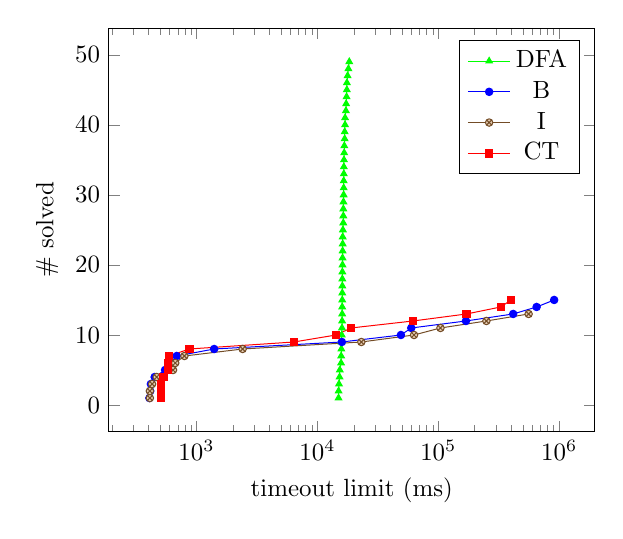
\begin{tikzpicture}[scale=0.9]
      \begin{axis}[
    xmode=log,
    every axis plot/.style={thin},
    xlabel={timeout limit (ms)},
    ylabel={\# solved},
    legend pos=north east
    % table/create on use/cumulative distribution/.style={
    %   create col/expr={\pgfmathaccuma + \thisrow{f(x)}}   
    % }
    ]
    \addplot 
    [mark=triangle*,
    mark size=1.5,
    mark options={solid},
    green] 
    coordinates {
    (14955.640, 1)
(14968.715, 2)
(15081.852, 3)
(15246.230, 4)
(15319.517, 5)
(15694.443, 6)
(15719.960, 7)
(15775.606, 8)
(15786.850, 9)
(15896.231, 10)
(15965.343, 11)
(16005.555, 12)
(16025.117, 13)
(16031.876, 14)
(16045.846, 15)
(16051.370, 16)
(16069.886, 17)
(16072.811, 18)
(16083.237, 19)
(16121.665, 20)
(16136.113, 21)
(16156.801, 22)
(16176.375, 23)
(16178.653, 24)
(16245.676, 25)
(16366.799, 26)
(16378.158, 27)
(16380.892, 28)
(16416.757, 29)
(16478.895, 30)
(16497.038, 31)
(16500.046, 32)
(16533.794, 33)
(16540.436, 34)
(16585.806, 35)
(16652.982, 36)
(16691.128, 37)
(16800.390, 38)
(16810.154, 39)
(16925.261, 40)
(16928.061, 41)
(17203.760, 42)
(17283.698, 43)
(17423.272, 44)
(17512.601, 45)
(17538.616, 46)
(17769.707, 47)
(18045.623, 48)
(18343.375, 49)
    };

    \addplot 
    [blue,
    mark=*,
    mark size=1.5,
    mark options={solid}]
    coordinates {
    (407.759, 1)
(414.434, 2)
(419.216, 3)
(450.778, 4)
(549.394, 5)
(610.163, 6)
(686.273, 7)
(1398.874, 8)
(15928.727, 9)
(49039.533, 10)
(59721.595, 11)
(169215.924, 12)
(415997.085, 13)
(649968.448, 14)
(907521.385, 15)
% (1000382.106, 16)
% (1000387.429, 17)
% (1000388.151, 18)
% (1000388.347, 19)
% (1000390.684, 20)
% (1000395.468, 21)
% (1000398.451, 22)
% (1000400.524, 23)
% (1000400.706, 24)
% (1000401.730, 25)
% (1000401.841, 26)
% (1000403.654, 27)
% (1000403.994, 28)
% (1000404.160, 29)
% (1000404.725, 30)
% (1000405.072, 31)
% (1000406.271, 32)
% (1000406.289, 33)
% (1000408.137, 34)
% (1000409.168, 35)
% (1000409.171, 36)
% (1000409.900, 37)
% (1000409.919, 38)
% (1000410.346, 39)
% (1000411.211, 40)
% (1000412.274, 41)
% (1000412.434, 42)
% (1000413.669, 43)
% (1000413.697, 44)
% (1000413.893, 45)
% (1000415.159, 46)
% (1000415.655, 47)
% (1000416.766, 48)
% (1000417.147, 49)
    };

    \addplot [brown!60!black,
    mark options={fill=brown!40},
    mark=otimes*,
    mark size=1.5]
    coordinates {
    (411.425, 1)
(411.643, 2)
(429.292, 3)
(468.693, 4)
(639.628, 5)
(667.122, 6)
(794.022, 7)
(2406.553, 8)
(23078.974, 9)
(62957.355, 10)
(104153.981, 11)
(249841.503, 12)
(558201.118, 13)
% (1000388.044, 14)
% (1000402.477, 15)
% (1000403.436, 16)
% (1000404.783, 17)
% (1000405.378, 18)
% (1000405.704, 19)
% (1000406.897, 20)
% (1000406.968, 21)
% (1000407.434, 22)
% (1000407.466, 23)
% (1000408.430, 24)
% (1000410.331, 25)
% (1000411.890, 26)
% (1000412.483, 27)
% (1000413.619, 28)
% (1000413.815, 29)
% (1000414.349, 30)
% (1000417.491, 31)
% (1000417.949, 32)
% (1000418.050, 33)
% (1000418.110, 34)
% (1000419.106, 35)
% (1000421.213, 36)
% (1000425.194, 37)
% (1000425.968, 38)
% (1000429.409, 39)
% (1000430.069, 40)
% (1000430.274, 41)
% (1000431.550, 42)
% (1000431.958, 43)
% (1000434.278, 44)
% (1000435.376, 45)
% (1000437.954, 46)
% (1000465.864, 47)
% (1000470.438, 48)
% (1000485.931, 49)
    };

    \addplot 
    [red,
    mark size=1.5,
    mark=square*]
    coordinates {
    (508.071, 1)
(509.196, 2)
(510.855, 3)
(534.756, 4)
(578.458, 5)
(581.294, 6)
(592.155, 7)
(871.362, 8)
(6376.939, 9)
(14282.674, 10)
(18970.185, 11)
(61800.545, 12)
(171097.990, 13)
(328543.590, 14)
(399691.539, 15)
% (1000508.452, 16)
% (1000510.576, 17)
% (1000511.037, 18)
% (1000515.800, 19)
% (1000516.296, 20)
% (1000522.133, 21)
% (1000522.266, 22)
% (1000527.510, 23)
% (1000527.510, 24)
% (1000530.273, 25)
% (1000530.582, 26)
% (1000535.684, 27)
% (1000536.663, 28)
% (1000538.258, 29)
% (1000538.752, 30)
% (1000538.821, 31)
% (1000539.927, 32)
% (1000542.929, 33)
% (1000543.075, 34)
% (1000543.682, 35)
% (1000543.865, 36)
% (1000547.730, 37)
% (1000548.803, 38)
% (1000549.065, 39)
% (1000549.762, 40)
% (1000552.156, 41)
% (1000552.610, 42)
% (1000560.835, 43)
% (1000562.921, 44)
% (1000565.715, 45)
% (1000567.437, 46)
% (1000570.129, 47)
% (1000576.494, 48)
% (1000627.930, 49)
    };
    \legend{DFA,B,I,CT}
  \end{axis}

    \end{tikzpicture}
    \vspace{\baselineskip}
  \end{minipage}\qquad
  \begin{minipage}[b][10cm][s]{0.45\textwidth}
    \centering
    \vfill
    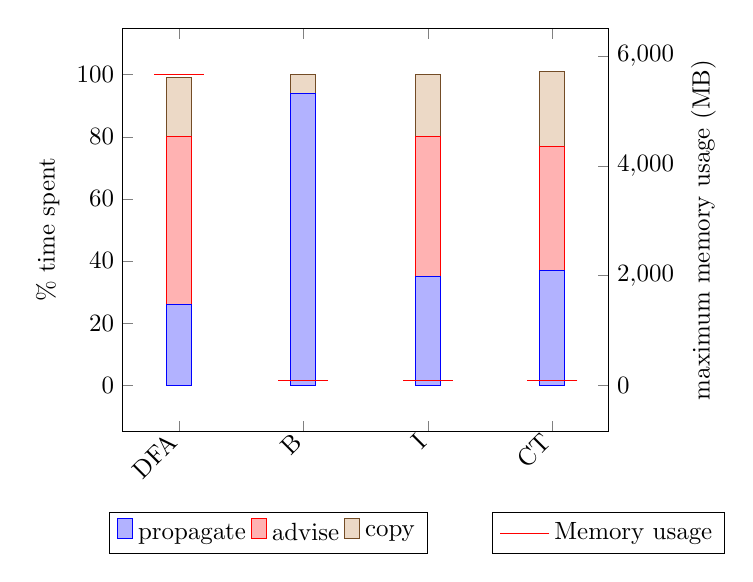
\begin{tikzpicture}[scale=0.9]
  \begin{axis}[
    ybar stacked,
    axis y line*=left,
    ymin=0,
    ymax=100,
    enlargelimits=0.15,
    legend style={at={(0.3,-0.20)},
      anchor=north,legend columns=-1},
    ylabel={\% time spent},
    symbolic x coords={DFA,B,I,CT},
    xtick=data,
    x tick label style={rotate=45,anchor=east},
    ]

    \addplot+[ybar]
      plot coordinates {
        (DFA, 26)
          (B, 94)
          (I, 35)
          (CT, 37)
          
          }; \label{ propagate }
    \addplot+[ybar]
      plot coordinates {
        (DFA, 54)
          (B, 0)
          (I, 45)
          (CT, 40)
          
          }; \label{ advise }
    \addplot+[ybar]
      plot coordinates {
        (DFA, 19)
          (B, 6)
          (I, 20)
          (CT, 24)
          
          }; \label{ copy }
    
      \legend{  }
      
      \addlegendimage{/pgfplots/refstyle=propagate}\addlegendentry{ propagate }
        
        
        \addlegendimage{/pgfplots/refstyle=advise}\addlegendentry{ advise }
        
        
        \addlegendimage{/pgfplots/refstyle=copy}\addlegendentry{ copy }
        
        
        

   \end{axis}

   \begin{axis}[
      axis y line*=right,
      axis x line=none,
      ymin=0,
      enlargelimits=0.15,
      ylabel=maximum memory usage (MB),
      legend style={at={(1.0,-0.20)},
        anchor=north,legend columns=-1},
      symbolic x coords={DFA,B,I,CT}
    ]
    \addplot+[only marks,mark size=10pt,mark=-,,mark options={.!75!red},red]
    plot coordinates {
      (DFA, 5660.048828125)
      (B, 76.962890625)
      (I, 76.62109375)
      (CT, 76.416015625)
      
    };
    \addlegendentry{Memory usage}
  \end{axis}

\end{tikzpicture}

%    \vspace{\baselineskip}
  \end{minipage}\qquad
  \caption{\textbf{ Mod Renault }}
\end{figure}
\begin{figure}[t]
  \begin{minipage}[b][10cm][s]{0.45\textwidth}
    \centering
    \vfill
    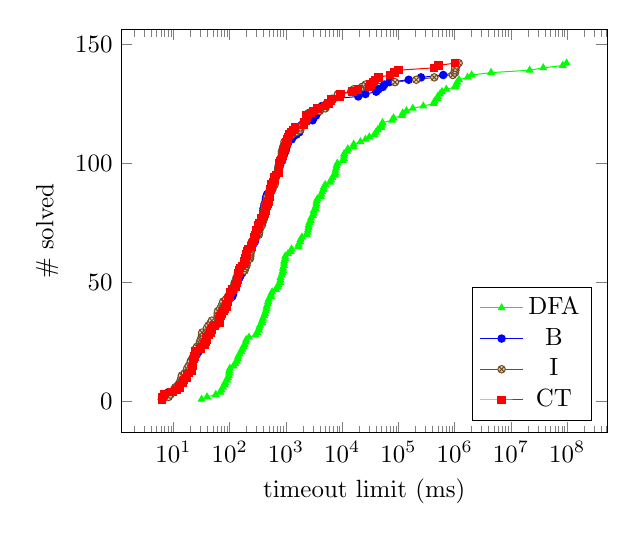
\begin{tikzpicture}[scale=0.9]
      \begin{axis}[
    xmode=log,
    every axis plot/.style={thin},
    xlabel={timeout limit (ms)},
    ylabel={\# solved},
    legend pos=south east
    % table/create on use/cumulative distribution/.style={
    %   create col/expr={\pgfmathaccuma + \thisrow{f(x)}}   
    % }
    ]
    \addplot 
    [mark=triangle*,
    mark size=1.5,
    mark options={solid},
    green] 
    coordinates {
    (31.696, 1)
(39.559, 2)
(56.508, 3)
(68.178, 4)
(70.931, 5)
(75.984, 6)
(81.689, 7)
(82.437, 8)
(90.551, 9)
(92.696, 10)
(96.318, 11)
(97.489, 12)
(98.251, 13)
(100.928, 14)
(116.739, 15)
(124.823, 16)
(132.967, 17)
(139.159, 18)
(141.636, 19)
(149.509, 20)
(161.219, 21)
(165.144, 22)
(176.745, 23)
(182.586, 24)
(193.826, 25)
(196.443, 26)
(220.596, 27)
(287.801, 28)
(307.637, 29)
(331.351, 30)
(335.110, 31)
(344.194, 32)
(377.529, 33)
(378.932, 34)
(389.655, 35)
(410.350, 36)
(423.248, 37)
(438.655, 38)
(450.859, 39)
(454.186, 40)
(475.260, 41)
(483.019, 42)
(493.122, 43)
(544.266, 44)
(544.377, 45)
(568.390, 46)
(658.959, 47)
(704.627, 48)
(733.115, 49)
(790.697, 50)
(796.819, 51)
(799.668, 52)
(839.106, 53)
(863.117, 54)
(884.469, 55)
(886.545, 56)
(921.009, 57)
(927.374, 58)
(928.500, 59)
(970.121, 60)
(970.451, 61)
(1084.311, 62)
(1214.035, 63)
(1256.732, 64)
(1667.050, 65)
(1679.067, 66)
(1790.603, 67)
(1813.082, 68)
(1923.256, 69)
(2334.693, 70)
(2424.581, 71)
(2460.778, 72)
(2524.488, 73)
(2535.289, 74)
(2608.483, 75)
(2727.527, 76)
(2790.777, 77)
(3010.831, 78)
(3089.396, 79)
(3100.186, 80)
(3342.097, 81)
(3421.319, 82)
(3476.286, 83)
(3498.766, 84)
(3603.983, 85)
(4152.208, 86)
(4252.733, 87)
(4414.005, 88)
(4619.485, 89)
(4703.303, 90)
(4995.143, 91)
(6104.482, 92)
(6327.657, 93)
(6680.221, 94)
(7451.205, 95)
(7524.283, 96)
(7577.742, 97)
(7815.366, 98)
(7963.806, 99)
(8190.616, 100)
(10239.338, 101)
(10646.387, 102)
(10743.772, 103)
(10816.354, 104)
(12183.647, 105)
(12608.953, 106)
(15986.466, 107)
(16016.047, 108)
(21085.457, 109)
(25840.612, 110)
(30330.074, 111)
(37303.992, 112)
(39784.632, 113)
(42867.757, 114)
(49654.939, 115)
(49896.816, 116)
(51937.811, 117)
(76626.715, 118)
(81762.693, 119)
(116690.715, 120)
(118979.114, 121)
(138352.575, 122)
(179596.690, 123)
(275896.959, 124)
(422494.853, 125)
(435710.733, 126)
(490650.459, 127)
(500154.998, 128)
(546044.177, 129)
(592457.334, 130)
(707795.890, 131)
(1014847.682, 132)
(1051973.108, 133)
(1109712.990, 134)
(1188811.633, 135)
(1691073.549, 136)
(1998815.209, 137)
(4412151.304, 138)
(21464315.090, 139)
(37446981.305, 140)
(83163795.720, 141)
(97236200.525, 142)
    };

    \addplot 
    [blue,
    mark=*,
    mark size=1.5,
    mark options={solid}]
    coordinates {
    (6.266, 1)
(6.620, 2)
(7.191, 3)
(8.174, 4)
(10.291, 5)
(11.099, 6)
(12.126, 7)
(13.714, 8)
(14.201, 9)
(17.122, 10)
(17.173, 11)
(18.736, 12)
(19.358, 13)
(19.989, 14)
(20.187, 15)
(20.291, 16)
(20.437, 17)
(21.788, 18)
(22.787, 19)
(26.326, 20)
(28.086, 21)
(28.501, 22)
(30.269, 23)
(30.327, 24)
(31.429, 25)
(32.957, 26)
(35.312, 27)
(37.683, 28)
(42.027, 29)
(44.010, 30)
(45.270, 31)
(57.413, 32)
(58.136, 33)
(60.287, 34)
(63.612, 35)
(64.377, 36)
(70.203, 37)
(71.636, 38)
(74.510, 39)
(81.417, 40)
(81.885, 41)
(86.850, 42)
(98.379, 43)
(110.554, 44)
(114.955, 45)
(116.342, 46)
(116.797, 47)
(117.697, 48)
(127.569, 49)
(128.638, 50)
(132.319, 51)
(149.619, 52)
(156.554, 53)
(167.748, 54)
(171.866, 55)
(177.579, 56)
(186.974, 57)
(188.731, 58)
(197.746, 59)
(206.427, 60)
(212.854, 61)
(223.093, 62)
(234.349, 63)
(237.887, 64)
(249.281, 65)
(261.335, 66)
(279.625, 67)
(282.633, 68)
(287.627, 69)
(297.860, 70)
(315.101, 71)
(322.909, 72)
(331.748, 73)
(351.193, 74)
(352.948, 75)
(363.872, 76)
(366.739, 77)
(390.571, 78)
(395.284, 79)
(397.359, 80)
(399.002, 81)
(410.756, 82)
(418.082, 83)
(436.759, 84)
(439.198, 85)
(447.297, 86)
(462.840, 87)
(504.442, 88)
(543.477, 89)
(559.175, 90)
(566.240, 91)
(601.149, 92)
(619.715, 93)
(652.612, 94)
(657.839, 95)
(715.983, 96)
(731.157, 97)
(752.783, 98)
(784.906, 99)
(794.121, 100)
(856.340, 101)
(862.438, 102)
(901.933, 103)
(927.762, 104)
(979.127, 105)
(1000.759, 106)
(1023.428, 107)
(1067.513, 108)
(1074.968, 109)
(1265.279, 110)
(1331.799, 111)
(1538.059, 112)
(1731.374, 113)
(1737.023, 114)
(1790.519, 115)
(1895.419, 116)
(2041.525, 117)
(2975.267, 118)
(3105.441, 119)
(3430.058, 120)
(3574.657, 121)
(3985.434, 122)
(4137.262, 123)
(4364.834, 124)
(5314.336, 125)
(6189.835, 126)
(6463.719, 127)
(19294.688, 128)
(25874.502, 129)
(40075.340, 130)
(44076.314, 131)
(52831.470, 132)
(56117.125, 133)
(69049.283, 134)
(151946.681, 135)
(251788.612, 136)
(624723.233, 137)
(1006224.760, 138)
(1024927.746, 139)
(1025126.900, 140)
(1051096.785, 141)
(1054709.554, 142)
    };

    \addplot [brown!60!black,
    mark options={fill=brown!40},
    mark=otimes*,
    mark size=1.5]
    coordinates {
    (6.225, 1)
(8.252, 2)
(8.866, 3)
(8.903, 4)
(10.276, 5)
(10.793, 6)
(12.246, 7)
(12.967, 8)
(13.482, 9)
(13.873, 10)
(14.125, 11)
(15.975, 12)
(17.388, 13)
(17.590, 14)
(18.641, 15)
(20.043, 16)
(20.476, 17)
(21.613, 18)
(23.615, 19)
(24.164, 20)
(24.372, 21)
(24.882, 22)
(26.053, 23)
(29.400, 24)
(29.513, 25)
(30.549, 26)
(31.898, 27)
(32.205, 28)
(32.366, 29)
(39.353, 30)
(39.524, 31)
(42.127, 32)
(45.853, 33)
(48.185, 34)
(60.297, 35)
(60.940, 36)
(61.286, 37)
(61.970, 38)
(67.684, 39)
(71.354, 40)
(74.374, 41)
(76.755, 42)
(86.492, 43)
(92.532, 44)
(102.074, 45)
(107.118, 46)
(110.458, 47)
(119.452, 48)
(120.692, 49)
(122.537, 50)
(130.211, 51)
(131.757, 52)
(139.069, 53)
(139.341, 54)
(184.184, 55)
(187.471, 56)
(198.576, 57)
(201.040, 58)
(207.945, 59)
(229.958, 60)
(232.188, 61)
(233.976, 62)
(239.163, 63)
(240.688, 64)
(241.932, 65)
(243.311, 66)
(245.547, 67)
(265.954, 68)
(292.029, 69)
(328.546, 70)
(334.072, 71)
(336.358, 72)
(350.752, 73)
(375.324, 74)
(379.234, 75)
(396.967, 76)
(401.683, 77)
(401.895, 78)
(405.570, 79)
(411.227, 80)
(417.570, 81)
(419.966, 82)
(421.977, 83)
(456.664, 84)
(458.121, 85)
(467.458, 86)
(514.809, 87)
(537.183, 88)
(573.529, 89)
(585.083, 90)
(628.983, 91)
(629.151, 92)
(638.579, 93)
(655.494, 94)
(683.596, 95)
(719.854, 96)
(720.103, 97)
(726.177, 98)
(743.018, 99)
(776.859, 100)
(788.068, 101)
(801.667, 102)
(840.869, 103)
(844.819, 104)
(845.660, 105)
(882.665, 106)
(896.694, 107)
(936.968, 108)
(941.257, 109)
(1025.243, 110)
(1127.272, 111)
(1290.616, 112)
(1527.467, 113)
(1798.817, 114)
(1803.072, 115)
(1966.245, 116)
(2089.371, 117)
(2225.216, 118)
(2378.815, 119)
(2497.087, 120)
(2503.823, 121)
(3943.794, 122)
(5004.718, 123)
(5143.946, 124)
(5663.752, 125)
(6369.410, 126)
(6913.053, 127)
(8260.886, 128)
(8382.946, 129)
(14367.240, 130)
(16013.595, 131)
(22433.224, 132)
(26100.534, 133)
(86936.175, 134)
(206857.036, 135)
(432302.057, 136)
(923791.300, 137)
(1001275.049, 138)
(1005552.392, 139)
(1024252.398, 140)
(1082346.127, 141)
(1174868.682, 142)
    };

    \addplot 
    [red,
    mark size=1.5,
    mark=square*]
    coordinates {
    (6.328, 1)
(6.344, 2)
(6.785, 3)
(9.703, 4)
(11.389, 5)
(12.785, 6)
(13.199, 7)
(14.710, 8)
(15.330, 9)
(17.053, 10)
(17.466, 11)
(18.730, 12)
(21.191, 13)
(21.458, 14)
(22.190, 15)
(22.321, 16)
(22.429, 17)
(23.230, 18)
(23.566, 19)
(24.810, 20)
(24.843, 21)
(30.529, 22)
(31.162, 23)
(35.615, 24)
(37.410, 25)
(38.475, 26)
(38.831, 27)
(43.209, 28)
(45.793, 29)
(47.775, 30)
(48.066, 31)
(53.755, 32)
(65.633, 33)
(66.267, 34)
(66.798, 35)
(69.198, 36)
(73.621, 37)
(77.636, 38)
(83.309, 39)
(87.127, 40)
(87.800, 41)
(92.901, 42)
(93.082, 43)
(98.471, 44)
(101.548, 45)
(102.853, 46)
(112.950, 47)
(126.755, 48)
(126.916, 49)
(133.777, 50)
(136.483, 51)
(139.301, 52)
(141.708, 53)
(142.901, 54)
(147.720, 55)
(151.267, 56)
(167.047, 57)
(180.053, 58)
(185.002, 59)
(192.458, 60)
(199.346, 61)
(200.444, 62)
(205.194, 63)
(211.032, 64)
(245.046, 65)
(247.635, 66)
(258.985, 67)
(273.140, 68)
(274.226, 69)
(289.992, 70)
(293.258, 71)
(296.666, 72)
(320.259, 73)
(325.794, 74)
(331.950, 75)
(359.459, 76)
(369.740, 77)
(401.942, 78)
(428.598, 79)
(439.186, 80)
(443.919, 81)
(451.155, 82)
(465.721, 83)
(486.636, 84)
(496.533, 85)
(507.498, 86)
(509.344, 87)
(518.391, 88)
(534.298, 89)
(549.969, 90)
(554.731, 91)
(594.595, 92)
(623.445, 93)
(624.194, 94)
(658.888, 95)
(748.721, 96)
(754.742, 97)
(754.776, 98)
(757.089, 99)
(766.244, 100)
(789.618, 101)
(856.352, 102)
(878.697, 103)
(882.688, 104)
(885.633, 105)
(948.909, 106)
(961.811, 107)
(1025.381, 108)
(1027.979, 109)
(1068.881, 110)
(1096.069, 111)
(1141.179, 112)
(1263.836, 113)
(1363.480, 114)
(1444.963, 115)
(2086.545, 116)
(2104.289, 117)
(2266.072, 118)
(2315.715, 119)
(2337.155, 120)
(2809.498, 121)
(3062.328, 122)
(3613.655, 123)
(4962.131, 124)
(5757.448, 125)
(6278.281, 126)
(6458.606, 127)
(9074.926, 128)
(9388.538, 129)
(15237.846, 130)
(19012.640, 131)
(29844.102, 132)
(32057.652, 133)
(36009.393, 134)
(38516.958, 135)
(44360.448, 136)
(70712.723, 137)
(84815.013, 138)
(99208.278, 139)
(426595.818, 140)
(513749.533, 141)
(1012388.065, 142)
    };
    \legend{DFA,B,I,CT}
  \end{axis}

    \end{tikzpicture}
    \vspace{\baselineskip}
  \end{minipage}\qquad
  \begin{minipage}[b][10cm][s]{0.45\textwidth}
    \centering
    \vfill
    \input{ tba.tex }
%    \vspace{\baselineskip}
  \end{minipage}\qquad
  \caption{\textbf{ Nonograms }}
\end{figure}
\begin{figure}[t]
  \begin{minipage}[b][10cm][s]{0.45\textwidth}
    \centering
    \vfill
    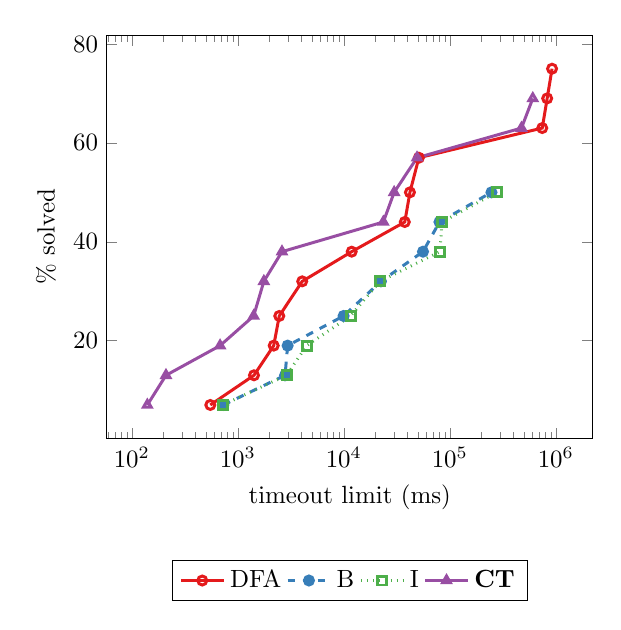
\begin{tikzpicture}[scale=0.9]
      \begin{axis}[
    xmode=log,
    every axis plot/.style={thin},
    xlabel={timeout limit (ms)},
    ylabel={\% solved},
    legend style={at={(0.5,-0.30)},
      anchor=north,legend columns=-1},
    % legend pos=south east,
    cycle list/Set1-6,
            % define fill color for the marker
            mark list fill={.!75!white},
            mark options={solid,scale=0.9},
            cycle multiindex* list={
                Set1-6
                    \nextlist
                [3 of]linestyles
                    \nextlist
                very thick
                \nextlist
                mark=o,
                mark=*,
                mark=square,
                mark=triangle,
                mark=+
            },
    ]

    \addplot
    coordinates {
      (550, 7)
      (1420, 13)
      (2180, 19)
      (2460, 25)
      (4050, 32)
      (11860, 38)
      (37590, 44)
      (42030, 50)
      (51040, 57)
      (744510, 63)
      (828510, 69)
      (921350, 75)
      
    };
    \addplot
    coordinates {
      (730, 7)
      (2790, 13)
      (2950, 19)
      (9950, 25)
      (22390, 32)
      (55820, 38)
      (79890, 44)
      (247070, 50)
      
    };
    \addplot
    coordinates {
      (720, 7)
      (2880, 13)
      (4460, 19)
      (11570, 25)
      (21880, 32)
      (80590, 38)
      (84470, 44)
      (276470, 50)
      
    };
    \addplot
    coordinates {
      (140, 7)
      (210, 13)
      (680, 19)
      (1410, 25)
      (1760, 32)
      (2610, 38)
      (23590, 44)
      (29830, 50)
      (49050, 57)
      (474090, 63)
      (606460, 69)
      
    };
    

    \legend{ DFA, B, I, \textbf{CT} }
  \end{axis}

    \end{tikzpicture}
    \vspace{\baselineskip}
  \end{minipage}\qquad
  \begin{minipage}[b][10cm][s]{0.45\textwidth}
    \centering
    \vfill
    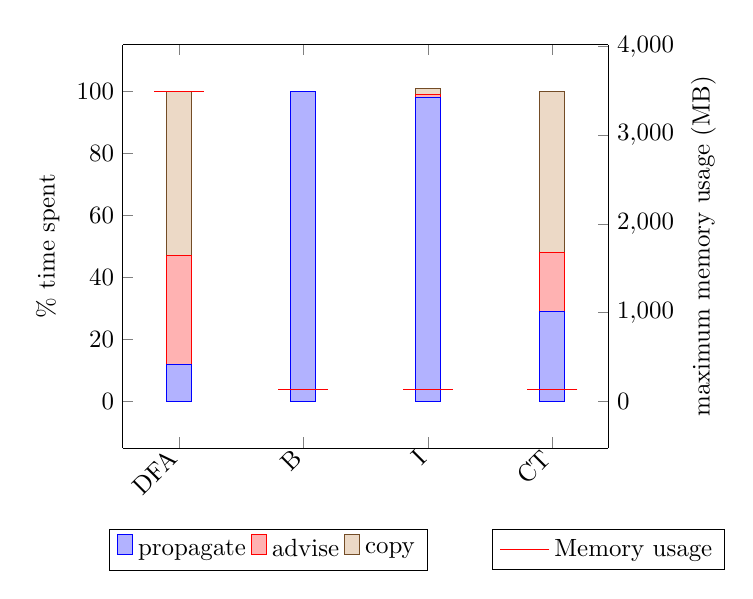
\begin{tikzpicture}[scale=0.9]
  \begin{axis}[
    ybar stacked,
    axis y line*=left,
    ymin=0,
    ymax=100,
    enlargelimits=0.15,
    legend style={at={(0.3,-0.20)},
      anchor=north,legend columns=-1},
    ylabel={\% time spent},
    symbolic x coords={DFA,B,I,CT},
    xtick=data,
    x tick label style={rotate=45,anchor=east},
    ]

    \addplot+[ybar]
      plot coordinates {
        (DFA, 12)
          (B, 100)
          (I, 98)
          (CT, 29)
          
          }; \label{ propagate }
    \addplot+[ybar]
      plot coordinates {
        (DFA, 35)
          (B, 0)
          (I, 1)
          (CT, 19)
          
          }; \label{ advise }
    \addplot+[ybar]
      plot coordinates {
        (DFA, 53)
          (B, 0)
          (I, 2)
          (CT, 52)
          
          }; \label{ copy }
    
      \legend{  }
      
      \addlegendimage{/pgfplots/refstyle=propagate}\addlegendentry{ propagate }
        
        
        \addlegendimage{/pgfplots/refstyle=advise}\addlegendentry{ advise }
        
        
        \addlegendimage{/pgfplots/refstyle=copy}\addlegendentry{ copy }
        
        
        

   \end{axis}

   \begin{axis}[
      axis y line*=right,
      axis x line=none,
      ymin=0,
      enlargelimits=0.15,
      ylabel=maximum memory usage (MB),
      legend style={at={(1.0,-0.20)},
        anchor=north,legend columns=-1},
      symbolic x coords={DFA,B,I,CT}
    ]
    \addplot+[only marks,mark size=10pt,mark=-,,mark options={.!75!red},red]
    plot coordinates {
      (DFA, 3496.42578125)
      (B, 131.5234375)
      (I, 131.4453125)
      (CT, 131.318359375)
      
    };
    \addlegendentry{Memory usage}
  \end{axis}

\end{tikzpicture}

%    \vspace{\baselineskip}
  \end{minipage}\qquad
  \caption{\textbf{ Pigeons Plus }}
\end{figure}
\begin{figure}[t]
  \begin{minipage}[b][10cm][s]{0.45\textwidth}
    \centering
    \vfill
    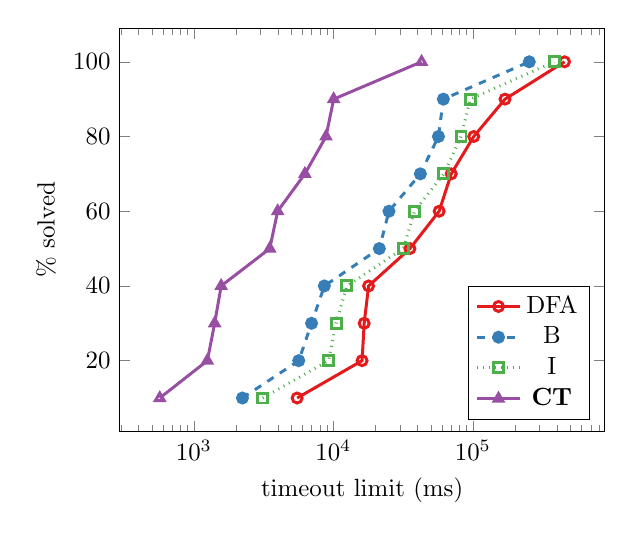
\begin{tikzpicture}[scale=0.9]
      \begin{axis}[
    xmode=log,
    every axis plot/.style={thin},
    xlabel={timeout limit (ms)},
    ylabel={\% solved},
    legend pos=south east,
    cycle list/Set1-6,
            % define fill color for the marker
            mark list fill={.!75!white},
            mark options={solid},
            cycle multiindex* list={
                Set1-6
                    \nextlist
                [3 of]linestyles
                    \nextlist
                very thick
                \nextlist
                mark=o,
                mark=*,
                mark=square,
                mark=triangle,
                mark=+
            },
    ]

    \addplot
    coordinates {
      (5500, 10)
      (16070, 20)
      (16630, 30)
      (17890, 40)
      (35390, 50)
      (57330, 60)
      (69990, 70)
      (101460, 80)
      (169980, 90)
      (453800, 100)
      
    };
    \addplot
    coordinates {
      (2230, 10)
      (5650, 20)
      (6980, 30)
      (8620, 40)
      (21360, 50)
      (25040, 60)
      (42030, 70)
      (56640, 80)
      (61450, 90)
      (253650, 100)
      
    };
    \addplot
    coordinates {
      (3120, 10)
      (9240, 20)
      (10460, 30)
      (12500, 40)
      (31710, 50)
      (38200, 60)
      (61930, 70)
      (82230, 80)
      (95830, 90)
      (382920, 100)
      
    };
    \addplot
    coordinates {
      (570, 10)
      (1250, 20)
      (1410, 30)
      (1570, 40)
      (3500, 50)
      (3990, 60)
      (6250, 70)
      (8860, 80)
      (10050, 90)
      (42870, 100)
      
    };
    

    \legend{ DFA, B, I, \textbf{CT} }
  \end{axis}

    \end{tikzpicture}
    \vspace{\baselineskip}
  \end{minipage}\qquad
  \begin{minipage}[b][10cm][s]{0.45\textwidth}
    \centering
    \vfill
    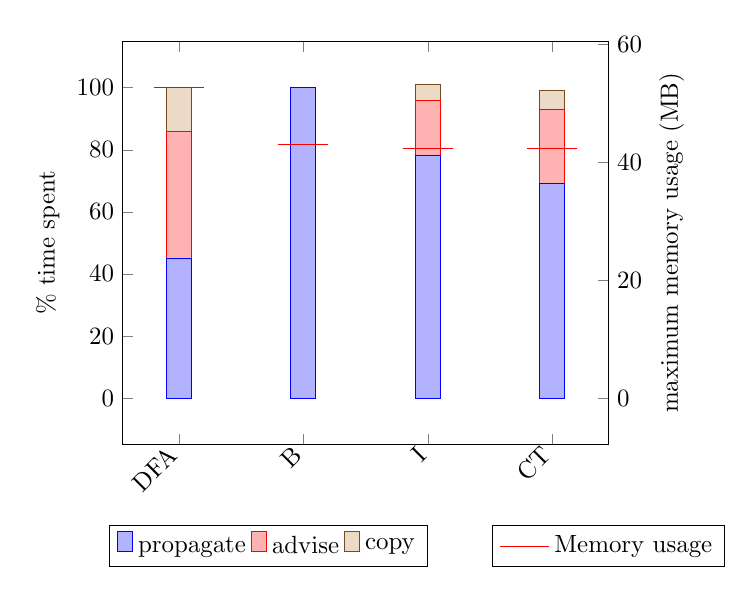
\begin{tikzpicture}[scale=0.9]
  \begin{axis}[
    ybar stacked,
    axis y line*=left,
    ymin=0,
    ymax=100,
    enlargelimits=0.15,
    legend style={at={(0.3,-0.20)},
      anchor=north,legend columns=-1},
    ylabel={\% time spent},
    symbolic x coords={DFA,B,I,CT},
    xtick=data,
    x tick label style={rotate=45,anchor=east},
    ]

    \addplot+[ybar]
      plot coordinates {
        (DFA, 45)
          (B, 100)
          (I, 78)
          (CT, 69)
          
          }; \label{ propagate }
    \addplot+[ybar]
      plot coordinates {
        (DFA, 41)
          (B, 0)
          (I, 18)
          (CT, 24)
          
          }; \label{ advise }
    \addplot+[ybar]
      plot coordinates {
        (DFA, 14)
          (B, 0)
          (I, 5)
          (CT, 6)
          
          }; \label{ copy }
    
      \legend{  }
      
      \addlegendimage{/pgfplots/refstyle=propagate}\addlegendentry{ propagate }
        
        
        \addlegendimage{/pgfplots/refstyle=advise}\addlegendentry{ advise }
        
        
        \addlegendimage{/pgfplots/refstyle=copy}\addlegendentry{ copy }
        
        
        

   \end{axis}

   \begin{axis}[
      axis y line*=right,
      axis x line=none,
      ymin=0,
      enlargelimits=0.15,
      ylabel=maximum memory usage (MB),
      legend style={at={(1.0,-0.20)},
        anchor=north,legend columns=-1},
      symbolic x coords={DFA,B,I,CT}
    ]
    \addplot+[only marks,mark size=10pt,mark=-,,mark options={.!75!red},red]
    plot coordinates {
      (DFA, 52.59765625)
      (B, 42.98828125)
      (I, 42.32421875)
      (CT, 42.32421875)
      
    };
    \addlegendentry{Memory usage}
  \end{axis}

\end{tikzpicture}

%    \vspace{\baselineskip}
  \end{minipage}\qquad
  \caption{\textbf{ Rands JC2500 }}
\end{figure}
\begin{figure}[t]
  \begin{minipage}[b][10cm][s]{0.45\textwidth}
    \centering
    \vfill
    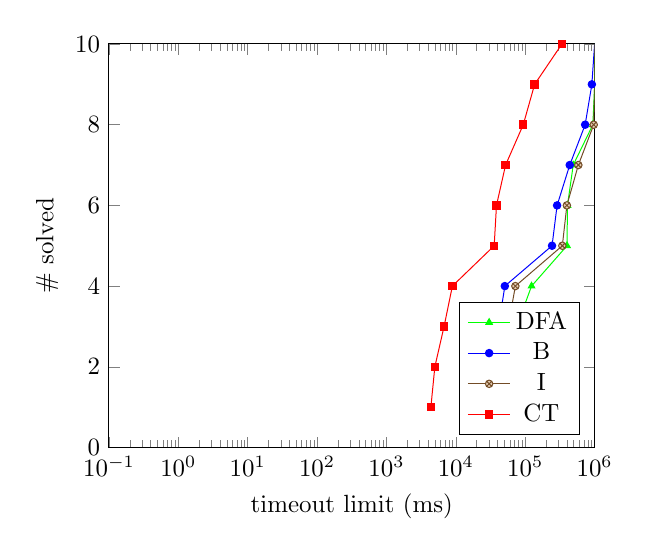
\begin{tikzpicture}[scale=0.9]
      \begin{axis}[
    xmode=log,
    ymin=0,ymax=10,
    xmin=0.1, xmax=1000000,
    every axis plot/.style={thin},
    xlabel={timeout limit (ms)},
    ylabel={\# solved},
    legend pos=south east
    % table/create on use/cumulative distribution/.style={
    %   create col/expr={\pgfmathaccuma + \thisrow{f(x)}}   
    % }
    ]
    \addplot 
    [mark=triangle*,
    mark size=1.5,
    mark options={solid},
    green] 
    coordinates {
    (37271.407, 1)
(63329.760, 2)
(75340.967, 3)
(123361.614, 4)
(400331.140, 5)
(406374.082, 6)
(491965.258, 7)
(943701.318, 8)
(1003127.715, 9)
(1003191.173, 10)
    };

    \addplot 
    [blue,
    mark=*,
    mark size=1.5,
    mark options={solid}]
    coordinates {
    (23487.263, 1)
(31493.067, 2)
(41324.456, 3)
(50843.172, 4)
(243499.863, 5)
(288078.384, 6)
(438078.025, 7)
(731291.713, 8)
(912991.209, 9)
(1000435.280, 10)
    };

    \addplot [brown!60!black,
    mark options={fill=brown!40},
    mark=otimes*,
    mark size=1.5]
    coordinates {
    (31721.470, 1)
(45760.945, 2)
(56699.417, 3)
(72142.510, 4)
(342690.713, 5)
(398501.909, 6)
(583027.925, 7)
(971126.357, 8)
(1000434.235, 9)
(1000435.846, 10)
    };

    \addplot 
    [red,
    mark size=1.5,
    mark=square*]
    coordinates {
    (4367.654, 1)
(4983.151, 2)
(6770.036, 3)
(8914.062, 4)
(35712.233, 5)
(38524.930, 6)
(52111.274, 7)
(93677.132, 8)
(136706.431, 9)
(338099.921, 10)
    };
    \legend{DFA,B,I,CT}
  \end{axis}

    \end{tikzpicture}
    \vspace{\baselineskip}
  \end{minipage}\qquad
  \begin{minipage}[b][10cm][s]{0.45\textwidth}
    \centering
    \vfill
    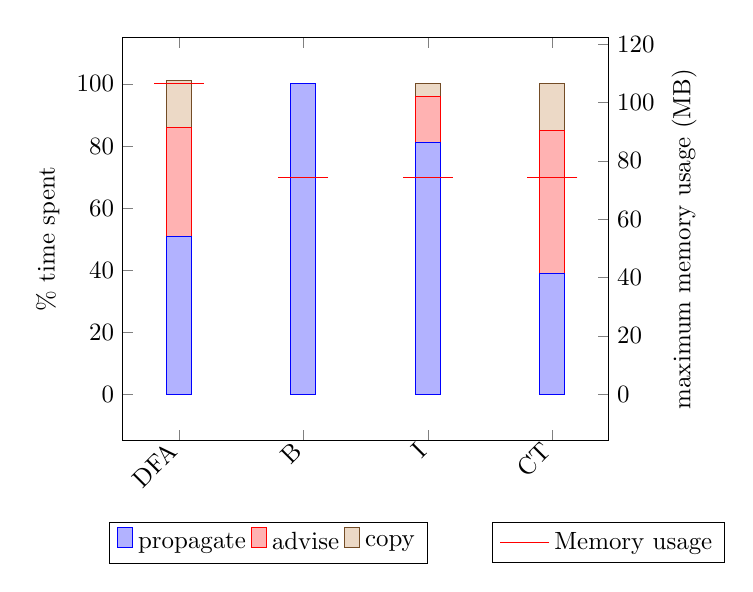
\begin{tikzpicture}[scale=0.9]
  \begin{axis}[
    ybar stacked,
    axis y line*=left,
    ymin=0,
    ymax=100,
    enlargelimits=0.15,
    legend style={at={(0.3,-0.20)},
      anchor=north,legend columns=-1},
    ylabel={\% time spent},
    symbolic x coords={DFA,B,I,CT},
    xtick=data,
    x tick label style={rotate=45,anchor=east},
    ]

    \addplot+[ybar]
      plot coordinates {
        (DFA, 51)
          (B, 100)
          (I, 81)
          (CT, 39)
          
          }; \label{ propagate }
    \addplot+[ybar]
      plot coordinates {
        (DFA, 35)
          (B, 0)
          (I, 15)
          (CT, 46)
          
          }; \label{ advise }
    \addplot+[ybar]
      plot coordinates {
        (DFA, 15)
          (B, 0)
          (I, 4)
          (CT, 15)
          
          }; \label{ copy }
    
      \legend{  }
      
      \addlegendimage{/pgfplots/refstyle=propagate}\addlegendentry{ propagate }
        
        
        \addlegendimage{/pgfplots/refstyle=advise}\addlegendentry{ advise }
        
        
        \addlegendimage{/pgfplots/refstyle=copy}\addlegendentry{ copy }
        
        
        

   \end{axis}

   \begin{axis}[
      axis y line*=right,
      axis x line=none,
      ymin=0,
      enlargelimits=0.15,
      ylabel=maximum memory usage (MB),
      legend style={at={(1.0,-0.20)},
        anchor=north,legend columns=-1},
      symbolic x coords={DFA,B,I,CT}
    ]
    \addplot+[only marks,mark size=10pt,mark=-,,mark options={.!75!red},red]
    plot coordinates {
      (DFA, 106.318359375)
      (B, 74.208984375)
      (I, 74.1796875)
      (CT, 74.111328125)
      
    };
    \addlegendentry{Memory usage}
  \end{axis}

\end{tikzpicture}

%    \vspace{\baselineskip}
  \end{minipage}\qquad
  \caption{\textbf{ Rands JC5000 }}
\end{figure}
\begin{figure}[t]
  \begin{minipage}[b][10cm][s]{0.45\textwidth}
    \centering
    \vfill
    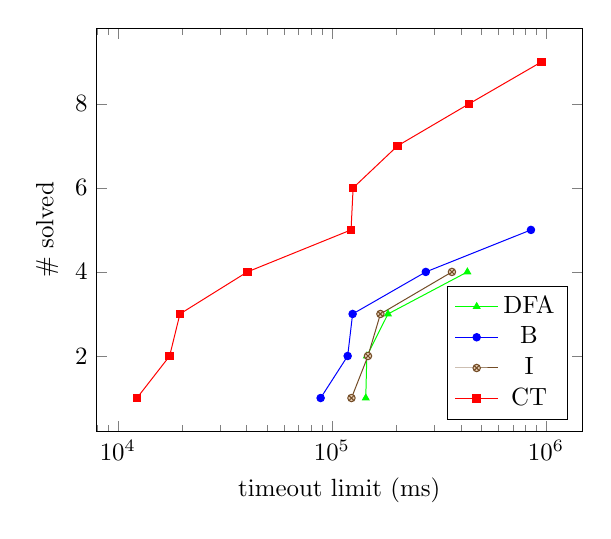
\begin{tikzpicture}[scale=0.9]
      \begin{axis}[
    xmode=log,
    every axis plot/.style={thin},
    xlabel={timeout limit (ms)},
    ylabel={\# solved},
    legend pos=south east
    % table/create on use/cumulative distribution/.style={
    %   create col/expr={\pgfmathaccuma + \thisrow{f(x)}}   
    % }
    ]
    \addplot 
    [mark=triangle*,
    mark size=1.5,
    mark options={solid},
    green] 
    coordinates {
    (143986.214, 1)
(145624.128, 2)
(182844.931, 3)
(429527.079, 4)
% (1004920.333, 5)
% (1005091.406, 6)
% (1005121.020, 7)
% (1005141.458, 8)
% (1005180.694, 9)
% (1005181.896, 10)
    };

    \addplot 
    [blue,
    mark=*,
    mark size=1.5,
    mark options={solid}]
    coordinates {
    (88610.730, 1)
(118513.380, 2)
(124991.902, 3)
(274645.919, 4)
(851285.302, 5)
% (1000662.235, 6)
% (1000665.157, 7)
% (1000667.124, 8)
% (1000679.084, 9)
% (1000680.879, 10)
    };

    \addplot [brown!60!black,
    mark options={fill=brown!40},
    mark=otimes*,
    mark size=1.5]
    coordinates {
    (123456.088, 1)
(147458.027, 2)
(168559.303, 3)
(363926.326, 4)
% (1000644.518, 5)
% (1000648.628, 6)
% (1000660.653, 7)
% (1000663.644, 8)
% (1000669.943, 9)
% (1000672.172, 10)
    };

    \addplot 
    [red,
    mark size=1.5,
    mark=square*]
    coordinates {
    (12283.482, 1)
(17462.103, 2)
(19503.895, 3)
(40266.047, 4)
(122893.209, 5)
(125673.584, 6)
(202682.066, 7)
(437565.193, 8)
(955387.007, 9)
%(1000911.643, 10)
    };
    \legend{DFA,B,I,CT}
  \end{axis}

    \end{tikzpicture}
    \vspace{\baselineskip}
  \end{minipage}\qquad
  \begin{minipage}[b][10cm][s]{0.45\textwidth}
    \centering
    \vfill
    \input{ tba.tex }
%    \vspace{\baselineskip}
  \end{minipage}\qquad
  \caption{\textbf{ Rands JC7500 }}
\end{figure}
\begin{figure}[t]
  \begin{minipage}[b][10cm][s]{0.45\textwidth}
    \centering
    \vfill
    \begin{tikzpicture}[scale=0.9]
      \begin{axis}[
    xmode=log,
    every axis plot/.style={thin},
    xlabel={timeout limit (ms)},
    ylabel={\# solved},
    legend pos=north west
    % table/create on use/cumulative distribution/.style={
    %   create col/expr={\pgfmathaccuma + \thisrow{f(x)}}   
    % }
    ]
    \addplot 
    [mark=triangle*,
    mark size=1.5,
    mark options={solid},
    green] 
    coordinates {
    (339960.449, 1)
(531357.500, 2)
(576758.002, 3)
% (1006830.253, 4)
% (1006953.686, 5)
% (1006987.278, 6)
% (1007012.182, 7)
% (1007040.479, 8)
% (1007166.422, 9)
% (1007385.382, 10)
    };

    \addplot 
    [blue,
    mark=*,
    mark size=1.5,
    mark options={solid}]
    coordinates {
    (227052.199, 1)
(492242.811, 2)
(567372.313, 3)
% (1000877.234, 4)
% (1000889.042, 5)
% (1000892.874, 6)
% (1000895.207, 7)
% (1000911.856, 8)
% (1000913.878, 9)
% (1000928.789, 10)
    };

    \addplot [brown!60!black,
    mark options={fill=brown!40},
    mark=otimes*,
    mark size=1.5]
    coordinates {
    (295287.152, 1)
(650810.991, 2)
(703794.608, 3)
% (1000887.426, 4)
% (1000895.815, 5)
% (1000897.600, 6)
% (1000901.551, 7)
% (1000905.923, 8)
% (1000907.888, 9)
% (1000913.436, 10)
    };

    \addplot 
    [red,
    mark size=1.5,
    mark=square*]
    coordinates {
    (26984.703, 1)
(58304.179, 2)
(65624.179, 3)
(244616.117, 4)
(316746.918, 5)
(490346.243, 6)
(586068.768, 7)
(756641.057, 8)
%(1001171.576, 9)
%(1001192.839, 10)
    };
    \legend{DFA,B,I,CT}
  \end{axis}

    \end{tikzpicture}
    \vspace{\baselineskip}
  \end{minipage}\qquad
  \begin{minipage}[b][10cm][s]{0.45\textwidth}
    \centering
    \vfill
    \begin{tikzpicture}[scale=0.9]
  \begin{axis}[
    ybar stacked,
    axis y line*=left,
    ymin=0,
    ymax=100,
    enlargelimits=0.15,
    legend style={at={(0.3,-0.20)},
      anchor=north,legend columns=-1},
    ylabel={\% time spent},
    symbolic x coords={DFA,B,I,CT},
    xtick=data,
    x tick label style={rotate=45,anchor=east},
    ]

    \addplot+[ybar]
      plot coordinates {
        (DFA, 51)
          (B, 100)
          (I, 88)
          (CT, 41)
          
          }; \label{ propagate }
    \addplot+[ybar]
      plot coordinates {
        (DFA, 33)
          (B, 0)
          (I, 10)
          (CT, 49)
          
          }; \label{ advise }
    \addplot+[ybar]
      plot coordinates {
        (DFA, 16)
          (B, 0)
          (I, 2)
          (CT, 10)
          
          }; \label{ copy }
    
      \legend{  }
      
      \addlegendimage{/pgfplots/refstyle=propagate}\addlegendentry{ propagate }
        
        
        \addlegendimage{/pgfplots/refstyle=advise}\addlegendentry{ advise }
        
        
        \addlegendimage{/pgfplots/refstyle=copy}\addlegendentry{ copy }
        
        
        

   \end{axis}

   \begin{axis}[
      axis y line*=right,
      axis x line=none,
      ymin=0,
      enlargelimits=0.15,
      ylabel=maximum memory usage (MB),
      legend style={at={(1.0,-0.20)},
        anchor=north,legend columns=-1},
      symbolic x coords={DFA,B,I,CT}
    ]
    \addplot+[only marks,mark size=10pt,mark=-,,mark options={.!75!red},red]
    plot coordinates {
      (DFA, 256.767578125)
      (B, 137.119140625)
      (I, 136.5234375)
      (CT, 137.685546875)
      
    };
    \addlegendentry{Memory usage}
  \end{axis}

\end{tikzpicture}

%    \vspace{\baselineskip}
  \end{minipage}\qquad
  \caption{\textbf{ Rands JC10000 }}
\end{figure}
\begin{figure}[t]
  \begin{minipage}[b][10cm][s]{0.45\textwidth}
    \centering
    \vfill
    \begin{tikzpicture}[scale=0.9]
      \begin{axis}[
    xmode=log,
    every axis plot/.style={thin},
    xlabel={timeout limit (ms)},
    ylabel={\# solved},
    legend pos=south east
    % table/create on use/cumulative distribution/.style={
    %   create col/expr={\pgfmathaccuma + \thisrow{f(x)}}   
    % }
    ]
    \addplot 
    [mark=triangle*,
    mark size=1.5,
    mark options={solid},
    green] 
    coordinates {
    (1333.406, 1)
(2072.861, 2)
(2291.811, 3)
(2996.127, 4)
(3390.696, 5)
(4085.322, 6)
(5492.735, 7)
(5494.497, 8)
(5573.341, 9)
(5581.970, 10)
(5861.969, 11)
(5923.068, 12)
(7311.924, 13)
(8965.104, 14)
(9758.067, 15)
    };

    \addplot 
    [blue,
    mark=*,
    mark size=1.5,
    mark options={solid}]
    coordinates {
    (92.898, 1)
(134.489, 2)
(188.799, 3)
(219.819, 4)
(338.413, 5)
(1136.522, 6)
(1172.713, 7)
(2058.962, 8)
(3789.293, 9)
(3824.374, 10)
(3956.922, 11)
(4935.345, 12)
(7773.796, 13)
(11094.603, 14)
(29268.417, 15)
    };

    \addplot [brown!60!black,
    mark options={fill=brown!40},
    mark=otimes*,
    mark size=1.5]
    coordinates {
    (95.886, 1)
(133.264, 2)
(219.206, 3)
(239.481, 4)
(412.639, 5)
(1518.706, 6)
(1684.622, 7)
(2831.549, 8)
(5358.480, 9)
(5425.453, 10)
(5551.804, 11)
(7829.008, 12)
(11095.700, 13)
(16823.395, 14)
(44072.919, 15)
    };

    \addplot 
    [red,
    mark size=1.5,
    mark=square*]
    coordinates {
    (118.884, 1)
(163.180, 2)
(195.126, 3)
(223.383, 4)
(307.055, 5)
(693.402, 6)
(707.378, 7)
(1197.949, 8)
(1889.844, 9)
(1908.499, 10)
(2016.541, 11)
(2302.896, 12)
(3841.743, 13)
(5082.583, 14)
(13144.847, 15)
    };
    \legend{DFA,B,I,CT}
  \end{axis}

    \end{tikzpicture}
    \vspace{\baselineskip}
  \end{minipage}\qquad
  \begin{minipage}[b][10cm][s]{0.45\textwidth}
    \centering
    \vfill
    \begin{tikzpicture}[scale=0.9]
  \begin{axis}[
    ybar stacked,
    axis y line*=left,
    ymin=0,
    ymax=100,
    enlargelimits=0.15,
    legend style={at={(0.3,-0.20)},
      anchor=north,legend columns=-1},
    ylabel={\% time spent},
    symbolic x coords={DFA,B,I,CT},
    xtick=data,
    x tick label style={rotate=45,anchor=east},
    ]

    \addplot+[ybar]
      plot coordinates {
        (DFA, 41)
          (B, 90)
          (I, 35)
          (CT, 41)
          
          }; \label{ propagate }
    \addplot+[ybar]
      plot coordinates {
        (DFA, 38)
          (B, 0)
          (I, 27)
          (CT, 42)
          
          }; \label{ advise }
    \addplot+[ybar]
      plot coordinates {
        (DFA, 21)
          (B, 10)
          (I, 38)
          (CT, 17)
          
          }; \label{ copy }
    
      \legend{  }
      
      \addlegendimage{/pgfplots/refstyle=propagate}\addlegendentry{ propagate }
        
        
        \addlegendimage{/pgfplots/refstyle=advise}\addlegendentry{ advise }
        
        
        \addlegendimage{/pgfplots/refstyle=copy}\addlegendentry{ copy }
        
        
        

   \end{axis}

   \begin{axis}[
      axis y line*=right,
      axis x line=none,
      ymin=0,
      enlargelimits=0.15,
      ylabel=maximum memory usage (MB),
      legend style={at={(1.0,-0.20)},
        anchor=north,legend columns=-1},
      symbolic x coords={DFA,B,I,CT}
    ]
    \addplot+[only marks,mark size=10pt,mark=-,,mark options={.!75!red},red]
    plot coordinates {
      (DFA, 75.87890625)
      (B, 53.798828125)
      (I, 53.740234375)
      (CT, 55.185546875)
      
    };
    \addlegendentry{Memory usage}
  \end{axis}

\end{tikzpicture}

%    \vspace{\baselineskip}
  \end{minipage}\qquad
  \caption{\textbf{ TSP 20 }}
\end{figure}
\begin{figure}[t]
  \begin{minipage}[b][10cm][s]{0.45\textwidth}
    \centering
    \vfill
    \begin{tikzpicture}[scale=0.9]
      \begin{axis}[
    xmode=log,
    every axis plot/.style={thin},
    xlabel={timeout limit (ms)},
    ylabel={\% solved},
    legend pos=south east,
    cycle list/Set1-6,
            % define fill color for the marker
            mark list fill={.!75!white},
            mark options={solid},
            cycle multiindex* list={
                Set1-6
                    \nextlist
                [3 of]linestyles
                    \nextlist
                very thick
                \nextlist
                mark=o,
                mark=*,
                mark=square,
                mark=triangle,
                mark=+
            },
    ]

    \addplot
    coordinates {
      (2310, 7)
      (3050, 14)
      (3280, 20)
      (3480, 27)
      (4110, 34)
      (4640, 40)
      (6230, 47)
      (6550, 54)
      (6570, 60)
      (7330, 67)
      (7780, 74)
      (8210, 80)
      (8270, 87)
      (8360, 94)
      (12510, 100)
      
    };
    \addplot
    coordinates {
      (610, 7)
      (820, 14)
      (990, 20)
      (1200, 27)
      (1250, 34)
      (1530, 40)
      (8430, 47)
      (8550, 54)
      (13190, 60)
      (14750, 67)
      (22720, 74)
      (26230, 80)
      (34060, 87)
      (99550, 94)
      (196100, 100)
      
    };
    \addplot
    coordinates {
      (720, 7)
      (1040, 14)
      (1180, 20)
      (1570, 27)
      (1610, 34)
      (2060, 40)
      (11310, 47)
      (12140, 54)
      (17130, 60)
      (19510, 67)
      (31680, 74)
      (37680, 80)
      (47500, 87)
      (136970, 94)
      (261960, 100)
      
    };
    \addplot
    coordinates {
      (400, 7)
      (550, 14)
      (560, 20)
      (630, 27)
      (690, 34)
      (800, 40)
      (3710, 47)
      (3760, 54)
      (5650, 60)
      (5810, 67)
      (9780, 74)
      (10930, 80)
      (13290, 87)
      (43980, 94)
      (77540, 100)
      
    };
    

    \legend{ DFA, B, I, \textbf{CT} }
  \end{axis}

    \end{tikzpicture}
    \vspace{\baselineskip}
  \end{minipage}\qquad
  \begin{minipage}[b][10cm][s]{0.45\textwidth}
    \centering
    \vfill
    \begin{tikzpicture}[scale=0.9]
  \begin{axis}[
    ybar stacked,
    axis y line*=left,
    ymin=0,
    ymax=100,
    enlargelimits=0.15,
    legend style={at={(0.3,-0.20)},
      anchor=north,legend columns=-1},
    ylabel={\% time spent},
    symbolic x coords={DFA,B,I,CT},
    xtick=data,
    x tick label style={rotate=45,anchor=east},
    ]

    \addplot+[ybar]
      plot coordinates {
        (DFA, 25)
          (B, 73)
          (I, 38)
          (CT, 58)
          
          }; \label{ propagate }
    \addplot+[ybar]
      plot coordinates {
        (DFA, 45)
          (B, 0)
          (I, 19)
          (CT, 33)
          
          }; \label{ advise }
    \addplot+[ybar]
      plot coordinates {
        (DFA, 30)
          (B, 27)
          (I, 43)
          (CT, 8)
          
          }; \label{ copy }
    
      \legend{  }
      
      \addlegendimage{/pgfplots/refstyle=propagate}\addlegendentry{ propagate }
        
        
        \addlegendimage{/pgfplots/refstyle=advise}\addlegendentry{ advise }
        
        
        \addlegendimage{/pgfplots/refstyle=copy}\addlegendentry{ copy }
        
        
        

   \end{axis}

   \begin{axis}[
      axis y line*=right,
      axis x line=none,
      ymin=0,
      enlargelimits=0.15,
      ylabel=maximum memory usage (MB),
      legend style={at={(1.0,-0.20)},
        anchor=north,legend columns=-1},
      symbolic x coords={DFA,B,I,CT}
    ]
    \addplot+[only marks,mark size=10pt,mark=-,,mark options={.!75!red},red]
    plot coordinates {
      (DFA, 98.22265625)
      (B, 74.228515625)
      (I, 74.2578125)
      (CT, 75.83984375)
      
    };
    \addlegendentry{Memory usage}
  \end{axis}

\end{tikzpicture}

%    \vspace{\baselineskip}
  \end{minipage}\qquad
  \caption{\textbf{ TSP 25 }}
\end{figure}
\begin{figure}[t]
  \begin{minipage}[b][10cm][s]{0.45\textwidth}
    \centering
    \vfill
    \begin{tikzpicture}[scale=0.9]
      \begin{axis}[
    xmode=log,
    every axis plot/.style={thin},
    xlabel={timeout limit (ms)},
    ylabel={\# solved},
    legend pos=south east
    % table/create on use/cumulative distribution/.style={
    %   create col/expr={\pgfmathaccuma + \thisrow{f(x)}}   
    % }
    ]
    \addplot 
    [mark=triangle*,
    mark size=1.5,
    mark options={solid},
    green] 
    coordinates {
    (8323.942, 1)
(9080.418, 2)
(9457.327, 3)
(9611.154, 4)
(11157.909, 5)
(12122.318, 6)
(12269.578, 7)
(12569.631, 8)
(12613.425, 9)
(13987.860, 10)
(15538.867, 11)
    };

    \addplot 
    [blue,
    mark=*,
    mark size=1.5,
    mark options={solid}]
    coordinates {
    (1188.206, 1)
(1289.021, 2)
(1636.318, 3)
(1725.962, 4)
(2339.887, 5)
(6481.991, 6)
(7504.933, 7)
(22155.924, 8)
(23009.793, 9)
(40756.444, 10)
(181399.438, 11)
    };

    \addplot [brown!60!black,
    mark options={fill=brown!40},
    mark=otimes*,
    mark size=1.5]
    coordinates {
    (1175.718, 1)
(1354.438, 2)
(2353.159, 3)
(2454.453, 4)
(3594.396, 5)
(12379.752, 6)
(16444.353, 7)
(47478.184, 8)
(49773.525, 9)
(89852.322, 10)
(425399.368, 11)
    };

    \addplot 
    [red,
    mark size=1.5,
    mark=square*]
    coordinates {
    (1794.640, 1)
(1795.355, 2)
(1951.150, 3)
(1965.074, 4)
(2212.001, 5)
(2673.018, 6)
(2822.171, 7)
(6633.134, 8)
(7933.220, 9)
(13389.469, 10)
(45079.672, 11)
    };
    \legend{DFA,B,I,CT}
  \end{axis}

    \end{tikzpicture}
    \vspace{\baselineskip}
  \end{minipage}\qquad
  \begin{minipage}[b][10cm][s]{0.45\textwidth}
    \centering
    \vfill
    \begin{tikzpicture}[scale=0.9]
  \begin{axis}[
    ybar stacked,
    axis y line*=left,
    ymin=0,
    ymax=100,
    enlargelimits=0.15,
    legend style={at={(0.3,-0.20)},
      anchor=north,legend columns=-1},
    ylabel={\% time spent},
    symbolic x coords={DFA,B,I,CT},
    xtick=data,
    x tick label style={rotate=45,anchor=east},
    ]

    \addplot+[ybar]
      plot coordinates {
        (DFA, 32)
          (B, 50)
          (I, 16)
          (CT, 62)
          
          }; \label{ propagate }
    \addplot+[ybar]
      plot coordinates {
        (DFA, 45)
          (B, 0)
          (I, 10)
          (CT, 30)
          
          }; \label{ advise }
    \addplot+[ybar]
      plot coordinates {
        (DFA, 23)
          (B, 50)
          (I, 74)
          (CT, 6)
          
          }; \label{ copy }
    
      \legend{  }
      
      \addlegendimage{/pgfplots/refstyle=propagate}\addlegendentry{ propagate }
        
        
        \addlegendimage{/pgfplots/refstyle=advise}\addlegendentry{ advise }
        
        
        \addlegendimage{/pgfplots/refstyle=copy}\addlegendentry{ copy }
        
        
        

   \end{axis}

   \begin{axis}[
      axis y line*=right,
      axis x line=none,
      ymin=0,
      enlargelimits=0.15,
      ylabel=maximum memory usage (MB),
      legend style={at={(1.0,-0.20)},
        anchor=north,legend columns=-1},
      symbolic x coords={DFA,B,I,CT}
    ]
    \addplot+[only marks,mark size=10pt,mark=-,,mark options={.!75!red},red]
    plot coordinates {
      (DFA, 295.546875)
      (B, 269.814453125)
      (I, 291.89453125)
      (CT, 269.619140625)
      
    };
    \addlegendentry{Memory usage}
  \end{axis}

\end{tikzpicture}

%    \vspace{\baselineskip}
  \end{minipage}\qquad
  \caption{\textbf{ TSP Quat 20 }}
\end{figure}





% \section{Profiling}

% \begin{tikzpicture}[scale=0.9]
  
  \begin{axis}[
    ybar stacked,
    every axis plot/.append style={fill},
    axis y line*=left,
    ymin=0,
    enlargelimits=0.15,
    ylabel=maximum memory usage (MB),
    legend style={at={(0.1,-0.40)},
      anchor=north,legend columns=-1},
    symbolic x coords={DFA,B,I,CT},
    cycle list name=RdYlGn-9
    ]
    \addplot+[ybar,bar width=10pt,mark=none,xshift=-10pt]
    plot coordinates {
      (DFA, 13.73046875)
      (B, 13.369140625)
      (I, 13.45703125)
      (CT, 13.154296875)
      
    };
    \addlegendentry{Memory usage}
  \end{axis}

  \begin{axis}[
    ybar stacked,
    every axis plot/.append style={fill},
    axis x line=none,
    axis y line*=right,
    ymin=0,
    ymax=100,
    enlargelimits=0.15,
    legend style={at={(0.8,-0.40)},
      anchor=north,legend columns=-1},
    ylabel={\% time spent},
    symbolic x coords={DFA,B,I,CT},
    xtick=data,
    cycle list name=Reds-4,
    x tick label style={rotate=45,anchor=east},
    ]

    \addplot+[ybar,xshift=10pt]
      plot coordinates {
        (DFA, 6)
          (B, 41)
          (I, 9)
          (CT, 16)
          
          }; \label{ propagate }
    \addplot+[ybar,xshift=10pt]
      plot coordinates {
        (DFA, 19)
          (B, 0)
          (I, 9)
          (CT, 8)
          
          }; \label{ advise }
    \addplot+[ybar,xshift=10pt]
      plot coordinates {
        (DFA, 75)
          (B, 59)
          (I, 82)
          (CT, 76)
          
          }; \label{ copy }
    
      \legend{  }
      
      \addlegendimage{/pgfplots/refstyle=propagate}\addlegendentry{ propagate }
        
        \addlegendimage{/pgfplots/refstyle=advise}\addlegendentry{ advise }
        
        \addlegendimage{/pgfplots/refstyle=copy}\addlegendentry{ copy }
        
        

   \end{axis}

\end{tikzpicture}

% \begin{tikzpicture}[scale=0.9]
  
  \begin{axis}[
    ybar stacked,
    every axis plot/.append style={fill},
    axis y line*=left,
    ymin=0,
    enlargelimits=0.15,
    ylabel=maximum memory usage (MB),
    legend style={at={(0.1,-0.40)},
      anchor=north,legend columns=-1},
    symbolic x coords={DFA,B,I,CT},
    cycle list name=RdYlGn-9
    ]
    \addplot+[ybar,bar width=10pt,mark=none,xshift=-10pt]
    plot coordinates {
      (DFA, 8.115234375)
      (B, 7.373046875)
      (I, 8.5546875)
      (CT, 7.685546875)
      
    };
    \addlegendentry{Memory usage}
  \end{axis}

  \begin{axis}[
    ybar stacked,
    every axis plot/.append style={fill},
    axis x line=none,
    axis y line*=right,
    ymin=0,
    ymax=100,
    enlargelimits=0.15,
    legend style={at={(0.8,-0.40)},
      anchor=north,legend columns=-1},
    ylabel={\% time spent},
    symbolic x coords={DFA,B,I,CT},
    xtick=data,
    cycle list name=Reds-4,
    x tick label style={rotate=45,anchor=east},
    ]

    \addplot+[ybar,xshift=10pt]
      plot coordinates {
        (DFA, 4)
          (B, 28)
          (I, 6)
          (CT, 6)
          
          }; \label{ propagate }
    \addplot+[ybar,xshift=10pt]
      plot coordinates {
        (DFA, 13)
          (B, 0)
          (I, 8)
          (CT, 5)
          
          }; \label{ advise }
    \addplot+[ybar,xshift=10pt]
      plot coordinates {
        (DFA, 83)
          (B, 72)
          (I, 86)
          (CT, 89)
          
          }; \label{ copy }
    
      \legend{  }
      
      \addlegendimage{/pgfplots/refstyle=propagate}\addlegendentry{ propagate }
        
        \addlegendimage{/pgfplots/refstyle=advise}\addlegendentry{ advise }
        
        \addlegendimage{/pgfplots/refstyle=copy}\addlegendentry{ copy }
        
        

   \end{axis}

\end{tikzpicture}

% \begin{tikzpicture}[scale=0.9]
  
  \begin{axis}[
    ybar stacked,
    every axis plot/.append style={fill},
    axis y line*=left,
    ymin=0,
    enlargelimits=0.15,
    ylabel=maximum memory usage (MB),
    legend style={at={(0.1,-0.40)},
      anchor=north,legend columns=-1},
    symbolic x coords={DFA,B,I,CT},
    cycle list name=RdYlGn-9
    ]
    \addplot+[ybar,bar width=10pt,mark=none,xshift=-10pt]
    plot coordinates {
      (DFA, 38.75)
      (B, 36.1328125)
      (I, 35.9375)
      (CT, 35.8984375)
      
    };
    \addlegendentry{Memory usage}
  \end{axis}

  \begin{axis}[
    ybar stacked,
    every axis plot/.append style={fill},
    axis x line=none,
    axis y line*=right,
    ymin=0,
    ymax=100,
    enlargelimits=0.15,
    legend style={at={(0.8,-0.40)},
      anchor=north,legend columns=-1},
    ylabel={\% time spent},
    symbolic x coords={DFA,B,I,CT},
    xtick=data,
    cycle list name=Reds-4,
    x tick label style={rotate=45,anchor=east},
    ]

    \addplot+[ybar,xshift=10pt]
      plot coordinates {
        (DFA, 25)
          (B, 94)
          (I, 62)
          (CT, 50)
          
          }; \label{ propagate }
    \addplot+[ybar,xshift=10pt]
      plot coordinates {
        (DFA, 25)
          (B, 0)
          (I, 12)
          (CT, 17)
          
          }; \label{ advise }
    \addplot+[ybar,xshift=10pt]
      plot coordinates {
        (DFA, 51)
          (B, 6)
          (I, 26)
          (CT, 34)
          
          }; \label{ copy }
    
      \legend{  }
      
      \addlegendimage{/pgfplots/refstyle=propagate}\addlegendentry{ propagate }
        
        \addlegendimage{/pgfplots/refstyle=advise}\addlegendentry{ advise }
        
        \addlegendimage{/pgfplots/refstyle=copy}\addlegendentry{ copy }
        
        

   \end{axis}

\end{tikzpicture}

% \begin{tikzpicture}[scale=0.9]
  \begin{axis}[
    ybar stacked,
    axis y line*=left,
    ymin=0,
    ymax=100,
    enlargelimits=0.15,
    legend style={at={(0.3,-0.20)},
      anchor=north,legend columns=-1},
    ylabel={\% time spent},
    symbolic x coords={DFA,B,I,CT},
    xtick=data,
    x tick label style={rotate=45,anchor=east},
    ]

    \addplot+[ybar]
      plot coordinates {
        (DFA, 21)
          (B, 80)
          (I, 31)
          (CT, 32)
          
          }; \label{ propagate }
    \addplot+[ybar]
      plot coordinates {
        (DFA, 34)
          (B, 0)
          (I, 22)
          (CT, 16)
          
          }; \label{ advise }
    \addplot+[ybar]
      plot coordinates {
        (DFA, 45)
          (B, 20)
          (I, 47)
          (CT, 52)
          
          }; \label{ copy }
    
      \legend{  }
      
      \addlegendimage{/pgfplots/refstyle=propagate}\addlegendentry{ propagate }
        
        
        \addlegendimage{/pgfplots/refstyle=advise}\addlegendentry{ advise }
        
        
        \addlegendimage{/pgfplots/refstyle=copy}\addlegendentry{ copy }
        
        
        

   \end{axis}

   \begin{axis}[
      axis y line*=right,
      axis x line=none,
      ymin=0,
      enlargelimits=0.15,
      ylabel=maximum memory usage (MB),
      legend style={at={(1.0,-0.20)},
        anchor=north,legend columns=-1},
      symbolic x coords={DFA,B,I,CT}
    ]
    \addplot+[only marks,mark size=10pt,mark=-,,mark options={.!75!red},red]
    plot coordinates {
      (DFA, 13.53515625)
      (B, 13.310546875)
      (I, 13.2421875)
      (CT, 13.115234375)
      
    };
    \addlegendentry{Memory usage}
  \end{axis}

\end{tikzpicture}

% \begin{tikzpicture}[scale=0.9]
  
  \begin{axis}[
    ybar stacked,
    every axis plot/.append style={fill},
    axis y line*=left,
    ymin=0,
    enlargelimits=0.15,
    ylabel=maximum memory usage (MB),
    legend style={at={(0.1,-0.40)},
      anchor=north,legend columns=-1},
    symbolic x coords={DFA,B,I,CT},
    cycle list name=RdYlGn-9
    ]
    \addplot+[ybar,bar width=10pt,mark=none,xshift=-10pt]
    plot coordinates {
      (DFA, 40.15625)
      (B, 28.49609375)
      (I, 28.310546875)
      (CT, 28.30078125)
      
    };
    \addlegendentry{Memory usage}
  \end{axis}

  \begin{axis}[
    ybar stacked,
    every axis plot/.append style={fill},
    axis x line=none,
    axis y line*=right,
    ymin=0,
    ymax=100,
    enlargelimits=0.15,
    legend style={at={(0.8,-0.40)},
      anchor=north,legend columns=-1},
    ylabel={\% time spent},
    symbolic x coords={DFA,B,I,CT},
    xtick=data,
    cycle list name=Reds-4,
    x tick label style={rotate=45,anchor=east},
    ]

    \addplot+[ybar,xshift=10pt]
      plot coordinates {
        (DFA, 73)
          (B, 98)
          (I, 81)
          (CT, 68)
          
          }; \label{ propagate }
    \addplot+[ybar,xshift=10pt]
      plot coordinates {
        (DFA, 17)
          (B, 0)
          (I, 15)
          (CT, 24)
          
          }; \label{ advise }
    \addplot+[ybar,xshift=10pt]
      plot coordinates {
        (DFA, 10)
          (B, 2)
          (I, 4)
          (CT, 8)
          
          }; \label{ copy }
    
      \legend{  }
      
      \addlegendimage{/pgfplots/refstyle=propagate}\addlegendentry{ propagate }
        
        \addlegendimage{/pgfplots/refstyle=advise}\addlegendentry{ advise }
        
        \addlegendimage{/pgfplots/refstyle=copy}\addlegendentry{ copy }
        
        

   \end{axis}

\end{tikzpicture}

% \begin{tikzpicture}[scale=0.9]
  \begin{axis}[
    ybar stacked,
    axis y line*=left,
    ymin=0,
    ymax=100,
    enlargelimits=0.15,
    legend style={at={(0.3,-0.20)},
      anchor=north,legend columns=-1},
    ylabel={\% time spent},
    symbolic x coords={DFA,B,I,CT},
    xtick=data,
    x tick label style={rotate=45,anchor=east},
    ]

    \addplot+[ybar]
      plot coordinates {
        (DFA, 56)
          (B, 99)
          (I, 90)
          (CT, 50)
          
          }; \label{ propagate }
    \addplot+[ybar]
      plot coordinates {
        (DFA, 22)
          (B, 0)
          (I, 8)
          (CT, 20)
          
          }; \label{ advise }
    \addplot+[ybar]
      plot coordinates {
        (DFA, 22)
          (B, 1)
          (I, 2)
          (CT, 31)
          
          }; \label{ copy }
    
      \legend{  }
      
      \addlegendimage{/pgfplots/refstyle=propagate}\addlegendentry{ propagate }
        
        
        \addlegendimage{/pgfplots/refstyle=advise}\addlegendentry{ advise }
        
        
        \addlegendimage{/pgfplots/refstyle=copy}\addlegendentry{ copy }
        
        
        

   \end{axis}

   \begin{axis}[
      axis y line*=right,
      axis x line=none,
      ymin=0,
      enlargelimits=0.15,
      ylabel=maximum memory usage (MB),
      legend style={at={(1.0,-0.20)},
        anchor=north,legend columns=-1},
      symbolic x coords={DFA,B,I,CT}
    ]
    \addplot+[only marks,mark size=10pt,mark=-,,mark options={.!75!red},red]
    plot coordinates {
      (DFA, 61.30859375)
      (B, 30.0390625)
      (I, 30.0390625)
      (CT, 30.29296875)
      
    };
    \addlegendentry{Memory usage}
  \end{axis}

\end{tikzpicture}

% \begin{tikzpicture}[scale=0.9]
  \begin{axis}[
    ybar stacked,
    axis y line*=left,
    ymin=0,
    ymax=100,
    enlargelimits=0.15,
    legend style={at={(0.3,-0.20)},
      anchor=north,legend columns=-1},
    ylabel={\% time spent},
    symbolic x coords={DFA,B,I,CT},
    xtick=data,
    x tick label style={rotate=45,anchor=east},
    ]

    \addplot+[ybar]
      plot coordinates {
        (DFA, 26)
          (B, 94)
          (I, 35)
          (CT, 37)
          
          }; \label{ propagate }
    \addplot+[ybar]
      plot coordinates {
        (DFA, 54)
          (B, 0)
          (I, 45)
          (CT, 40)
          
          }; \label{ advise }
    \addplot+[ybar]
      plot coordinates {
        (DFA, 19)
          (B, 6)
          (I, 20)
          (CT, 24)
          
          }; \label{ copy }
    
      \legend{  }
      
      \addlegendimage{/pgfplots/refstyle=propagate}\addlegendentry{ propagate }
        
        
        \addlegendimage{/pgfplots/refstyle=advise}\addlegendentry{ advise }
        
        
        \addlegendimage{/pgfplots/refstyle=copy}\addlegendentry{ copy }
        
        
        

   \end{axis}

   \begin{axis}[
      axis y line*=right,
      axis x line=none,
      ymin=0,
      enlargelimits=0.15,
      ylabel=maximum memory usage (MB),
      legend style={at={(1.0,-0.20)},
        anchor=north,legend columns=-1},
      symbolic x coords={DFA,B,I,CT}
    ]
    \addplot+[only marks,mark size=10pt,mark=-,,mark options={.!75!red},red]
    plot coordinates {
      (DFA, 5660.048828125)
      (B, 76.962890625)
      (I, 76.62109375)
      (CT, 76.416015625)
      
    };
    \addlegendentry{Memory usage}
  \end{axis}

\end{tikzpicture}

% \begin{tikzpicture}[scale=0.9]
  \begin{axis}[
    ybar stacked,
    axis y line*=left,
    ymin=0,
    ymax=100,
    enlargelimits=0.15,
    legend style={at={(0.3,-0.20)},
      anchor=north,legend columns=-1},
    ylabel={\% time spent},
    symbolic x coords={DFA,B,I,CT},
    xtick=data,
    x tick label style={rotate=45,anchor=east},
    ]

    \addplot+[ybar]
      plot coordinates {
        (DFA, 32)
          (B, 50)
          (I, 16)
          (CT, 62)
          
          }; \label{ propagate }
    \addplot+[ybar]
      plot coordinates {
        (DFA, 45)
          (B, 0)
          (I, 10)
          (CT, 30)
          
          }; \label{ advise }
    \addplot+[ybar]
      plot coordinates {
        (DFA, 23)
          (B, 50)
          (I, 74)
          (CT, 6)
          
          }; \label{ copy }
    
      \legend{  }
      
      \addlegendimage{/pgfplots/refstyle=propagate}\addlegendentry{ propagate }
        
        
        \addlegendimage{/pgfplots/refstyle=advise}\addlegendentry{ advise }
        
        
        \addlegendimage{/pgfplots/refstyle=copy}\addlegendentry{ copy }
        
        
        

   \end{axis}

   \begin{axis}[
      axis y line*=right,
      axis x line=none,
      ymin=0,
      enlargelimits=0.15,
      ylabel=maximum memory usage (MB),
      legend style={at={(1.0,-0.20)},
        anchor=north,legend columns=-1},
      symbolic x coords={DFA,B,I,CT}
    ]
    \addplot+[only marks,mark size=10pt,mark=-,,mark options={.!75!red},red]
    plot coordinates {
      (DFA, 295.546875)
      (B, 269.814453125)
      (I, 291.89453125)
      (CT, 269.619140625)
      
    };
    \addlegendentry{Memory usage}
  \end{axis}

\end{tikzpicture}

% \begin{tikzpicture}[scale=0.9]
  \begin{axis}[
    ybar stacked,
    axis y line*=left,
    ymin=0,
    ymax=100,
    enlargelimits=0.15,
    legend style={at={(0.3,-0.20)},
      anchor=north,legend columns=-1},
    ylabel={\% time spent},
    symbolic x coords={DFA,B,I,CT},
    xtick=data,
    x tick label style={rotate=45,anchor=east},
    ]

    \addplot+[ybar]
      plot coordinates {
        (DFA, 41)
          (B, 90)
          (I, 35)
          (CT, 41)
          
          }; \label{ propagate }
    \addplot+[ybar]
      plot coordinates {
        (DFA, 38)
          (B, 0)
          (I, 27)
          (CT, 42)
          
          }; \label{ advise }
    \addplot+[ybar]
      plot coordinates {
        (DFA, 21)
          (B, 10)
          (I, 38)
          (CT, 17)
          
          }; \label{ copy }
    
      \legend{  }
      
      \addlegendimage{/pgfplots/refstyle=propagate}\addlegendentry{ propagate }
        
        
        \addlegendimage{/pgfplots/refstyle=advise}\addlegendentry{ advise }
        
        
        \addlegendimage{/pgfplots/refstyle=copy}\addlegendentry{ copy }
        
        
        

   \end{axis}

   \begin{axis}[
      axis y line*=right,
      axis x line=none,
      ymin=0,
      enlargelimits=0.15,
      ylabel=maximum memory usage (MB),
      legend style={at={(1.0,-0.20)},
        anchor=north,legend columns=-1},
      symbolic x coords={DFA,B,I,CT}
    ]
    \addplot+[only marks,mark size=10pt,mark=-,,mark options={.!75!red},red]
    plot coordinates {
      (DFA, 75.87890625)
      (B, 53.798828125)
      (I, 53.740234375)
      (CT, 55.185546875)
      
    };
    \addlegendentry{Memory usage}
  \end{axis}

\end{tikzpicture}

% \begin{tikzpicture}[scale=0.9]
  \begin{axis}[
    ybar stacked,
    axis y line*=left,
    ymin=0,
    ymax=100,
    enlargelimits=0.15,
    legend style={at={(0.3,-0.20)},
      anchor=north,legend columns=-1},
    ylabel={\% time spent},
    symbolic x coords={DFA,B,I,CT},
    xtick=data,
    x tick label style={rotate=45,anchor=east},
    ]

    \addplot+[ybar]
      plot coordinates {
        (DFA, 25)
          (B, 73)
          (I, 38)
          (CT, 58)
          
          }; \label{ propagate }
    \addplot+[ybar]
      plot coordinates {
        (DFA, 45)
          (B, 0)
          (I, 19)
          (CT, 33)
          
          }; \label{ advise }
    \addplot+[ybar]
      plot coordinates {
        (DFA, 30)
          (B, 27)
          (I, 43)
          (CT, 8)
          
          }; \label{ copy }
    
      \legend{  }
      
      \addlegendimage{/pgfplots/refstyle=propagate}\addlegendentry{ propagate }
        
        
        \addlegendimage{/pgfplots/refstyle=advise}\addlegendentry{ advise }
        
        
        \addlegendimage{/pgfplots/refstyle=copy}\addlegendentry{ copy }
        
        
        

   \end{axis}

   \begin{axis}[
      axis y line*=right,
      axis x line=none,
      ymin=0,
      enlargelimits=0.15,
      ylabel=maximum memory usage (MB),
      legend style={at={(1.0,-0.20)},
        anchor=north,legend columns=-1},
      symbolic x coords={DFA,B,I,CT}
    ]
    \addplot+[only marks,mark size=10pt,mark=-,,mark options={.!75!red},red]
    plot coordinates {
      (DFA, 98.22265625)
      (B, 74.228515625)
      (I, 74.2578125)
      (CT, 75.83984375)
      
    };
    \addlegendentry{Memory usage}
  \end{axis}

\end{tikzpicture}

% \begin{tikzpicture}[scale=0.9]
  \begin{axis}[
    ybar stacked,
    axis y line*=left,
    ymin=0,
    ymax=100,
    enlargelimits=0.15,
    legend style={at={(0.3,-0.20)},
      anchor=north,legend columns=-1},
    ylabel={\% time spent},
    symbolic x coords={DFA,B,I,CT},
    xtick=data,
    x tick label style={rotate=45,anchor=east},
    ]

    \addplot+[ybar]
      plot coordinates {
        (DFA, 33)
          (B, 93)
          (I, 24)
          (CT, 45)
          
          }; \label{ propagate }
    \addplot+[ybar]
      plot coordinates {
        (DFA, 43)
          (B, 0)
          (I, 48)
          (CT, 43)
          
          }; \label{ advise }
    \addplot+[ybar]
      plot coordinates {
        (DFA, 24)
          (B, 7)
          (I, 28)
          (CT, 12)
          
          }; \label{ copy }
    
      \legend{  }
      
      \addlegendimage{/pgfplots/refstyle=propagate}\addlegendentry{ propagate }
        
        
        \addlegendimage{/pgfplots/refstyle=advise}\addlegendentry{ advise }
        
        
        \addlegendimage{/pgfplots/refstyle=copy}\addlegendentry{ copy }
        
        
        

   \end{axis}

   \begin{axis}[
      axis y line*=right,
      axis x line=none,
      ymin=0,
      enlargelimits=0.15,
      ylabel=maximum memory usage (MB),
      legend style={at={(1.0,-0.20)},
        anchor=north,legend columns=-1},
      symbolic x coords={DFA,B,I,CT}
    ]
    \addplot+[only marks,mark size=10pt,mark=-,,mark options={.!75!red},red]
    plot coordinates {
      (DFA, 23.61328125)
      (B, 23.193359375)
      (I, 28.92578125)
      (CT, 24.921875)
      
    };
    \addlegendentry{Memory usage}
  \end{axis}

\end{tikzpicture}

% \begin{tikzpicture}[scale=0.9]
  
  \begin{axis}[
    ybar stacked,
    every axis plot/.append style={fill},
    axis y line*=left,
    ymin=0,
    enlargelimits=0.15,
    ylabel=maximum memory usage (MB),
    legend style={at={(0.1,-0.40)},
      anchor=north,legend columns=-1},
    symbolic x coords={DFA,B,I,CT},
    cycle list name=RdYlGn-9
    ]
    \addplot+[ybar,bar width=10pt,mark=none,xshift=-10pt]
    plot coordinates {
      (DFA, 126.279296875)
      (B, 125.76171875)
      (I, 125.634765625)
      (CT, 125.458984375)
      
    };
    \addlegendentry{Memory usage}
  \end{axis}

  \begin{axis}[
    ybar stacked,
    every axis plot/.append style={fill},
    axis x line=none,
    axis y line*=right,
    ymin=0,
    ymax=100,
    enlargelimits=0.15,
    legend style={at={(0.8,-0.40)},
      anchor=north,legend columns=-1},
    ylabel={\% time spent},
    symbolic x coords={DFA,B,I,CT},
    xtick=data,
    cycle list name=Reds-4,
    x tick label style={rotate=45,anchor=east},
    ]

    \addplot+[ybar,xshift=10pt]
      plot coordinates {
        (DFA, 30)
          (B, 80)
          (I, 12)
          (CT, 47)
          
          }; \label{ propagate }
    \addplot+[ybar,xshift=10pt]
      plot coordinates {
        (DFA, 38)
          (B, 0)
          (I, 31)
          (CT, 33)
          
          }; \label{ advise }
    \addplot+[ybar,xshift=10pt]
      plot coordinates {
        (DFA, 32)
          (B, 20)
          (I, 57)
          (CT, 20)
          
          }; \label{ copy }
    
      \legend{  }
      
      \addlegendimage{/pgfplots/refstyle=propagate}\addlegendentry{ propagate }
        
        \addlegendimage{/pgfplots/refstyle=advise}\addlegendentry{ advise }
        
        \addlegendimage{/pgfplots/refstyle=copy}\addlegendentry{ copy }
        
        

   \end{axis}

\end{tikzpicture}

% \begin{tikzpicture}[scale=0.9]
  
  \begin{axis}[
    ybar stacked,
    every axis plot/.append style={fill},
    axis y line*=left,
    ymin=0,
    enlargelimits=0.15,
    ylabel=maximum memory usage (MB),
    legend style={at={(0.1,-0.40)},
      anchor=north,legend columns=-1},
    symbolic x coords={DFA,B,I,CT},
    cycle list name=RdYlGn-9
    ]
    \addplot+[ybar,bar width=10pt,mark=none,xshift=-10pt]
    plot coordinates {
      (DFA, 262.36328125)
      (B, 262.265625)
      (I, 262.158203125)
      (CT, 262.03125)
      
    };
    \addlegendentry{Memory usage}
  \end{axis}

  \begin{axis}[
    ybar stacked,
    every axis plot/.append style={fill},
    axis x line=none,
    axis y line*=right,
    ymin=0,
    ymax=100,
    enlargelimits=0.15,
    legend style={at={(0.8,-0.40)},
      anchor=north,legend columns=-1},
    ylabel={\% time spent},
    symbolic x coords={DFA,B,I,CT},
    xtick=data,
    cycle list name=Reds-4,
    x tick label style={rotate=45,anchor=east},
    ]

    \addplot+[ybar,xshift=10pt]
      plot coordinates {
        (DFA, 32)
          (B, 88)
          (I, 23)
          (CT, 42)
          
          }; \label{ propagate }
    \addplot+[ybar,xshift=10pt]
      plot coordinates {
        (DFA, 39)
          (B, 0)
          (I, 31)
          (CT, 53)
          
          }; \label{ advise }
    \addplot+[ybar,xshift=10pt]
      plot coordinates {
        (DFA, 29)
          (B, 12)
          (I, 46)
          (CT, 5)
          
          }; \label{ copy }
    
      \legend{  }
      
      \addlegendimage{/pgfplots/refstyle=propagate}\addlegendentry{ propagate }
        
        \addlegendimage{/pgfplots/refstyle=advise}\addlegendentry{ advise }
        
        \addlegendimage{/pgfplots/refstyle=copy}\addlegendentry{ copy }
        
        

   \end{axis}

\end{tikzpicture}

% \begin{tikzpicture}[scale=0.9]
  \begin{axis}[
    ybar stacked,
    ymin=0,
    ymax=100,
    enlargelimits=0.15,
    legend style={at={(0.5,-0.20)},
      anchor=north,legend columns=-1},
    ylabel={\% time spent},
    symbolic x coords={DFA,B,I,CT},
    xtick=data,
    x tick label style={rotate=45,anchor=east},
    ]

    \addplot+[ybar]
      plot coordinates {
        (DFA, 32)
          (B, 100)
          (I, 95)
          (CT, 47)
          
          };
    \addplot+[ybar]
      plot coordinates {
        (DFA, 41)
          (B, 0)
          (I, 4)
          (CT, 35)
          
          };
    \addplot+[ybar]
      plot coordinates {
        (DFA, 27)
          (B, 0)
          (I, 1)
          (CT, 17)
          
          };
    

     \legend{Propagate,Advise,Copy}

          \end{axis}

\end{tikzpicture}

% \begin{tikzpicture}[scale=0.9]
  
  \begin{axis}[
    ybar stacked,
    every axis plot/.append style={fill},
    axis y line*=left,
    ymin=0,
    enlargelimits=0.15,
    ylabel=maximum memory usage (MB),
    legend style={at={(0.1,-0.40)},
      anchor=north,legend columns=-1},
    symbolic x coords={DFA,B,I,CT},
    cycle list name=RdYlGn-9
    ]
    \addplot+[ybar,bar width=10pt,mark=none,xshift=-10pt]
    plot coordinates {
      (DFA, 4864.921875)
      (B, 705.224609375)
      (I, 703.9453125)
      (CT, 704.62890625)
      
    };
    \addlegendentry{Memory usage}
  \end{axis}

  \begin{axis}[
    ybar stacked,
    every axis plot/.append style={fill},
    axis x line=none,
    axis y line*=right,
    ymin=0,
    ymax=100,
    enlargelimits=0.15,
    legend style={at={(0.8,-0.40)},
      anchor=north,legend columns=-1},
    ylabel={\% time spent},
    symbolic x coords={DFA,B,I,CT},
    xtick=data,
    cycle list name=Reds-4,
    x tick label style={rotate=45,anchor=east},
    ]

    \addplot+[ybar,xshift=10pt]
      plot coordinates {
        (DFA, 43)
          (B, 100)
          (I, 96)
          (CT, 33)
          
          }; \label{ propagate }
    \addplot+[ybar,xshift=10pt]
      plot coordinates {
        (DFA, 34)
          (B, 0)
          (I, 3)
          (CT, 50)
          
          }; \label{ advise }
    \addplot+[ybar,xshift=10pt]
      plot coordinates {
        (DFA, 23)
          (B, 0)
          (I, 1)
          (CT, 17)
          
          }; \label{ copy }
    
      \legend{  }
      
      \addlegendimage{/pgfplots/refstyle=propagate}\addlegendentry{ propagate }
        
        \addlegendimage{/pgfplots/refstyle=advise}\addlegendentry{ advise }
        
        \addlegendimage{/pgfplots/refstyle=copy}\addlegendentry{ copy }
        
        

   \end{axis}

\end{tikzpicture}

% \begin{tikzpicture}[scale=0.9]
  \begin{axis}[
    ybar stacked,
    axis y line*=left,
    ymin=0,
    ymax=100,
    enlargelimits=0.15,
    legend style={at={(0.3,-0.20)},
      anchor=north,legend columns=-1},
    ylabel={\% time spent},
    symbolic x coords={DFA,B,I,CT},
    xtick=data,
    x tick label style={rotate=45,anchor=east},
    ]

    \addplot+[ybar]
      plot coordinates {
        (DFA, 12)
          (B, 100)
          (I, 98)
          (CT, 29)
          
          }; \label{ propagate }
    \addplot+[ybar]
      plot coordinates {
        (DFA, 35)
          (B, 0)
          (I, 1)
          (CT, 19)
          
          }; \label{ advise }
    \addplot+[ybar]
      plot coordinates {
        (DFA, 53)
          (B, 0)
          (I, 2)
          (CT, 52)
          
          }; \label{ copy }
    
      \legend{  }
      
      \addlegendimage{/pgfplots/refstyle=propagate}\addlegendentry{ propagate }
        
        
        \addlegendimage{/pgfplots/refstyle=advise}\addlegendentry{ advise }
        
        
        \addlegendimage{/pgfplots/refstyle=copy}\addlegendentry{ copy }
        
        
        

   \end{axis}

   \begin{axis}[
      axis y line*=right,
      axis x line=none,
      ymin=0,
      enlargelimits=0.15,
      ylabel=maximum memory usage (MB),
      legend style={at={(1.0,-0.20)},
        anchor=north,legend columns=-1},
      symbolic x coords={DFA,B,I,CT}
    ]
    \addplot+[only marks,mark size=10pt,mark=-,,mark options={.!75!red},red]
    plot coordinates {
      (DFA, 3496.42578125)
      (B, 131.5234375)
      (I, 131.4453125)
      (CT, 131.318359375)
      
    };
    \addlegendentry{Memory usage}
  \end{axis}

\end{tikzpicture}

% \begin{tikzpicture}[scale=0.9]
  \begin{axis}[
    ybar stacked,
    axis y line*=left,
    ymin=0,
    ymax=100,
    enlargelimits=0.15,
    legend style={at={(0.3,-0.20)},
      anchor=north,legend columns=-1},
    ylabel={\% time spent},
    symbolic x coords={DFA,B,I,CT},
    xtick=data,
    x tick label style={rotate=45,anchor=east},
    ]

    \addplot+[ybar]
      plot coordinates {
        (DFA, 47)
          (B, 100)
          (I, 92)
          (CT, 21)
          
          }; \label{ propagate }
    \addplot+[ybar]
      plot coordinates {
        (DFA, 38)
          (B, 0)
          (I, 7)
          (CT, 77)
          
          }; \label{ advise }
    \addplot+[ybar]
      plot coordinates {
        (DFA, 15)
          (B, 0)
          (I, 1)
          (CT, 3)
          
          }; \label{ copy }
    
      \legend{  }
      
      \addlegendimage{/pgfplots/refstyle=propagate}\addlegendentry{ propagate }
        
        
        \addlegendimage{/pgfplots/refstyle=advise}\addlegendentry{ advise }
        
        
        \addlegendimage{/pgfplots/refstyle=copy}\addlegendentry{ copy }
        
        
        

   \end{axis}

   \begin{axis}[
      axis y line*=right,
      axis x line=none,
      ymin=0,
      enlargelimits=0.15,
      ylabel=maximum memory usage (MB),
      legend style={at={(1.0,-0.20)},
        anchor=north,legend columns=-1},
      symbolic x coords={DFA,B,I,CT}
    ]
    \addplot+[only marks,mark size=10pt,mark=-,,mark options={.!75!red},red]
    plot coordinates {
      (DFA, 1842.919921875)
      (B, 704.638671875)
      (I, 703.1640625)
      (CT, 703.515625)
      
    };
    \addlegendentry{Memory usage}
  \end{axis}

\end{tikzpicture}

% \begin{tikzpicture}[scale=0.9]
  \begin{axis}[
    ybar stacked,
    axis y line*=left,
    ymin=0,
    ymax=100,
    enlargelimits=0.15,
    legend style={at={(0.3,-0.20)},
      anchor=north,legend columns=-1},
    ylabel={\% time spent},
    symbolic x coords={DFA,B,I,CT},
    xtick=data,
    x tick label style={rotate=45,anchor=east},
    ]

    \addplot+[ybar]
      plot coordinates {
        (DFA, 45)
          (B, 100)
          (I, 78)
          (CT, 69)
          
          }; \label{ propagate }
    \addplot+[ybar]
      plot coordinates {
        (DFA, 41)
          (B, 0)
          (I, 18)
          (CT, 24)
          
          }; \label{ advise }
    \addplot+[ybar]
      plot coordinates {
        (DFA, 14)
          (B, 0)
          (I, 5)
          (CT, 6)
          
          }; \label{ copy }
    
      \legend{  }
      
      \addlegendimage{/pgfplots/refstyle=propagate}\addlegendentry{ propagate }
        
        
        \addlegendimage{/pgfplots/refstyle=advise}\addlegendentry{ advise }
        
        
        \addlegendimage{/pgfplots/refstyle=copy}\addlegendentry{ copy }
        
        
        

   \end{axis}

   \begin{axis}[
      axis y line*=right,
      axis x line=none,
      ymin=0,
      enlargelimits=0.15,
      ylabel=maximum memory usage (MB),
      legend style={at={(1.0,-0.20)},
        anchor=north,legend columns=-1},
      symbolic x coords={DFA,B,I,CT}
    ]
    \addplot+[only marks,mark size=10pt,mark=-,,mark options={.!75!red},red]
    plot coordinates {
      (DFA, 52.59765625)
      (B, 42.98828125)
      (I, 42.32421875)
      (CT, 42.32421875)
      
    };
    \addlegendentry{Memory usage}
  \end{axis}

\end{tikzpicture}

% \begin{tikzpicture}[scale=0.9]
  \begin{axis}[
    ybar stacked,
    axis y line*=left,
    ymin=0,
    ymax=100,
    enlargelimits=0.15,
    legend style={at={(0.3,-0.20)},
      anchor=north,legend columns=-1},
    ylabel={\% time spent},
    symbolic x coords={DFA,B,I,CT},
    xtick=data,
    x tick label style={rotate=45,anchor=east},
    ]

    \addplot+[ybar]
      plot coordinates {
        (DFA, 51)
          (B, 100)
          (I, 81)
          (CT, 39)
          
          }; \label{ propagate }
    \addplot+[ybar]
      plot coordinates {
        (DFA, 35)
          (B, 0)
          (I, 15)
          (CT, 46)
          
          }; \label{ advise }
    \addplot+[ybar]
      plot coordinates {
        (DFA, 15)
          (B, 0)
          (I, 4)
          (CT, 15)
          
          }; \label{ copy }
    
      \legend{  }
      
      \addlegendimage{/pgfplots/refstyle=propagate}\addlegendentry{ propagate }
        
        
        \addlegendimage{/pgfplots/refstyle=advise}\addlegendentry{ advise }
        
        
        \addlegendimage{/pgfplots/refstyle=copy}\addlegendentry{ copy }
        
        
        

   \end{axis}

   \begin{axis}[
      axis y line*=right,
      axis x line=none,
      ymin=0,
      enlargelimits=0.15,
      ylabel=maximum memory usage (MB),
      legend style={at={(1.0,-0.20)},
        anchor=north,legend columns=-1},
      symbolic x coords={DFA,B,I,CT}
    ]
    \addplot+[only marks,mark size=10pt,mark=-,,mark options={.!75!red},red]
    plot coordinates {
      (DFA, 106.318359375)
      (B, 74.208984375)
      (I, 74.1796875)
      (CT, 74.111328125)
      
    };
    \addlegendentry{Memory usage}
  \end{axis}

\end{tikzpicture}

% \begin{tikzpicture}[scale=0.9]
  \begin{axis}[
    ybar stacked,
    axis y line*=left,
    ymin=0,
    ymax=100,
    enlargelimits=0.15,
    legend style={at={(0.3,-0.20)},
      anchor=north,legend columns=-1},
    ylabel={\% time spent},
    symbolic x coords={DFA,B,I,CT},
    xtick=data,
    x tick label style={rotate=45,anchor=east},
    ]

    \addplot+[ybar]
      plot coordinates {
        (DFA, 51)
          (B, 100)
          (I, 88)
          (CT, 41)
          
          }; \label{ propagate }
    \addplot+[ybar]
      plot coordinates {
        (DFA, 33)
          (B, 0)
          (I, 10)
          (CT, 49)
          
          }; \label{ advise }
    \addplot+[ybar]
      plot coordinates {
        (DFA, 16)
          (B, 0)
          (I, 2)
          (CT, 10)
          
          }; \label{ copy }
    
      \legend{  }
      
      \addlegendimage{/pgfplots/refstyle=propagate}\addlegendentry{ propagate }
        
        
        \addlegendimage{/pgfplots/refstyle=advise}\addlegendentry{ advise }
        
        
        \addlegendimage{/pgfplots/refstyle=copy}\addlegendentry{ copy }
        
        
        

   \end{axis}

   \begin{axis}[
      axis y line*=right,
      axis x line=none,
      ymin=0,
      enlargelimits=0.15,
      ylabel=maximum memory usage (MB),
      legend style={at={(1.0,-0.20)},
        anchor=north,legend columns=-1},
      symbolic x coords={DFA,B,I,CT}
    ]
    \addplot+[only marks,mark size=10pt,mark=-,,mark options={.!75!red},red]
    plot coordinates {
      (DFA, 256.767578125)
      (B, 137.119140625)
      (I, 136.5234375)
      (CT, 137.685546875)
      
    };
    \addlegendentry{Memory usage}
  \end{axis}

\end{tikzpicture}


\end{document}

%%% Local Variables:
%%% mode: 
%%% TeX-master: t
%%% End:

% OscaR source code:
% https://bitbucket.org/oscarlib/oscar/src/40e25aafba8f9b0ab06029449350a2a9d1614854/oscar-algo/src/main/scala/oscar/algo/reversible/ReversibleSparseBitSet.scala?at=dev&fileviewer=file-view-default
% https://bitbucket.org/oscarlib/oscar/src/40e25aafba8f9b0ab06029449350a2a9d1614854/oscar-cp/src/main/scala/oscar/cp/constraints/tables/TableCT.scala?at=dev&fileviewer=file-view-default3

% course note in constraint programming
% http://user.it.uu.se/~pierref/courses/COCP/slides/CourseNotes.pdf

% M-x reftex-parse-all
% F1 b
% M-x customize-group reftex

% Hash Functions
% https://en.wikipedia.org/wiki/Pairing_function
% https://www.cs.hmc.edu/~geoff/classes/hmc.cs070.200101/homework10/hashfuncs.html
% http://stackoverflow.com/questions/37918951/what-is-a-minimal-hash-function-for-a-pair-of-ints-that-has-low-chance-of-collis

